\documentclass[aspectratio=169,11pt]{beamer}
\makeatletter\def\input@path{{theme/}}\makeatother
\usetheme[progressbar=foot,sectionpage=none,numbering=fraction,block=transparent]{metropolis}
\usepackage[spanish,es-nodecimaldot]{babel}
\usepackage{amsmath,amssymb,booktabs,array,graphicx,tikz,adjustbox}
\usetikzlibrary{arrows.meta,positioning}
\usepackage{iftex}
\ifPDFTeX\usepackage[T1]{fontenc}\usepackage[utf8]{inputenc}\usepackage{lmodern}\else
\setsansfont[Path=fonts/,ItalicFont=FiraSans-LightItalic.otf,BoldFont=FiraSans-Regular.otf,BoldItalicFont=FiraSans-Italic.otf]{FiraSans-Light.otf}
\setmonofont[Path=fonts/,BoldFont=FiraMono-Medium.otf]{FiraMono-Regular.otf}\fi
\definecolor{accent}{HTML}{087E8B}
\definecolor{ink}{HTML}{23313B}
\definecolor{muted}{HTML}{5B6770}
\setbeamercolor{normal text}{fg=ink,bg=white}
\setbeamercolor{alerted text}{fg=accent}
\setbeamercolor{frametitle}{fg=ink,bg=white}
\setbeamercolor{progress bar}{fg=accent,bg=black!10}
\setbeamercolor{title separator}{fg=accent}
\setbeamercolor{structure}{fg=accent}
\setbeamercolor{background canvas}{bg=white}
\setbeamerfont{frametitle}{size=\large}
\setbeamerfont{footnote}{size=\scriptsize}
\setbeamersize{text margin left=8mm,text margin right=8mm}
\setbeamertemplate{navigation symbols}{}
\setbeamertemplate{frame numbering}{\insertframenumber/\insertmainframenumber}
\makeatletter
\setbeamertemplate{progress bar in head/foot}{%
  \nointerlineskip
  \setlength{\metropolis@progressinheadfoot}{\paperwidth * \ratio{\insertframenumber pt}{\insertmainframenumber pt}}%
  \begin{beamercolorbox}[wd=\paperwidth]{progress bar in head/foot}
  \begin{tikzpicture}
  \fill[bg] (0,0) rectangle (\paperwidth,\metropolis@progressinheadfoot@linewidth);
  \fill[fg] (0,0) rectangle (\metropolis@progressinheadfoot,\metropolis@progressinheadfoot@linewidth);
  \end{tikzpicture}\end{beamercolorbox}}
\makeatother
\setbeamertemplate{caption}{\insertcaption}
\setbeamertemplate{note page}[plain]
\setbeameroption{hide notes}
\setlength{\emergencystretch}{1em}
\setlength{\tabcolsep}{3pt}
\newcommand{\figcaption}[1]{{\fontsize{8}{9.5}\selectfont\textcolor{muted}{#1}\par}}
\hypersetup{pdfauthor={Matías Escobar y Martín Herrera},pdftitle={Autómatas y Control Discreto: Proyecto integrador de grúa portuaria},colorlinks=true,urlcolor=accent}
\title{Autómatas y Control Discreto}
\subtitle{Diseño, desarrollo, integración y validación del sistema}
\author{Matías Escobar \quad Martín Herrera}
\institute{Prof: Ing. Gabriel L. Julián}
\date{13 de octubre de 2026}
\titlegraphic{\hfill
\includegraphics[width=3.7cm]{imagenes/r_000.png}}
\newcommand{\figurefooter}[1]{\par\nointerlineskip\vbox to 0pt{\vss\hbox{\begin{tikzpicture}[remember picture,overlay]
\node[anchor=south west,text width=12.8cm,inner sep=0pt,font=\fontsize{7.5}{8.6}\selectfont,text=muted] at ([xshift=8mm,yshift=3.8mm]current page.south west) {#1};
\end{tikzpicture}}}}
\newsavebox{\diagramstore}
\newcommand{\diagramfit}[1]{\begingroup\hyphenpenalty=10000\relax\adjustbox{max totalsize={\linewidth}{3.95cm}}{#1}\endgroup}
\tikzset{sfstate/.style={draw=accent!75,fill=black!4,rounded corners=2pt,align=center,font=\fontsize{10}{11}\selectfont,minimum height=9mm,text width=2.5cm},sfcstep/.style={draw=ink,fill=black!4,align=center,font=\fontsize{10}{11}\selectfont,minimum height=6mm,text width=3.0cm},guard/.style={font=\fontsize{9}{10}\selectfont,text=orange!75!black,align=left},flow/.style={-{Stealth},draw=accent,semithick},wire/.style={draw=ink,semithick}}

\begin{document}
\section{Apertura}
\begin{frame}[plain]
\setlength{\parskip}{0pt}
\vspace*{2mm}
\hfill
\includegraphics[width=3.7cm,height=1.2cm,keepaspectratio]{imagenes/r_000.png}\par
\vspace{3mm}
{\fontsize{19}{22}\selectfont\bfseries Autómatas y Control Discreto\par}
\vspace{3mm}
{\fontsize{14}{17}\selectfont Proyecto integrador: Control de Accionamientos y\\Automatización de Grúa Portuaria de Muelle tipo Pórtico\par}
\vspace{3mm}\textcolor{accent}{\rule{\linewidth}{0.8pt}}\par\vspace{2mm}
{\fontsize{12}{14}\selectfont Diseño, desarrollo, integración y validación del sistema\par}
\vspace{5mm}
Matías Escobar \quad Martín Herrera\par
\vspace{2mm}{\small Prof: Ing. Gabriel L. Julián\par}
\vfill{\small 13 de octubre de 2026\par}
\vspace*{4mm}
\note{Presentar la asignatura, el proyecto integrador, los integrantes y el docente. Indicar que se recorrerá el diseño, desarrollo, integración y validación del sistema.}
\end{frame}
\begin{frame}[t,label=slide2]{Recorrido de la exposición}
\relax
\begin{columns}[T,onlytextwidth]\column{.48\textwidth}\fontsize{9.2}{11.2}\selectfont\textbf{Planta y regulación}\par\begin{enumerate}
\item \textbf{Maniobra y requisitos.} Recorridos, cargas, límites y objetivo productivo.
\item \textbf{Modelo físico.} Cables elásticos, contacto, accionamientos, frenos y sensores.
\item \textbf{Carro.} Reducción mecánica, cascada, polos y corrección anti-sway.
\item \textbf{Izaje.} Deducción en longitud, compensación de tensión y asignación de tres ganancias.
\item \textbf{Pruebas aisladas e integración.} Seguimiento, balanceo y excitación del modo flexible.
\end{enumerate}\column{.48\textwidth}\fontsize{9.2}{11.2}\selectfont\textbf{Coordinación y pruebas}\par\begin{enumerate}
\setcounter{enumi}{5}
\item \textbf{Supervisor.} Modos, toma y entrega, pesaje, barrido y frenos.
\item \textbf{Planificación automática.} Perfil, despeje, referencias suaves y reloj común.
\item \textbf{Implementación.} Seguridad, CODESYS, estimadores y MC de dos ejes.
\item \textbf{Pruebas MIL y SIL.} Maniobra completa y comparación con/sin anti-sway.
\item \textbf{Productividad y alcance.} Ciclo inicial, ajuste y trabajos futuros.
\end{enumerate}\end{columns}
\note{Presentar primero los fenómenos físicos y luego las aproximaciones de diseño. El diagnóstico de la integración explica por qué se acondicionan las referencias. Anunciar cómo se relacionan los bancos: las pruebas aisladas caracterizan la regulación, las completas verifican la secuencia y el ciclo cerrado permite estimar productividad.}
\end{frame}

\begin{frame}[t,label=slide3]{La maniobra que debe resolver el sistema}
\begin{columns}[T,onlytextwidth]
\column{0.49\textwidth}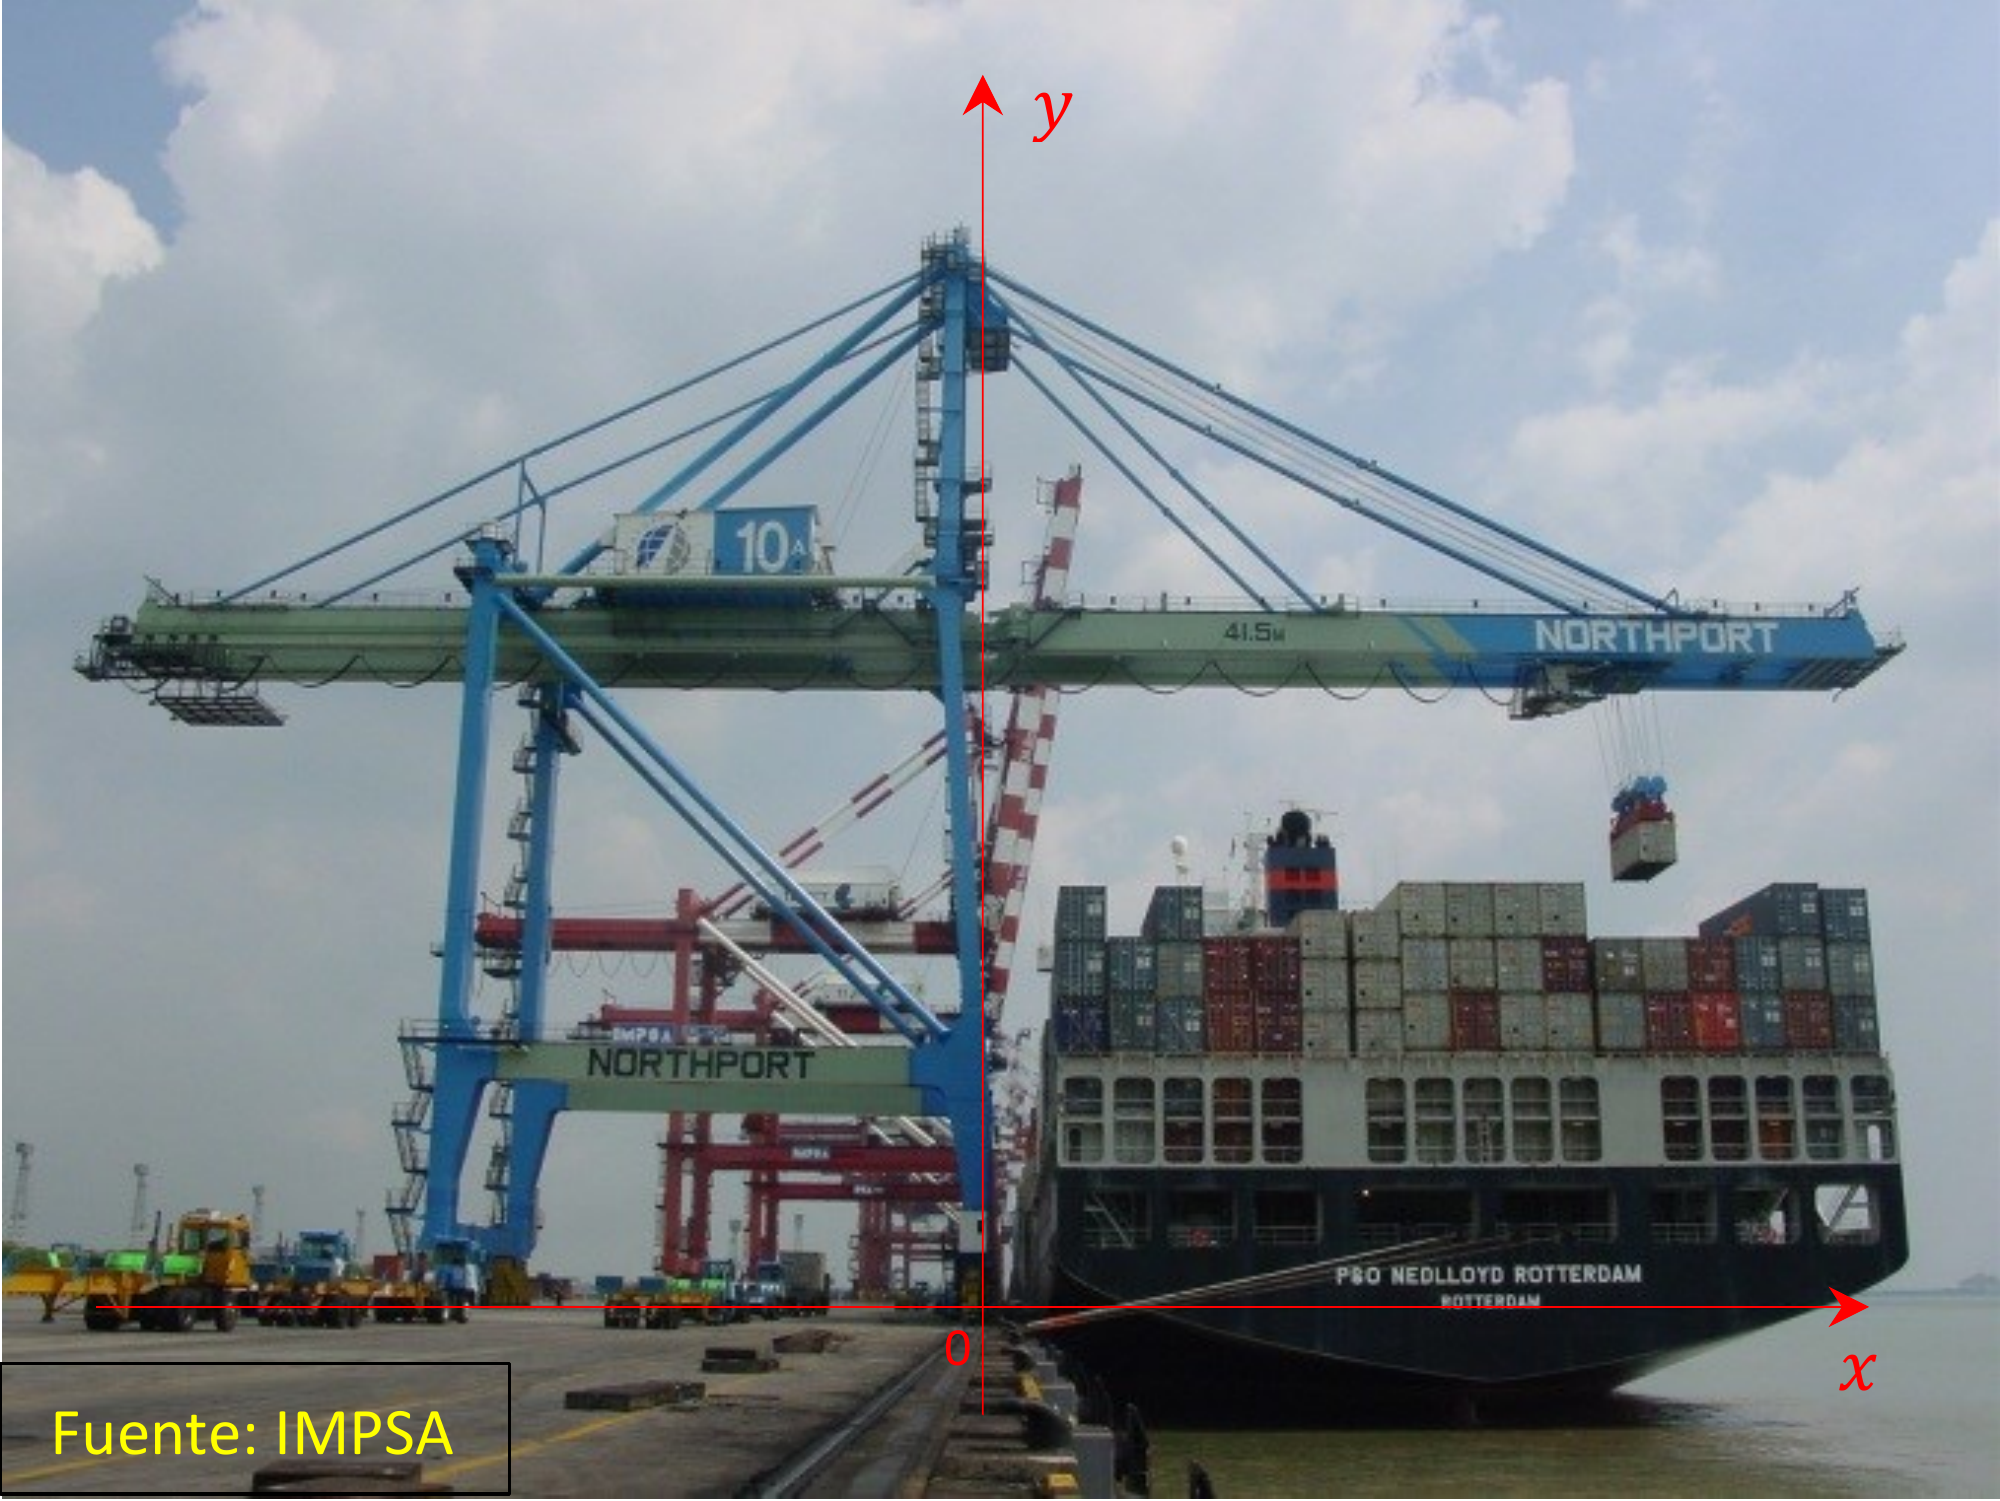
\includegraphics[width=.98\linewidth,height=4.9cm,keepaspectratio,trim=0 180 0 0,clip]{imagenes/r_001.png}
\column{0.47\textwidth}\begin{itemize}
\item Transferencia semiautomática entre muelle y buque.
\item Toma y descenso final bajo supervisión manual.
\item Traslado automático con izaje y carro coordinados.
\item Carga suspendida: balanceo, obstáculos y cambios de masa.
\end{itemize}
\end{columns}
\note{Ubicar físicamente los dos ejes. Explicar por qué seguir una posición no garantiza que la carga quede estable ni que el recorrido sea seguro.}
\end{frame}
\begin{frame}[t,label=slide4]{Requisitos mecánicos y operativos}
\begin{center}
{\small\renewcommand{\arraystretch}{1.0}
\begin{tabular}{lrr}\toprule
Magnitud & Carro & Izaje\\\midrule
Recorrido [m] & $[-30;50]$ & $[-20;40]$\\
Velocidad máxima [m/s] & 4,00 & 1,50 cargado / 3,00 vacío\\
Aceleración máxima [m/s$^2$] & 0,80 & 0,75\\
Torque nominal motor [kN m] & 4,00 & 20,00\\
\bottomrule\end{tabular}}\end{center}
\begin{itemize}
\item Altura del punto de suspensión: 45 m.
\item Spreader: 15 000 kg; contenedor: 2,59 m de altura y 2,44 m de ancho.
\item Objetivo productivo: 30 contenedores/h, incluyendo retorno vacío.
\end{itemize}
\note{Distinguir los límites de la guía de los límites internos de cada revisión del generador. El requisito de productividad se evaluará con un ciclo cerrado definido al final.}
\end{frame}
\begin{frame}[t,label=slide5]{Arquitectura jerárquica}

\begin{center}\begin{tikzpicture}[node distance=9mm, every node/.style={font=\small}, box/.style={draw=accent,rounded corners=1pt,minimum height=9mm,text width=10cm,align=center},arr/.style={-{Stealth},thick,accent}]
\node[box] (sup) {Supervisor · 20 ms\\Modos, secuencias, perfil y referencias coordinadas};
\node[box,below=of sup] (reg) {Control regulatorio / MC · 1 ms\\Carro, izaje, anti-sway y compensaciones};
\node[box,below=of reg] (plant) {Accionamientos y planta no lineal\\Torque, frenos, cables y carga suspendida};
\draw[arr] (sup)--node[right]{referencias}(reg);
\draw[arr] (reg)--node[right]{torques}(plant);
\draw[arr] (plant.west)--++(-7mm,0)|-(reg.west);\node[font=\small,anchor=east] at ([xshift=-8mm,yshift=-4mm]reg.west) {mediciones};
\end{tikzpicture}\end{center}
\textbf{Seguridad independiente · 20 ms:} autoriza movimiento y apertura de frenos.

\note{Explicar la separación de responsabilidades y las tasas de ejecución. Las protecciones intervienen sobre los permisos finales, no mediante las ganancias de la regulación.}
\end{frame}
\section{Modelo físico y entorno}
\begin{frame}[plain,label=seccion1]
\setbeamertemplate{frametitle}{}
\vfill
{\fontsize{25}{29}\selectfont\bfseries Modelo físico y accionamientos\par}
\vspace{4mm}\textcolor{accent}{\rule{.75\linewidth}{1pt}}\par\vspace{3mm}
{\large Fenómenos físicos, transmisión, sensores y torque disponible.\par}\vfill
\note{Ubicar este bloque en el recorrido y anunciar su objetivo.}
\end{frame}
\begin{frame}[t,label=slide6]{Hipótesis y fenómenos del modelo}
\small
\begin{itemize}\setlength{\itemsep}{4pt}
\item \textbf{Hipótesis físicas:} vigas y pórtico rígidos, sin deformación ni vibración; carro horizontal y carga puntual en un plano vertical. Sin viento ni giro del contenedor.
\item \textbf{Transmisión:} reductores ideales y mecanismos equivalentes; aparejo de izaje 2:1. Cable de carro siempre tenso; cable de izaje sin masa y sólo a tracción.
\item \textbf{Fenómenos conservados:} balanceo no lineal, elasticidad y amortiguamiento de cables, contacto, cambios de masa por toma/entrega, dinámica y límites de torque, frenos.
\item \textbf{Aproximaciones de diseño:} transmisión rígida para reducir el carro; ángulo pequeño y longitud casi constante para asignar el anti-sway.
\end{itemize}
\note{Hipótesis de la guía, secciones 3.2 y 3.3. La estructura rígida no implica cables rígidos. La masa permanece constante entre eventos. Distinguir la planta no lineal de las aproximaciones utilizadas para el diseño.}
\end{frame}
\begin{frame}[t,label=slide7]{Geometría y coordenadas del modelo}
\begin{center}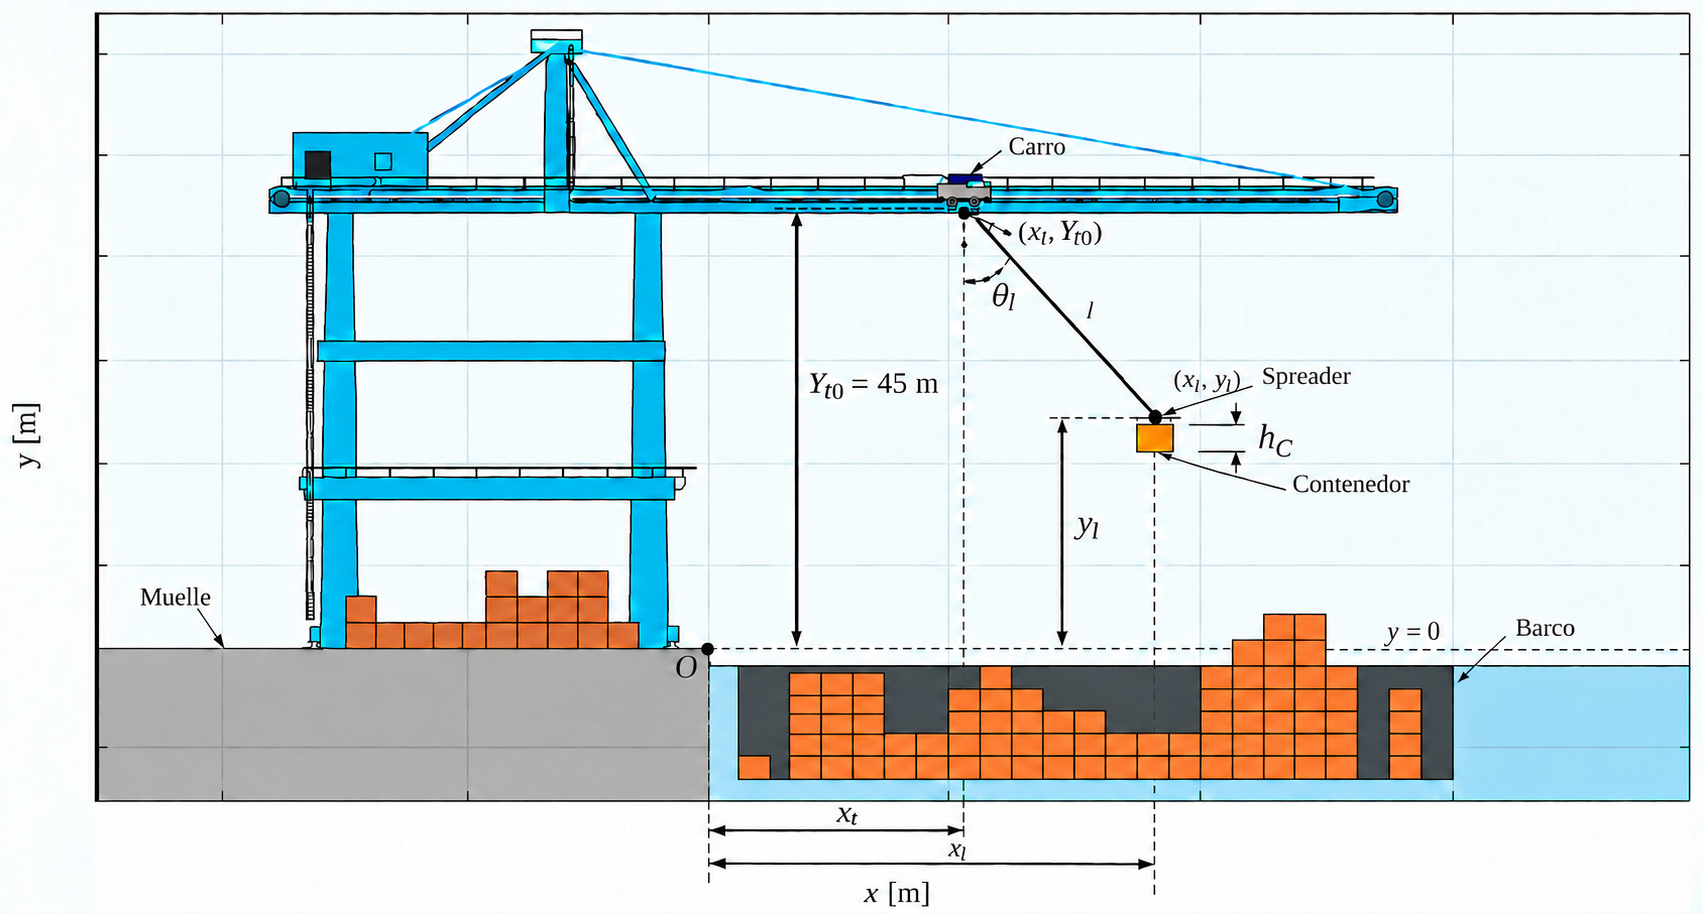
\includegraphics[width=.98\linewidth,height=5.55cm,keepaspectratio]{imagenes/r_003.png}\end{center}\vspace{-1mm}\figcaption{Carro: $x_t$. Centro de la base del spreader: $(x_l,y_l)$. $x$ hacia el barco; $y$ hacia arriba.}
\note{Señalar cada coordenada y distinguir la longitud geométrica de la longitud impuesta por el tambor. La base del contenedor queda una altura Hc por debajo del spreader.}
\end{frame}
\begin{frame}[t,label=slide8]{Carga suspendida y cable de izaje}
\vspace*{-3mm}
\small\setlength{\abovedisplayskip}{4pt}\setlength{\belowdisplayskip}{1pt}
\textbf{Geometría y balances de la carga}
\[
l=\sqrt{(x_l-x_t)^2+(45-y_l)^2},\qquad
\theta_l=\operatorname{atan2}(x_l-x_t,45-y_l)
\]
\[
\begin{aligned}
m_l\ddot x_l&=-2F_{hw}\sin\theta_l+F_{cx},&
m_l\ddot y_l&=2F_{hw}\cos\theta_l+F_{cy}-m_lg
\end{aligned}
\]
\textbf{Cable de izaje y aparejo}
\[
F_{hw}=\begin{cases}
2K_{hw}(l_h)(l-l_h)+2b_{hw}(l_h)(\dot l-\dot l_h),&\text{cable tenso},\\
0,&\text{cable flojo}
\end{cases}
\]
\[
K_{hw}=\frac{236\times10^6}{2l_h+110},\quad b_{hw}=150(2l_h+110),\quad
y_h=45-l_h,\quad 2\dot y_h=r_{hd}\omega_{hd}
\]
\figcaption{$m_l=M_s$ en vacío; $m_l=M_s+M_c$ con contenedor. El cable sólo transmite tracción.}
\note{Se reúnen la geometría, los balances y la tensión del cable. El factor dos corresponde al aparejo equivalente. La conmutación de cable flojo mantiene la ley física de tracción; no usar una rama compresiva.}
\end{frame}
\begin{frame}[t,label=slide10]{Contacto y transmisión del carro}
\small\setlength{\abovedisplayskip}{5pt}\setlength{\belowdisplayskip}{5pt}
\textbf{Contacto con el perfil y cambios de carga}
\[
\delta=y_{obs}-(y_l-h_c),\qquad
\begin{cases}
F_{cy}=K_{cy}\delta-b_{cy}\dot y_l,\quad F_{cx}=-b_{cx}\dot x_l,&\delta\geq0,\\
F_{cx}=F_{cy}=0,&\delta<0
\end{cases}
\]
\figcaption{Toma: $m_l=M_s+M_c$ y perfil de origen $-H_c$. Entrega: $m_l=M_s$ y perfil de destino $+H_c$, con $H_c=2,59$ m.}
\vspace{3mm}\textbf{Transmisión flexible y balance del carro}
\[
F_{tw}=K_{tw}(x_{td}-x_t)+b_{tw}(\dot x_{td}-\dot x_t)
\]
\[
M_t\ddot x_t+b_t\dot x_t=F_{tw}+2F_{hw}\sin\theta_l
\]
\figcaption{$M_t=30\,000$ kg; $K_{tw}=480$ kN/m; $b_{tw}=3$ kN s/m. El desplazamiento del tambor $x_{td}$ puede diferir del carro físico $x_t$.}
\note{El contacto y los twistlocks determinan los eventos de toma y entrega. El cable flexible explica la diferencia entre la medición del accionamiento y la posición real del carro.}
\end{frame}
\begin{frame}[t,label=slide12]{Accionamientos: límite y dinámica de torque}
\relax\setlength{\parskip}{0pt}\small
\begin{center}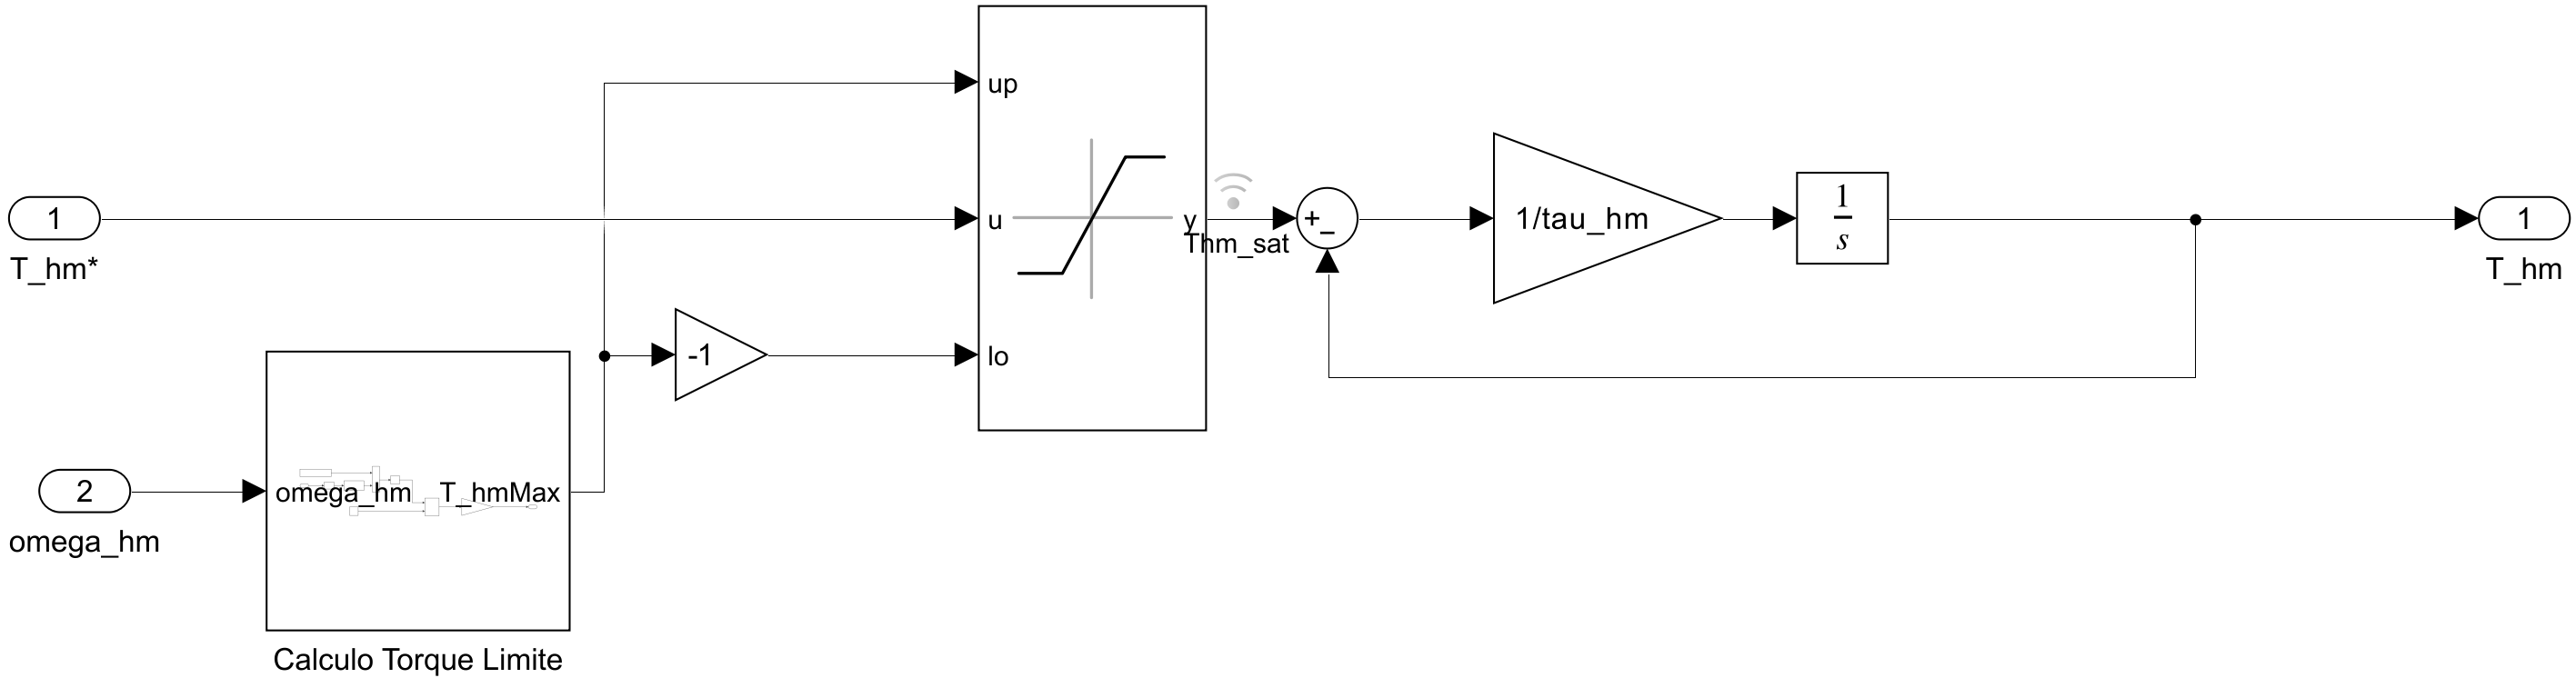
\includegraphics[width=\linewidth,height=3.1cm,keepaspectratio]{imagenes/modulador_torque_izaje_20261012.png}\end{center}
\[
T_{m,\mathrm{lim}}^*=\operatorname{sat}_{T_{\max}(\omega_m)}(T_m^*),\qquad
\tau_m\dot T_m+T_m=T_{m,\mathrm{lim}}^*,\quad \tau_m=1\ \mathrm{ms}
\]
\figcaption{Consigna solicitada $T_m^*$ $\to$ límite según velocidad $\to$ torque aplicado $T_m$. La capacidad disminuye por encima de la velocidad nominal.}
\note{Captura del modulador real de Simulink. La saturación dinámica precede al primer orden. Los permisos y los frenos actúan por separado.}
\end{frame}
\begin{frame}[t,label=accionamientosparametros]{Accionamientos y frenos: balances y parámetros}
\small\setlength{\parskip}{0pt}\setlength{\abovedisplayskip}{4pt}\setlength{\belowdisplayskip}{4pt}
\[
\begin{aligned}
J_t\dot\omega_{td}+b_d\omega_{td}&=i_t(T_{tm}+T_{tb})-r_{td}F_{tw},\\
J_h\dot\omega_{hd}+b_h\omega_{hd}&=i_h(T_{hm}+T_{hb})+T_{hEb}-r_{hd}F_{hw}
\end{aligned}
\]
\begin{center}\renewcommand{\arraystretch}{1.05}
\begin{tabular}{lrr}\toprule
Parámetro & Carro & Izaje\\\midrule
Radio de tambor [m] & 0,50 & 0,75\\
Reducción $i$ & 30 & 22\\
Torque nominal motor [kN m] & 4 & 20\\
Freno de operación [kN m] & 5 & 50\\
Freno de emergencia, eje lento [kN m] & --- & 1100\\\bottomrule
\end{tabular}\end{center}
\figcaption{El freno aplicado se opone a la rotación, con torque limitado; abierto, su torque es cero. El freno de operación actúa en el motor y el de emergencia en el eje lento.}
\note{Las inercias y pérdidas se reflejan al eje del tambor. El torque del freno de operación se multiplica por la reducción; el de emergencia de izaje actúa directamente. La regulación nominal se deduce con frenos abiertos. La secuencia de apertura y cierre se desarrolla en el supervisor.}
\end{frame}
\begin{frame}[t,label=plantacarro]{Planta Simulink: accionamiento y cable del carro}
\relax
\figurefooter{El torque mueve el tambor. El cable elástico transmite fuerza al carro físico.}
\vspace{-2mm}\makebox[\linewidth][c]{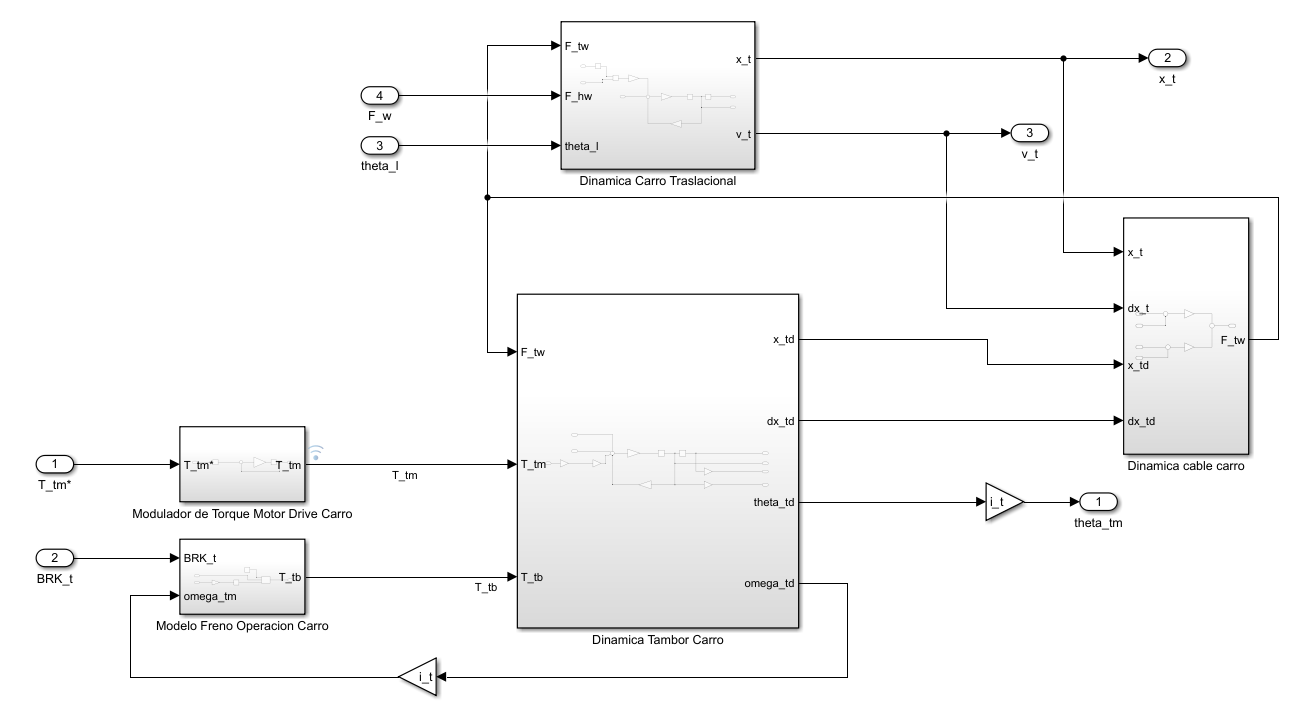
\includegraphics[width=15.0cm,height=6.05cm,keepaspectratio,trim=18.00bp 4.20bp 9.60bp 9.60bp,clip]{imagenes/P_carro1.png}}\par\note{Recorrer torque motor, inercia del accionamiento, desplazamiento equivalente del tambor, deformación del cable y balance del carro. Las posiciones del encoder y del carro físico no son intercambiables.}
\end{frame}


\begin{frame}[t,label=slide13]{Encoders y señales: implementación en Simulink}
\relax
\figurefooter{Encoders, ángulo y velocidad angular, tensión filtrada con $G_F(s)=1/(0{,}1s+1)$ y protecciones. Sin ruido ni cuantización añadidos.}
\vspace{-2mm}\makebox[\linewidth][c]{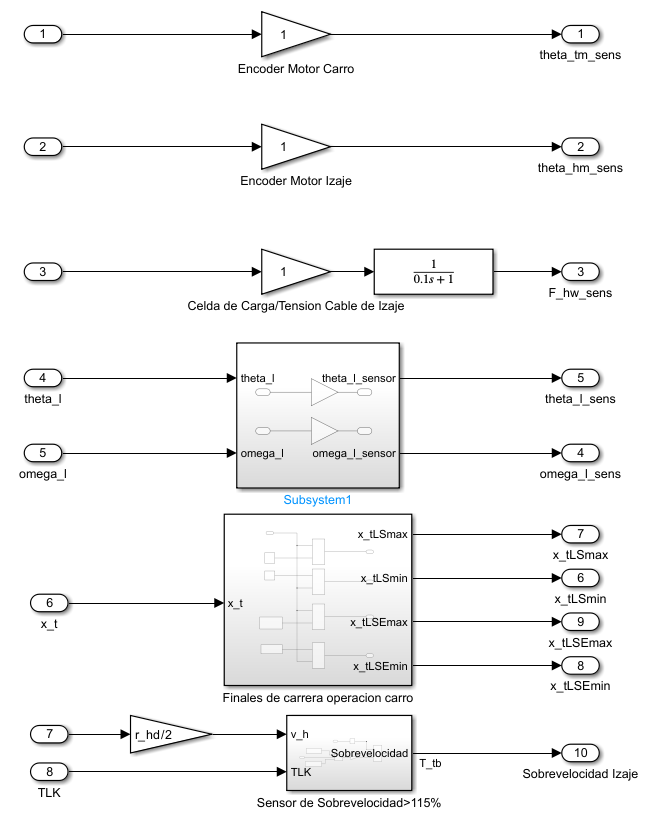
\includegraphics[width=15.0cm,height=6.05cm,keepaspectratio,trim=8.40bp 1.80bp 4.20bp 3.60bp,clip]{imagenes/Sens_1.png}}\par\note{Captura original del informe v3, subsistema SENSORES. Los encoders entregan ángulo del motor. Los estimadores convierten esa lectura en velocidad, manteniendo el radio, la transmisión y el factor 2 del izaje.}
\end{frame}


\begin{frame}[t,label=slide14]{Perfil relevado y reconocimiento de carga}
\begin{columns}[T,onlytextwidth]
\column{0.49\textwidth}\textbf{Toma confirmada}\[
M_s\longrightarrow M_s+M_c
\]
Perfil de origen: $-H_c$.\par\vspace{6mm}\textbf{Entrega confirmada}\[
M_s+M_c\longrightarrow M_s
\]
Perfil de destino: $+H_c$.
\column{0.47\textwidth}\begin{itemize}
\item El LIDAR mide con un desplazamiento de 3 m respecto del carro.
\item El perfil disponible se construye durante el barrido.
\item PICK / PLACE reconoce toma, apoyo y liberación.
\item El supervisor trabaja con el perfil actualizado.
\end{itemize}
\end{columns}
\note{Explicar que la escena física y el perfil relevado no son lo mismo. Las pruebas completas incluyen barrido real; el ensayo de productividad comienza con perfil conocido.}
\end{frame}
\begin{frame}[t,label=pickchart]{PICK/PLACE: estados de reconocimiento en Simulink}
\relax
\vspace{-2mm}\makebox[\linewidth][c]{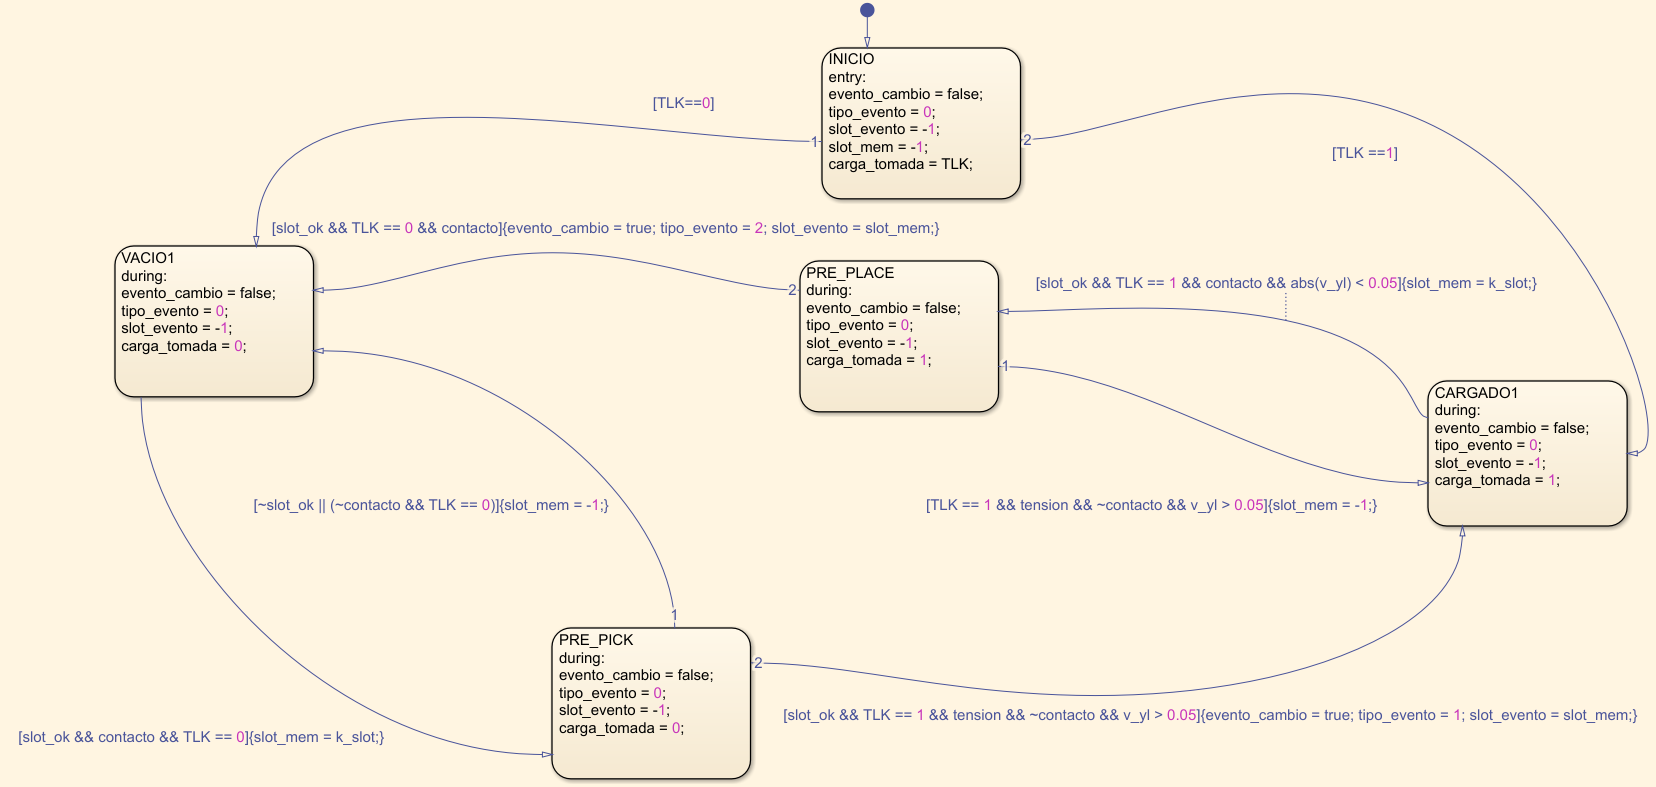
\includegraphics[width=15.0cm,height=5.0cm,keepaspectratio,trim=8.40bp 0.00bp 1.20bp 0.00bp,clip]{imagenes/PickPlace_chart.png}}\par\vspace{1mm}{\fontsize{8}{9.4}\selectfont \texttt{PRE\_PICK} memoriza el slot de origen. Cierre, tensión, pérdida de contacto y ascenso confirman la toma. \texttt{PRE\_PLACE} memoriza el apoyo. Apertura de twistlocks con contacto confirma la entrega.}
\note{VACIO1 y CARGADO1 representan la asociación de la carga. Las condiciones de contacto y tensión usan histéresis. Un contacto momentáneo no confirma por sí solo la transferencia. El evento lleva el slot memorizado y se emite una vez.}
\end{frame}
\begin{frame}[t,label=pickperfil]{PICK/PLACE: evento y actualización del perfil}
\relax
\vspace{-2mm}\makebox[\linewidth][c]{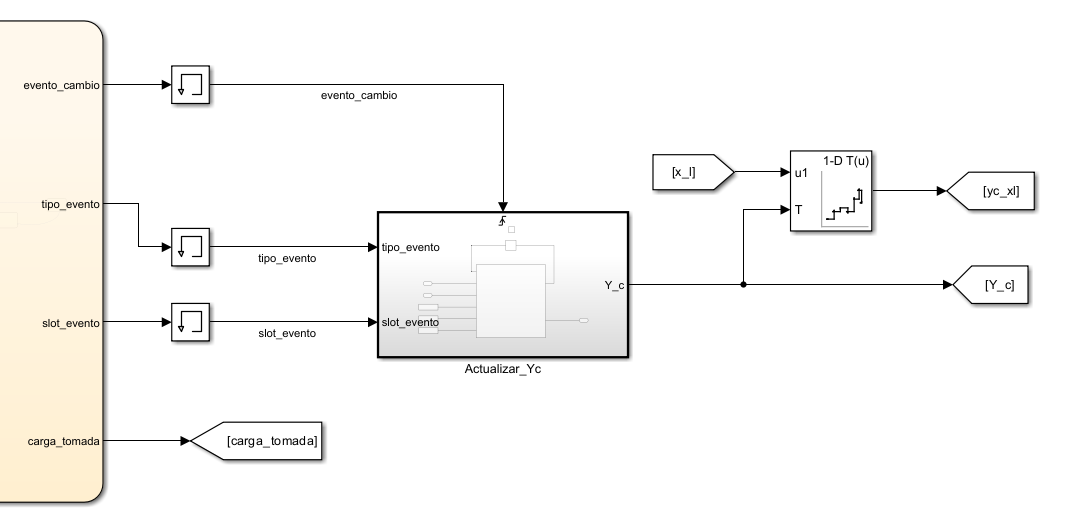
\includegraphics[width=15.0cm,height=4.05cm,keepaspectratio,trim=0.00bp 3.00bp 16.80bp 9.00bp,clip]{imagenes/PickPlace_actObs.png}}\par
{\fontsize{9}{10.5}\selectfont
\[
n_k^+=\begin{cases}\max(n_k-1,0),&\text{toma},\\n_k+1,&\text{entrega},\end{cases}\quad
Y_c(k)=Z_{base}(k)+n_k^+H_c
\]
}
\figcaption{El pulso habilita la actualización de un slot válido y no bloqueado. Las memorias separan reconocimiento, actualización y consulta espacial del contacto.}
\note{El evento tiene tipo_evento y slot_evento. El perfil físico actualizado vuelve al modelo de contacto y al LIDAR simulado. Distinguirlo del perfil relevado almacenado por el supervisor.}
\end{frame}


\section{Diseño del control regulatorio}
\begin{frame}[plain,label=seccion2]
\setbeamertemplate{frametitle}{}
\vfill
{\fontsize{25}{29}\selectfont\bfseries Diseño del control regulatorio\par}
\vspace{4mm}\textcolor{accent}{\rule{.75\linewidth}{1pt}}\par\vspace{3mm}
{\large Modelos reducidos, cascadas y amortiguamiento del balanceo.\par}\vfill
\note{Ubicar este bloque en el recorrido y anunciar su objetivo.}
\end{frame}
\begin{frame}[t,label=slide15]{Regulación de carro e izaje}
\relax
\figurefooter{Referencias de posición, velocidad y aceleración; corrección anti-sway y compensación de fuerzas.}
\vspace{-2mm}\makebox[\linewidth][c]{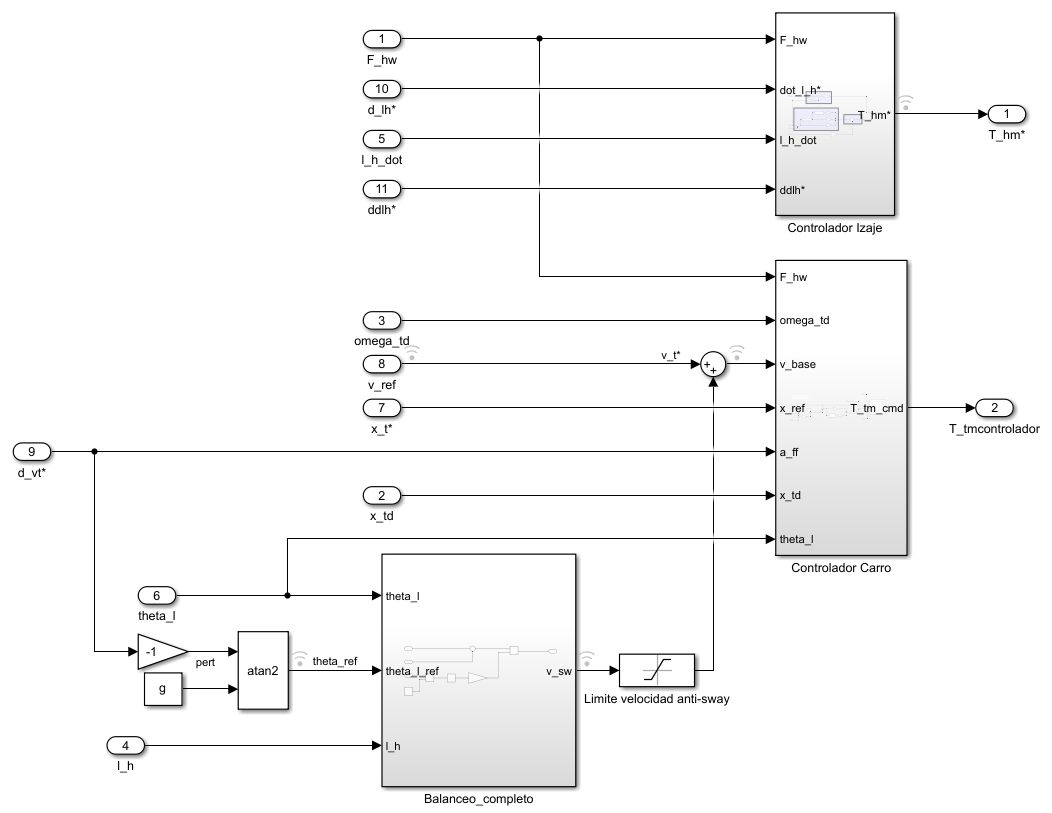
\includegraphics[width=15.0cm,height=6.05cm,keepaspectratio,trim=7.00bp 2.00bp 7.00bp 7.00bp,clip]{imagenes/r_015.png}}\par\note{Recorrer el diagrama una sola vez. El supervisor genera consignas y el regulador convierte referencias y mediciones en torque.}
\end{frame}
\begin{frame}[t,label=slide16]{Carro: modelo reducido y compensación de torque}
\vspace*{-3mm}
\small\setlength{\abovedisplayskip}{4pt}\setlength{\belowdisplayskip}{4pt}
\[
\begin{aligned}
M_t\ddot x_t+b_t\dot x_t&=F_{tw}+2F_{hw}\sin\theta_l,\\
\frac{J_t}{r_{td}^2}\ddot x_{td}+\frac{b_d}{r_{td}^2}\dot x_{td}
&=\frac{i_t}{r_{td}}(T_{tm}+T_{tb})-F_{tw}
\end{aligned}
\]
Con $x_t\simeq x_{td}$:
\[
M_{EQt}\ddot x_t+b_{EQt}\dot x_t=\frac{i_t}{r_{td}}(T_{tm}+T_{tb})+2F_{hw}\sin\theta_l
\]
Con freno abierto, $T_{tb}=0$:
\[
T_{tm}^*=\frac{r_{td}M_{EQt}}{i_t}
\left(a_{cmd}+\frac{b_{EQt}}{M_{EQt}}\hat v_t
-\frac{2F_{hw}}{M_{EQt}}\sin\theta_l\right)
\]
\[
\boxed{\ddot x_t\simeq a_{cmd},\qquad \frac{V(s)}{A_{cmd}(s)}\simeq\frac1s}
\]
\figcaption{Equivalencia nominal con transmisión rígida, estimación de velocidad y torque disponible.}
\note{Los parámetros equivalentes agrupan la masa y las pérdidas del carro con las inercias y rozamientos reflejados del accionamiento. Su desarrollo permanece en el informe. La compensación de la reacción horizontal permanece activa aunque se deshabilite la corrección anti-sway.}
\end{frame}
\begin{frame}[t,label=slide17]{Carro: cascada y ecuaciones de los lazos}
\relax\setlength{\parskip}{0pt}
\vspace{-2mm}{\centering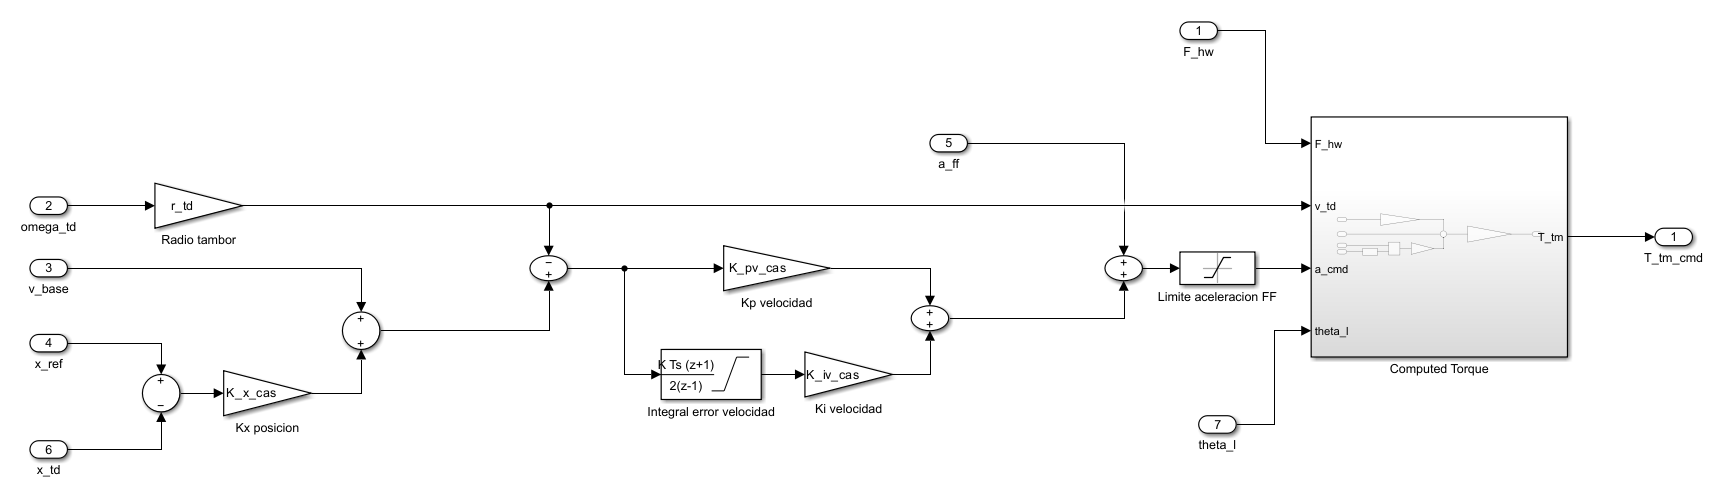
\includegraphics[width=15cm,height=3.55cm,keepaspectratio]{imagenes/CR_carro_cascada_sin_antiwindup.png}\par}
\vspace{-1mm}
\begin{columns}[T,onlytextwidth]
\column{.48\textwidth}\fontsize{9.5}{11}\selectfont
\setlength{\abovedisplayskip}{2pt}\setlength{\belowdisplayskip}{2pt}
\[e_x=x_{ref}-\hat x_t\]
\[v_c=v_{ref}+K_xe_x+v_{sw}\]
\[e_v=v_c-\hat v_t,\qquad\dot I_v=e_v\]
\column{.48\textwidth}\fontsize{9.5}{11}\selectfont
\setlength{\abovedisplayskip}{2pt}\setlength{\belowdisplayskip}{2pt}
\[a_u=a_{ref}+K_{pv}e_v+K_{iv}I_v\]
\[a_c=\operatorname{sat}_{a_{max}}(a_u)\]
\figcaption{Posición $\to$ velocidad $\to$ aceleración $\to$ torque.}
\end{columns}
{\small\setlength{\abovedisplayskip}{2pt}\setlength{\belowdisplayskip}{2pt}
\[\boxed{T_{tm}^*=\frac{r_{td}}{i_t}\left(M_{EQt}a_c+b_{EQt}\hat v_t-2F_w\sin\theta_l\right)}\]}
\figurefooter{Captura del controlador sin anti-windup. Compensación mecánica hasta torque.}
\note{Captura final aportada por el usuario: cascada base sin anti-windup. La suma de referencia de velocidad, corrección de posición y anti-sway forma vc sin saturación de velocidad en esta versión. El PI produce aceleración, se suma a_ff y se limita la aceleración total antes de Computed Torque. El rótulo Limite aceleracion FF limita la suma completa, no sólo el término anticipativo. La formulación se ajustó a esta captura; el MC final y sus límites permanecen como se desarrollan posteriormente. v_base reúne las referencias comunes; swTransfer continúa pendiente. No se modificó el SLX ni el código.}
\end{frame}
\begin{frame}[t,label=gv]{Carro: transferencia y polos de la cascada}
\fontsize{10}{11.5}\selectfont
\setlength{\abovedisplayskip}{3pt}\setlength{\belowdisplayskip}{3pt}
Para estudiar el lazo interior: $a_{ref}=0$, $v_{sw}=0$ y condiciones iniciales nulas; sin límites activos.
\[
sV=A_{cmd},\qquad A_{cmd}=\left(K_{pv}+\frac{K_{iv}}s\right)(V_c-V)
\]
\[
(s^2+K_{pv}s+K_{iv})V=(K_{pv}s+K_{iv})V_c,\qquad
\boxed{G_v(s)=\frac{V}{V_c}=\frac{K_{pv}s+K_{iv}}{s^2+K_{pv}s+K_{iv}}}
\]
\[
P_v(s)=(s-p_f)(s-p_i),\quad K_{pv}=-(p_f+p_i),\quad K_{iv}=p_fp_i
\]
\[
K_{pv}=2,4\ \mathrm{s^{-1}},\quad K_{iv}=0,2\ \mathrm{s^{-2}}
\quad\Rightarrow\quad p_f=-2,314,\quad p_i=-0,0864\ \mathrm{s^{-1}}
\]
\[
\text{Cero de }G_v:\quad -K_{iv}/K_{pv}=-0,0833\ \mathrm{s^{-1}}
\]
\[
1+\frac{K_xG_v(s)}s=0\quad\Rightarrow\quad
P_{xv}(s)=s^3+K_{pv}s^2+(K_{iv}+K_xK_{pv})s+K_xK_{iv}
\]
\note{La planta nominal compensada es un integrador. La cascada de posición tiene un polinomio cúbico. Los polos no corresponden a la planta flexible completa.}
\end{frame}

\begin{frame}[t,label=poloscascada]{Carro: polos y cero de los modelos nominales}
\relax
\begin{center}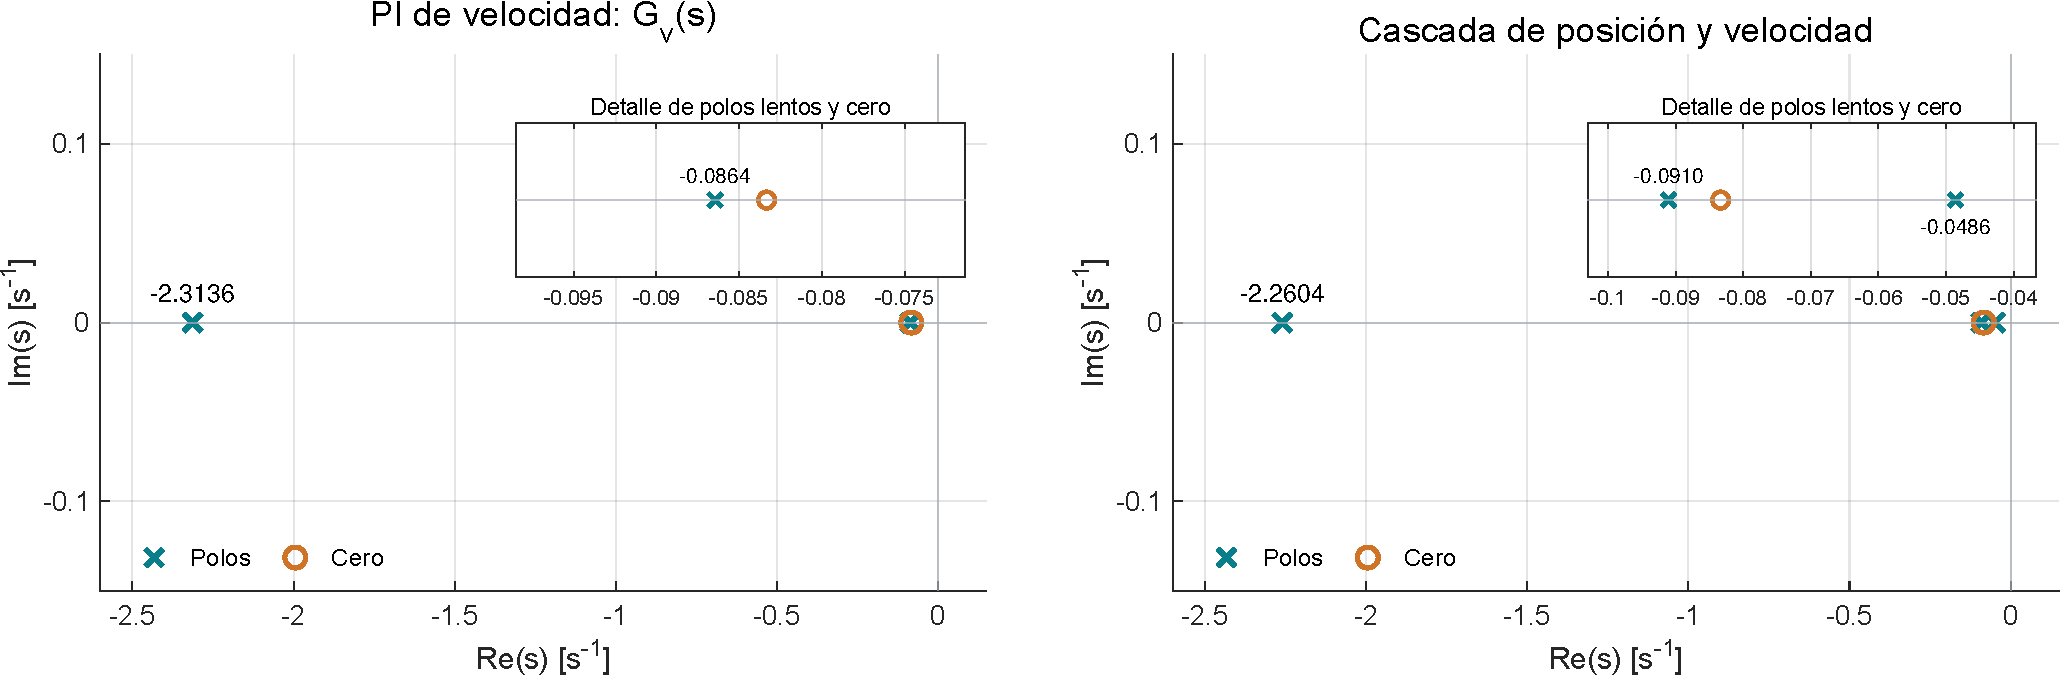
\includegraphics[width=\linewidth,height=4.6cm,keepaspectratio]{imagenes/polos_carro_nominales_20261012.pdf}\end{center}
\vspace{-3mm}\small
\[K_x=0{,}05\ \mathrm{s^{-1}},\quad K_{pv}=2{,}4\ \mathrm{s^{-1}},\quad K_{iv}=0{,}2\ \mathrm{s^{-2}}\]
\figcaption{Cruces: polos. Círculo: cero $z=-K_{iv}/K_{pv}=-0{,}0833\ \mathrm{s^{-1}}$. Modelos reducidos sin saturación; el péndulo y la flexibilidad no están incluidos.}
\note{Los puntos se recalcularon a partir de los polinomios del PI y de la cascada completa con las ganancias base. El detalle ampliado evita confundir el polo lento con el cero próximo. La cascada tiene tres polos; no se obtiene agregando exactamente -Kx a los polos interiores. La figura no representa la sintonía productiva final ni polos identificados de la planta flexible.}
\end{frame}
\begin{frame}[t,label=gananciasversiones]{Carro: sintonías y alcance de la asignación}
\begin{center}\small
\begin{tabular}{lrrr}\toprule
Configuración & $K_x$ [s$^{-1}$] & $K_{pv}$ [s$^{-1}$] & $K_{iv}$ [s$^{-2}$]\\\midrule
Ensayos aislados & 0,05 & 2,40 & 0,20\\
Ciclo integrado inicial & 0,20 & 2,40 & 0,20\\
Ciclo productivo ajustado & 0,25 & 3,20 & 0,267\\\bottomrule
\end{tabular}\end{center}
\begin{itemize}
\item La asignación nominal orienta el diseño. Cada configuración requiere comprobar seguimiento y balanceo con la planta completa.
\item Los cambios de ganancias del ajuste productivo pertenecen a otro ensayo.
\item Manual y automático comparten regulación dentro de la misma configuración.
\end{itemize}
\note{Valores documentados en el informe v3 y en la presentación original. No atribuir las métricas de una corrida a otra sintonía.}
\end{frame}


\begin{frame}[t,label=slide19]{Carro y péndulo: modelo y referencia angular}
\relax\setlength{\parskip}{0pt}
\begin{columns}[T,onlytextwidth]
\column{.39\textwidth}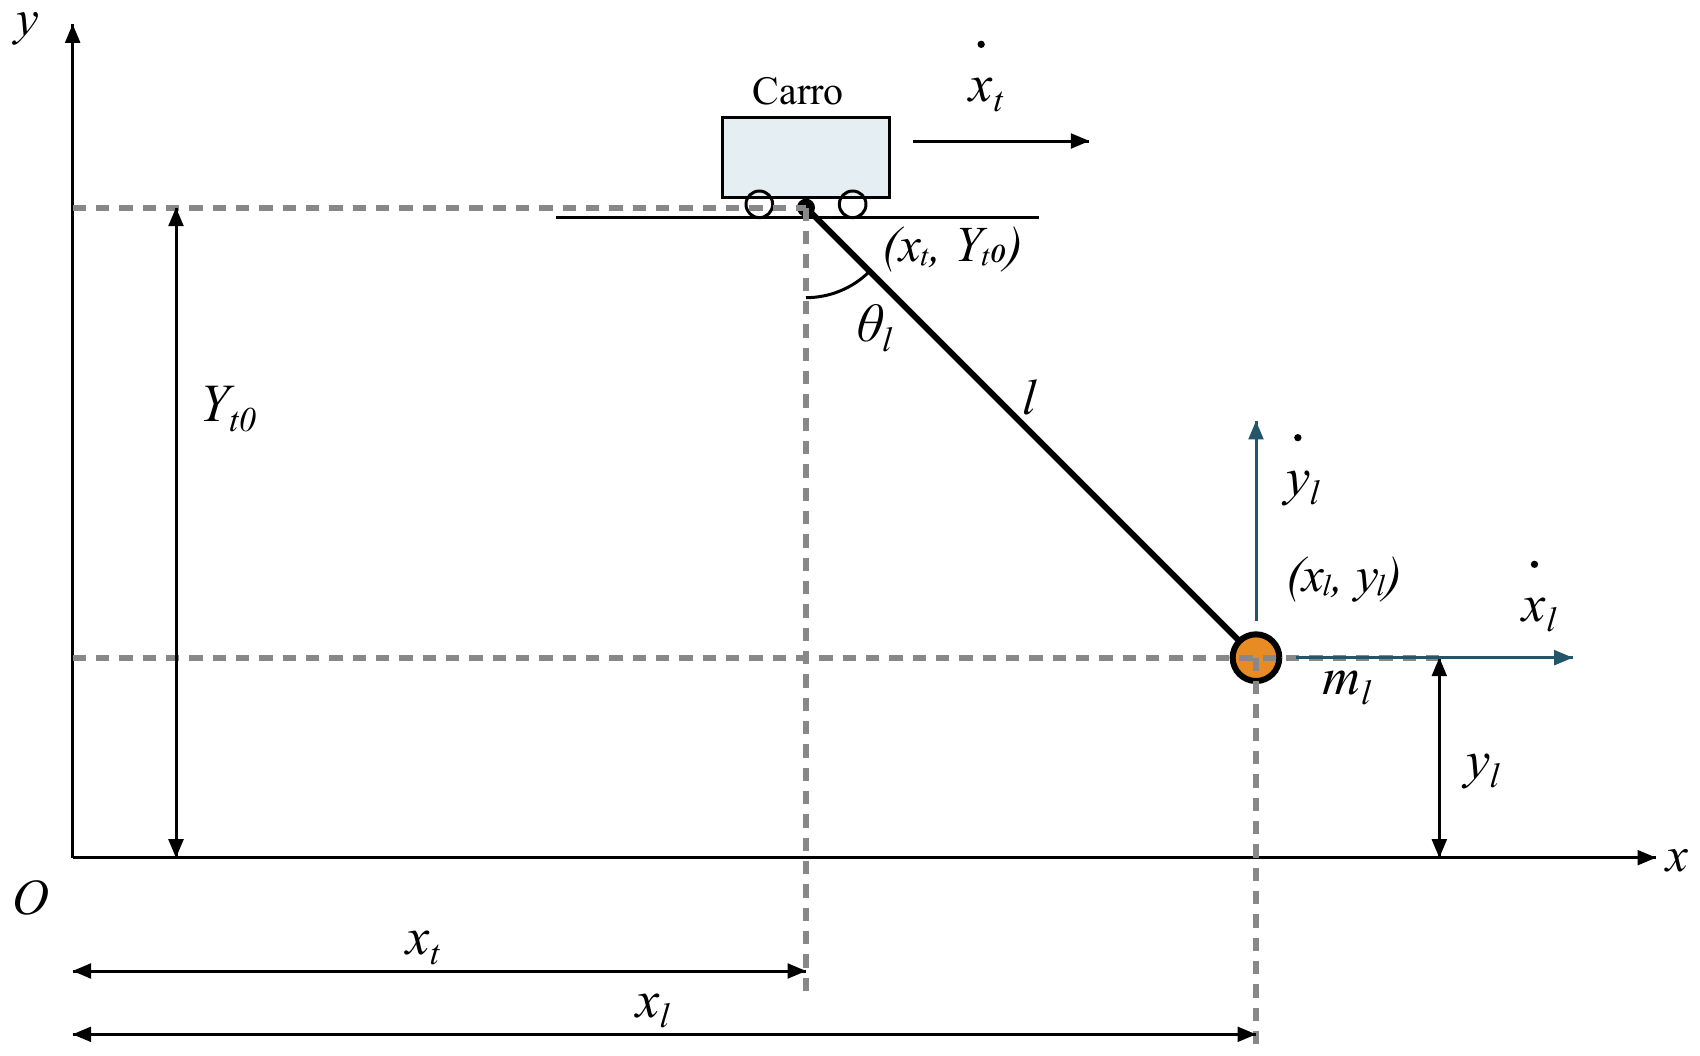
\includegraphics[width=\linewidth,height=3.6cm,keepaspectratio]{imagenes/r_018.png}\par
\figcaption{$\theta_l>0$: carga hacia $+x$. La aceleración positiva inclina el equilibrio hacia $-x$.}
\column{.58\textwidth}\small
\setlength{\abovedisplayskip}{4pt}\setlength{\belowdisplayskip}{4pt}\setlength{\abovedisplayshortskip}{0pt}\setlength{\belowdisplayshortskip}{4pt}
\textbf{Modelo aproximado del péndulo}
\[\boxed{\ddot\theta_l+\omega_p^2\theta_l=-\frac{\ddot x_t}{l}},\qquad\omega_p=\sqrt{\frac gl}\]
\textbf{Equilibrio bajo aceleración}
\[\theta_{ref}\simeq-\frac{a_{ref}}g\]
\figcaption{Implementación: $\theta_{ref}=\operatorname{atan2}(-a_{ref},g)$.}
\[\boxed{e_\theta=\theta_l-\theta_{ref}}\]
\end{columns}
\vspace{1mm}\small La aceleración excita el péndulo. Se busca reducir el balanceo alrededor del equilibrio angular.
\par\vspace{1mm}\figcaption{Diseño: ángulo pequeño y longitud aproximadamente constante. Deducción no lineal en respaldo.}
\note{Partir de la ecuación aproximada con longitud constante y explicar su entrada: la aceleración horizontal del apoyo. Para aceleración constante, el equilibrio satisface (g/l) theta_ref=-a_ref/l, de donde theta_ref=-a_ref/g. La implementación utiliza atan2 para representar la inclinación de equilibrio; se linealiza sólo para la deducción. El error angular es la desviación respecto de ese equilibrio, que es cero cuando la referencia de aceleración es cero. La ecuación completa con 2 dot l dot theta y geometría no lineal queda en las diapositivas de respaldo. Distinguir longitud geométrica l y longitud inferida lh.}
\end{frame}
\begin{frame}[t,label=antiswaydiseno]{Anti-sway: cómo aparece el amortiguamiento}
\relax\setlength{\parskip}{0pt}
\small\setlength{\abovedisplayskip}{2pt}\setlength{\belowdisplayskip}{2pt}
\textbf{1. Corrección de velocidad proporcional al error angular}
\[\boxed{v_{sw}=k_{sw}e_\theta}\]
\textbf{2. Efecto sobre la aceleración del carro}
\[\dot x_t\simeq v_{ref}+k_{sw}e_\theta
\quad\Longrightarrow\quad
\ddot x_t\simeq a_{ref}+k_{sw}\dot e_\theta\]
\textbf{3. Sustitución en el péndulo, con $\theta_l=e_\theta+\theta_{ref}$}
\[\boxed{\ddot e_\theta+
\underbrace{\textcolor{accent}{\frac{k_{sw}}{l}\dot e_\theta}}_{\text{amortiguamiento introducido}}
+\omega_p^2e_\theta\simeq0}\]
\par\vspace{2mm}\textcolor{accent}{La corrección de velocidad introduce amortiguamiento a través de la aceleración del carro.}
\par\vspace{2mm}\figcaption{Diseño nominal: ganancia y longitud constantes, referencia angular casi constante y buen seguimiento de velocidad.}
\note{Seguir la cadena e_theta -> v_sw -> aceleración del carro -> amortiguamiento. Derivar la velocidad con ksw constante genera ksw dot e_theta. Al sustituir en la ecuación del péndulo: theta_ddot+(ksw/l) e_theta_dot+(g/l) theta=-a_ref/l. Reemplazar theta=e_theta+theta_ref produce en el lado derecho -theta_ref_ddot-(g/l)theta_ref-a_ref/l. La elección theta_ref aproximadamente -a_ref/g cancela los dos términos de equilibrio; queda -theta_ref_ddot. La ecuación homogénea presentada supone que esa excitación es despreciable. Para aislar este mecanismo se omiten la corrección de posición y las saturaciones y se aproxima el seguimiento de velocidad. La realimentación angular crea el término amortiguador a través de la dinámica cinemática del carro; no se impone como una propiedad física original del cable.}
\end{frame}
\begin{frame}[t,label=antiswayscheduling]{Anti-sway: ganancia y adaptación con la longitud}
\relax\setlength{\parskip}{0pt}
\small\setlength{\abovedisplayskip}{4pt}\setlength{\belowdisplayskip}{4pt}
\textbf{Respuesta nominal buscada}
\[\ddot e_\theta+2\zeta_{sw}\omega_p\dot e_\theta+\omega_p^2e_\theta=0\]
\begin{columns}[T,onlytextwidth]
\column{.61\textwidth}\small
\textbf{Comparación del término amortiguador}
\[\frac{k_{sw}}l=2\zeta_{sw}\omega_p
\quad\Longrightarrow\quad k_{sw}=2\zeta_{sw}\sqrt{gl}\]
\textbf{Ganancia actualizada desde el encoder}
\[\boxed{k_{sw}(l_h)=2\zeta_{sw}\sqrt{g\,l_h}}\]
\column{.35\textwidth}\fontsize{9.2}{11}\selectfont
\begin{tabular}{rrr}\toprule
$l_h$ [m] & $\omega_p$ [rad/s] & $k_{sw}$\\\midrule
10 & 0,990 & 19,81\\
20 & 0,700 & 28,01\\
40 & 0,495 & 39,62\\\bottomrule
\end{tabular}\par\vspace{2mm}
\figcaption{$\zeta_{sw}=1$; $k_{sw}$ en m/s por rad. $l_h\simeq l$ para el diseño.}
\end{columns}
\vspace{1mm}\small $\zeta_{sw}$ fija el amortiguamiento nominal. El encoder actualiza la ganancia: \textbf{gain scheduling}.
\par\vspace{1mm}\figcaption{Para $\zeta_{sw}=1$: amortiguamiento crítico nominal. Frecuencia y tiempo de respuesta varían con la longitud.}
\note{Comparar ksw/l, obtenido al cerrar el anti-sway, con el coeficiente deseado 2 zeta_sw omega_p. La elección de ganancia es consecuencia de esa comparación. Para zeta=1 el polinomio nominal es (s+omega_p)^2: amortiguamiento crítico del error angular, no del sistema físico completo. Se utiliza lh obtenido del encoder como aproximación de la longitud geométrica. La tabla usa g=9,80665 m/s2. La adaptación se interpreta congelando localmente la longitud; si cambia rápidamente aparecen los términos asociados a dot l y dot ksw y no se garantiza una razón de amortiguamiento exacta. Los factores de ajuste, habilitación gradual y límites se presentan posteriormente en integración. No se modifica el código de control.}
\end{frame}

\begin{frame}[t,label=slide21]{Izaje: del balance de torque al modelo en longitud}
\vspace*{-3mm}
\small\setlength{\parskip}{0pt}
\setlength{\abovedisplayskip}{3pt}\setlength{\belowdisplayskip}{3pt}
\[
J_h=J_{hd+hEb}+i_h^2J_{hm+hb},\qquad b_h=b_{hd}+i_h^2b_{hm}
\]
\[
J_h\dot\omega_{hd}+b_h\omega_{hd}
=i_h(T_{hm}+T_{hb})+T_{hEb}-r_{hd}F_{hw}
\]
\[
\omega_{hd}=-\frac{2\dot l_h}{r_{hd}},\qquad
M_{EQh}=\frac{2J_h}{r_{hd}^2},\qquad b_{EQh}=\frac{2b_h}{r_{hd}^2}
\]
\[
M_{EQh}\ddot l_h+b_{EQh}\dot l_h
=-\frac{i_h}{r_{hd}}(T_{hm}+T_{hb})-\frac{T_{hEb}}{r_{hd}}+F_{hw}
\]
Con frenos abiertos y compensación de tensión medida:
\[
T_{hm}^*=T'_{hm}+\frac{r_{hd}}{i_h}F_{hw}
\quad\Longrightarrow\quad
\boxed{M_{EQh}\ddot l_h+b_{EQh}\dot l_h=-\frac{i_h}{r_{hd}}T'_{hm}}
\]
\figcaption{Torque positivo: reduce $l_h$ y eleva la carga. El factor 2 proviene del aparejo. Se controla la longitud cinemática; la planta conserva la elasticidad del cable.}
\note{Se reflejan las inercias y pérdidas al tambor, incluyendo los frenos de ambos ejes. De y_h=45-l_h y 2 dot y_h=r_hd omega_hd surge el signo negativo. Sustituir omega en el balance y dividir por menos r_hd produce el modelo en longitud. MEQh representa inercia rotacional en esta coordenada, no simplemente la masa suspendida. Con frenos abiertos, la tensión medida se compensa en el torque; la regulación actúa sobre la longitud cinemática del tambor.}
\end{frame}
\begin{frame}[t,label=izajelazoreal]{Izaje: lazo Simulink y ecuaciones implementadas}
\relax\setlength{\parskip}{0pt}
\vspace{-2mm}\makebox[\linewidth][c]{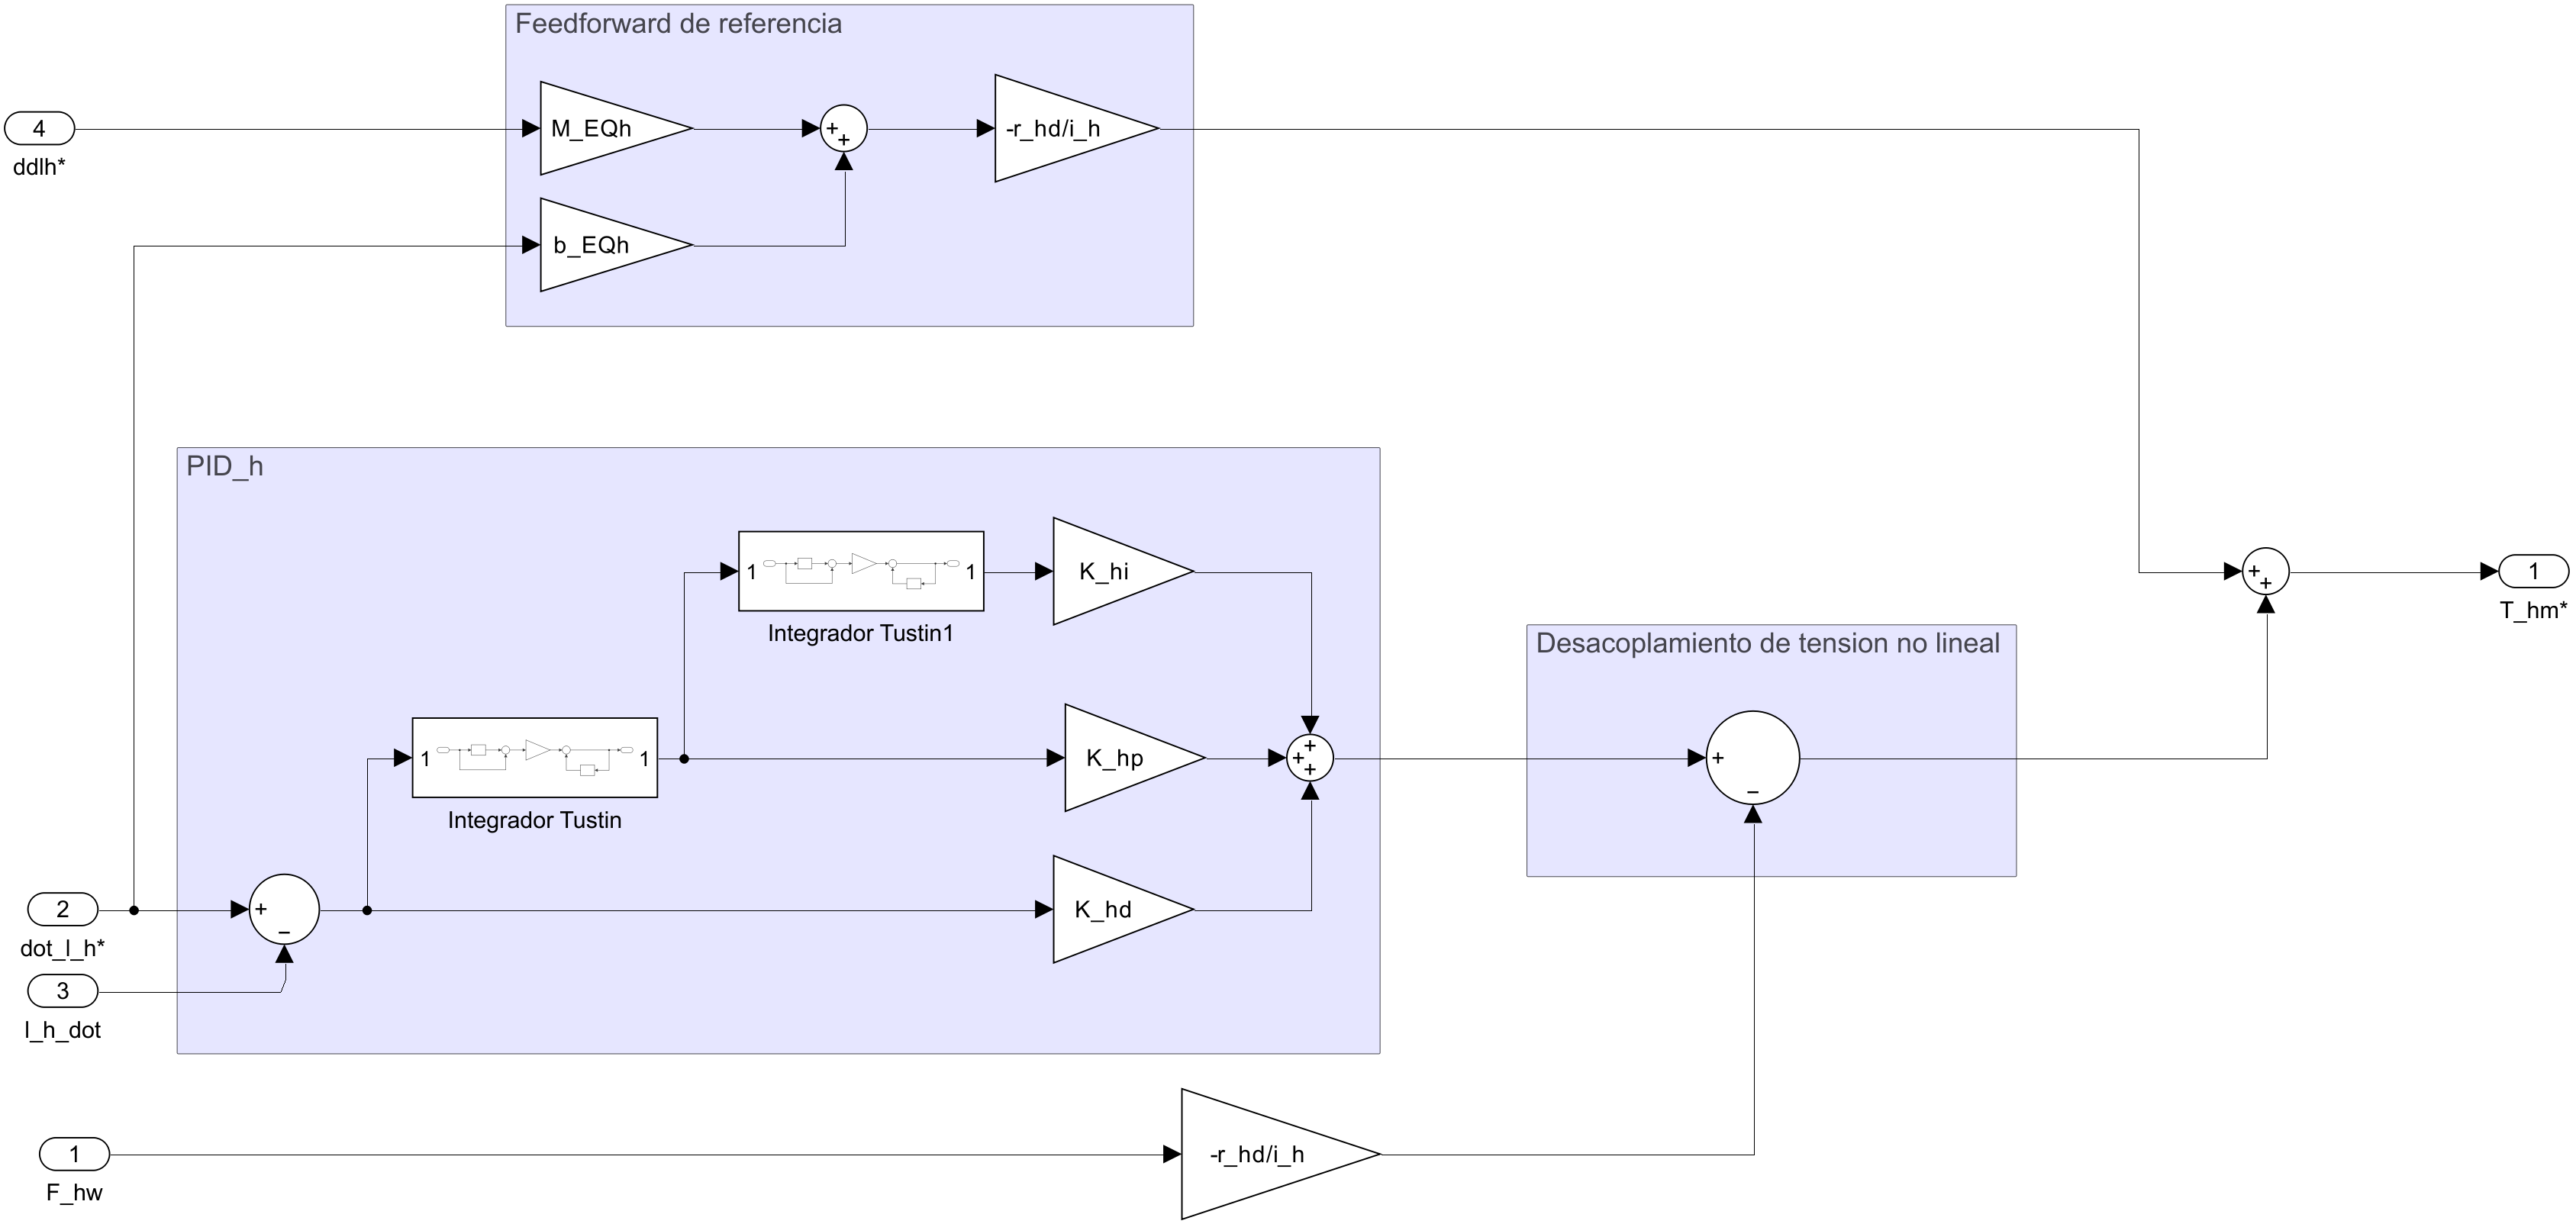
\includegraphics[width=15.0cm,height=4.45cm,keepaspectratio,trim=0.00bp 0.00bp 0.98bp 0.00bp,clip]{imagenes/izaje_lazo_R2.png}}\par\vspace{-2mm}{\small\setlength{\abovedisplayskip}{2pt}\setlength{\belowdisplayskip}{2pt}
\[
e_h=\dot l_h^*-\widehat{\dot l_h},\quad z_1=\int e_h\,dt,\quad z_2=\int z_1\,dt
\]
\[
T_{hm}^*=K_{hd}e_h+K_{hp}z_1+K_{hi}z_2
-\frac{r_{hd}}{i_h}(M_{EQh}\ddot l_h^*+b_{EQh}\dot l_h^*)+\frac{r_{hd}}{i_h}F_{hw}
\]
}\figcaption{La doble integración del error de velocidad equivale al PID de longitud con condiciones iniciales coherentes.}
\note{Captura exportada del modelo R2, contrastada con mc_eje_izaje.m. El MC conserva esta estructura y los signos. No agregar un anti-windup de izaje que no existe en la realización ensayada.}
\end{frame}
\begin{frame}[t,label=izajepolinomio]{Izaje: polinomio cerrado y asignación de ganancias}
\vspace*{-3mm}
\relax
\figurefooter{Las ganancias igualan los coeficientes de $P_d(s)$; la anticipación no modifica los polos nominales.}
\setlength{\parskip}{0pt}
\small\setlength{\abovedisplayskip}{3pt}\setlength{\belowdisplayskip}{3pt}\setlength{\abovedisplayshortskip}{2pt}\setlength{\belowdisplayshortskip}{2pt}
\[
\alpha_h=\frac{i_h}{r_{hd}M_{EQh}},\quad\beta_h=\frac{b_{EQh}}{M_{EQh}},\quad
G_h(s)=-\frac{\alpha_h}{s(s+\beta_h)},\quad C_h(s)=K_{hd}s+K_{hp}+\frac{K_{hi}}s
\]
\[
1+G_hC_h=0\quad\Rightarrow\quad
P_h(s)=s^3+(\beta_h-\alpha_hK_{hd})s^2-\alpha_hK_{hp}s-\alpha_hK_{hi}
\]
\[
P_d(s)=(s+\omega_{posh})(s^2+2\zeta_h\omega_{posh}s+\omega_{posh}^2),\quad n_h=1+2\zeta_h
\]
\[
\begin{aligned}
K_{hp}&=-c_hn_h\omega_{posh}^2,&K_{hi}&=-c_h\omega_{posh}^3,\\
K_{hd}&=\frac{r_{hd}}{i_h}b_{EQh}-c_hn_h\omega_{posh},&c_h&=\frac{r_{hd}M_{EQh}}{i_h}.
\end{aligned}
\]
\vspace{-1mm}\begin{center}\begin{tabular}{lr}\toprule
Diseño & Resultado\\\midrule
$n_h=2,7$, $\omega_{posh}=1,8$ rad/s & $\zeta_h=0,85$\\
Polos nominales & $-1,8$ y $-1,53\pm j\,0,948$\\\bottomrule
\end{tabular}\end{center}
\note{Explicar el signo negativo de la planta: aumentar torque disminuye longitud. La integral agrega el tercer orden. La asignación fija dinámicas del error alrededor de la trayectoria nominal. Presentar el polinomio deseado y el resultado de igualar coeficientes. Mantener las deducciones intermedias para preguntas; los polos pertenecen al modelo reducido.}
\end{frame}



\begin{frame}[t,label=izajepolosfig]{Izaje: diagrama de polos nominales}
\begin{center}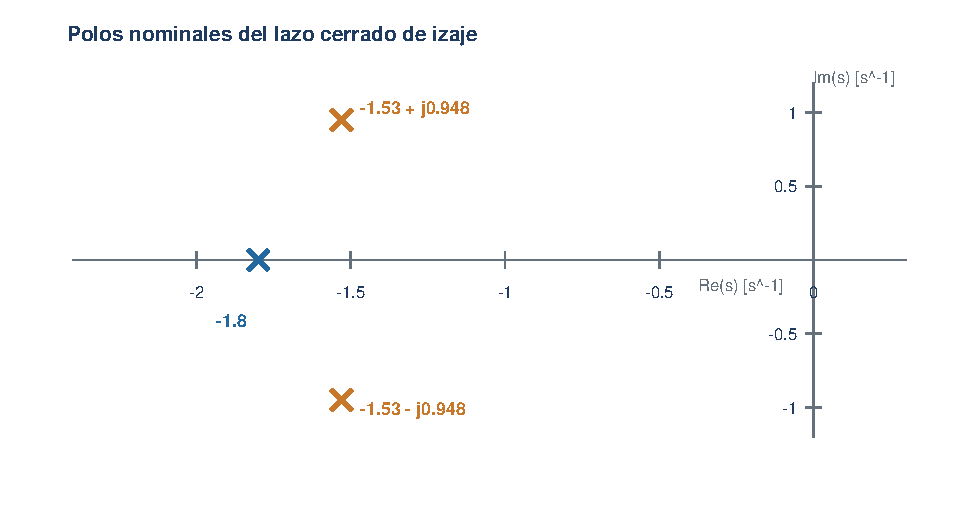
\includegraphics[width=.98\linewidth,height=5.05cm,keepaspectratio]{imagenes/polos_izaje_nominal.pdf}\end{center}\figcaption{Asignación sobre el modelo reducido: un polo real y un par conjugado estable.}
\note{Usar la gráfica del informe y recordar que la tensión filtrada, los límites del drive y el cable elástico no están incluidos en esta asignación.}
\end{frame}



\begin{frame}[t,label=estimadoresencoders]{Observadores continuos de velocidad}
\small\setlength{\parskip}{0pt}
\setlength{\abovedisplayskip}{3pt}\setlength{\belowdisplayskip}{3pt}
Los encoders miden el ángulo del motor. Dos observadores independientes, uno por eje, reconstruyen la velocidad angular del tambor.
\par\vspace{1mm}\textbf{Modelo cinemático de predicción}
\[
u=\frac{\theta_{m,\mathrm{sens}}}{i},\qquad \dot q=\omega,\qquad \dot\omega=0
\]
\begin{columns}[T,onlytextwidth]
\column{.43\textwidth}\small
\setlength{\abovedisplayskip}{2pt}\setlength{\belowdisplayskip}{2pt}\setlength{\abovedisplayshortskip}{2pt}\setlength{\belowdisplayshortskip}{2pt}
\textbf{Observador de Luenberger}
\[
\boxed{\begin{aligned}
\dot{\hat q}&=\hat\omega+l_1(u-\hat q),\\
\dot{\hat\omega}&=l_2(u-\hat q)
\end{aligned}}
\]
\par\vspace{2mm}\figcaption{El ángulo estimado es un estado interno. Las posiciones de los reguladores se calculan directamente desde los encoders.}
\column{.54\textwidth}\small
\setlength{\abovedisplayskip}{2pt}\setlength{\belowdisplayskip}{2pt}\setlength{\abovedisplayshortskip}{2pt}\setlength{\belowdisplayshortskip}{2pt}
\textbf{Asignación de polos}
\[
\begin{aligned}
P_o(s)&=s^2+l_1s+l_2\\
&=s^2+2\zeta_o\omega_os+\omega_o^2
\end{aligned}
\]
\[
\zeta_o=1,\qquad\omega_o=40\ \mathrm{rad/s}
\]
\[
l_1=80\ \mathrm{s^{-1}},\quad l_2=1600\ \mathrm{s^{-2}}
\]
\[
\boxed{p_{o1}=p_{o2}=-40\ \mathrm{s^{-1}}}
\]
\end{columns}
\note{El modelo cinemático es observable: con estados q y omega, A0=[0 1;0 0] y C=[1 0], su matriz de observabilidad es la identidad. La predicción supone velocidad constante; no se impone esa condición al movimiento real. El error entre ángulo medido y estimado corrige ambos estados. Los parámetros coinciden con los observadores continuos del informe, sección 6.2. La realización discreta a 1 ms se explica en las diapositivas del MC.}
\end{frame}
\begin{frame}[t,label=senalesconversion]{Interpretación y conversiones cinemáticas}
\small\setlength{\parskip}{0pt}
\setlength{\abovedisplayskip}{5pt}\setlength{\belowdisplayskip}{5pt}
\textbf{Derivada filtrada y conversiones cinemáticas} (condiciones iniciales nulas):
\[
\frac{\hat\Omega(s)}{U(s)}=s\,\frac{1600}{(s+40)^2},\qquad
\hat v_{td}=r_{td}\hat\omega_{td},\qquad
\widehat{\dot l_h}=-\frac{r_{hd}}{2}\hat\omega_{hd}
\]
A velocidad constante, el error converge a cero. Ante una aceleración angular constante sostenida, una vez extinguido el transitorio:
\[
e_\omega=\omega-\hat\omega=(0,05\ \mathrm{s})\,a_\theta
\]
\figcaption{A bajas frecuencias aproxima la derivada. A altas frecuencias limita la amplificación de las perturbaciones de la medición.}
\note{La transferencia se obtiene al eliminar el estado angular interno con condiciones iniciales nulas. Para una medición ideal, la velocidad estimada respecto de la real sigue 1600/(s+40)^2. El error a aceleración constante es el valor posterior al transitorio, no una igualdad instantánea para cualquier maniobra. Las variables del tambor no deben confundirse con las de la carga o el carro físico cuando interviene la elasticidad.}
\end{frame}
\begin{frame}[t,label=observadoresvalidacion]{Implementación en bloques y validación}
\setlength{\parskip}{0pt}
{\centering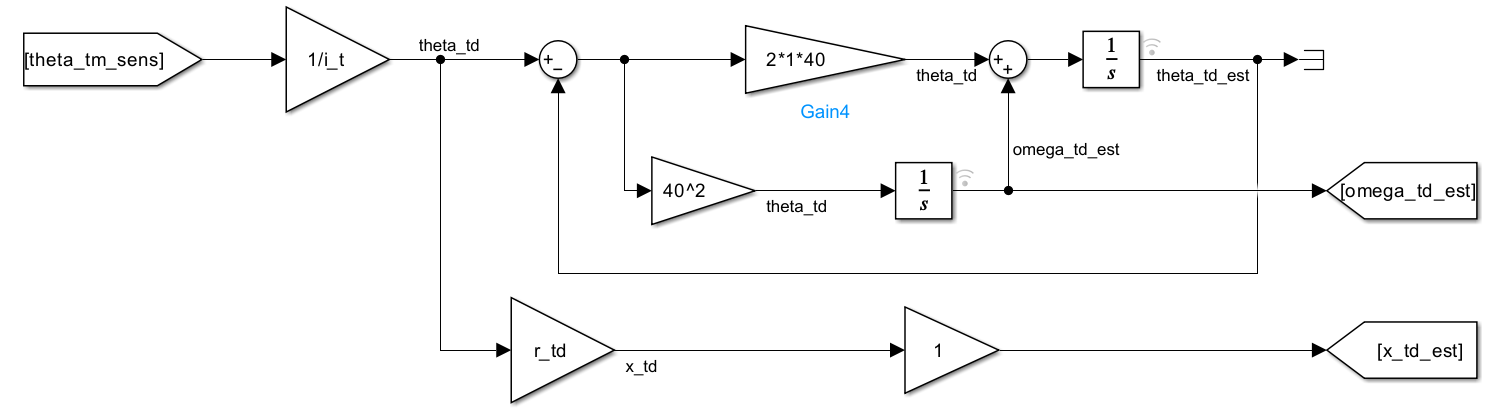
\includegraphics[width=\linewidth,height=2.8cm,keepaspectratio]{imagenes/observador_continuo_carro.png}\par}
\figcaption{Ejemplo: observador continuo del accionamiento del carro y conversión directa de posición desde el encoder.}
\vspace{2mm}
\begin{columns}[T,onlytextwidth]
\column{.50\textwidth}\fontsize{9.5}{11}\selectfont
\textbf{Verificación con ambos ejes en movimiento}\par
Se reprodujeron los registros de los encoders y se compararon las estimaciones con las velocidades de los accionamientos de la planta simulada.
\column{.47\textwidth}\fontsize{9}{10.5}\selectfont
\renewcommand{\arraystretch}{1.05}\setlength{\tabcolsep}{3pt}
\begin{tabular}{@{}lrr@{}}\toprule
Accionamiento & Error RMS & Máx. absoluto\\
& [m/s] & [m/s]\\\midrule
Carro & 0,00540 & 0,02957\\
Izaje & 0,00682 & 0,10548\\\bottomrule
\end{tabular}
\end{columns}\vspace{2mm}
\figcaption{Buen seguimiento; las diferencias se concentraron en transitorios rápidos, de acuerdo con el filtrado adoptado.}
\note{Imagen del observador continuo del carro incluida en la sección 6.2 del informe, sin alterar el modelo de bloques. El izaje utiliza la misma estructura y sus conversiones propias. La validación reprodujo los encoders registrados en una maniobra de ambos ejes y comparó con las velocidades reales de sus accionamientos en la planta simulada; no fue una nueva ejecución completa de la planta. Los sensores simulados no incorporan ruido ni cuantización.}
\end{frame}
\section{Validación regulatoria aislada}
\begin{frame}[plain,label=seccion3]
\setbeamertemplate{frametitle}{}
\vfill
{\fontsize{25}{29}\selectfont\bfseries Pruebas del control\par}
\vspace{4mm}\textcolor{accent}{\rule{.75\linewidth}{1pt}}\par\vspace{3mm}
{\large Seguimiento, esfuerzo y balanceo en los ensayos aislados.\par}\vfill
\note{Ubicar este bloque en el recorrido y anunciar su objetivo.}
\end{frame}
\begin{frame}[t,label=slide23]{Plan de pruebas del control}
\begin{center}
{\small\renewcommand{\arraystretch}{1.0}
\begin{tabular}{p{5.2cm}p{8.5cm}}\toprule
Ensayo & Qué permite observar\\\midrule
Izaje con carga y en vacío & Seguimiento y esfuerzo\\
Perturbación inicial de 7° & Decaimiento del balanceo\\
Traslado de 13 m en 24 s & Compromiso posición–balanceo\\
Traslado rápido de 13 m & Efecto de límites y excitación\\
\bottomrule\end{tabular}}\end{center}
Las pruebas aisladas separan el comportamiento regulatorio de las secuencias del supervisor.
\note{Indicar masa, longitud y referencia al entrar a cada gráfica. No elegir una ganancia solamente por una perturbación inicial o una trayectoria.}
\end{frame}
\begin{frame}[t,label=slide24]{Prueba de izaje: seguimiento y resultados}
\relax\setlength{\parskip}{0pt}
\begin{columns}[c,onlytextwidth]
\column{.59\textwidth}
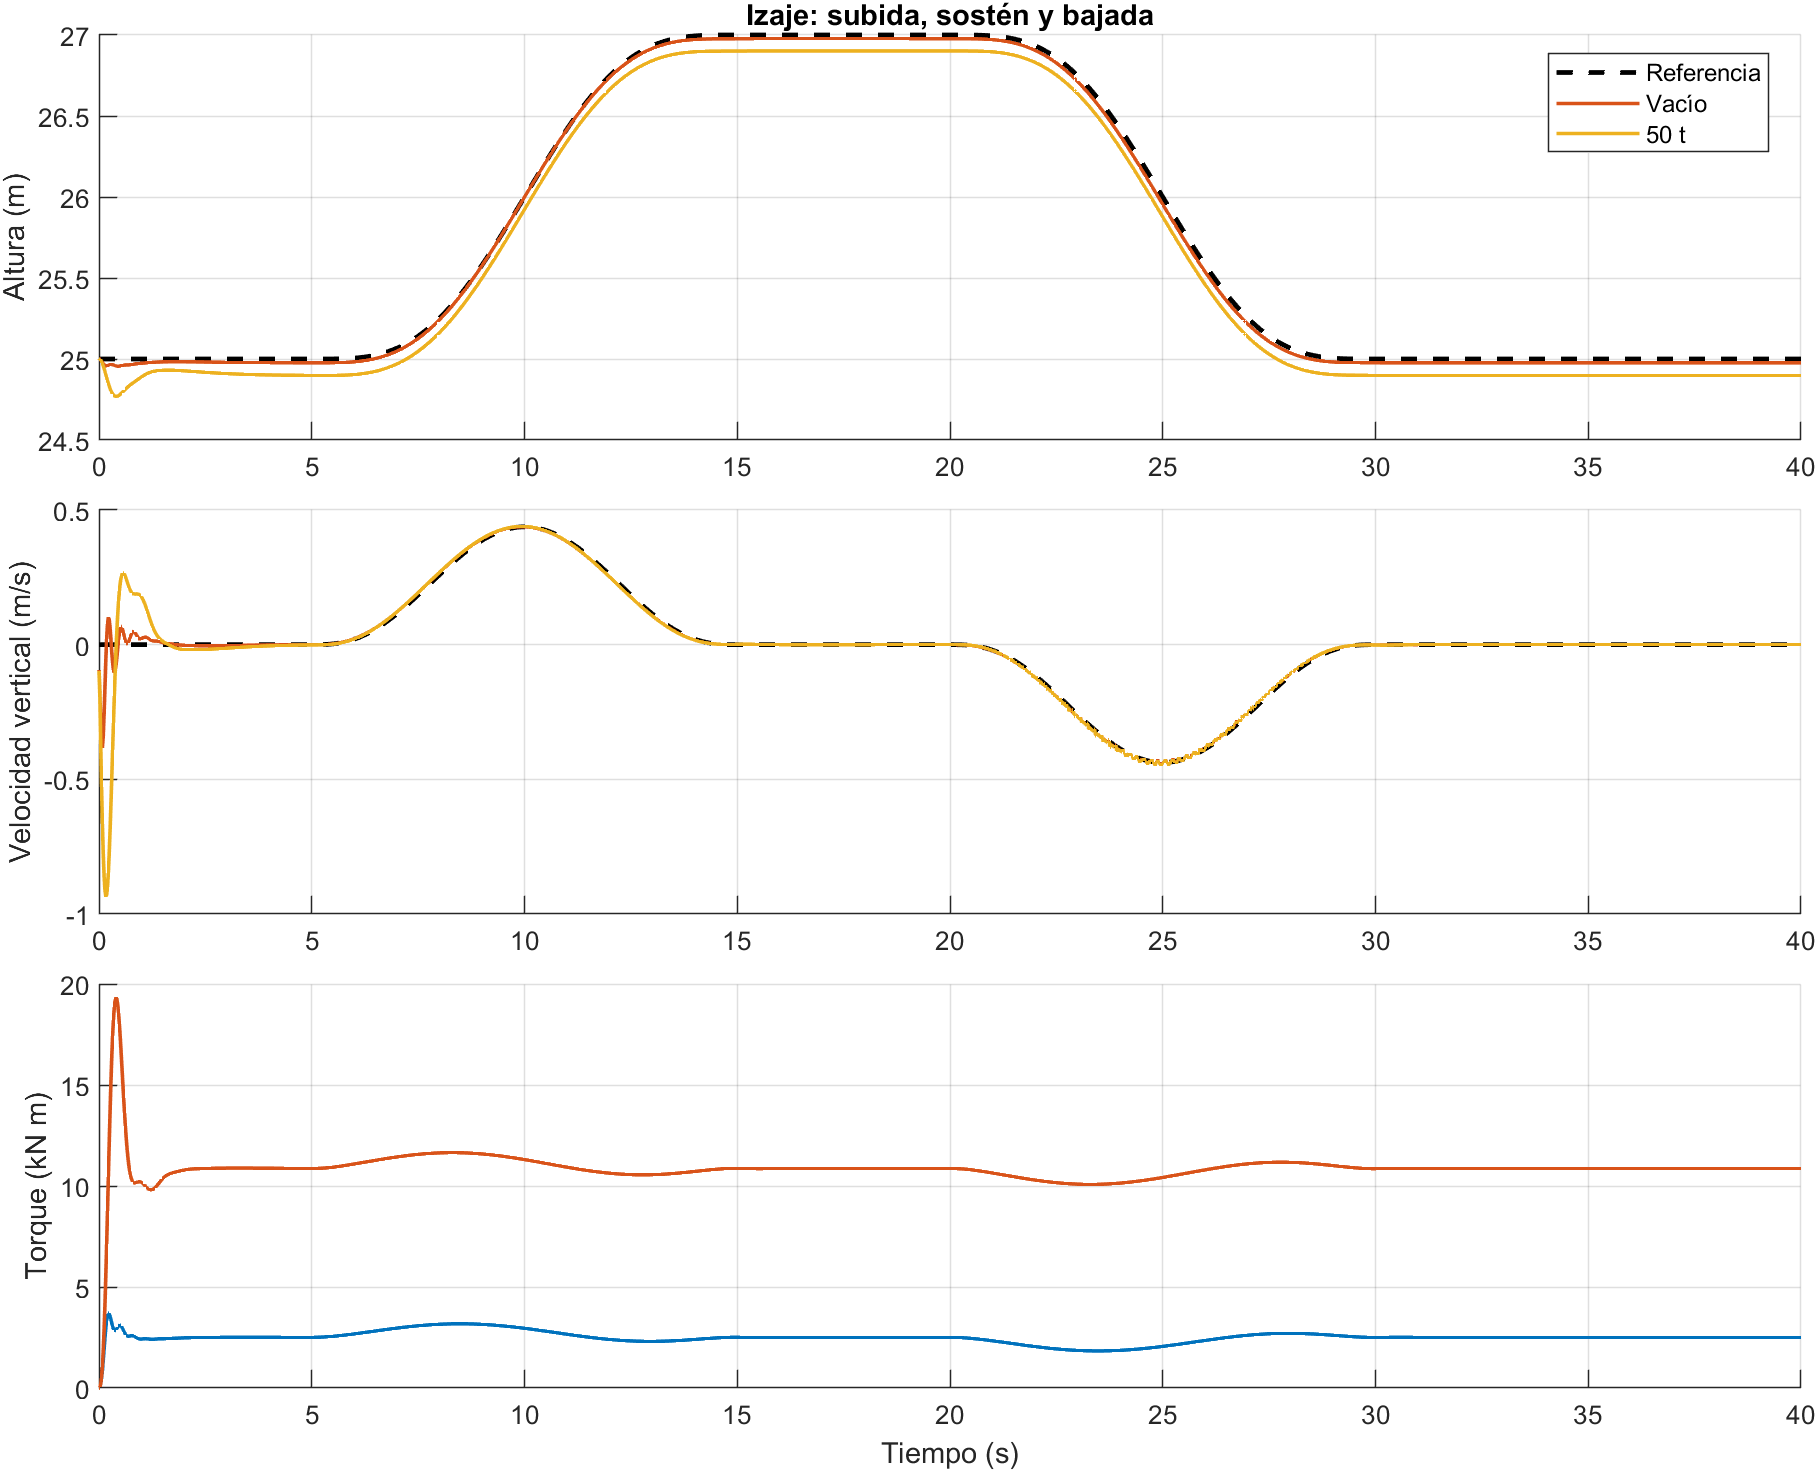
\includegraphics[width=\linewidth,height=5.35cm,keepaspectratio]{imagenes/r_039.png}
\column{.39\textwidth}
{\fontsize{8.5}{10.5}\selectfont\renewcommand{\arraystretch}{1.25}\setlength{\tabcolsep}{3pt}
\begin{tabular}{@{}lrr@{}}\toprule
Perfil / carga & RMS $e_h$ & $|T|_{\max}$\\
& [m] & [kN m]\\\midrule
Subida--bajada, 50 t & 0,1004 & 11,65\\
Subida--bajada, vacío & 0,0258 & 3,18\\
Bajada 8 m, 50 t & 0,1487 & 12,84\\
Bajada 8 m, vacío & 0,0689 & 3,81\\\bottomrule
\end{tabular}}
\end{columns}
\figcaption{Gráfica: subida, sostén y bajada. Tabla: resumen de ambos perfiles; bajada de 8 m en respaldo.}
\note{Identificar referencia y respuesta. La tabla cuantifica los dos ensayos, la gráfica muestra el primero. No generalizar los resultados a impactos de contacto ni a maniobras rápidas.}
\end{frame}
\begin{frame}[t,label=slide26]{Prueba aislada anti-sway: perturbación inicial de 7°}
\begin{center}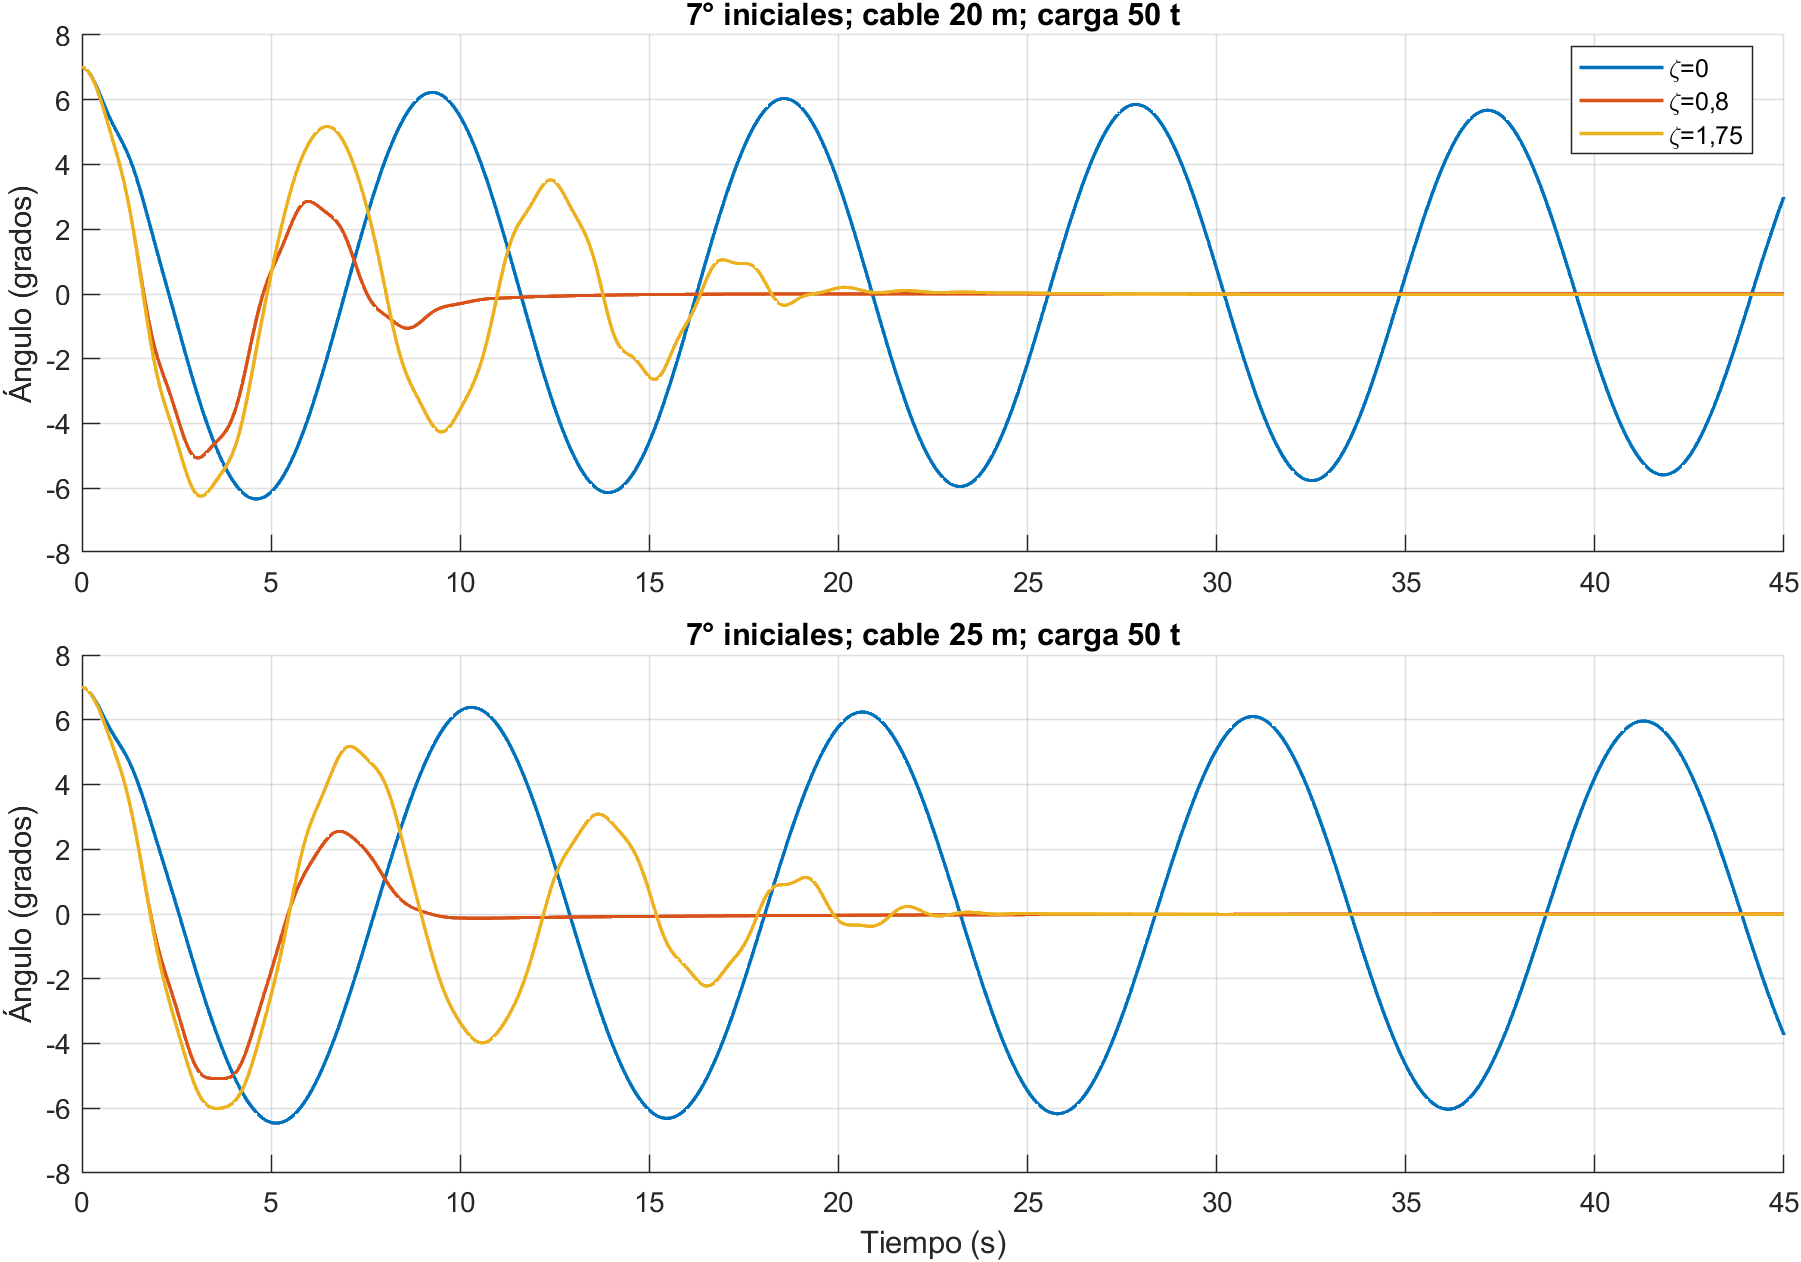
\includegraphics[width=.98\linewidth,height=5.55cm,keepaspectratio]{imagenes/r_041.png}\end{center}\vspace{-1mm}\figcaption{50 t; dos longitudes de cable; asignaciones $\zeta_{sw}=0$, $0,8$ y $1,75$.}
\note{Mostrar que aumentar zeta no mejora siempre el tiempo de estabilización. Para esta perturbación, 0,8 ofrece una respuesta más favorable que 1,75.}
\end{frame}
\begin{frame}[t,label=slide27]{Prueba del carro: traslado de 13 m en 24 s}
\relax\setlength{\parskip}{0pt}
\begin{columns}[c,onlytextwidth]
\column{.60\textwidth}
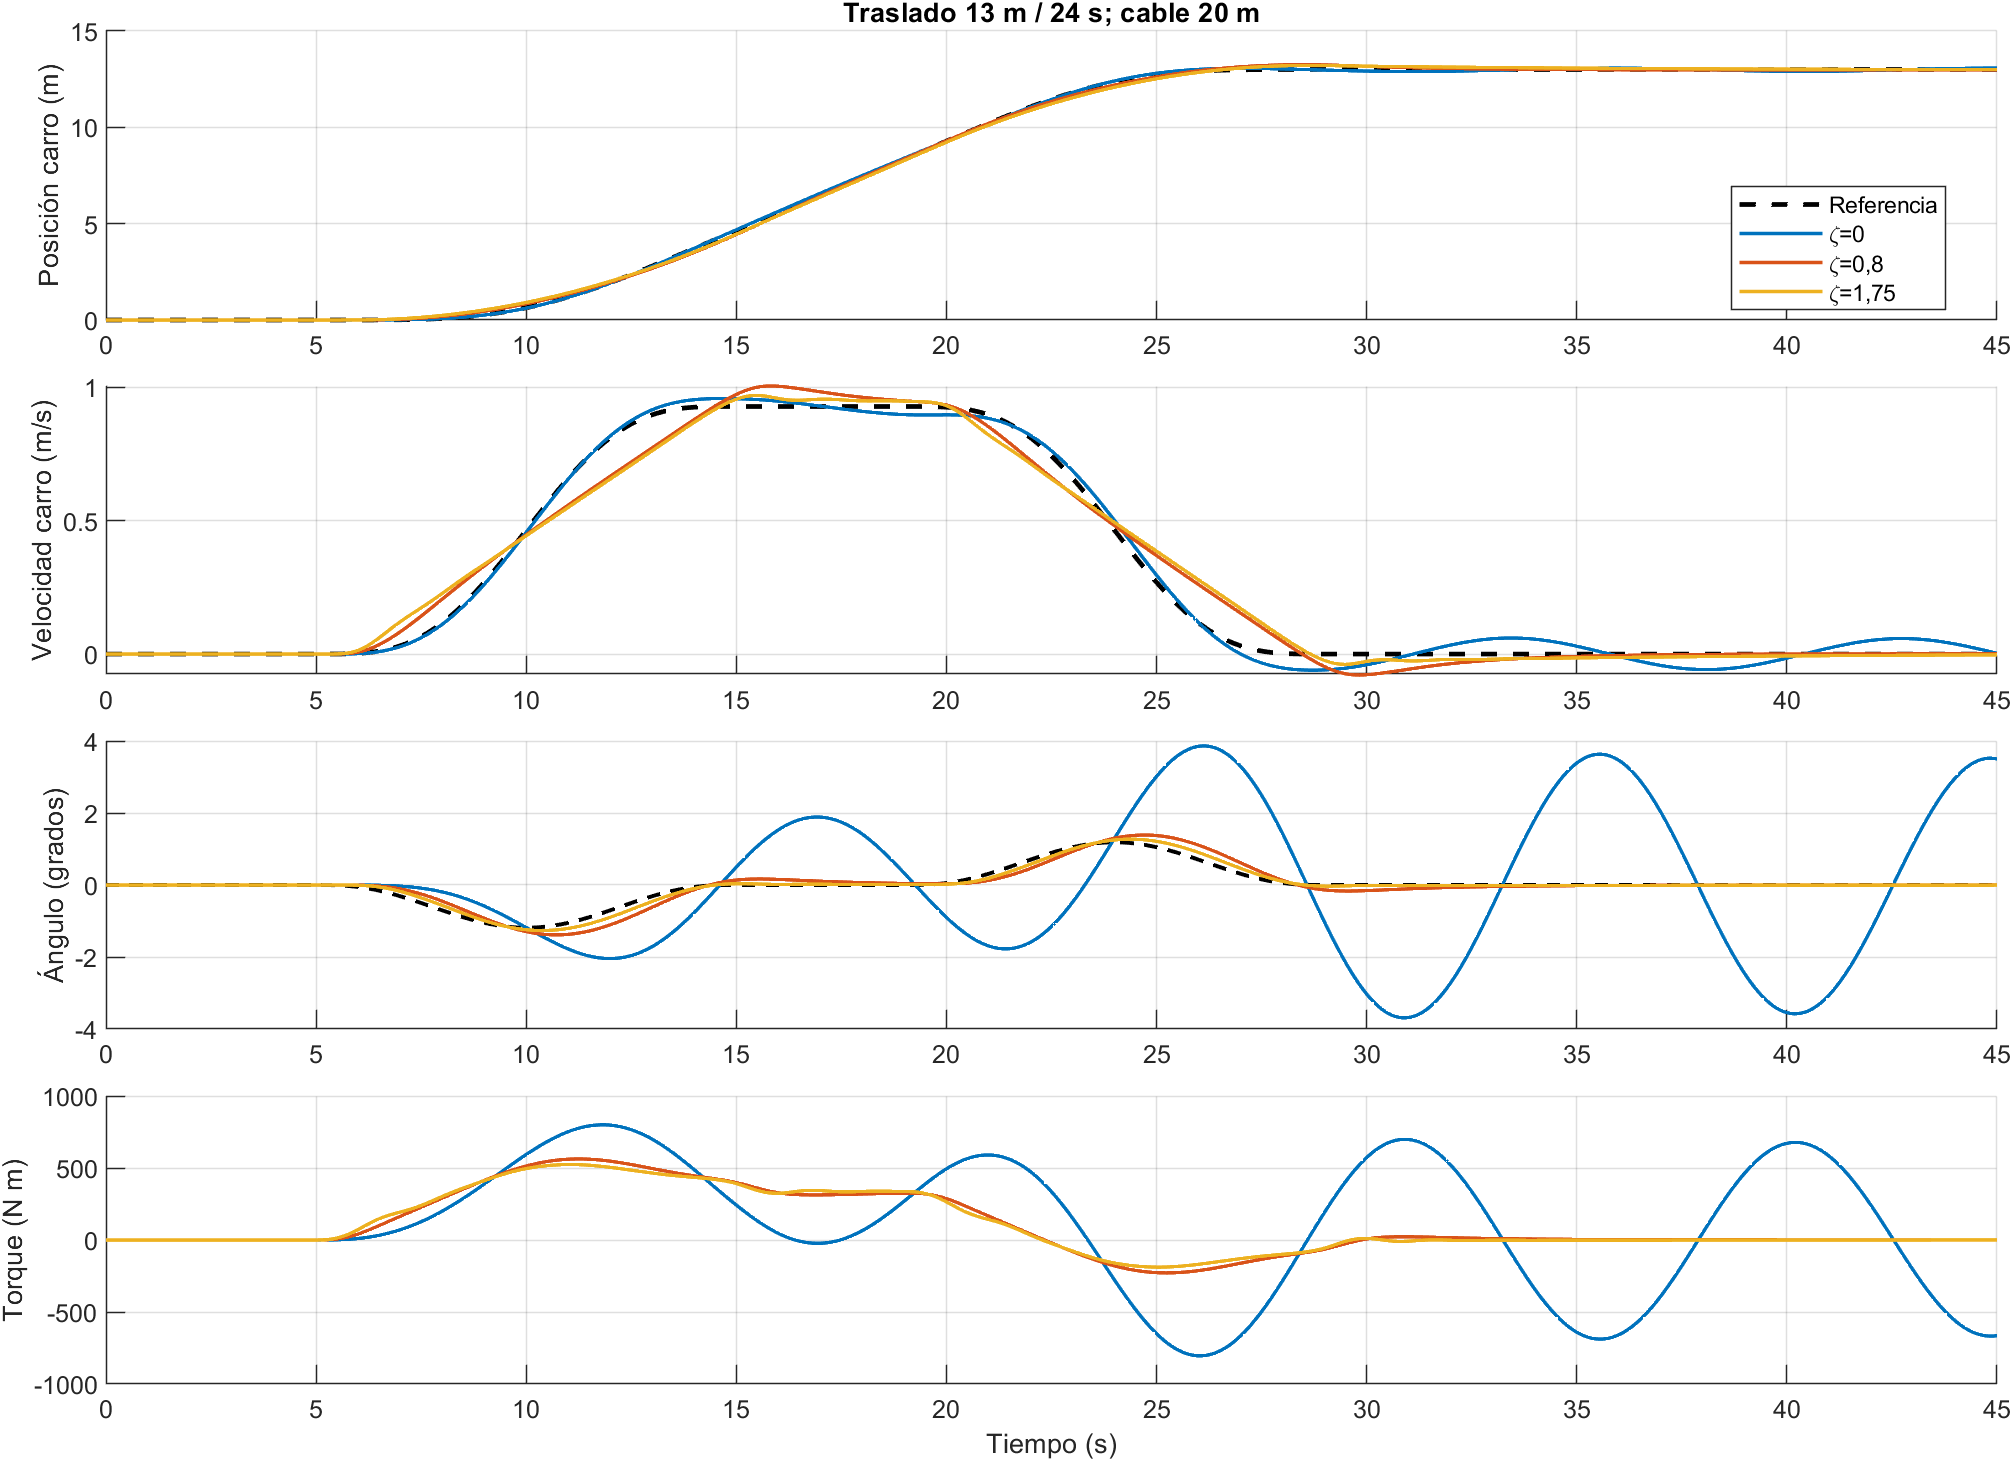
\includegraphics[width=\linewidth,height=5.35cm,keepaspectratio]{imagenes/r_042.png}
\column{.38\textwidth}
{\fontsize{8.5}{10.5}\selectfont\renewcommand{\arraystretch}{1.3}\setlength{\tabcolsep}{3pt}
\begin{tabular}{@{}lrrr@{}}\toprule
$\zeta_{sw}$ & RMS $e_x$ & RMS $\theta$ & $|T|_{\max}$\\
& [m] & [$^\circ$] & [Nm]\\\midrule
0 & 0,0424 & 1,4536 & 804,3\\
0,8 & 0,1320 & 0,2100 & 562,8\\
1,75 & 0,1668 & 0,1051 & 524,2\\\bottomrule
\end{tabular}}\par
\vspace{4mm}\figcaption{Menos balanceo requiere una corrección adicional del movimiento horizontal.}
\end{columns}
\figcaption{Traslado de 13 m en 24 s; cable de 20 m y contenedor de 50 t.}
\note{El anti-sway reduce el ángulo a cambio de un seguimiento de posición menos rígido. La comparación corresponde al traslado normal. Relacionar el compromiso con las condiciones de llegada del supervisor.}
\end{frame}
\begin{frame}[t,label=slide29]{Prueba aislada del carro: traslado rápido de 13 m}
\begin{center}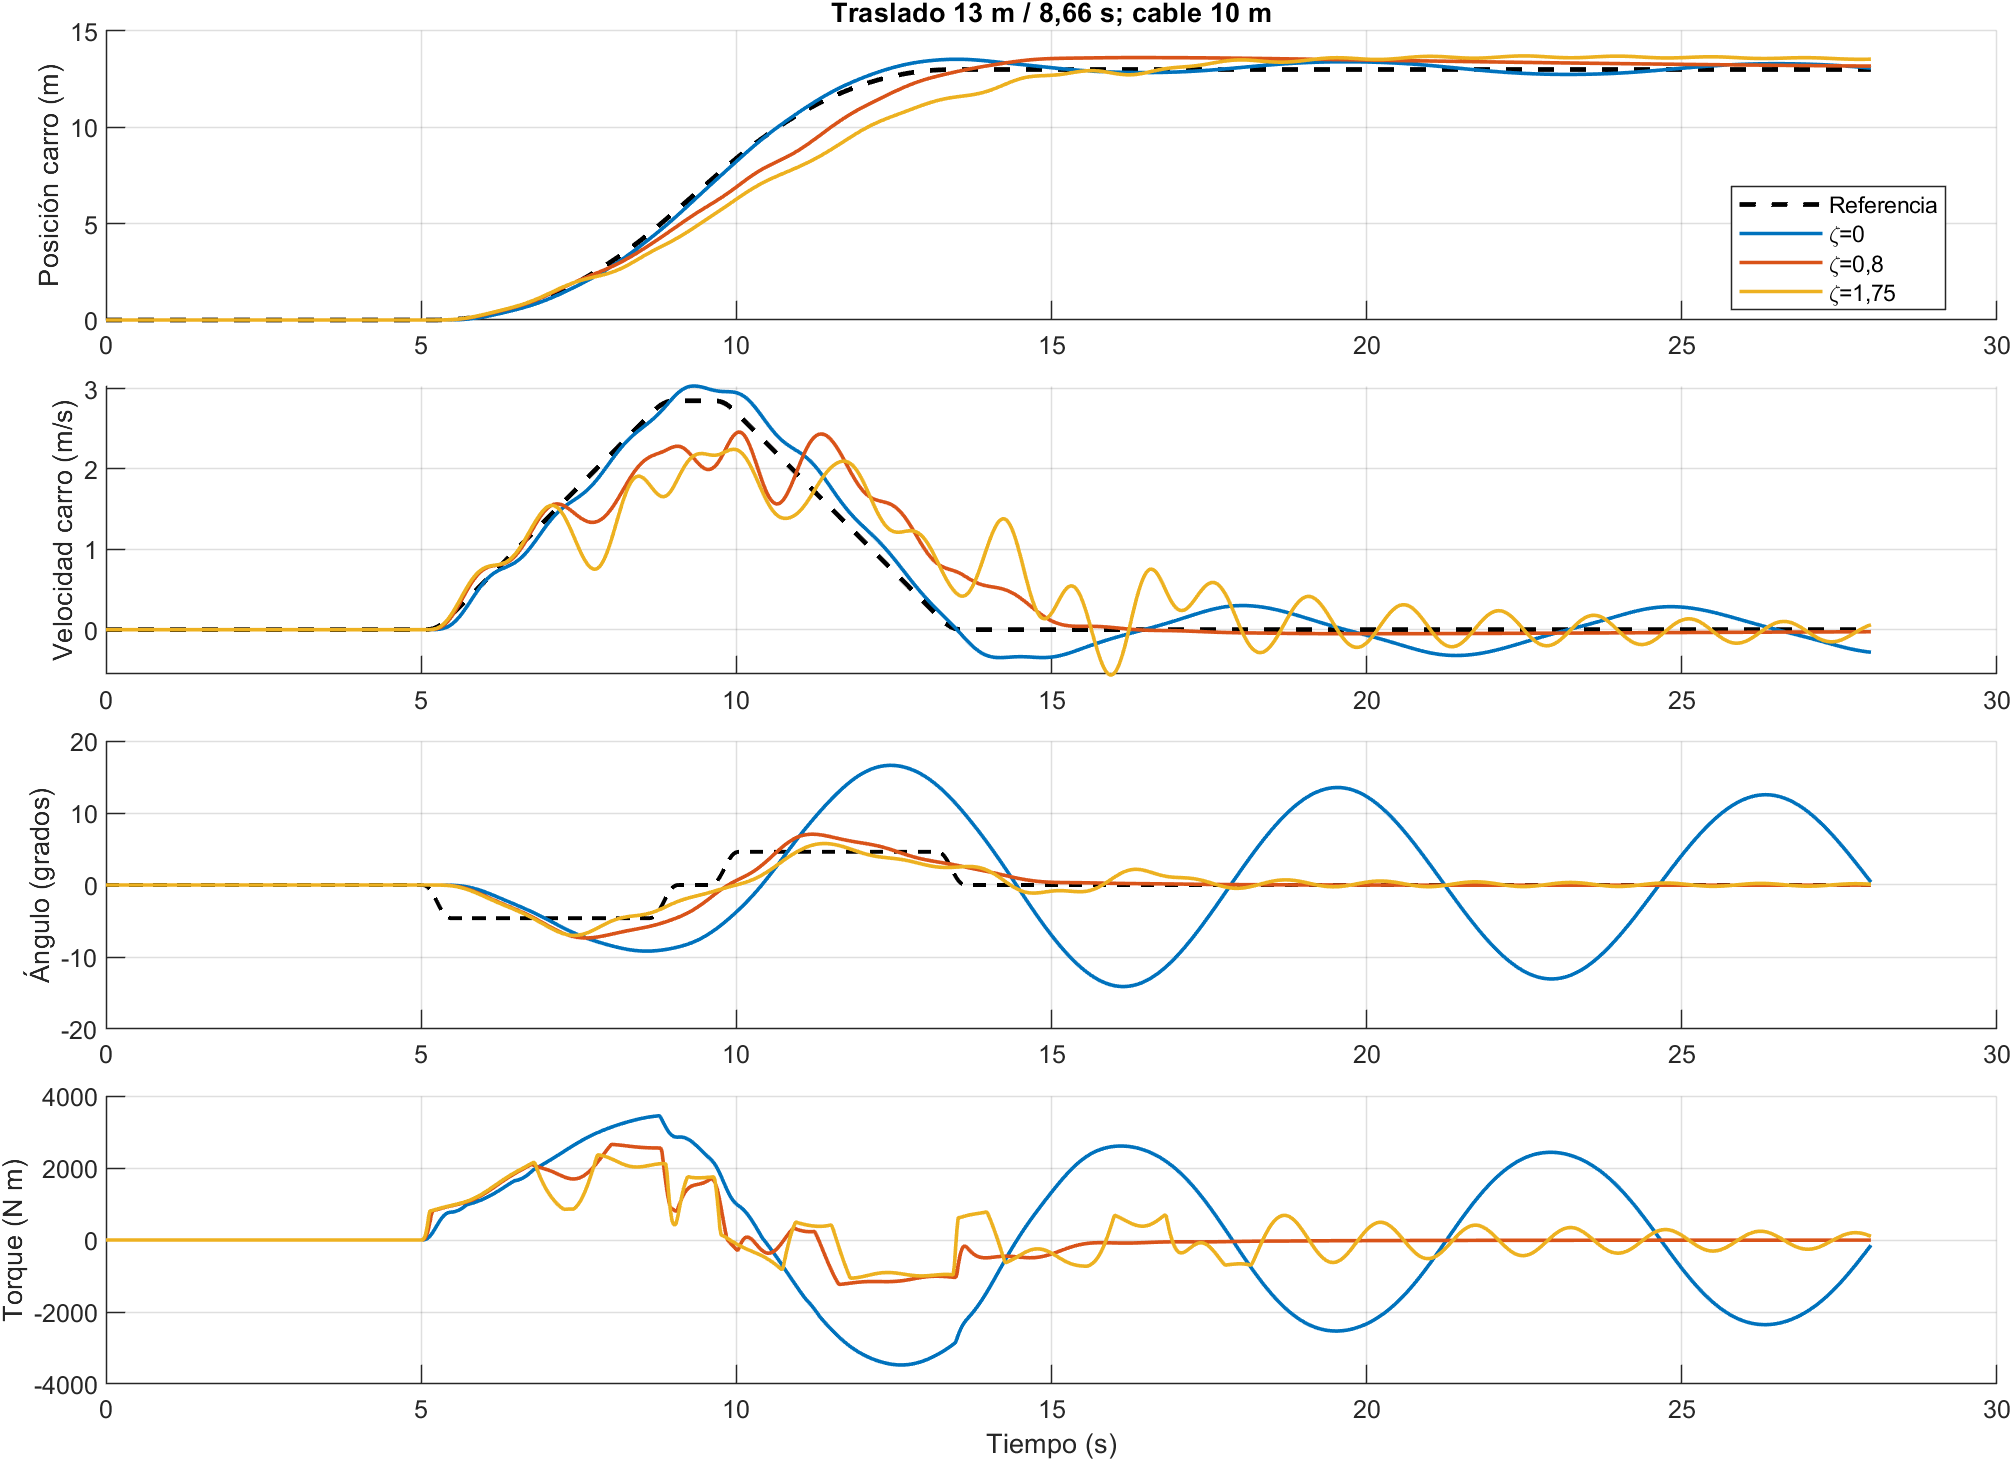
\includegraphics[width=.98\linewidth,height=5.55cm,keepaspectratio]{imagenes/r_043.png}\end{center}\vspace{-1mm}\figcaption{13 m en 8,66 s; cable de 10 m; 50 t; $v_{max}=2,85$ m/s y $a_{max}=0,792$ m/s$^2$.}
\note{La actuación del límite es prolongada y el error aumenta. Con zeta=1,75 el RMS angular baja de 6,647 a 2,037 grados, pero el error horizontal máximo llega a 2,78 m.}
\end{frame}
\section{Integración y diagnóstico del transitorio manual}
\begin{frame}[plain,label=seccion4]
\setbeamertemplate{frametitle}{}
\vfill
{\fontsize{25}{29}\selectfont\bfseries Integración y ajustes del control\par}
\vspace{4mm}\textcolor{accent}{\rule{.75\linewidth}{1pt}}\par\vspace{3mm}
{\large Referencias suaves, saturaciones y respuesta de la planta flexible.\par}\vfill
\note{Ubicar este bloque en el recorrido y anunciar su objetivo.}
\end{frame}
\begin{frame}[t,label=slide31]{Prueba de integración original: retirada del joystick}
\relax
\figurefooter{Joystick retirado a 145,800 s; pico físico a 146,744 s.}
\vspace{-2mm}\makebox[\linewidth][c]{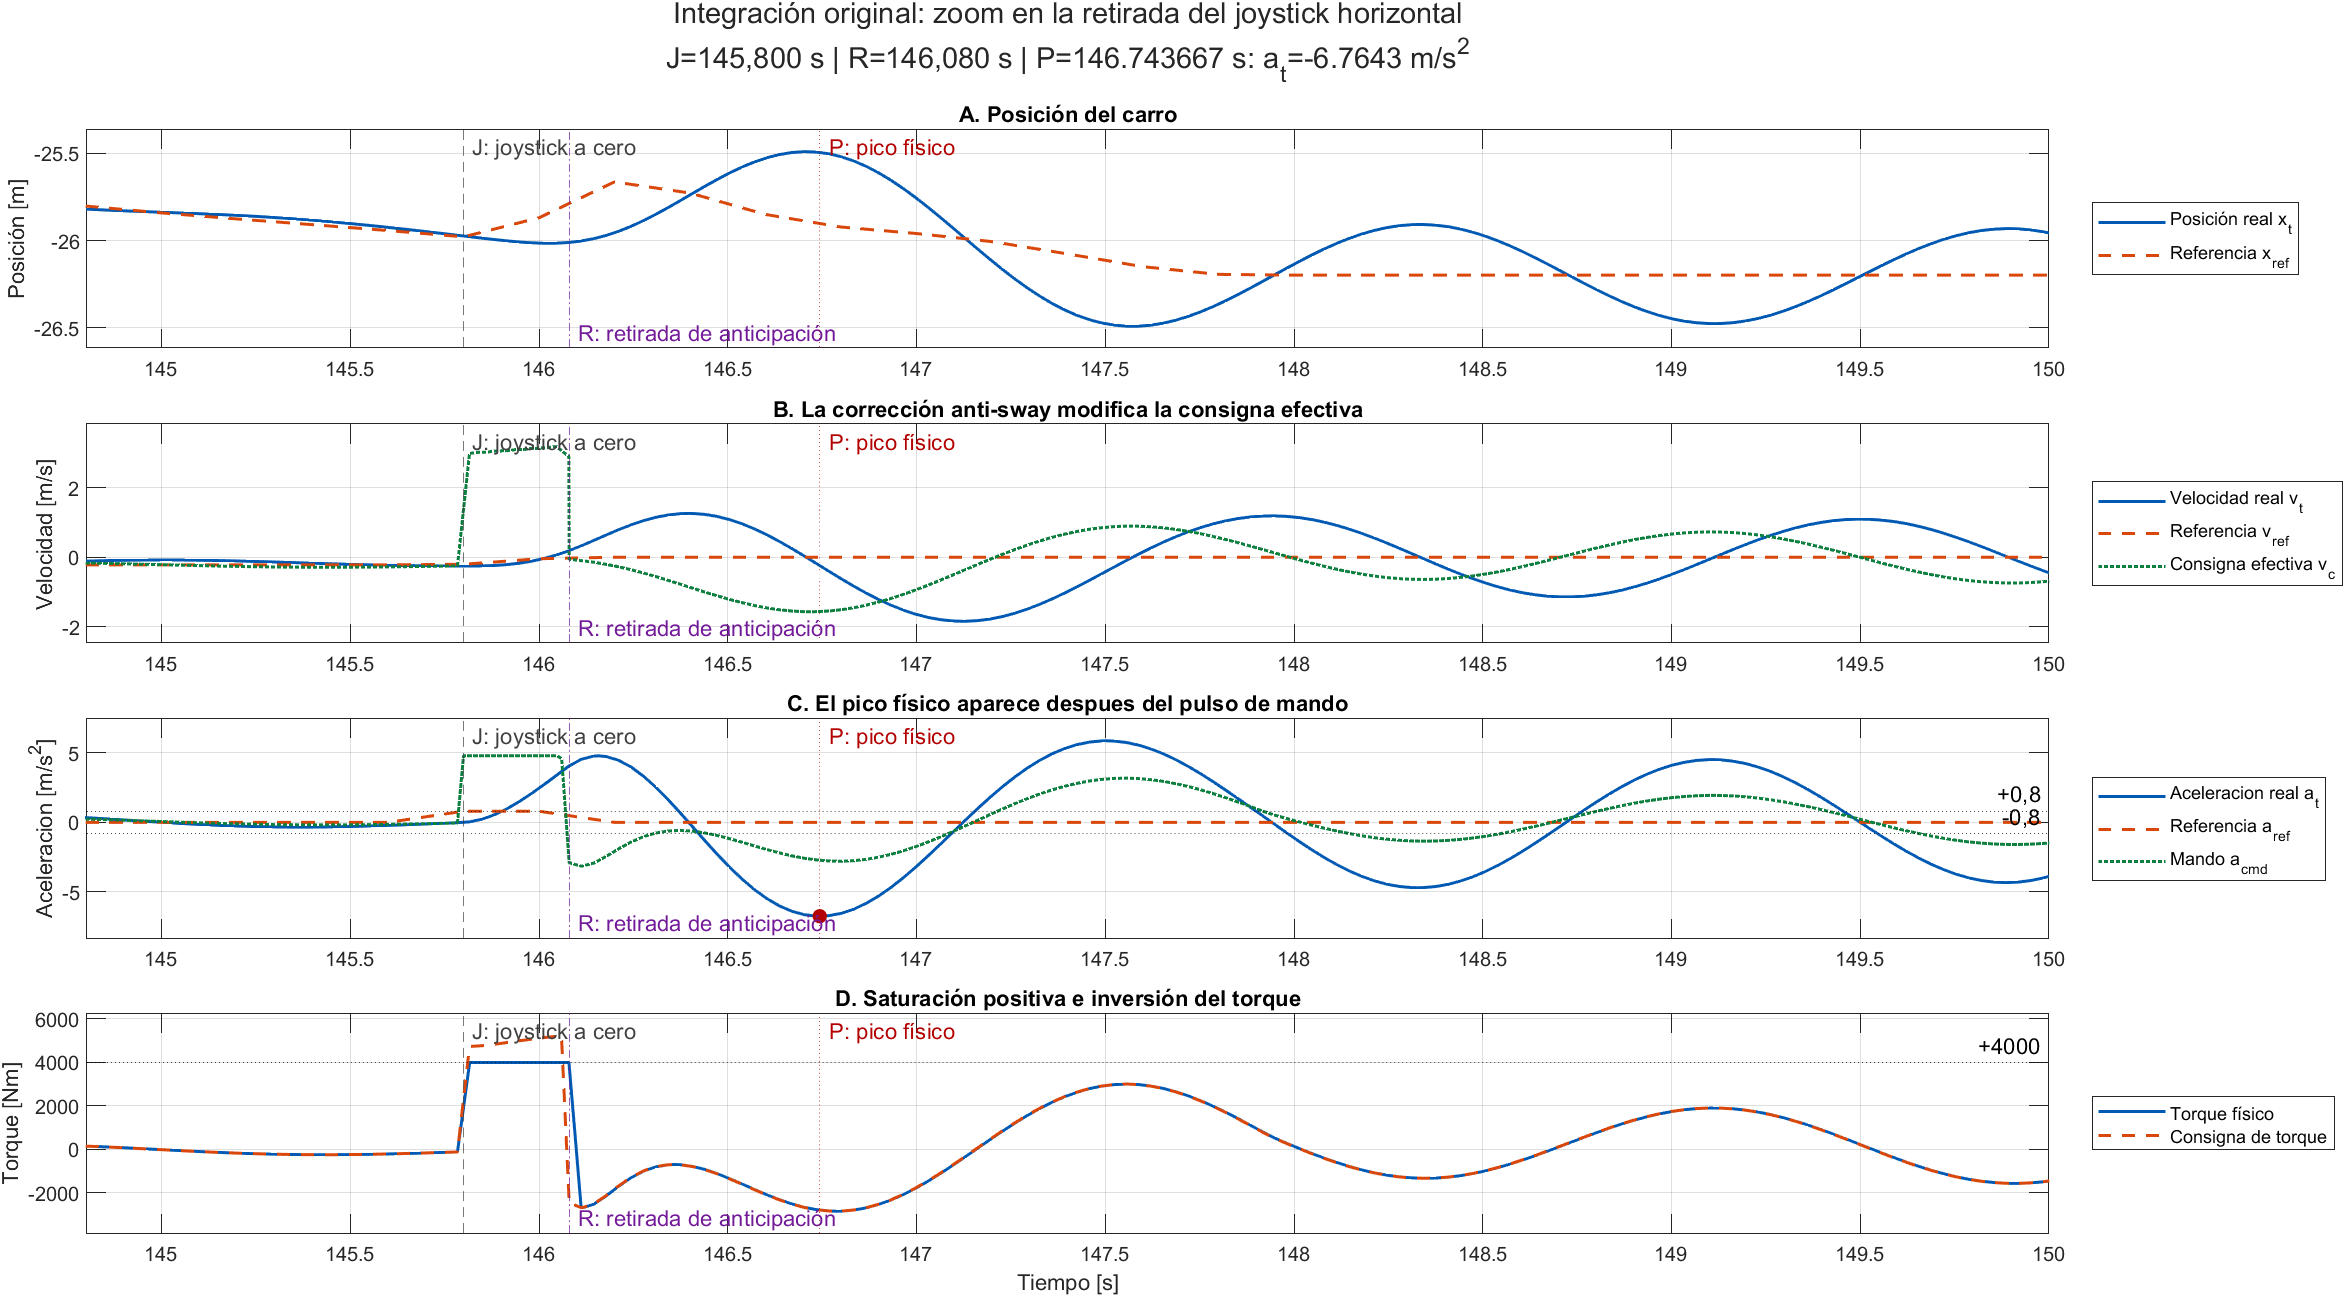
\includegraphics[width=15.0cm,height=6.05cm,keepaspectratio,trim=0.00bp 0.00bp 0.00bp 0.00bp,clip]{imagenes/r_047.png}}\par\note{Seguir la secuencia de velocidad, anticipación, mando de aceleración y torque. No identificar la curva del mando con el carro real.}
\end{frame}
\begin{frame}[t,label=slide32]{Modo flexible del carro y suavidad de las referencias}
\[
\delta=x_{td}-x_t,\quad U_e=\tfrac12K_{tw}\delta^2,\quad
\ddot\delta+K_{tw}\left(\frac1{M_d}+\frac1{M_t}\right)\delta\simeq0
\]
\[
\omega_f\simeq5{,}66\ \mathrm{rad/s},\qquad f_f\simeq0{,}90\ \mathrm{Hz}
\]
\begin{itemize}
\item La transmisión almacena energía. Limitar $a_{cmd}$ no limita directamente la aceleración física del carro.
\item El modelo reducido elimina este movimiento relativo entre dos masas.
\end{itemize}
\small\textcolor{accent}{\textbf{Durante el desarrollo:} los generadores iniciales, menos suaves y con cambios instantáneos de jerk, excitaban este modo. Se revisaron las transiciones y la anticipación anti-sway.}
\note{La observación del desarrollo fue solicitada por los autores. La frecuencia es una estimación de dos masas sin amortiguamiento, no un polo identificado. Jerk instantáneo aquí significa salto de jerk en una transición. La excitación también depende de la corrección regulatoria y del torque.}
\end{frame}
\begin{frame}[t,label=slide33]{Anti-windup: aceleración y torque}
\[
a_c=\operatorname{sat}_{0{,}8}(a_u),\qquad \Delta a_a=a_c-a_u
\]
\[
\Delta a_T=\frac{i_t}{r_{td}M_{EQt}}(T_{lim}-T_{in})
\]
\[
\dot I=e_v+\frac{\Delta a_a+\Delta a_T}{K_{iv}T_{aw}},\quad T_{aw}=1\ \mathrm{s}
\]
\begin{itemize}
\item El recorte de torque se mide antes de la dinámica del motor.
\item Ambos límites corrigen el mismo estado integral.
\item La suma completa de aceleraciones se limita a ±0,80 m/s².
\end{itemize}
\note{Evitar medir saturación con torque físico menos torque limitado: eso incorpora el retardo del motor. La realización discreta exacta queda en la sección MC.}
\end{frame}
\begin{frame}[t,label=slide34]{Anticipación anti-sway limitada}
\[
v_{sw}=\operatorname{sat}_{3{,}2}\!\left[\alpha(t)\left(k_{sw}\theta_l+v_{ff,lim}\right)\right]
\]
\[
v_{ff}=-k_{sw}\theta_{ref},\qquad k_{sw}=2\zeta_{sw}\sqrt{g/l_h}\,l_h
\]
\begin{itemize}
\item Se limita la variación del término anticipativo: 0,25 m/s².
\item Se conserva la realimentación angular directa.
\item Rampa de habilitación de 2 s.
\item Se conserva el PI, el anti-windup y la compensación mecánica.
\end{itemize}
\note{Aclarar que el límite de 0,25 tiene unidades de derivada de una corrección de velocidad. No es el límite de aceleración física del carro; la estructura de frenado permanece.}
\end{frame}
\begin{frame}[t,label=slide35]{Prueba de anticipación limitada: referencias y mando}
\relax\setlength{\parskip}{0pt}
\figurefooter{Ley simple y FF limitado, ambas con anti-windup y condiciones comparables.}
\vspace{-3mm}\makebox[\linewidth][c]{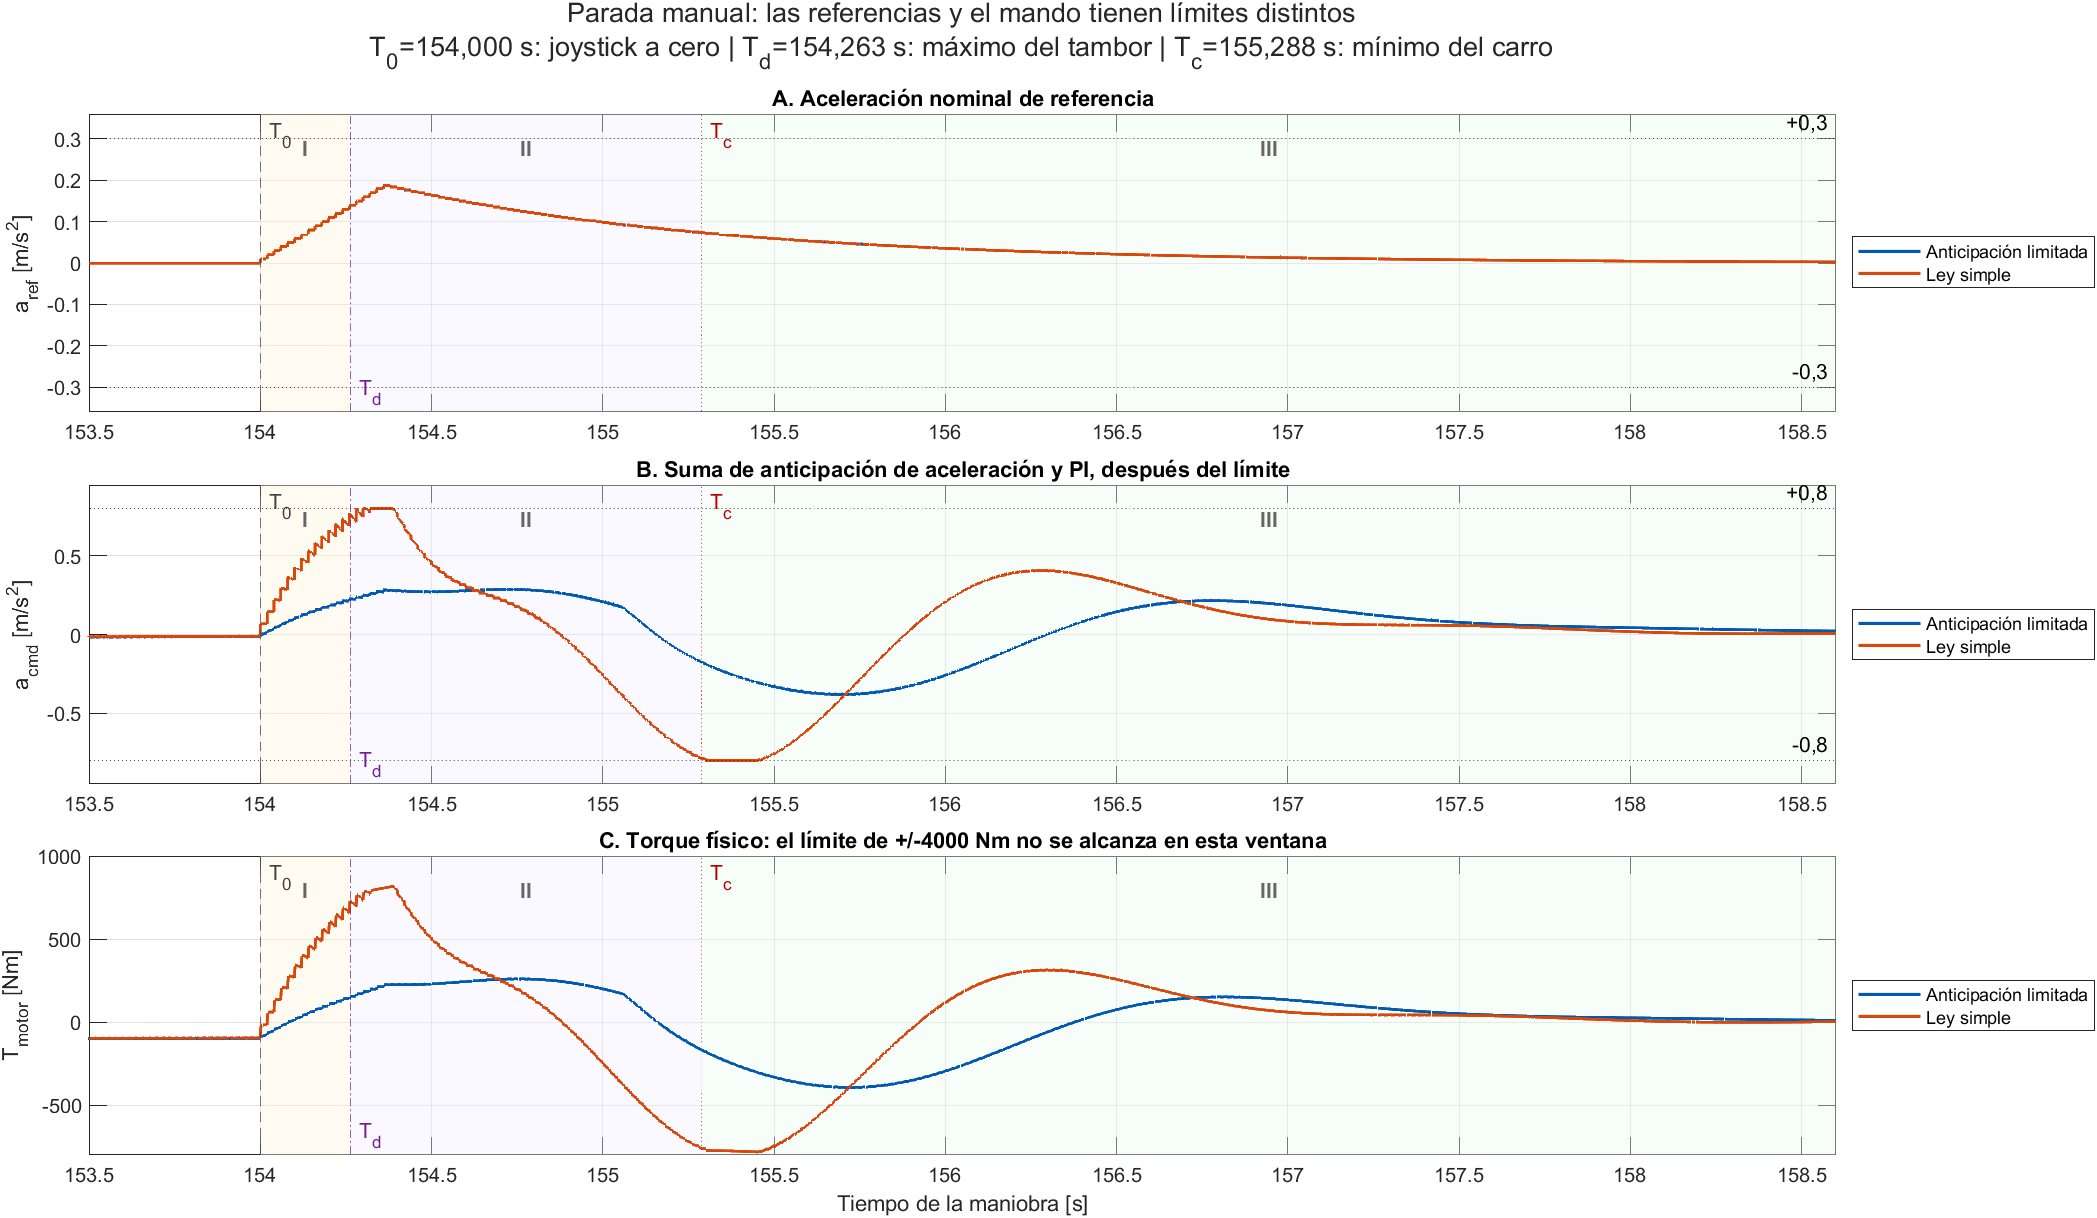
\includegraphics[width=15.0cm,height=6.55cm,keepaspectratio,trim=0.00bp 0.00bp 0.00bp 0.00bp,clip]{imagenes/r_048.png}}\par\note{El mando regulatorio permanece dentro del límite en ambas variantes. La diferencia aparece al observar la aceleración física y el esfuerzo mecánico.}
\end{frame}
\begin{frame}[t,label=slide36]{Prueba de anticipación limitada: energía elástica}
\relax\setlength{\parskip}{0pt}
\figurefooter{La anticipación limitada reduce la excitación de la transmisión durante la parada.}
\vspace{-3mm}\makebox[\linewidth][c]{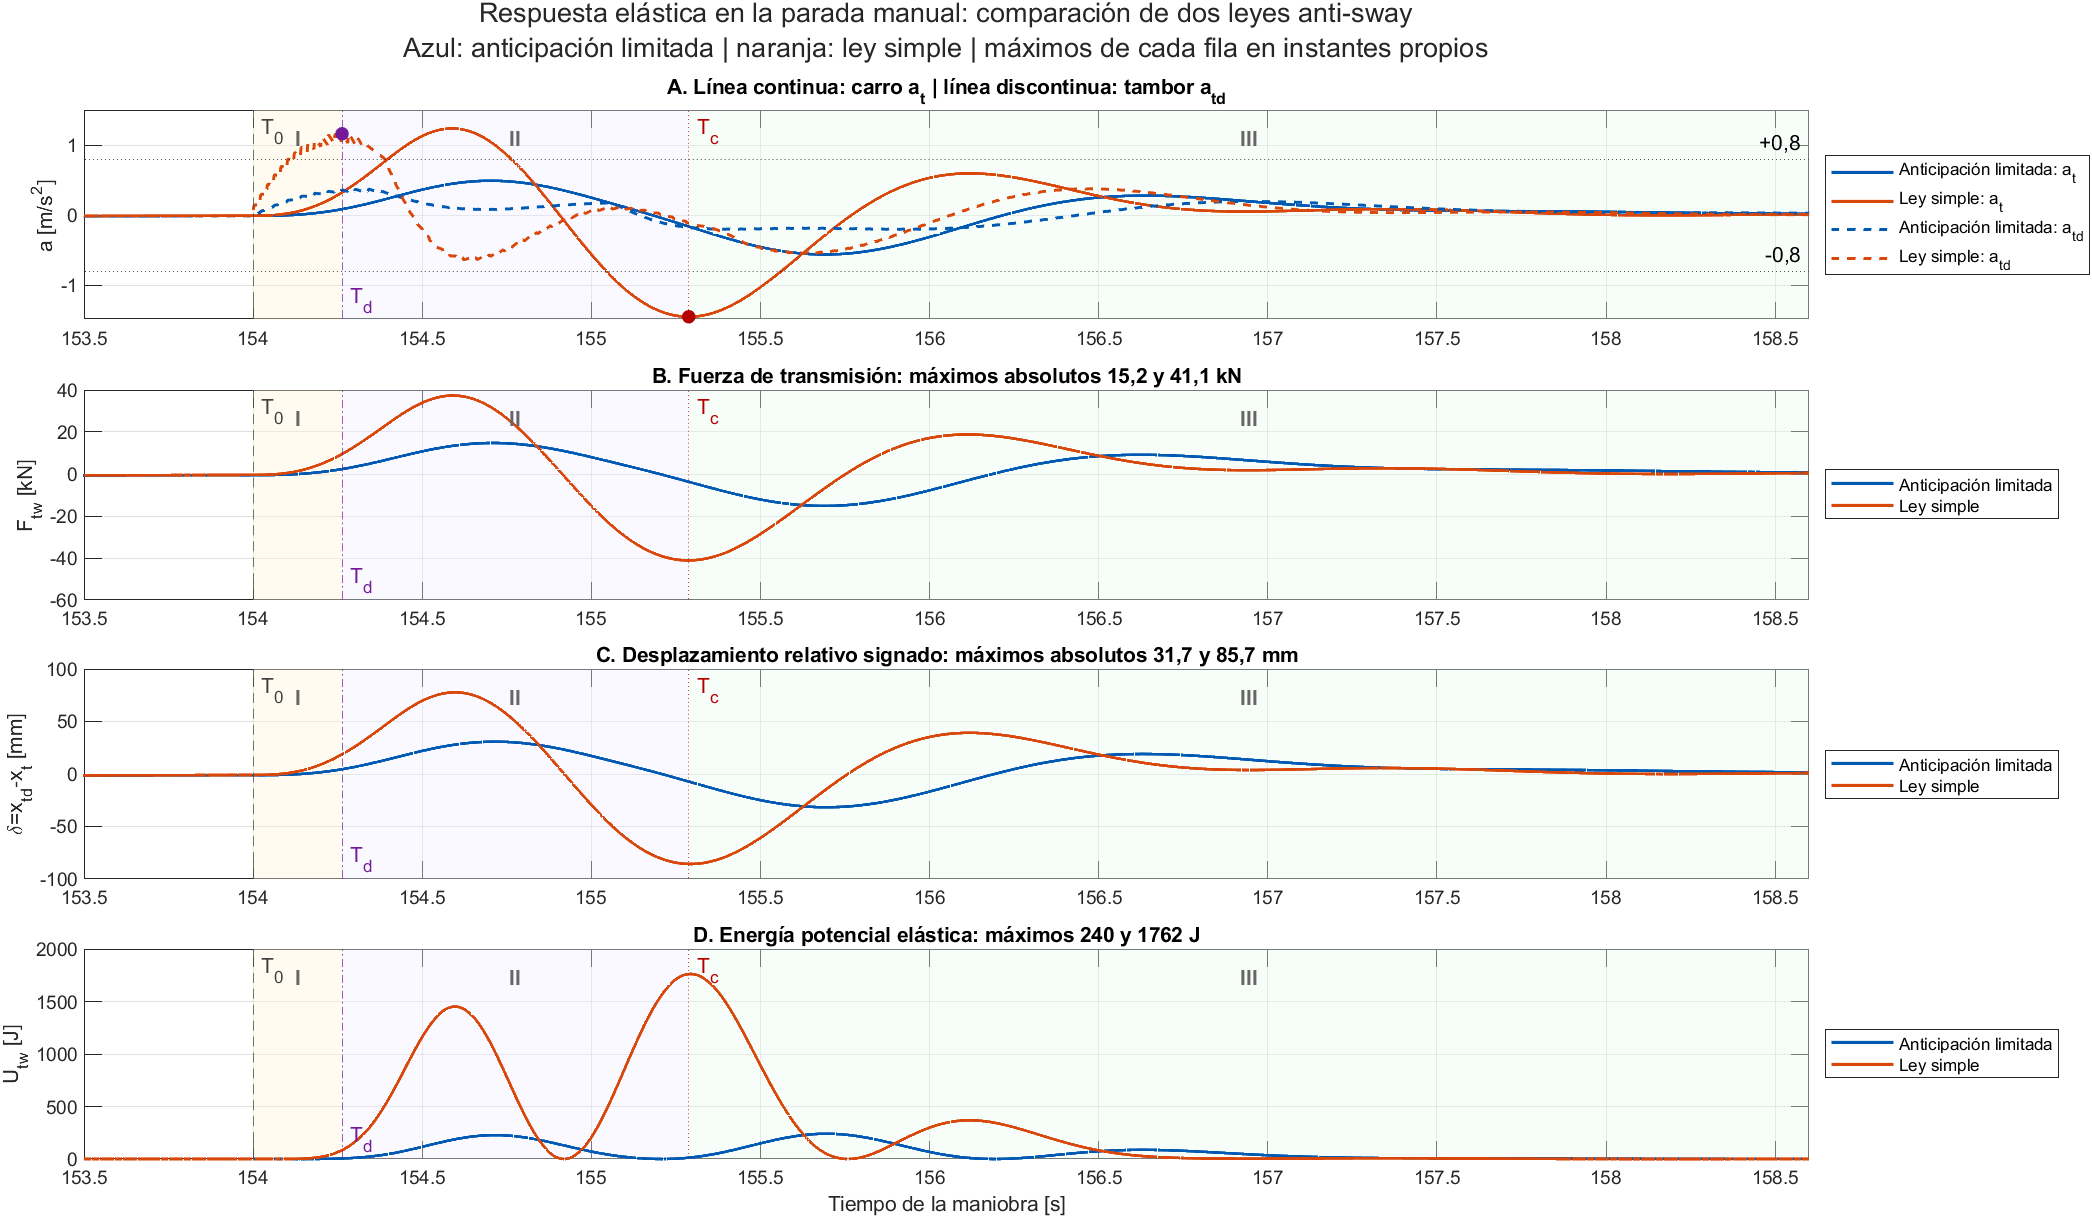
\includegraphics[width=15.0cm,height=6.55cm,keepaspectratio,trim=0.00bp 0.00bp 0.00bp 0.00bp,clip]{imagenes/r_049.png}}\par\note{Destacar la diferencia entre aceleración del tambor y del carro. Recorrer fuerza y energía como evidencia de la causa física.}
\end{frame}
\begin{frame}[t,label=slide37]{Prueba de anticipación limitada: resultados}
\begin{center}
{\small\renewcommand{\arraystretch}{1.0}
\begin{tabular}{lrr}\toprule
Magnitud & Ley simple & FF limitado\\\midrule
Aceleración física máxima [m/s²] & 1,4535 & 0,6274\\
Tiempo fuera de ±0,80 m/s² [s] & 0,8836 & 0\\
Fuerza máxima [kN] & 41,142 & 15,198\\
Energía elástica máxima [J] & 1 762,084 & 240,485\\
Duración de la maniobra [s] & 381,20 & 381,40\\
\bottomrule\end{tabular}}\end{center}
\vspace{2mm}\textcolor{accent}{\textbf{Reducción de energía elástica máxima: 86,4 \%.}}
\note{La mejora principal es de excitación y esfuerzo, con incidencia pequeña sobre la duración. No afirmar que la estabilización resulta más rápida: en esta ventana el tiempo medido no mejora.}
\end{frame}
\section{Supervisor y planificación coordinada}
\begin{frame}[plain,label=seccion5]
\setbeamertemplate{frametitle}{}
\vfill
{\fontsize{25}{29}\selectfont\bfseries Supervisor y planificación del movimiento\par}
\vspace{4mm}\textcolor{accent}{\rule{.75\linewidth}{1pt}}\par\vspace{3mm}
{\large Estados, secuencias y referencias coordinadas para ambos ejes.\par}\vfill
\note{Ubicar este bloque en el recorrido y anunciar su objetivo.}
\end{frame}
\begin{frame}[t,label=cmp1]{Organización del supervisor · Stateflow}
\begin{center}\diagramfit{\begin{tikzpicture}
\node[sfstate,dashed,text width=3.8cm](r0)at(0.0,0.0){1. INTERLOCKS\\{\scriptsize Prepara guardas}};
\node[sfstate,dashed,text width=3.8cm](r1)at(4.8,0.0){2. CARGA Y TWISTLOCKS\\{\scriptsize Gestiona toma y masa}};
\node[sfstate,dashed,text width=3.8cm](r2)at(9.6,0.0){3. OPERACIÓN\\{\scriptsize Selecciona maniobra}};
\node[sfstate,dashed,text width=3.8cm](r3)at(0.0,-2.0){4. REFERENCIAS CARRO\\{\scriptsize Actualiza referencias}};
\node[sfstate,dashed,text width=3.8cm](r4)at(4.8,-2.0){5. FRENOS\\{\scriptsize Coordina apertura}};
\node[sfstate,dashed,text width=3.8cm](r5)at(9.6,-2.0){6. DIAGNÓSTICO\\{\scriptsize Publica códigos}};
\end{tikzpicture}}\end{center}\vfill
{\small Seis regiones paralelas se ejecutan en orden cada 20 ms.\par}\vspace{1.5mm}{\fontsize{9.5}{11}\selectfont\textcolor{muted}{Las referencias comunes se actualizan después de OPERACIÓN y antes de FRENOS.}\par}

\note{Seis regiones paralelas se ejecutan en orden cada 20 ms. Las referencias comunes se actualizan después de OPERACIÓN y antes de FRENOS.}
\end{frame}

\begin{frame}[t,label=cmp2]{Organización del supervisor · CODESYS SFC}
\begin{center}\diagramfit{\begin{tikzpicture}
\node[sfcstep,double,double distance=1pt] (init) at (5.5,1.75){INICIAL};
\draw[wire](init.south)--(5.5,.82);
\draw[wire,line width=1pt](5.3,1.05)--(5.7,1.05);
\node[guard,anchor=west]at(5.85,1.05){Sin parada ni pérdida de permiso};
\draw[wire,line width=1pt](-1.2,0.82)--(12.2,0.82);
\draw[wire,line width=1pt](-1.2,0.75)--(12.2,0.75);
\draw[wire,line width=1pt](-1.2,-0.75)--(12.2,-0.75);
\draw[wire,line width=1pt](-1.2,-0.82)--(12.2,-0.82);
\node[sfcstep,text width=2.2cm](r0)at(0.0,0){REGIÓN OPERACIÓN};
\draw[wire](0.0,.75)--(r0.north);
\draw[wire](r0.south)--(0.0,-.75);
\node[sfcstep,text width=2.2cm](r1)at(2.75,0){CARGA};
\draw[wire](2.75,.75)--(r1.north);
\draw[wire](r1.south)--(2.75,-.75);
\node[sfcstep,text width=2.2cm](r2)at(5.5,0){FRENO\\IZAJE};
\draw[wire](5.5,.75)--(r2.north);
\draw[wire](r2.south)--(5.5,-.75);
\node[sfcstep,text width=2.2cm](r3)at(8.25,0){FRENO\\CARRO};
\draw[wire](8.25,.75)--(r3.north);
\draw[wire](r3.south)--(8.25,-.75);
\node[sfcstep,text width=2.2cm](r4)at(11.0,0){DIAGNÓSTICO};
\draw[wire](11.0,.75)--(r4.north);
\draw[wire](r4.south)--(11.0,-.75);
\node[sfcstep](stop)at(5.5,-1.8){DETENIDO};
\draw[wire](5.5,-.82)--(stop.north);
\draw[wire,line width=1pt](5.3,-1.05)--(5.7,-1.05);
\node[guard,anchor=west]at(5.85,-1.05){Parada o pérdida de permiso};
\node[guard,anchor=north,align=center]at(5.5,-2.3){Reset y permiso global: salto a INICIAL};
\end{tikzpicture}}\end{center}\vfill
{\small Las ramas SFC agrupan responsabilidades. La tarea llama a las secuencias y a los cálculos ST.\par}\vspace{1.5mm}{\fontsize{9.5}{11}\selectfont\textcolor{muted}{El estado activo de un paso se consulta desde ST para generar referencias y órdenes.}\par}

\note{Las ramas SFC agrupan responsabilidades. La tarea llama a las secuencias y a los cálculos ST. El estado activo de un paso se consulta desde ST para generar referencias y órdenes.}
\end{frame}

\begin{frame}[t,label=cmp3]{INTERLOCKS · Stateflow}
\begin{center}\diagramfit{\begin{tikzpicture}
\node[sfstate,text width=2.5cm] (n0) at (0.0,0) {INTERLOCKS\\región activa};
\node[sfstate,text width=2.5cm] (n1) at (3.35,0) {Banderas y\\variables comunes};
\node[sfstate,text width=2.5cm] (n2) at (6.7,0) {Carga, operación,\\frenos y diagnóstico};
\fill[accent] (-1.8,0) circle (2pt);
\draw[flow] (-1.8,0)--(n0.west);
\draw[flow] (n0.east)--(n1.west);
\node[guard,text width=3.35cm,anchor=south] at (1.675,.78) {Acondicionamiento\\cada 20 ms};
\draw[flow] (n1.east)--(n2.west);
\node[guard,text width=3.35cm,anchor=south] at (5.025,1.18) {Uso en el mismo ciclo};
\end{tikzpicture}}\end{center}\vfill
{\small Acondiciona entradas y memoriza solicitudes breves del HMI.\par}\vspace{1.5mm}{\fontsize{9.5}{11}\selectfont\textcolor{muted}{Calcula estabilidad, masa, límites locales y condiciones de acceso al automático.}\par}

\note{Acondiciona entradas y memoriza solicitudes breves del HMI. Calcula estabilidad, masa, límites locales y condiciones de acceso al automático.}
\end{frame}

\begin{frame}[t,label=cmp4]{INTERLOCKS · CODESYS SFC}
\begin{center}\diagramfit{\begin{tikzpicture}
\node[sfcstep,double,double distance=1pt] (p) at (0,0) {PREPROCESO};
\node[sfcstep] (s) at (0,-1.2) {EVALUACIÓN SFC};
\node[sfcstep] (a) at (0,-2.4) {ACCIONES Y SALIDAS};
\draw[wire](p.south)--(s.north);
\draw[wire,line width=1.1pt](-.2,-.6)--(.2,-.6);
\node[guard,anchor=west,text width=4.8cm]at(1.7,-.6){Fin del preprocesamiento};
\draw[wire](s.south)--(a.north);
\draw[wire,line width=1.1pt](-.2,-1.8)--(.2,-1.8);
\node[guard,anchor=west,text width=4.8cm]at(1.7,-1.8){Fin de evaluación de los pasos};
\draw[wire](a.south)--(0,-3.0);
\draw[wire,line width=1.1pt](-.2,-2.85)--(.2,-2.85);
\draw[flow](0,-3.0)--(-2.25,-3.0)--(-2.25,.65)-|(p.north);
\node[guard,anchor=west,text width=4.8cm]at(1.7,-2.85){Siguiente ciclo de 20 ms};
\node[draw=ink,align=left,font=\fontsize{9}{10}\selectfont,text width=4.4cm,anchor=west]at(7.0,0){N: ST prepara banderas, guardas y solicitudes del HMI};
\node[draw=ink,align=left,font=\fontsize{9}{10}\selectfont,text width=4.4cm,anchor=west]at(7.0,-1.2){N: evalúa las secuencias con las banderas compartidas};
\node[draw=ink,align=left,font=\fontsize{9}{10}\selectfont,text width=4.4cm,anchor=west]at(7.0,-2.4){N: ST consulta pasos activos y aplica interbloqueos finales};
\draw[wire](p.east)--(7.0,0);\draw[wire](s.east)--(7.0,-1.2);\draw[wire](a.east)--(7.0,-2.4);
\end{tikzpicture}}\end{center}\vfill
{\small El preprocesamiento prepara las guardas antes de evaluar las secuencias SFC.\par}
\vspace{1.5mm}{\fontsize{9.5}{11}\selectfont\textcolor{muted}{Esquema funcional en notación SFC del orden de ejecución. Los cálculos y las salidas permanecen en ST.}\par}

\note{El esquema usa pasos, transiciones y acciones para explicar el orden de ejecución cíclica. El preprocesamiento prepara las entradas y guardas, después se evalúan las secuencias SFC y finalmente las acciones ST consultan los pasos activos y aplican los interbloqueos. N indica acción no almacenada asociada al paso. Los textos de las transiciones describen el fin de cada fase. Este dibujo representa funcionalmente el orden de llamadas del PLC, sin introducir un nuevo POU INTERLOCKS en SFC ni cambiar la implementación real.}
\end{frame}


\begin{frame}[t,label=cmp5]{Operación: arranque y parada · Stateflow}
\begin{center}\diagramfit{\begin{tikzpicture}
\node[sfstate](off) at(0,0){APAGADO};\node[sfstate](start)at(4.4,0){ARRANQUE};\node[sfstate](ready)at(8.8,0){LISTO};
\draw[flow](off)--node[guard,above,text width=3cm,yshift=6mm]{Start, configuración\\y permiso global}(start);
\draw[flow](start)--node[guard,above,text width=3cm,yshift=6mm]{Permisos por eje\\y 5 ticks}(ready);
\node[sfstate](stop)at(1.8,-2){PARADA NORMAL};\node[sfstate](fail)at(7,-2){RETENCIÓN FALLA};
\draw[flow](stop.west)-|node[guard,pos=.12,above,xshift=-12mm]{Ejes detenidos}(off.south);
\draw[flow](fail.south)--++(0,-.8)-| (off.south);
\node[guard,align=center]at(5,-3.65){Reset, fallas ausentes y permiso global};

\end{tikzpicture}}\end{center}\vfill
{\small ARRANQUE espera 100 ms y permisos de ambos ejes para alcanzar LISTO.\par}\vspace{1.5mm}{\fontsize{9.5}{11}\selectfont\textcolor{muted}{La parada reduce la velocidad. Una falla retiene referencias y deshabilita la regulación.}\par}

\note{ARRANQUE espera 100 ms y permisos de ambos ejes para alcanzar LISTO. La parada reduce la velocidad. Una falla retiene referencias y deshabilita la regulación.}
\end{frame}

\begin{frame}[t,label=cmp6]{Operación: arranque y parada · CODESYS SFC}
\begin{center}\diagramfit{\begin{tikzpicture}
\node[sfcstep,double,double distance=1pt] (n0) at (0,0.0) {APAGADO};
\node[sfcstep] (n1) at (0,-1.08) {ARRANQUE};
\node[sfcstep] (n2) at (0,-2.16) {LISTO};
\node[sfcstep] (n3) at (0,-3.24) {PARADA NORMAL};
\draw[wire] (n0.south)--(n1.north);
\draw[wire,line width=1.1pt] (-.2,-0.54)--(.2,-0.54);
\node[guard,anchor=west,text width=8.7cm] at (1.85,-0.54) {Start, permiso global y configuración válida};
\draw[wire] (n1.south)--(n2.north);
\draw[wire,line width=1.1pt] (-.2,-1.62)--(.2,-1.62);
\node[guard,anchor=west,text width=8.7cm] at (1.85,-1.62) {100 ms y permisos por eje, o G\_StopSupervisor};
\draw[wire] (n2.south)--(n3.north);
\draw[wire,line width=1.1pt] (-.2,-2.7)--(.2,-2.7);
\node[guard,anchor=west,text width=8.7cm] at (1.85,-2.7) {Parada, trackingFault o loadSequenceFault};
\draw[flow] (n3.south)--(0,-3.89);
\node[guard,anchor=north,align=center,text width=8.3cm] at (2.8,-3.91) {Con ejes detenidos: salto a APAGADO};
\end{tikzpicture}}\end{center}\vfill
{\small LISTO permanece activo mientras otras secuencias resuelven el modo y la maniobra.\par}\vspace{1.5mm}{\fontsize{9.5}{11}\selectfont\textcolor{muted}{La retención de fallas usa un monitor separado y las órdenes finales se calculan en ST.}\par}

\note{LISTO permanece activo mientras otras secuencias resuelven el modo y la maniobra. La retención de fallas usa un monitor separado y las órdenes finales se calculan en ST.}
\end{frame}

\begin{frame}[t,label=cmp7]{Operación: modo manual · Stateflow}
\begin{center}\diagramfit{\begin{tikzpicture}
\node[sfstate,text width=2.5cm] (n0) at (0.0,0) {LISTO};
\node[sfstate,text width=2.5cm] (n1) at (3.35,0) {MANUAL\\SUPERVISADO};
\node[sfstate,text width=2.5cm] (n2) at (6.7,0) {BUMPLESS\\A AUTO};
\fill[accent] (-1.8,0) circle (2pt);
\draw[flow] (-1.8,0)--(n0.west);
\draw[flow] (n0.east)--(n1.west);
\node[guard,text width=3.35cm,anchor=south] at (1.675,.78) {Sin solicitud auto\\ni barrido pendiente};
\draw[flow] (n1.east)--(n2.west);
\node[guard,text width=3.35cm,anchor=south] at (5.025,.78) {Auto + inicio + perfil\\altura local y sin falla};
\end{tikzpicture}}\end{center}\vfill
{\small El joystick solicita velocidad. El supervisor limita el mando antes de generar referencias.\par}\vspace{1.5mm}{\fontsize{9.5}{11}\selectfont\textcolor{muted}{Los permisos, el perfil y la estabilidad posterior al cierre pueden restringir el movimiento.}\par}

\note{El joystick solicita velocidad. El supervisor limita el mando antes de generar referencias. Los permisos, el perfil y la estabilidad posterior al cierre pueden restringir el movimiento.}
\end{frame}

\begin{frame}[t,label=cmp8]{Operación: modo manual · CODESYS SFC}
\begin{center}\diagramfit{\begin{tikzpicture}
\node[sfcstep,double,double distance=1pt] (n0) at (0,0.0) {MANUAL INACTIVO};
\node[sfcstep] (n1) at (0,-1.08) {MANUAL SUPERVISADO};
\node[sfcstep] (n2) at (0,-2.16) {APROXIMACIÓN FINAL MANUAL};
\draw[wire] (n0.south)--(n1.north);
\draw[wire,line width=1.1pt] (-.2,-0.54)--(.2,-0.54);
\node[guard,anchor=west,text width=8.7cm] at (1.85,-0.54) {LISTO, sin modo automático ni barrido};
\draw[wire] (n1.south)--(n2.north);
\draw[wire,line width=1.1pt] (-.2,-1.62)--(.2,-1.62);
\node[guard,anchor=west,text width=8.7cm] at (1.85,-1.62) {Solicitud auto, solicitud de barrido o pérdida de LISTO};
\draw[flow] (n2.south)--(0,-2.81);
\node[guard,anchor=north,align=center,text width=8.3cm] at (2.8,-2.83) {Reposo o pérdida de LISTO: salto a MANUAL INACTIVO};
\end{tikzpicture}}\end{center}\vfill
{\small El SFC selecciona la etapa manual. ST calcula las referencias de posición, velocidad y aceleración.\par}\vspace{1.5mm}{\fontsize{9.5}{11}\selectfont\textcolor{muted}{La salida de MANUAL SUPERVISADO depende de la solicitud de automático, barrido o pérdida de LISTO.}\par}

\note{El SFC selecciona la etapa manual. ST calcula las referencias de posición, velocidad y aceleración. La salida de MANUAL SUPERVISADO depende de la solicitud de automático, barrido o pérdida de LISTO.}
\end{frame}

\begin{frame}[t,label=cmp9]{Operación: transferencia de modos · Stateflow}
\begin{center}\diagramfit{\begin{tikzpicture}
\node[sfstate](a)at(0,0){BUMPLESS A AUTO\\{\scriptsize Copia el estado medido}};
\node[sfstate](b)at(4.5,0){AUTOMÁTICO\\{\scriptsize Planifica y ejecuta}};
\node[sfstate](c)at(9,0){BUMPLESS A MANUAL\\{\scriptsize Adapta referencias}};
\node[sfstate](d)at(4.5,-2.9){MANUAL SUPERVISADO};
\node[sfstate](e)at(9,-2.9){APROXIMACIÓN FINAL};
\draw[flow](a)--(b);\node[guard,above]at(2.25,.6){40 ms};
\draw[flow](b)--(c);\node[guard,align=center,above]at(6.75,.6){Intervención, cancelación\\o ciclo completo};
\draw[flow](c)--(e);\node[guard,anchor=west,text width=2.8cm]at(10.4,-1.15){Ejes detenidos\\y ciclo completo};
\draw[flow](c.south)--++(0,-.65)-| (d.north);\node[guard,align=center,text width=3cm]at(6.75,-2.0){Ejes detenidos\\y ciclo incompleto};
\end{tikzpicture}}\end{center}\vfill
{\small Desde manual, 40 ms de transferencia inicializan el automático sin saltos de referencia.\par}\vspace{1.5mm}{\fontsize{9.5}{11}\selectfont\textcolor{muted}{Al salir, el ciclo completo conduce al descenso final. Una cancelación vuelve al manual supervisado.}\par}

\note{Desde manual, 40 ms de transferencia inicializan el automático sin saltos de referencia. Al salir, el ciclo completo conduce al descenso final. Una cancelación vuelve al manual supervisado.}
\end{frame}

\begin{frame}[t,label=cmp10]{Operación: transferencia de modos · CODESYS SFC}
\begin{center}\diagramfit{\begin{tikzpicture}
\node[sfcstep,double,double distance=1pt] (n0) at (0,0.0) {AUTO INACTIVO};
\node[sfcstep] (n1) at (0,-1.08) {BUMPLESS A AUTO};
\node[sfcstep] (n2) at (0,-2.16) {AUTOMÁTICO};
\node[sfcstep] (n3) at (0,-3.24) {BUMPLESS A MANUAL};
\draw[wire] (n0.south)--(n1.north);
\draw[wire,line width=1.1pt] (-.2,-0.54)--(.2,-0.54);
\node[guard,anchor=west,text width=8.7cm] at (1.85,-0.54) {LISTO + auto + inicio + perfil + altura local, sin sobrecarga ni intervención};
\draw[wire] (n1.south)--(n2.north);
\draw[wire,line width=1.1pt] (-.2,-1.62)--(.2,-1.62);
\node[guard,anchor=west,text width=8.7cm] at (1.85,-1.62) {Permanencia mínima de 40 ms};
\draw[wire] (n2.south)--(n3.north);
\draw[wire,line width=1.1pt] (-.2,-2.7)--(.2,-2.7);
\node[guard,anchor=west,text width=8.7cm] at (1.85,-2.7) {Intervención, cancelación, ciclo completo o pérdida de LISTO};
\draw[flow] (n3.south)--(0,-3.89);
\node[guard,anchor=north,align=center,text width=8.3cm] at (2.8,-3.91) {Ejes detenidos o pérdida de LISTO: salto a AUTO INACTIVO};
\end{tikzpicture}}\end{center}\vfill
{\small El automático pasa siempre por BUMPLESS A AUTO durante 40 ms simulados.\par}\vspace{1.5mm}{\fontsize{9.5}{11}\selectfont\textcolor{muted}{Las secuencias de modo manual y automático se evalúan por separado y ST arbitra sus acciones.}\par}

\note{El automático pasa siempre por BUMPLESS A AUTO durante 40 ms simulados. Las secuencias de modo manual y automático se evalúan por separado y ST arbitra sus acciones.}
\end{frame}
\begin{frame}[t,label=real1]{Referencias comunes del carro · Stateflow}
\begin{center}\diagramfit{\begin{tikzpicture}
\node[sfstate](o)at(0,0){OPERACIÓN\\{\scriptsize Referencias de la maniobra}};
\node[sfstate](r)at(4.6,0){REFERENCIAS CARRO\\{\scriptsize Estado y límites comunes}};
\node[sfstate](f)at(9.2,0){FRENOS\\{\scriptsize Evalúa demanda y reposo}};
\draw[flow](o)--(r);\draw[flow](r)--(f);
\end{tikzpicture}}\end{center}\vfill
{\small La región común actualiza posición, velocidad y aceleración después de seleccionar la maniobra.\par}
\vspace{2mm}{\fontsize{9.5}{11}\selectfont\textcolor{muted}{El criterio de reposo también comprueba las referencias y la transferencia de antisway.}\par}

\note{La sexta región llama referencias_carro_comunes en entry y during. INTERLOCKS verifica velocidad de referencia menor que 0,01 m/s, aceleración menor que 0,03 m/s², error de posición menor que 0,08 m y transferencia de antisway menor que 0,01 m/s. Estos criterios se suman a los de velocidad medida. El dibujo representa el orden de cálculo, no transiciones entre estados excluyentes.}
\end{frame}
\begin{frame}[t,label=real2]{Referencias y órdenes · CODESYS ST}
\begin{center}\diagramfit{\begin{tikzpicture}
\node[sfcstep](s)at(0,0){PASOS ACTIVOS SFC};
\node[sfcstep](a)at(4.6,0){ACCIONES ST\\{\scriptsize Referencias por maniobra}};
\node[sfcstep](g)at(9.2,0){INTERBLOQUEOS ST\\{\scriptsize Permisos y órdenes}};
\draw[flow](s)--(a);\draw[flow](a)--(g);
\end{tikzpicture}}\end{center}\vfill
{\small CODESYS manual calcula las referencias consultando el modo, el barrido y la trayectoria activos.\par}
\vspace{2mm}{\fontsize{9.5}{11}\selectfont\textcolor{muted}{La región común adicional de Stateflow no aparece como un SFC propio en esta implementación.}\par}

\note{Los pasos SFC seleccionan la maniobra y PRG_ACCIONES_Y_SALIDAS calcula las referencias con los bloques correspondientes. El proyecto manual probado no contiene un SFC separado equivalente a REFERENCIAS_CARRO_COMUN. La distribución de cálculo y los criterios de reposo deben compararse explícitamente. El dibujo representa flujo de datos, no una secuencia SFC.}
\end{frame}

\begin{frame}[t,label=cmp11]{Automático: secuencia interna · Stateflow}
\begin{center}\diagramfit{\begin{tikzpicture}
\node[sfstate](p)at(0,0){PLANIFICAR\\{\scriptsize Captura el objetivo}};
\node[sfstate](e)at(4.6,0){EJECUTAR\\{\scriptsize Actualiza la trayectoria}};
\node[sfstate](m)at(9.2,0){MANTENER OBJETIVO\\{\scriptsize Velocidades nulas}};
\draw[flow](p)--(e);\node[guard,above]at(2.3,.7){1 tick = 20 ms};
\draw[flow](e)--(m);\node[guard,above,align=center]at(6.9,.7){Error x < 0,08 m\\Error y < 0,15 m};
\end{tikzpicture}}\end{center}\vfill
{\small PLANIFICAR fija el objetivo y reinicia el generador. EJECUTAR actualiza ambas referencias.\par}\vspace{1.5mm}{\fontsize{9.5}{11}\selectfont\textcolor{muted}{Llegada: error horizontal menor que 0,08 m y vertical menor que 0,15 m.}\par}

\note{PLANIFICAR fija el objetivo y reinicia el generador. EJECUTAR actualiza ambas referencias. Llegada: error horizontal menor que 0,08 m y vertical menor que 0,15 m.}
\end{frame}

\begin{frame}[t,label=cmp12]{Automático: secuencia interna · CODESYS SFC}
\begin{center}\diagramfit{\begin{tikzpicture}
\node[sfcstep,double,double distance=1pt] (n0) at (0,0.0) {ESPERA AUTO};
\node[sfcstep] (n1) at (0,-1.08) {PLANIFICAR};
\node[sfcstep] (n2) at (0,-2.16) {EJECUTAR};
\node[sfcstep] (n3) at (0,-3.24) {MANTENER OBJETIVO};
\draw[wire] (n0.south)--(n1.north);
\draw[wire,line width=1.1pt] (-.2,-0.54)--(.2,-0.54);
\node[guard,anchor=west,text width=8.7cm] at (1.85,-0.54) {Modo AUTOMATICO activo};
\draw[wire] (n1.south)--(n2.north);
\draw[wire,line width=1.1pt] (-.2,-1.62)--(.2,-1.62);
\node[guard,anchor=west,text width=8.7cm] at (1.85,-1.62) {Permanencia mínima de 20 ms};
\draw[wire] (n2.south)--(n3.north);
\draw[wire,line width=1.1pt] (-.2,-2.7)--(.2,-2.7);
\node[guard,anchor=west,text width=8.7cm] at (1.85,-2.7) {Error x menor que 0,08 m y error y menor que 0,15 m};
\draw[flow] (n3.south)--(0,-3.89);
\node[guard,anchor=north,align=center,text width=8.3cm] at (2.8,-3.91) {Al abandonar AUTOMATICO: salto a ESPERA AUTO};
\end{tikzpicture}}\end{center}\vfill
{\small ESPERA AUTO evita ejecutar la trayectoria cuando el modo automático está inactivo.\par}\vspace{1.5mm}{\fontsize{9.5}{11}\selectfont\textcolor{muted}{ST llama al generador y al cierre de posición de izaje. MANTENER OBJETIVO fija velocidades nulas.}\par}

\note{ESPERA AUTO evita ejecutar la trayectoria cuando el modo automático está inactivo. ST llama al generador y al cierre de posición de izaje. MANTENER OBJETIVO fija velocidades nulas.}
\end{frame}

\begin{frame}[t,label=slide40]{Toma, pesaje y entrega}
\begin{itemize}
\item Contacto y estabilidad → cierre de twistlocks.
\item Despegue lento → estabilización → promedio de tensión.
\item Estimación de masa del contenedor y verificación de sobrecarga.
\item Traslado cargado y descenso hacia el destino.
\item Apoyo y apertura → confirmación física de entrega.
\end{itemize}\[
\widehat M_c=\max\left(0,\frac{2\overline F_{hw}}g-M_s\right)
\]

\note{El estado cargado puede preceder al pesaje completo; distinguir masa física y validación de masa. La ventana nominal de promedio es de 0,50 s y la cota de sobrecarga del contenedor es 50 t.}
\end{frame}
\begin{frame}[t,label=cmp13]{Carga: toma y cierre · Stateflow}
\begin{center}\diagramfit{\begin{tikzpicture}
\node[sfstate](v)at(0,0){VACÍO};
\node[sfstate](s)at(3.8,0){ESPERAR ESTABILIDAD\\{\scriptsize Sin orden de cierre}};
\node[sfstate](c)at(7.6,0){CERRANDO\\{\scriptsize Orden de twistlocks}};
\node[sfstate](d)at(11.4,0){DESPEGUE SUAVE\\{\scriptsize Cargado = verdadero}};
\fill[accent](-1.8,0)circle(2pt);\draw[flow](-1.8,0)--(v);
\draw[flow](v)--(s);\node[guard,align=center]at(1.9,1.45){Cerrar, 4 contactos\\y permiso de izaje};
\draw[flow](s)--(c);\node[guard,align=center]at(5.7,1.45){Estable durante 1 s\\y orden sostenida};
\draw[flow](c)--(d);\node[guard,align=center]at(9.5,1.45){Cierre confirmado};
\draw[flow](s.south)--++(0,-1.1)-|(v.south);\node[guard,below]at(1.9,-2.15){Cancelar cierre o perder contactos};
\end{tikzpicture}}\end{center}\vfill
{\small Cuatro contactos y estabilidad sostenida durante 1 s autorizan el cierre.\par}\vspace{1.5mm}{\fontsize{9.5}{11}\selectfont\textcolor{muted}{Estabilidad: $|\theta|\leq0,010$ rad y $|\dot\theta|\leq0,020$ rad/s. DESPEGUE SUAVE activa carga.}\par}

\note{El cierre exige cuatro contactos y estabilidad durante 1 s: ángulo hasta 0,010 rad y tasa hasta 0,020 rad/s. Al confirmar los twistlocks, DESPEGUE SUAVE activa el estado cargado y la retención de toma.}
\end{frame}

\begin{frame}[t,label=cmp14]{Carga: toma y cierre · CODESYS SFC}
\begin{center}\diagramfit{\begin{tikzpicture}
\node[sfcstep,double,double distance=1pt] (n0) at (0,0.0) {VACÍO};
\node[sfcstep] (n1) at (0,-1.08) {ESPERAR ESTABILIZACIÓN};
\node[sfcstep] (n2) at (0,-2.16) {CERRANDO TWISTLOCKS};
\node[sfcstep] (n3) at (0,-3.24) {DESPEGUE SUAVE};
\draw[wire] (n0.south)--(n1.north);
\draw[wire,line width=1.1pt] (-.2,-0.54)--(.2,-0.54);
\node[guard,anchor=west,text width=8.7cm] at (1.85,-0.54) {Cerrar, cuatro contactos y permiso de izaje};
\draw[wire] (n1.south)--(n2.north);
\draw[wire,line width=1.1pt] (-.2,-1.62)--(.2,-1.62);
\node[guard,anchor=west,text width=8.7cm] at (1.85,-1.62) {Spreader estable, orden, contacto y permiso};
\draw[wire] (n2.south)--(n3.north);
\draw[wire,line width=1.1pt] (-.2,-2.7)--(.2,-2.7);
\node[guard,anchor=west,text width=8.7cm] at (1.85,-2.7) {Twistlocks cerrados};
\end{tikzpicture}}\end{center}\vfill
{\small Los pasos SFC gobiernan el cierre. Un bloque ST verifica la estabilidad sostenida.\par}\vspace{1.5mm}{\fontsize{9.5}{11}\selectfont\textcolor{muted}{La espera no contiene la transición de cancelación hacia VACÍO que sí tiene Stateflow.}\par}

\note{Los pasos SFC gobiernan el cierre. Un bloque ST verifica la estabilidad sostenida. La espera no contiene la transición de cancelación hacia VACÍO que sí tiene Stateflow.}
\end{frame}

\begin{frame}[t,label=cmp15]{Carga: pesaje y entrega · Stateflow}
\begin{center}\diagramfit{\begin{tikzpicture}
\node[sfstate](d)at(0,0){DESPEGUE SUAVE};
\node[sfstate](p)at(3.8,0){PESAJE\\{\scriptsize Promedia tensión}};
\node[sfstate](c)at(7.8,1.1){CARGADO};
\node[sfstate](s)at(7.8,-1.1){SOBRECARGA};
\node[sfstate](a)at(11.8,0){ABRIENDO\\{\scriptsize Orden de twistlocks}};
\draw[flow](d)--(p);\node[guard,align=center]at(1.9,1.55){Cable tenso\\$|v_h|<0,20$ m/s\\$|a_h|<0,05$ m/s$^2$};
\draw[flow](p.north)|-(c.west);\node[guard,above]at(5.8,1.5){500 ms y masa hasta 50 t};
\draw[flow](p.south)|-(s.west);\node[guard,below]at(5.8,-1.5){500 ms y masa mayor que 50 t};
\draw[flow](c.east)-|(a.north);\draw[flow](s.east)-|(a.south);\node[guard,align=center]at(11.8,1.6){Abrir y\\4 contactos};
\node[sfstate](v)at(7.8,-3.0){VACÍO};
\draw[flow](a.south)--(11.8,-3.0)--(v.east);
\node[guard,align=center]at(10.3,-2.25){Twistlocks abiertos};
\end{tikzpicture}}\end{center}\vfill
{\small PESAJE promedia muestras de tensión durante al menos 500 ms y actualiza la masa suspendida.\par}\vspace{1.5mm}{\fontsize{9.5}{11}\selectfont\textcolor{muted}{Hasta 50 t de contenedor habilita CARGADO. La apertura exige orden y cuatro contactos.}\par}

\note{PESAJE promedia muestras de tensión durante al menos 500 ms y actualiza la masa suspendida. Hasta 50 t de contenedor habilita CARGADO. La apertura exige orden y cuatro contactos. Stateflow también permite apertura desde DESPEGUE SUAVE cuando hay orden y contacto. La falla de cierre/apertura tiene su propia recuperación.}
\end{frame}

\begin{frame}[t,label=cmp16]{Carga: pesaje y entrega · CODESYS SFC}
\begin{center}\diagramfit{\begin{tikzpicture}
\node[font=\small\bfseries,anchor=west]at(-1.5,.6){Secuencia de carga};
\node[sfcstep,text width=2.7cm] (d) at (0,0) {DESPEGUE SUAVE};
\node[sfcstep,text width=2.7cm] (p) at (0,-.85) {PESAJE};
\node[sfcstep,text width=2.7cm] (c) at (0,-1.7) {CARGADO};
\node[sfcstep,text width=2.7cm] (a) at (0,-2.55) {ABRIENDO TWISTLOCKS};
\node[sfcstep,text width=2.7cm] (v) at (0,-3.65) {VACÍO};
\draw[wire](d.south)--(p.north);\draw[wire,line width=1.1pt](-.2,-.425)--(.2,-.425);
\node[guard,anchor=west,text width=3.8cm]at(1.6,-.425){Cable tenso y dinámica baja};
\draw[wire](p.south)--(c.north);\draw[wire,line width=1.1pt](-.2,-1.275)--(.2,-1.275);
\node[guard,anchor=west,text width=3.8cm]at(1.6,-1.275){Permanencia mínima de 500 ms};
\draw[wire](c.south)--(a.north);\draw[wire,line width=1.1pt](-.2,-2.125)--(.2,-2.125);
\node[guard,anchor=west,text width=3.8cm]at(1.6,-2.125){Abrir y cuatro contactos};
\draw[wire](a.south)--(v.north);\draw[wire,line width=1.1pt](-.2,-3.15)--(.2,-3.15);
\node[guard,anchor=west,text width=3.8cm]at(1.6,-3.15){Twistlocks abiertos};
\node[font=\small\bfseries,anchor=west]at(5.9,.6){Monitor de sobrecarga};
\node[sfcstep,double,double distance=1pt,text width=2.7cm](n)at(7.4,0){CARGA NORMAL};
\node[sfcstep,text width=2.7cm](o)at(7.4,-1.4){SOBRECARGA ACTIVA};
\draw[wire](n.south)--(o.north);\draw[wire,line width=1.1pt](7.2,-.7)--(7.6,-.7);
\node[guard,anchor=west,text width=2.7cm]at(9,-.7){CARGADO y masa mayor que 50 t};
\draw[wire](o.south)--(7.4,-2.4);\draw[wire,line width=1.1pt](7.2,-2.1)--(7.6,-2.1);
\node[guard,anchor=west,text width=2.7cm]at(9,-2.1){Reset y fuera de CARGADO};
\draw[flow](7.4,-2.4)--(5.7,-2.4)--(5.7,.3)-|(n.north);
\end{tikzpicture}}\end{center}\vfill
{\small\noindent PESAJE pasa a CARGADO después de 500 ms.\par\noindent El monitor independiente activa SOBRECARGA cuando la masa supera 50 t.\par}
\vspace{1.5mm}{\fontsize{9.5}{11}\selectfont\textcolor{muted}{ST acumula las muestras. ABRIENDO pasa a VACÍO al confirmar twistlocks abiertos.}\par}

\note{La secuencia SFC de carga pasa de PESAJE a CARGADO después de 500 ms simulados. ST acumula las muestras de tensión. El paso de DESPEGUE SUAVE a PESAJE exige cable tenso, velocidad de izaje menor que 0,20 m/s y aceleración menor que 0,05 m/s². La entrega exige orden de abrir y cuatro contactos, y la confirmación de twistlocks abiertos conduce a VACÍO. La sobrecarga tiene un SFC independiente: CARGA_NORMAL pasa a SOBRECARGA_ACTIVA cuando SFC_CARGA.CARGADO está activo y la masa estimada de contenedor supera 50000 kg. Regresa a CARGA_NORMAL con Reset y fuera de CARGADO. Por eso se muestran dos diagramas independientes, en lugar de inventar una bifurcación exclusiva desde PESAJE equivalente a Stateflow. El SFC de alarma de sobrecarga es otro monitor, explicado en su propia diapositiva.}
\end{frame}

\begin{frame}[t,label=cmp17]{Carga: retención de fallas · Stateflow}
\begin{center}\diagramfit{\begin{tikzpicture}
\node[sfstate,text width=2.5cm] (n0) at (0.0,0) {ESPERAR, CERRAR\\O ABRIR};
\node[sfstate,text width=2.5cm] (n1) at (3.35,0) {FALLA\\TWISTLOCK};
\node[sfstate,text width=2.5cm] (n2) at (6.7,0) {VACÍO};
\fill[accent] (-1.8,0) circle (2pt);
\draw[flow] (-1.8,0)--(n0.west);
\draw[flow] (n0.east)--(n1.west);
\node[guard,text width=3.35cm,anchor=south] at (1.675,.78) {Pérdida de permiso,\\seguimiento o timeout};
\draw[flow] (n1.east)--(n2.west);
\node[guard,text width=3.35cm,anchor=south] at (5.025,.78) {Reset y twistlocks\\abiertos};
\end{tikzpicture}}\end{center}\vfill
{\small Stateflow integra la falla de twistlocks dentro de la región de carga.\par}\vspace{1.5mm}{\fontsize{9.5}{11}\selectfont\textcolor{muted}{Una pérdida de permiso, seguimiento fallido o espera de 2 s puede retirar las órdenes de cierre y apertura.}\par}

\note{Stateflow integra la falla de twistlocks dentro de la región de carga. Una pérdida de permiso, seguimiento fallido o espera de 2 s puede retirar las órdenes de cierre y apertura.}
\end{frame}

\begin{frame}[t,label=cmp18]{Carga: retención de fallas · CODESYS SFC}
\begin{center}\diagramfit{\begin{tikzpicture}
\node[sfcstep,double,double distance=1pt] (n0) at (0,0.0) {TWISTLOCK OK};
\node[sfcstep] (n1) at (0,-1.08) {FALLA TWISTLOCK};
\draw[wire] (n0.south)--(n1.north);
\draw[wire,line width=1.1pt] (-.2,-0.54)--(.2,-0.54);
\node[guard,anchor=west,text width=8.7cm] at (1.85,-0.54) {Seguimiento fallido, cierre de 2 s o apertura de 2 s};
\draw[flow] (n1.south)--(0,-1.73);
\node[guard,anchor=north,align=center,text width=8.3cm] at (2.8,-1.75) {Reset y twistlocks abiertos: salto a TWISTLOCK OK};
\end{tikzpicture}}\end{center}\vfill
{\small El monitor retiene seguimiento fallido o timeout de cierre/apertura de 2 s simulados.\par}\vspace{1.5mm}{\fontsize{9.5}{11}\selectfont\textcolor{muted}{Reset con twistlocks abiertos reconoce el fallo. La cadena de carga mantiene su propio estado.}\par}

\note{El monitor retiene seguimiento fallido o timeout de cierre/apertura de 2 s simulados. Reset con twistlocks abiertos reconoce el fallo. La cadena de carga mantiene su propio estado.}
\end{frame}

\begin{frame}[t,label=cmp42]{Carga: sobrecarga · CODESYS SFC}
\begin{center}\diagramfit{\begin{tikzpicture}
\node[sfcstep,double,double distance=1pt] (n0) at (0,0.0) {CARGA NORMAL};
\node[sfcstep] (n1) at (0,-1.08) {SOBRECARGA ACTIVA};
\draw[wire] (n0.south)--(n1.north);
\draw[wire,line width=1.1pt] (-.2,-0.54)--(.2,-0.54);
\node[guard,anchor=west,text width=8.7cm] at (1.85,-0.54) {CARGADO activo y masa estimada mayor que 50 000 kg};
\draw[flow] (n1.south)--(0,-1.73);
\node[guard,anchor=north,align=center,text width=8.3cm] at (2.8,-1.75) {Reset y CARGADO inactivo: retorno a CARGA NORMAL};
\end{tikzpicture}}\end{center}\vfill
{\small La sobrecarga se detecta cuando CARGADO está activo y la masa estimada supera 50 t.\par}\vspace{1.5mm}{\fontsize{9.5}{11}\selectfont\textcolor{muted}{El monitor se rearma con Reset y CARGADO inactivo. ST publica la alarma y restringe los mandos.}\par}

\note{La sobrecarga se detecta cuando CARGADO está activo y la masa estimada supera 50 t. El monitor se rearma con Reset y CARGADO inactivo. ST publica la alarma y restringe los mandos.}
\end{frame}






\begin{frame}[t,label=cmp21]{Freno de izaje · Stateflow}
\begin{center}\diagramfit{\begin{tikzpicture}
\node[sfstate,text width=2.5cm] (n0) at (0.0,0) {HB APLICADO};
\node[sfstate,text width=2.5cm] (n1) at (3.35,0) {HB PRUEBA\\TORQUE};
\node[sfstate,text width=2.5cm] (n2) at (6.7,0) {HB ABIERTO};
\node[sfstate,text width=2.5cm] (n3) at (10.05,0) {HB APLICANDO};
\fill[accent] (-1.8,0) circle (2pt);
\draw[flow] (-1.8,0)--(n0.west);
\draw[flow] (n0.east)--(n1.west);
\node[guard,text width=3.35cm,anchor=south] at (1.675,.78) {Habilitación, demanda\\y permiso};
\draw[flow] (n1.east)--(n2.west);
\node[guard,text width=3.35cm,anchor=south] at (5.025,.78) {Torque\\comprobado};
\draw[flow] (n2.east)--(n3.west);
\node[guard,text width=3.35cm,anchor=south] at (8.375,.78) {Cancelar demanda\\o retirar permiso};
\draw[flow] (n1.south)--++(0,-1.1) -| (n0.south);
\node[guard,anchor=north,align=center,text width=9cm] at (1.675,-1.6) {Prueba sin torque: retorno tras 50 ticks};
\draw[flow] (n3.south)--++(0,-1.8) -| (n0.south);
\node[guard,anchor=north,align=center,text width=9cm] at (5.025,-2.3) {Reposo: velocidad menor que 0,03 m/s y error admisible};
\end{tikzpicture}}\end{center}\vfill
{\small La prueba de torque sostiene la carga antes de permitir abrir el freno de izaje.\par}\vspace{1.5mm}{\fontsize{9.5}{11}\selectfont\textcolor{muted}{Durante automático, la referencia nula no basta para iniciar la aplicación del freno.}\par}

\note{La prueba de torque sostiene la carga antes de permitir abrir el freno de izaje. Durante automático, la referencia nula no basta para iniciar la aplicación del freno.}
\end{frame}

\begin{frame}[t,label=cmp22]{Freno de izaje · CODESYS SFC}
\begin{center}\diagramfit{\begin{tikzpicture}
\node[sfcstep,double,double distance=1pt] (n0) at (0,0.0) {HB APLICADO};
\node[sfcstep] (n1) at (0,-1.08) {HB PRUEBA TORQUE};
\node[sfcstep] (n2) at (0,-2.16) {HB ABIERTO};
\node[sfcstep] (n3) at (0,-3.24) {HB APLICANDO};
\draw[wire] (n0.south)--(n1.north);
\draw[wire,line width=1.1pt] (-.2,-0.54)--(.2,-0.54);
\node[guard,anchor=west,text width=8.7cm] at (1.85,-0.54) {Habilitación, demanda y permiso};
\draw[wire] (n1.south)--(n2.north);
\draw[wire,line width=1.1pt] (-.2,-1.62)--(.2,-1.62);
\node[guard,anchor=west,text width=8.7cm] at (1.85,-1.62) {Torque comprobado};
\draw[wire] (n2.south)--(n3.north);
\draw[wire,line width=1.1pt] (-.2,-2.7)--(.2,-2.7);
\node[guard,anchor=west,text width=8.7cm] at (1.85,-2.7) {Cancelación de demanda o permiso (demanda exceptuada en automático)};
\draw[flow] (n3.south)--(0,-3.89);
\node[guard,anchor=north,align=center,text width=8.3cm] at (2.8,-3.91) {Reposo y error admisible: salto a HB APLICADO};
\end{tikzpicture}}\end{center}\vfill
{\small La secuencia conserva la excepción del modo automático para mantener habilitado el izaje.\par}\vspace{1.5mm}{\fontsize{9.5}{11}\selectfont\textcolor{muted}{Un monitor separado detecta falta de torque al cumplirse 1 s de prueba.}\par}

\note{La secuencia conserva la excepción del modo automático para mantener habilitado el izaje. Un monitor separado detecta falta de torque al cumplirse 1 s de prueba.}
\end{frame}

\begin{frame}[t,label=cmp23]{Frenos: monitores de falla · CODESYS SFC}
\begin{center}\diagramfit{\begin{tikzpicture}\begin{scope}[xshift=0.0cm]\node[font=\small\bfseries] at (1.5,.85){Carro};
\node[sfcstep,double,double distance=1pt] (n0) at (0,0.0) {FRENO CARRO OK};
\node[sfcstep] (n1) at (0,-1.08) {FALLO FRENO CARRO};
\draw[wire] (n0.south)--(n1.north);
\draw[wire,line width=1.1pt] (-.2,-0.54)--(.2,-0.54);
\node[guard,anchor=west,text width=3.4cm] at (1.85,-0.54) {8 s sin torque; con demanda habilitada};
\draw[flow] (n1.south)--(0,-1.73);
\node[guard,anchor=north,align=center,text width=5.4cm] at (1.6,-1.75) {Reset y regulación inactiva: retorno a OK};
\end{scope}\begin{scope}[xshift=7.1cm]\node[font=\small\bfseries] at (1.5,.85){Izaje};
\node[sfcstep,double,double distance=1pt] (n0) at (0,0.0) {FRENO IZAJE OK};
\node[sfcstep] (n1) at (0,-1.08) {FALLO FRENO IZAJE};
\draw[wire] (n0.south)--(n1.north);
\draw[wire,line width=1.1pt] (-.2,-0.54)--(.2,-0.54);
\node[guard,anchor=west,text width=3.4cm] at (1.85,-0.54) {Sin torque durante 1 s};
\draw[flow] (n1.south)--(0,-1.73);
\node[guard,anchor=north,align=center,text width=5.4cm] at (1.6,-1.75) {Reset y regulación inactiva: retorno a OK};
\end{scope}\end{tikzpicture}}\end{center}\vfill
{\small Cada eje tiene un monitor de falla separado de la secuencia de apertura y aplicación.\par}\vspace{1.5mm}{\fontsize{9.5}{11}\selectfont\textcolor{muted}{Carro: 8 s con demanda y sin torque. Izaje: 1 s sin torque. Reset exige regulación deshabilitada.}\par}

\note{Cada eje tiene un monitor de falla separado de la secuencia de apertura y aplicación. Carro: 8 s con demanda y sin torque. Izaje: 1 s sin torque. Reset exige regulación deshabilitada.}
\end{frame}

\begin{frame}[t,label=slide42]{Barrido LIDAR y perfil válido}
\begin{itemize}
\item Preparación a altura y velocidad compatibles con el relevamiento.
\item Aproximación al extremo derecho y barrido hacia la izquierda.
\item Actualización de las 33 cotas y verificación de cobertura.
\item Validación del perfil antes de planificar las transferencias.
\end{itemize}
\note{Los ensayos completos usan relevamiento real; el perfil precargado en otros ensayos es una condición inicial declarada, no una equivalencia del barrido.}
\end{frame}
\begin{frame}[t,label=cmp24]{Barrido: preparación · Stateflow}
\begin{center}\diagramfit{\begin{tikzpicture}
\node[sfstate,text width=2.5cm] (n0) at (0.0,0) {LISTO O\\MANUAL};
\node[sfstate,text width=2.5cm] (n1) at (3.35,0) {PREPARAR\\ESCANEO LIDAR};
\node[sfstate,text width=2.5cm] (n2) at (6.7,0) {IR AL EXTREMO\\DERECHO};
\fill[accent] (-1.8,0) circle (2pt);
\draw[flow] (-1.8,0)--(n0.west);
\draw[flow] (n0.east)--(n1.west);
\node[guard,text width=3.35cm,anchor=south] at (1.675,.78) {Solicitud pendiente,\\vacío y condiciones de ingreso};
\draw[flow] (n1.east)--(n2.west);
\node[guard,text width=3.35cm,anchor=south] at (5.025,.78) {Altura al menos 39,65 m\\y velocidad vertical baja};
\end{tikzpicture}}\end{center}\vfill
{\small El barrido comienza en vacío y eleva el spreader antes de mover el carro.\par}\vspace{1.5mm}{\fontsize{9.5}{11}\selectfont\textcolor{muted}{Inicializa 33 celdas. Pasa al recorrido cuando la altura llega a 39,65 m y el izaje casi se detiene.}\par}

\note{El barrido comienza en vacío y eleva el spreader antes de mover el carro. Inicializa 33 celdas. Pasa al recorrido cuando la altura llega a 39,65 m y el izaje casi se detiene.}
\end{frame}

\begin{frame}[t,label=cmp25]{Barrido: preparación · CODESYS SFC}
\begin{center}\diagramfit{\begin{tikzpicture}
\node[sfcstep,double,double distance=1pt] (n0) at (0,0.0) {ESPERA ESCANEO};
\node[sfcstep] (n1) at (0,-1.08) {PREPARAR ESCANEO LIDAR};
\node[sfcstep] (n2) at (0,-2.16) {IR AL EXTREMO DERECHO};
\draw[wire] (n0.south)--(n1.north);
\draw[wire,line width=1.1pt] (-.2,-0.54)--(.2,-0.54);
\node[guard,anchor=west,text width=8.7cm] at (1.85,-0.54) {LISTO, solicitud, perfil no completado, vacío y ejes detenidos};
\draw[wire] (n1.south)--(n2.north);
\draw[wire,line width=1.1pt] (-.2,-1.62)--(.2,-1.62);
\node[guard,anchor=west,text width=8.7cm] at (1.85,-1.62) {Altura al menos 39,65 m y velocidad vertical menor que 0,05 m/s};
\end{tikzpicture}}\end{center}\vfill
{\small ESPERA ESCANEO exige LISTO, solicitud retenida, vacío y ambos ejes detenidos.\par}\vspace{1.5mm}{\fontsize{9.5}{11}\selectfont\textcolor{muted}{ST inicializa el perfil y eleva hacia 39,70 m. La guarda de salida usa 39,65 m.}\par}

\note{ESPERA ESCANEO exige LISTO, solicitud retenida, vacío y ambos ejes detenidos. ST inicializa el perfil y eleva hacia 39,70 m. La guarda de salida usa 39,65 m.}
\end{frame}

\begin{frame}[t,label=cmp26]{Barrido: recorrido y validación · Stateflow}
\begin{center}\diagramfit{\begin{tikzpicture}
\node[sfstate,text width=2.5cm] (n0) at (0.0,0) {IR AL EXTREMO\\DERECHO};
\node[sfstate,text width=2.5cm] (n1) at (3.35,0) {BARRIDO HACIA\\LA IZQUIERDA};
\node[sfstate,text width=2.5cm] (n2) at (6.7,0) {FINALIZAR\\ESCANEO};
\node[sfstate,text width=2.5cm] (n3) at (10.05,0) {LISTO};
\fill[accent] (-1.8,0) circle (2pt);
\draw[flow] (-1.8,0)--(n0.west);
\draw[flow] (n0.east)--(n1.west);
\node[guard,text width=3.35cm,anchor=south] at (1.675,.78) {Límite derecho o\\carro en 48,40 m};
\draw[flow] (n1.east)--(n2.west);
\node[guard,text width=3.35cm,anchor=south] at (5.025,.78) {Límite izquierdo o\\carro en −24,50 m};
\draw[flow] (n2.east)--(n3.west);
\node[guard,text width=3.35cm,anchor=south] at (8.375,.78) {Ejes\\detenidos};
\end{tikzpicture}}\end{center}\vfill
{\small El regreso hacia la izquierda registra las muestras de posición y altura del LiDAR.\par}\vspace{1.5mm}{\fontsize{9.5}{11}\selectfont\textcolor{muted}{FINALIZAR verifica cobertura y detiene el movimiento. Terminar el recorrido no garantiza perfil válido.}\par}

\note{El regreso hacia la izquierda registra las muestras de posición y altura del LiDAR. FINALIZAR verifica cobertura y detiene el movimiento. Terminar el recorrido no garantiza perfil válido.}
\end{frame}

\begin{frame}[t,label=cmp27]{Barrido: recorrido y validación · CODESYS SFC}
\begin{center}\diagramfit{\begin{tikzpicture}
\node[sfcstep] (n0) at (0,0.0) {IR AL EXTREMO DERECHO};
\node[sfcstep] (n1) at (0,-1.08) {BARRIDO LIDAR IZQUIERDA};
\node[sfcstep] (n2) at (0,-2.16) {FINALIZAR ESCANEO LIDAR};
\draw[wire] (n0.south)--(n1.north);
\draw[wire,line width=1.1pt] (-.2,-0.54)--(.2,-0.54);
\node[guard,anchor=west,text width=8.7cm] at (1.85,-0.54) {Límite derecho o lidarX al menos 45,90 m, con velocidad baja};
\draw[wire] (n1.south)--(n2.north);
\draw[wire,line width=1.1pt] (-.2,-1.62)--(.2,-1.62);
\node[guard,anchor=west,text width=8.7cm] at (1.85,-1.62) {Límite izquierdo o LiDAR hasta −28,78 m, con velocidad baja};
\draw[flow] (n2.south)--(0,-2.81);
\node[guard,anchor=north,align=center,text width=8.3cm] at (2.8,-2.83) {Ejes detenidos: salto a ESPERA ESCANEO};
\end{tikzpicture}}\end{center}\vfill
{\small El SFC usa la posición del LiDAR para verificar que se cubren los extremos del perfil.\par}\vspace{1.5mm}{\fontsize{9.5}{11}\selectfont\textcolor{muted}{El extremo izquierdo corregido llega a −28,78 m. ST valida las 33 celdas antes de habilitar el automático.}\par}

\note{El SFC usa la posición del LiDAR para verificar que se cubren los extremos del perfil. El extremo izquierdo corregido llega a −28,78 m. ST valida las 33 celdas antes de habilitar el automático.}
\end{frame}

\begin{frame}[t,label=slide43]{Geometría de seguridad y objetivo automático}
\[
y_{auto}=y_{env}(x^*)+H_c(1+\delta_{carga})+\Delta l_{est}
\]
\begin{itemize}
\item La envolvente dilata el perfil y considera la huella de 2,44 m.
\item La altura objetivo incluye contenedor, margen y elongación.
\item La guarda de ingreso usa la altura local segura.
\item La línea global de cruce se calcula por separado.
\end{itemize}\[
y_{seg}=\max\{y_{manual\to auto},\min(40,\max_i y_{perfil,i}+2H_c)\}
\]

\note{La bandera global clearanceOK se calcula y visualiza pero no integra la guarda de ingreso. La mejora de productividad revisará el margen local de esta configuración.}
\end{frame}

\begin{frame}[t,label=generadoralgoritmo]{Generador automático: etapas de cálculo}
\begin{enumerate}
\item Captura origen, destino, estado vertical, masa y perfil válido.
\item Calcula altura de aproximación y altura de cruce con huella, márgenes y elongación.
\item Construye traslado horizontal y ascenso. Busca duraciones que respeten los límites.
\item Verifica el despeje conjunto. Si falta altura, dilata el tiempo horizontal.
\item Define inicio y condiciones de descenso. Evalúa ambos ejes con un reloj común.
\end{enumerate}
\small Un plan inválido impide ejecutar el movimiento automático. Las mediciones reales y las guardas determinan cuándo termina la maniobra.
\note{Explicar las dependencias del algoritmo antes de las fórmulas. No se trata de dos generadores independientes ni de una optimización global de tiempo. Los límites base se presentan aquí y los ajustes productivos más adelante.}
\end{frame}


\begin{frame}[t,label=trayectoria1]{Altura de cruce y margen sobre obstáculos}
\[
y_c=\max\{y_0,y^*,h_{rec}+H_{carga}+2{,}59+\Delta l,\ \max_i h_i+5{,}18\}
\]
\begin{itemize}
\item $h_{rec}$: máxima altura del recorrido, incluyendo la huella de la carga.
\item $H_{carga}=2{,}59$ m con contenedor y cero en vacío.
\item $\Delta l$: elongación estática estimada a partir de la masa y la rigidez del cable.
\item Conserva además la cota global de cruce del ciclo probado.
\item Si la altura requerida supera 40 m, el plan queda inválido.
\end{itemize}

\note{Esta altura de cruce es interna al planificador. El objetivo vertical del supervisor se explicó antes. La estimación de elongación usa kh=236e6/(2l+110) y Delta l=mg/(4kh), con longitud estimada entre 5 y 65 m. El margen vertical del generador es 2,59 m. La cota global añade 5,18 m al máximo del perfil. La validez incluye los límites de duración y la comprobación del recorrido.}
\end{frame}

\begin{frame}[t,label=trayectoria2]{Carro: aceleración, crucero y frenado}
\[
v_r(t)=\frac{v_c}{2}\left[1-\cos\left(\frac{\pi t}{T_r}\right)\right],\quad
a_r(t)=\frac{\pi v_c}{2T_r}\sin\left(\frac{\pi t}{T_r}\right)
\]
\begin{itemize}
\item Las expresiones corresponden a la rampa inicial. El frenado invierte la rampa.
\item $T_r$ se elige para respetar aceleración y jerk máximos.
\item En recorridos largos alcanza el crucero y lo mantiene.
\item En recorridos cortos reduce $v_c$ y elimina el tramo de crucero.
\end{itemize}
\[ v_{x,max}=2{,}5\ \mathrm{m/s},\quad a_{x,max}=0{,}3\ \mathrm{m/s^2},\quad j_{x,max}=0{,}5\ \mathrm{m/s^3} \]

\note{Las ecuaciones se muestran para movimiento positivo y 0 <= t <= Tr. Para movimiento hacia el muelle se aplica el signo del desplazamiento. Tr=max(0,25, pi vmax/(2 amax), pi sqrt(vmax/(2 jmax))). Para distancia D >= vmax Tr, vc=vmax y Tc=D/vc-Tr. En caso contrario vc=D/Tr y Tc=0. La duración horizontal inicial es 2Tr+Tc. Estos límites son de planificación y se distinguen de los límites mecánicos de la guía.}
\end{frame}
\begin{frame}[t,label=horizontalcalculo]{Generador horizontal: duración y distancia}
\relax
{\small
\[
T_r=\max\left(0{,}25\ \mathrm s,\frac{\pi v_{max}}{2a_{max}},
\pi\sqrt{\frac{v_{max}}{2j_{max}}}\right)
\]
\[
(v_c,T_c)=\begin{cases}(v_{max},D/v_{max}-T_r),&D\geq v_{max}T_r,\\
(D/T_r,0),&D<v_{max}T_r,\end{cases}
\]
\[
T_x=2T_r+T_c,\qquad D=v_c(T_r+T_c)
\]
}
\begin{itemize}
\item Las dos rampas recorren juntas $v_cT_r$. El tramo de crucero agrega $v_cT_c$.
\item Cada referencia aplica el signo de $x_f-x_0$.
\item La aceleración enlaza en cero. El jerk queda acotado y puede saltar en los empalmes.
\end{itemize}
\note{Derivar Tr con amax de la senoide y jmax de su derivada. El cálculo inicial usa vmax incluso para una distancia corta y luego reduce vc. Suavidad no significa que todas las derivadas sean continuas.}
\end{frame}


\begin{frame}[t,label=trayectoria3]{Izaje: ascenso y descenso quínticos}
\[ y_r(t)=c_0+c_1t+c_2t^2+c_3t^3+c_4t^4+c_5t^5 \]
\begin{itemize}
\item Cada tramo fija posición, velocidad y aceleración en sus dos extremos.
\item El ascenso parte del estado medido y termina en $y_c$ con velocidad y aceleración nulas.
\item El descenso parte del estado previsto al iniciarse y termina en $y^*$ en reposo.
\item Entre ambos tramos mantiene la altura de cruce si el ascenso ya terminó.
\end{itemize}
\[ a_{y,max}=0{,}25\ \mathrm{m/s^2},\qquad j_{y,max}=0{,}10\ \mathrm{m/s^3} \]

\note{Los seis coeficientes del polinomio satisfacen las seis condiciones de borde. Si el descenso empieza antes de finalizar el ascenso, se evalúan posición, velocidad y aceleración de ese instante y se usan como condiciones iniciales del siguiente tramo. Esto conserva continuidad de posición, velocidad y aceleración en el empalme. La trayectoria quíntica limita el jerk, pero no impone jerk nulo en los extremos.}
\end{frame}
\begin{frame}[t,label=quinticacondiciones]{Generador vertical: seis condiciones de borde}
\[
y_r(t)=\sum_{k=0}^{5}c_kt^k,\qquad c_0=y_0,\quad c_1=v_0,\quad c_2=a_0/2
\]
{\small
\[
\begin{bmatrix}T^3&T^4&T^5\\3T^2&4T^3&5T^4\\6T&12T^2&20T^3\end{bmatrix}
\begin{bmatrix}c_3\\c_4\\c_5\end{bmatrix}
=\begin{bmatrix}y_f-c_0-c_1T-c_2T^2\\v_f-c_1-2c_2T\\a_f-2c_2\end{bmatrix}
\]
}
\small Para cada duración candidata se resuelven los coeficientes y se verifican $\dot y_r$, $\ddot y_r$ y $\dddot y_r$. El empalme conserva posición, velocidad y aceleración. El jerk puede cambiar entre tramos.
\note{Las condiciones iniciales verticales pueden ser medidas o evaluadas al iniciar el descenso, según el plan. Al terminar se pide vf=af=0. No presentar la verificación en 241 puntos como una prueba continua exacta.}
\end{frame}


\begin{frame}[t,label=trayectoria4]{Izaje: duración admisible y efecto de la masa}
\begin{itemize}
\item Duplica una duración inicial hasta encontrar un perfil que respete los límites.
\item Refina la duración por bisección, con 48 iteraciones.
\item Comprueba velocidad, aceleración y jerk en 241 puntos por candidato.
\item En vacío admite 3 m/s. Con carga reduce el límite según la masa total suspendida.
\end{itemize}
\[
v_{y,max}=\min\left(3,\max\left(1{,}5,\frac{97500}{m}\right)\right)\ \mathrm{m/s}
\]
\small $m$ en kg, acotada entre 15\,000 y 65\,000. El límite de búsqueda es 300 s por perfil.

\note{La búsqueda comienza con max(10 Ts,0,05 s) y duplica hasta encontrar una duración válida o llegar a 300 s. Luego hace 48 pasos de bisección entre max(Ts,0,001 s) y la duración válida. Es una comprobación numérica muestreada de los límites, no una demostración analítica continua ni una optimización global del ciclo. La velocidad cargada resulta 1,5 m/s para 65000 kg y 3 m/s para masas de hasta 32500 kg.}
\end{frame}





\begin{frame}[t,label=trayectoria6]{Sincronización: tiempo para superar obstáculos}
\begin{enumerate}
\item Calcula el traslado horizontal inicial y el ascenso hasta $y_c$.
\item Comprueba el despeje en 401 instantes del recorrido horizontal.
\item Si falta altura, aumenta un 2,5\,\% los tiempos horizontales y reduce la velocidad.
\item Repite hasta conseguir despeje, con hasta 240 ajustes y 300 s horizontales.
\end{enumerate}
\[
\lambda=1+\frac{2{,}5}{100}=1{,}025
\]
{\small Incremento temporal fijo de diseño: 2,5\,\%.\par}
\[
T_r'=\lambda T_r,\quad T_c'=\lambda T_c,\quad v_c'=v_c/\lambda
\]


\note{El factor 1,025 está fijado explícitamente en el generador. Se obtiene de escoger un incremento temporal del 2,5 por ciento: lambda=1+2,5/100. No se deduce de un cociente entre los tiempos de ambos ejes ni de una optimización. La comprobación del despeje determina cuántas veces aplicarlo. Dos ajustes multiplican la duración por 1,025 al cuadrado, igual a 1,050625: un aumento acumulado del 5,0625 por ciento. Al llegar al techo de 300 s, Tnuevo=min(300,1,025 Tanterior) y el factor efectivo es Tnuevo/Tanterior. Con ese factor efectivo se escalan ambas duraciones horizontales y se divide la velocidad de crucero para conservar distancia. La aceleración se reduce por el cuadrado del factor y el jerk por el cubo. El ascenso conserva su perfil y ambos ejes mantienen el reloj común. La comprobación compara la base de la carga, descontando elongación y altura del contenedor, con el perfil local más 2,59 m, y considera su huella de 2,44 m. El código omite los primeros 0,02 m desde el origen. Si no consigue despeje dentro de los límites, invalida el plan.}
\end{frame}
\begin{frame}[t,label=dilatacion]{Sincronización: efecto de dilatar el traslado}
\[
x_r^{(nuevo)}(t)=x_r^{(anterior)}(t/\lambda),\qquad \lambda=1{,}025
\]
\[
v_r^{(nuevo)}=\frac{v_r^{(anterior)}}\lambda,\quad
a_r^{(nuevo)}=\frac{a_r^{(anterior)}}{\lambda^2},\quad
j_r^{(nuevo)}=\frac{j_r^{(anterior)}}{\lambda^3}
\]
\begin{itemize}
\item La distancia permanece constante. El carro alcanza cada posición más tarde.
\item El ascenso conserva su perfil y gana tiempo de elevación respecto de cada obstáculo.
\item La comprobación conjunta usa la base de la carga, su huella y la elongación estimada.

\end{itemize}
\note{Las derivadas del perfil anterior se evalúan en t/lambda. Cuando se aplica el techo de 300 s, el factor efectivo se calcula con la nueva duración, no siempre vale 1,025.}
\end{frame}






\begin{frame}[t,label=slide45]{Ejemplo del generador: referencia horizontal}
\begin{center}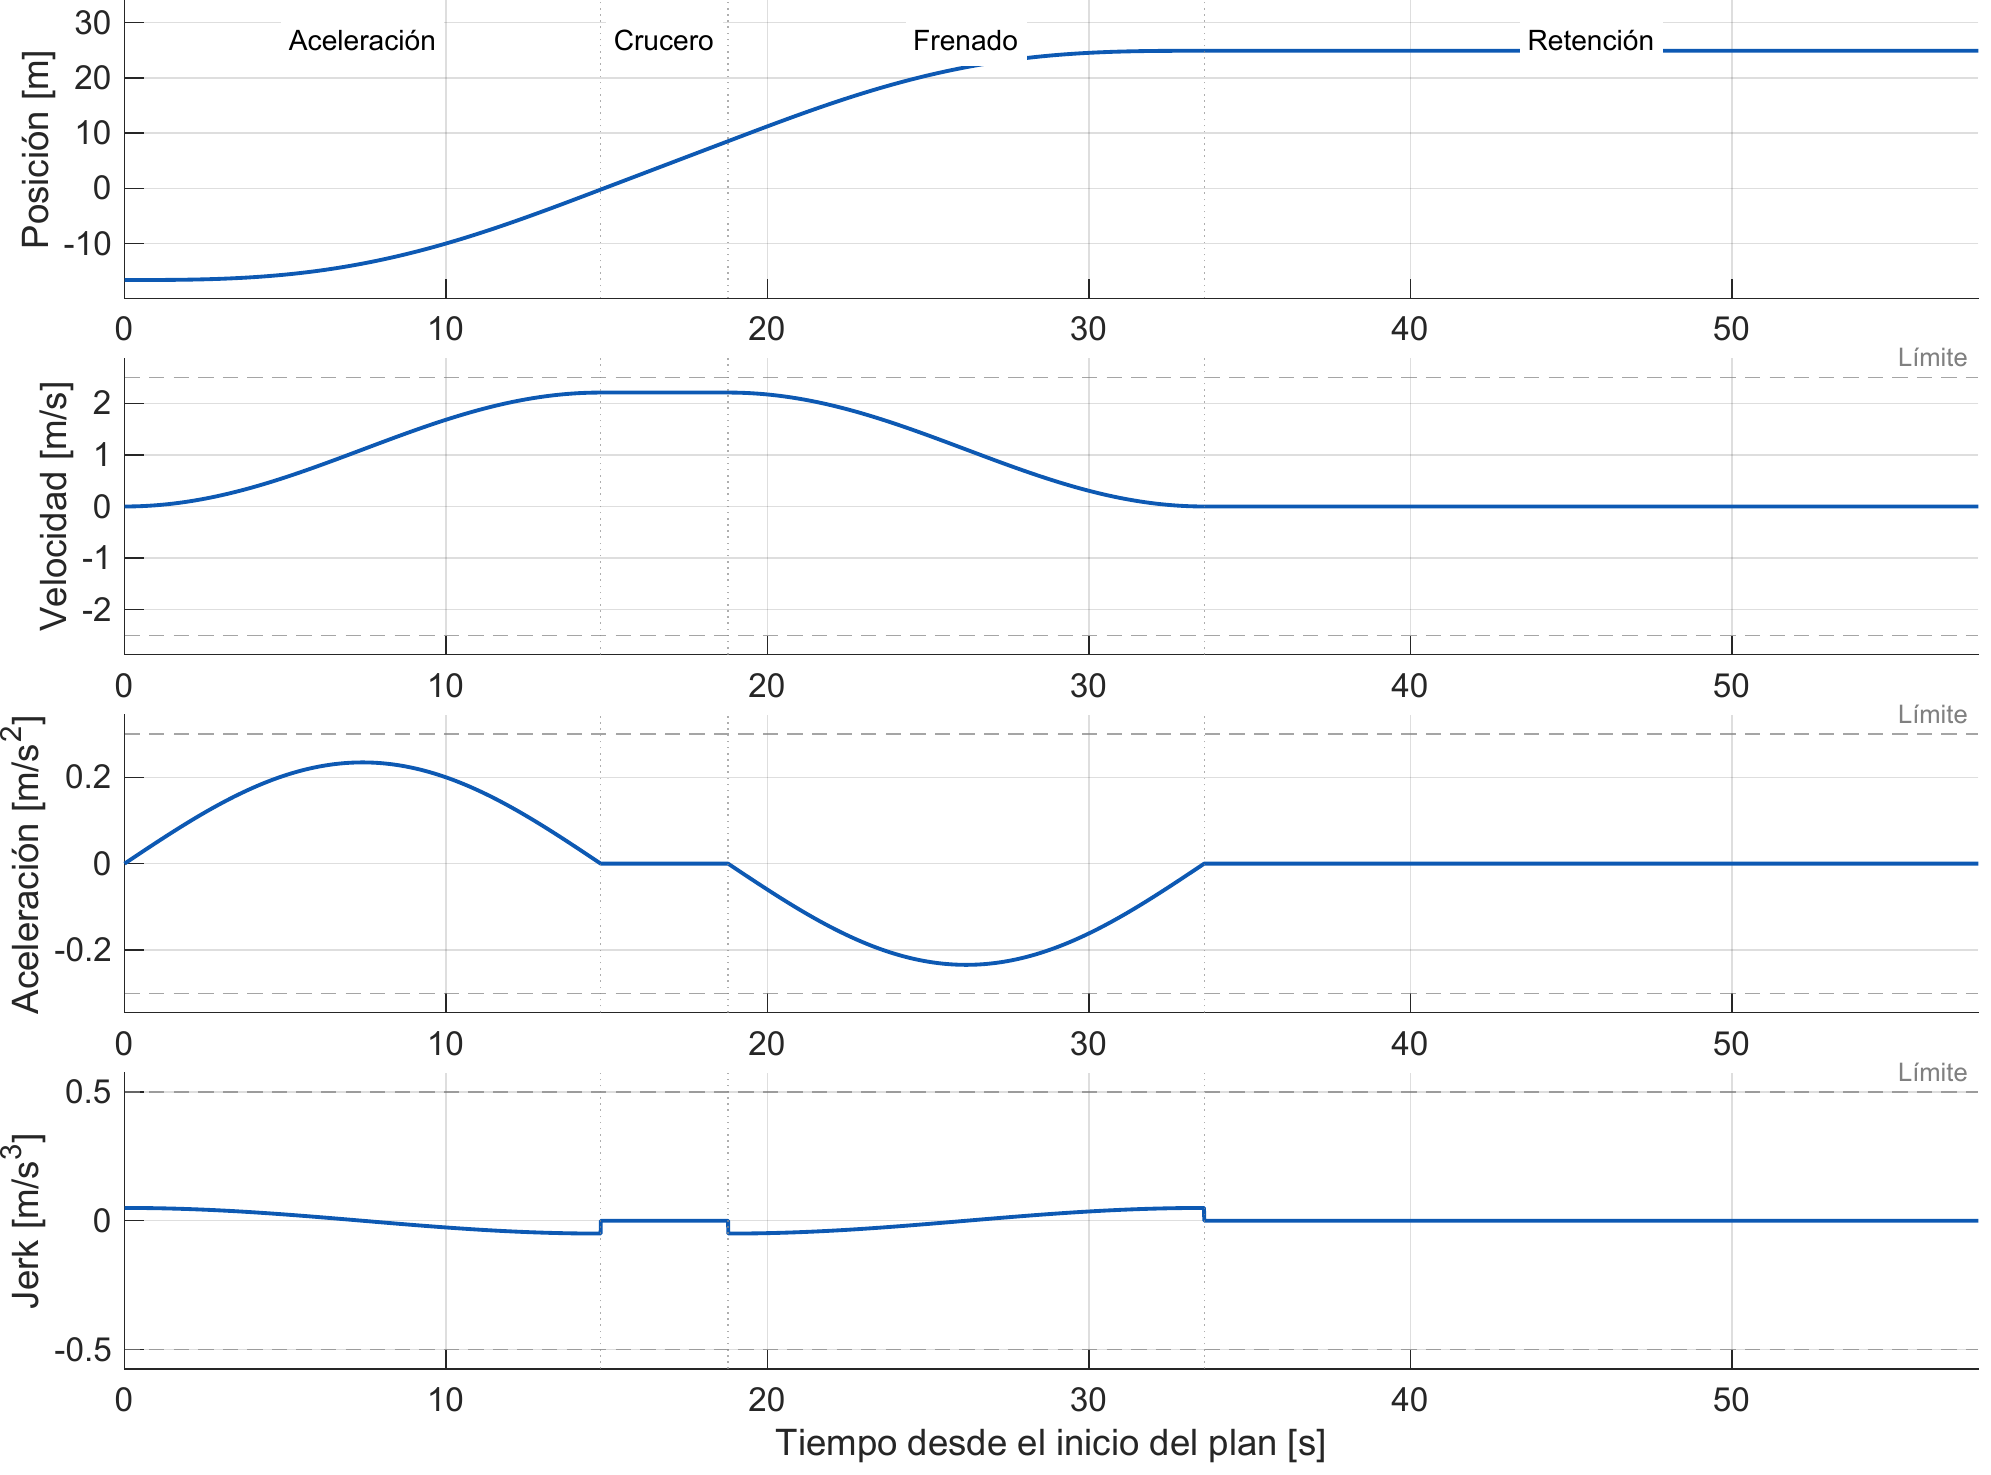
\includegraphics[width=.98\linewidth,height=5.55cm,keepaspectratio]{imagenes/r_023.png}\end{center}\vspace{-1mm}\figcaption{Slot 6 → 23; ejemplo de referencias sin respuesta de planta. $v_{x,max}=2,5$ m/s, $a_{x,max}=0,3$ m/s$^2$.}
\note{Identificar aceleración, crucero, frenado y retención. La velocidad de crucero disminuye si la distancia no permite alcanzar el máximo.}
\end{frame}
\begin{frame}[t,label=slide46]{Ejemplo del generador: referencia vertical}
\begin{center}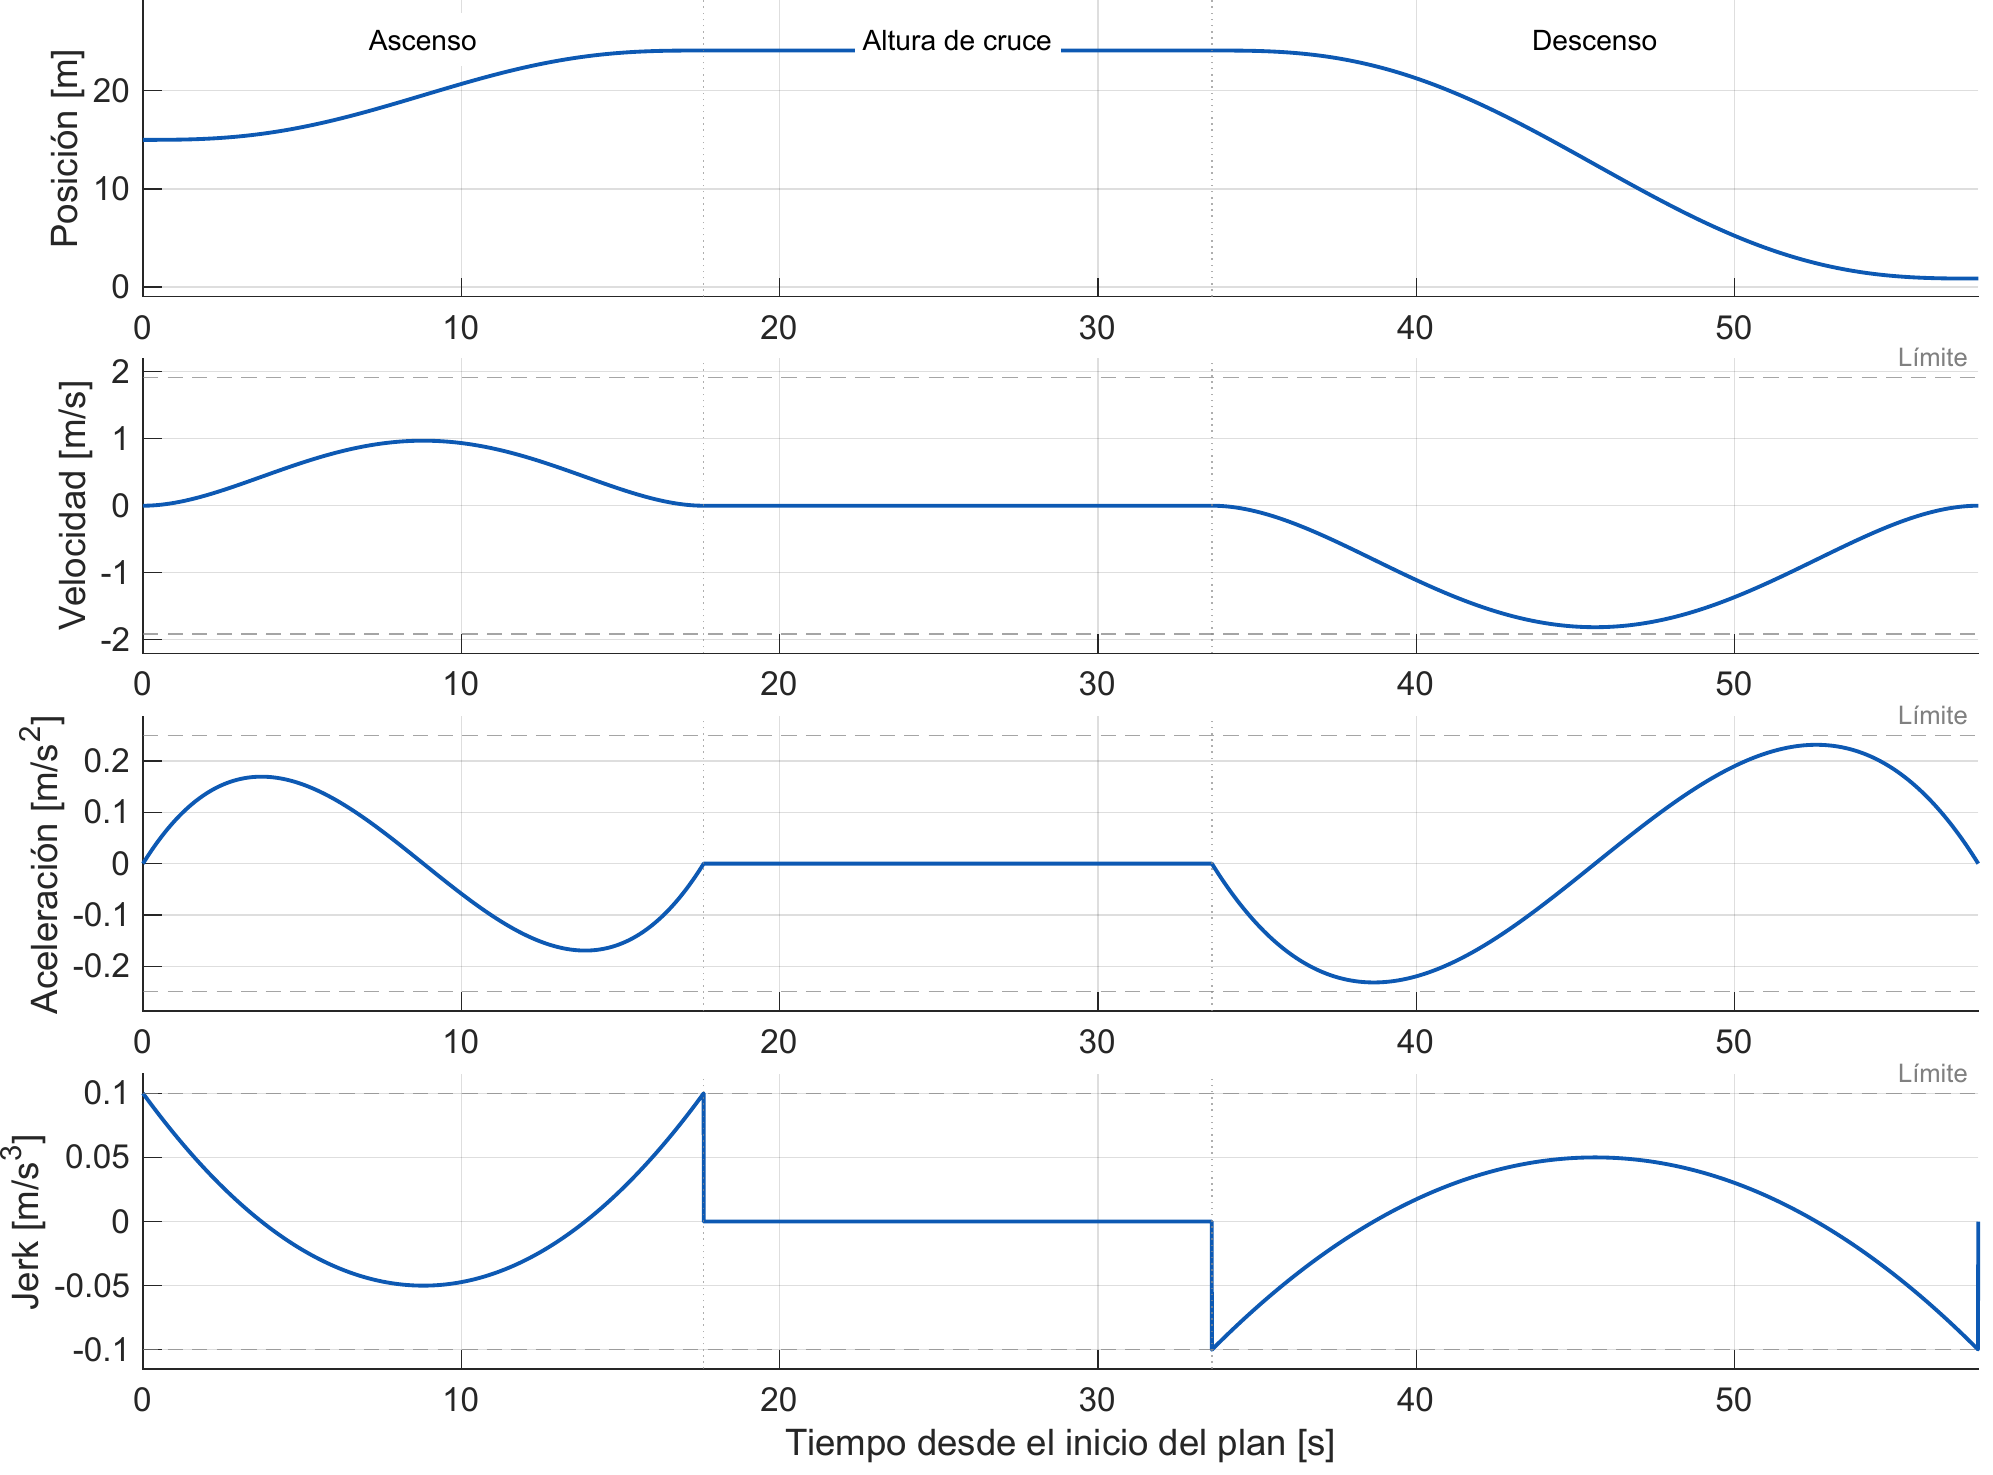
\includegraphics[width=.98\linewidth,height=5.55cm,keepaspectratio]{imagenes/r_024.png}\end{center}\vspace{-1mm}\figcaption{Ascenso, altura de cruce y descenso; trayectoria quíntica con límites de aceleración y jerk.}
\note{El ejemplo ilustra el planificador, no acredita cumplimiento físico de todos los límites de la guía. La velocidad vertical se configura además según masa y potencia.}
\end{frame}
\begin{frame}[t,label=slide47]{Coordinación sobre el perfil de obstáculos}
\begin{center}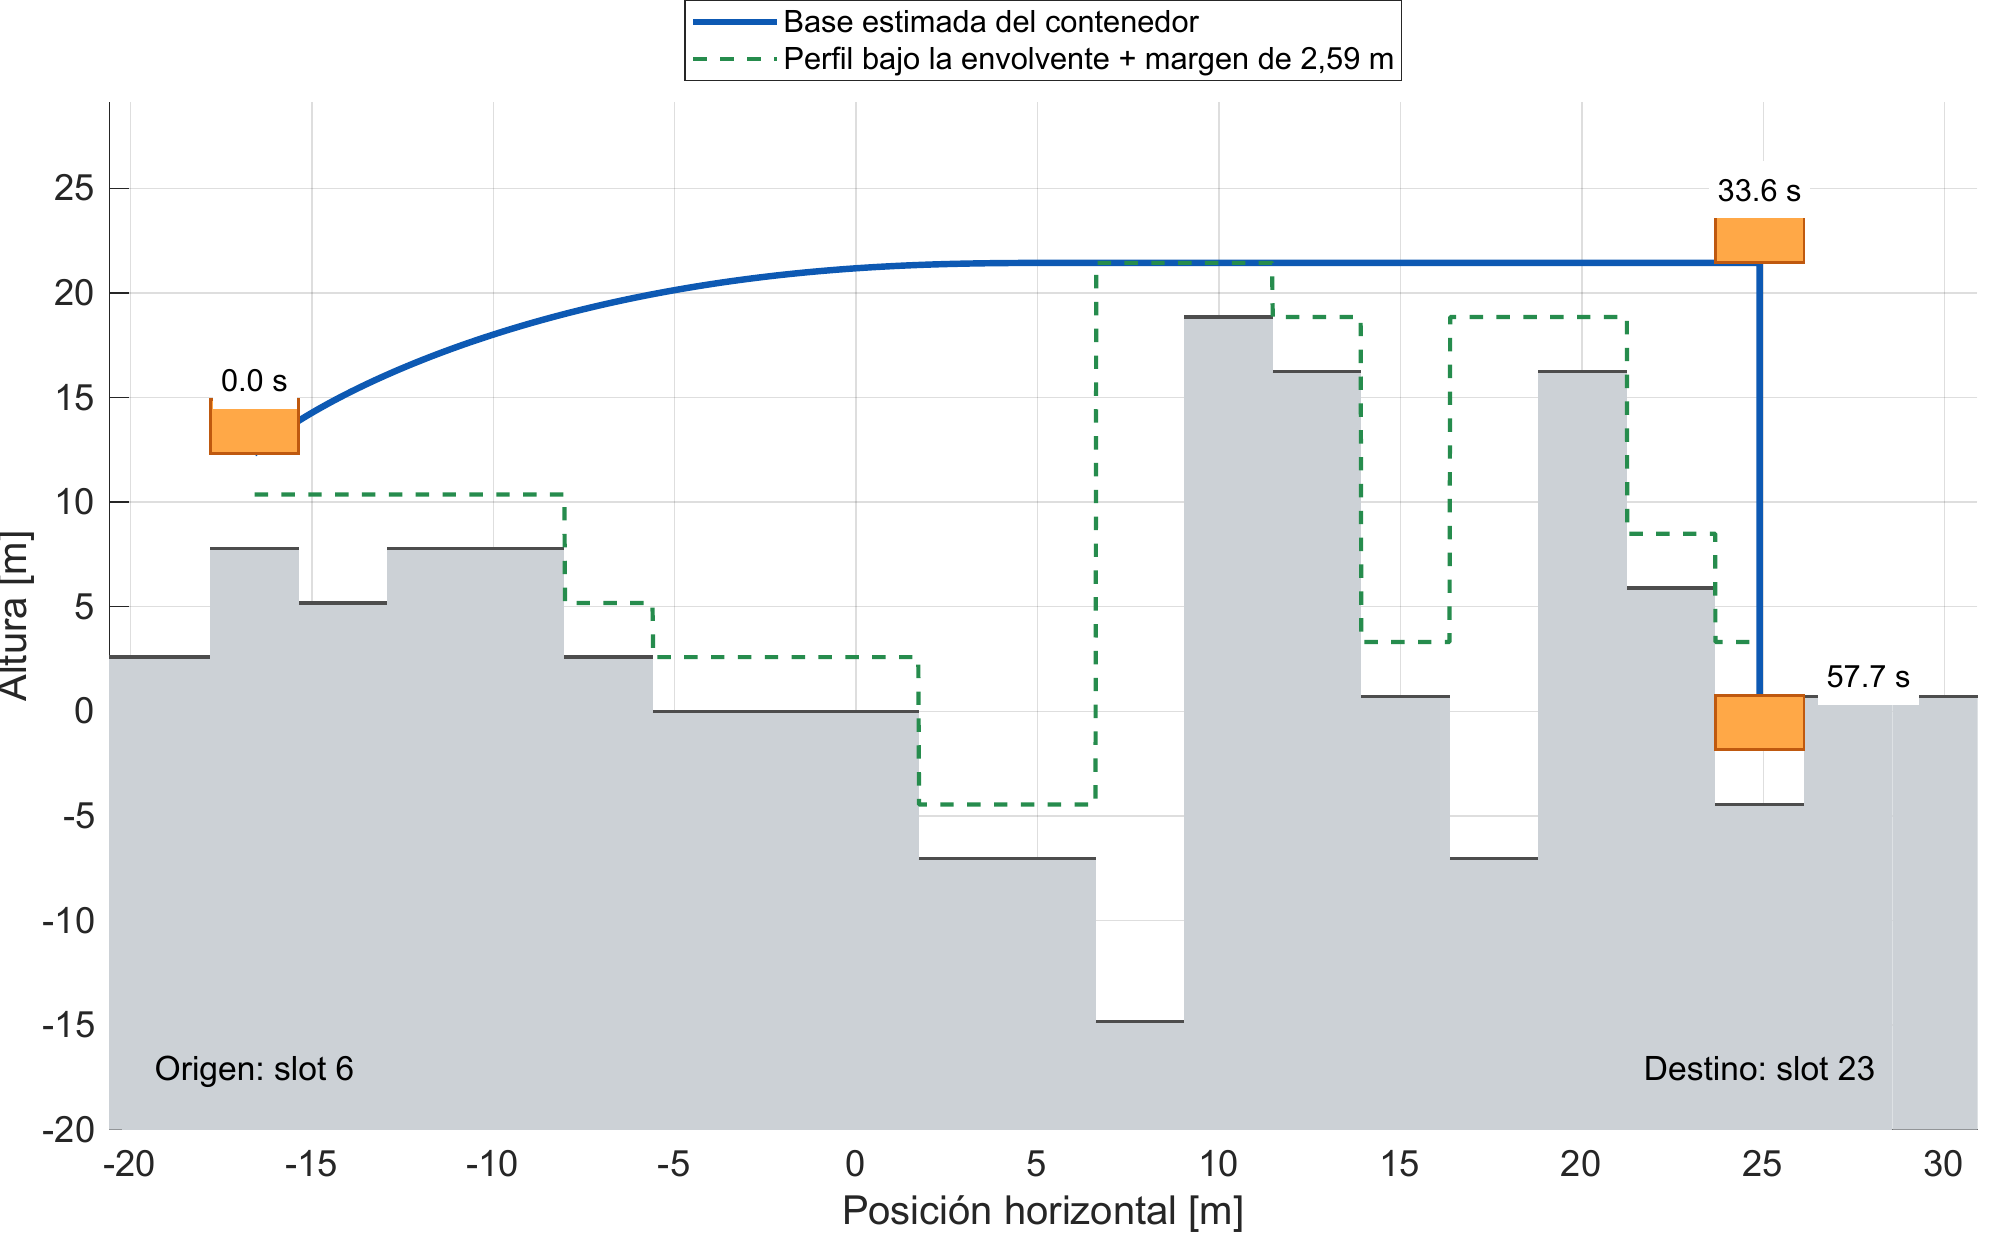
\includegraphics[width=.98\linewidth,height=5.55cm,keepaspectratio]{imagenes/r_025.png}\end{center}\vspace{-1mm}\figcaption{Ejemplo slot 6 → 23: plan de 57,66 s; sólo referencias generadas.}
\note{Recorrer el XY y explicar el alargamiento horizontal para dar tiempo al ascenso. No confundir estos 57,66 s con los traslados medidos en las pruebas completas.}
\end{frame}

\begin{frame}[t,label=cmp28]{Diagnóstico del supervisor · Stateflow}
\begin{center}\diagramfit{\begin{tikzpicture}
\node[sfstate] (ok) at (0,0) {DIAG OK\\Códigos nulos};
\node[sfstate] (alarm) at (5,0) {ALARMA\\Publica alarma};
\node[sfstate] (fault) at (10,0) {FALLA\\Publica falla};
\fill[accent](-1.8,0) circle(2pt);\draw[flow](-1.8,0)--(ok);
\draw[flow](ok)--node[guard,above,text width=2.3cm]{Sobrecarga}(alarm);
\draw[flow](alarm)--(fault);\node[guard,anchor=south,align=center,text width=3.6cm]at(7.5,.8){Seguimiento, carga\\o pérdida de permiso};
\draw[flow](ok.north)--++(0,1.55)-| (fault.north);
\node[guard,above,align=center] at (5,1.55){Seguimiento, carga o pérdida de permiso global};
\draw[flow](alarm.south)--++(0,-1.1)-|(ok.south);
\node[guard,below,align=center]at(2.5,-1.6){Reset y sin sobrecarga};
\draw[flow](fault.south)--++(0,-2.0)-|(ok.south);
\node[guard,below,align=center]at(5,-2.5){Reset, sin fallas y permiso global};
\end{tikzpicture}}\end{center}\vfill
{\small Diagnóstico exclusivo: OK, ALARMA o FALLA.\par}\vspace{1.5mm}{\fontsize{9.5}{11}\selectfont\textcolor{muted}{FALLA exige Reset, causas ausentes y permiso global. Una alarma puede evolucionar a falla.}\par}

\note{OK, ALARMA y FALLA son estados excluyentes. FALLA requiere reconocer la causa y recuperar el permiso. Una alarma de sobrecarga puede evolucionar a falla si aparece seguimiento fallido o pérdida de permiso.}
\end{frame}

\begin{frame}[t,label=cmp29]{Diagnóstico del supervisor · CODESYS SFC}
\begin{center}\diagramfit{\begin{tikzpicture}\begin{scope}[xshift=0.0cm]\node[font=\small\bfseries] at (1.5,.85){Alarma};
\node[sfcstep,double,double distance=1pt] (n0) at (0,0.0) {SIN ALARMA CARGA};
\node[sfcstep] (n1) at (0,-1.08) {ALARMA SOBRECARGA};
\draw[wire] (n0.south)--(n1.north);
\draw[wire,line width=1.1pt] (-.2,-0.54)--(.2,-0.54);
\node[guard,anchor=west,text width=3.4cm] at (1.85,-0.54) {Sobrecarga detectada};
\draw[flow] (n1.south)--(0,-1.73);
\node[guard,anchor=north,align=center,text width=5.4cm] at (1.6,-1.75) {Reset y sin sobrecarga: retorno a SIN ALARMA CARGA};
\end{scope}\begin{scope}[xshift=7.1cm]\node[font=\small\bfseries] at (1.5,.85){Falla};
\node[sfcstep,double,double distance=1pt] (n0) at (0,0.0) {SUPERVISOR OK};
\node[sfcstep] (n1) at (0,-1.08) {FALLO RETENIDO};
\draw[wire] (n0.south)--(n1.north);
\draw[wire,line width=1.1pt] (-.2,-0.54)--(.2,-0.54);
\node[guard,anchor=west,text width=3.4cm] at (1.85,-0.54) {Seguimiento, carga o permiso global ausente};
\draw[flow] (n1.south)--(0,-1.73);
\node[guard,anchor=north,align=center,text width=5.4cm] at (1.6,-1.75) {Reset, sin fallas y permiso global: retorno a SUPERVISOR OK};
\end{scope}\end{tikzpicture}}\end{center}\vfill
{\small Alarma de carga y falla de supervisor tienen memorias SFC independientes.\par}\vspace{1.5mm}{\fontsize{9.5}{11}\selectfont\textcolor{muted}{ST calcula los códigos y decide cuál publicar. El reconocimiento exige Reset y causas ausentes.}\par}

\note{Alarma de carga y falla de supervisor tienen memorias SFC independientes. ST calcula los códigos y decide cuál publicar. El reconocimiento exige Reset y causas ausentes. Los monitores pueden coexistir activos. El programa ST actual consulta la alarma antes de asignar el código de falla en su IF/ELSIF, por lo que la prioridad de publicación también requiere revisión al comparar implementaciones.}
\end{frame}

\begin{frame}[t,label=cmp30]{Tensión del cable e histéresis · Stateflow}
\begin{center}\diagramfit{\begin{tikzpicture}
\node[sfstate,text width=2.5cm] (n0) at (0.0,0) {CUERDA\\FLOJA};
\node[sfstate,text width=2.5cm] (n1) at (3.35,0) {CUERDA\\TENSA};
\draw[flow] (n0.east)--(n1.west);
\node[guard,text width=3.35cm,anchor=south] at (1.675,.78) {Tensión mayor\\que 15 kN};
\draw[flow] (n1.south)--++(0,-1.1) -| (n0.south);
\node[guard,anchor=north,align=center,text width=9cm] at (1.675,-1.6) {Tensión menor que 12 kN};
\end{tikzpicture}}\end{center}\vfill
{\small La memoria de histéresis evita alternar cuerda floja y tensa cerca de un único umbral.\par}\vspace{1.5mm}{\fontsize{9.5}{11}\selectfont\textcolor{muted}{Tensa por encima de 15 kN. Floja por debajo de 12 kN. Entre ambos valores conserva el estado.}\par}

\note{La memoria de histéresis evita alternar cuerda floja y tensa cerca de un único umbral. Tensa por encima de 15 kN. Floja por debajo de 12 kN. Entre ambos valores conserva el estado.}
\end{frame}

\begin{frame}[t,label=cmp31]{Tensión del cable e histéresis · CODESYS SFC}
\begin{center}\diagramfit{\begin{tikzpicture}
\node[sfcstep,double,double distance=1pt] (n0) at (0,0.0) {CUERDA FLOJA};
\node[sfcstep] (n1) at (0,-1.08) {CUERDA TENSA};
\draw[wire] (n0.south)--(n1.north);
\draw[wire,line width=1.1pt] (-.2,-0.54)--(.2,-0.54);
\node[guard,anchor=west,text width=8.7cm] at (1.85,-0.54) {Tensión mayor que 15 kN};
\draw[flow] (n1.south)--(0,-1.73);
\node[guard,anchor=north,align=center,text width=8.3cm] at (2.8,-1.75) {Tensión menor que 12 kN: salto a CUERDA FLOJA};
\end{tikzpicture}}\end{center}\vfill
{\small Dos pasos SFC implementan la memoria de tensión que Stateflow calcula en una función auxiliar.\par}\vspace{1.5mm}{\fontsize{9.5}{11}\selectfont\textcolor{muted}{La condición de cuerda tensa participa en el paso desde DESPEGUE SUAVE hacia PESAJE.}\par}

\note{Dos pasos SFC implementan la memoria de tensión que Stateflow calcula en una función auxiliar. La condición de cuerda tensa participa en el paso desde DESPEGUE SUAVE hacia PESAJE.}
\end{frame}

\section{Seguridad e interfaz}
\begin{frame}[plain,label=seccion6]
\setbeamertemplate{frametitle}{}
\vfill
{\fontsize{25}{29}\selectfont\bfseries Seguridad e interfaz de operación\par}
\vspace{4mm}\textcolor{accent}{\rule{.75\linewidth}{1pt}}\par\vspace{3mm}
{\large Permisos, protecciones y supervisión de la maniobra.\par}\vfill
\note{Ubicar este bloque en el recorrido y anunciar su objetivo.}
\end{frame}
\begin{frame}[t,label=slide49]{Protección independiente de la maniobra}
\begin{itemize}
\item Emergencias de carro, izaje y emergencia total.
\item Detección de límites, sobrevelocidad y pulsador.
\item Permisos por eje y autorizaciones de apertura de frenos.
\item Retención de emergencia hasta retirar causas y solicitar reinicio.
\item Watchdog de comunicación con vencimiento de 5 s.
\end{itemize}
\note{Explicar que independencia funcional no implica certificación de seguridad. En Stateflow las regiones de emergencias y watchdog se ejecutan en orden definido.}
\end{frame}
\begin{frame}[t,label=cmp32]{Organización de seguridad · Stateflow}
\begin{center}\diagramfit{\begin{tikzpicture}
\node[sfstate,dashed,text width=2.2cm] (n0) at (0.0,0) {SALTOS\\EMERGENCIAS};
\node[sfstate,dashed,text width=2.2cm] (n1) at (2.75,0) {WATCHDOG};
\node[guard,anchor=north,align=center] at (0.0,-.75) {Orden 1};
\node[guard,anchor=north,align=center] at (2.75,-.75) {Orden 2};
\end{tikzpicture}}\end{center}\vfill
{\small Seguridad se ejecuta independientemente de la planificación y los mandos de producción.\par}\vspace{1.5mm}{\fontsize{9.5}{11}\selectfont\textcolor{muted}{Primero evalúa SALTOS EMERGENCIAS y después WATCHDOG. El orden afecta la respuesta y el rearme.}\par}

\note{Seguridad se ejecuta independientemente de la planificación y los mandos de producción. Primero evalúa SALTOS EMERGENCIAS y después WATCHDOG. El orden afecta la respuesta y el rearme.}
\end{frame}

\begin{frame}[t,label=cmp33]{Organización de seguridad · CODESYS SFC}
\begin{center}\diagramfit{\begin{tikzpicture}
\node[sfcstep,double,double distance=1pt] (init) at (1.375,1.75){INICIAL};
\draw[wire](init.south)--(1.375,.82);
\draw[wire,line width=1pt](1.175,1.05)--(1.575,1.05);
\node[guard,anchor=west]at(1.725,1.05){TRUE};
\draw[wire,line width=1pt](-1.2,0.82)--(3.95,0.82);
\draw[wire,line width=1pt](-1.2,0.75)--(3.95,0.75);
\draw[wire,line width=1pt](-1.2,-0.75)--(3.95,-0.75);
\draw[wire,line width=1pt](-1.2,-0.82)--(3.95,-0.82);
\node[sfcstep,text width=2.2cm](r0)at(0.0,0){SALTOS\\EMERGENCIAS};
\draw[wire](0.0,.75)--(r0.north);
\draw[wire](r0.south)--(0.0,-.75);
\node[sfcstep,text width=2.2cm](r1)at(2.75,0){WATCHDOG};
\draw[wire](2.75,.75)--(r1.north);
\draw[wire](r1.south)--(2.75,-.75);
\node[sfcstep](stop)at(1.375,-1.8){DETENIDA};
\draw[wire](1.375,-.82)--(stop.north);
\draw[wire,line width=1pt](1.175,-1.05)--(1.575,-1.05);
\node[guard,anchor=west]at(1.725,-1.05){FALSE};
\node[guard,anchor=north,align=center]at(1.375,-2.3){TRUE: salto a INICIAL};
\end{tikzpicture}}\end{center}\vfill
{\small La tarea evalúa los monitores SFC y después arbitra las salidas en ST.\par}\vspace{1.5mm}{\fontsize{9.5}{11}\selectfont\textcolor{muted}{WATCHDOG precede a EMERGENCIA TOTAL para aplicar el timeout en la misma trama.}\par}

\note{El contenedor muestra dos ramas. La tarea llama primero a los monitores y luego arbitra las salidas en ST. El watchdog se evalúa antes de la emergencia total para que el timeout pueda intervenir en la misma trama.}
\end{frame}

\begin{frame}[t,label=cmp34]{Seguridad: emergencias por eje · Stateflow}
\begin{center}\diagramfit{\begin{tikzpicture}
\node[sfstate](ok)at(5,1.5){NORMAL};
\node[sfstate,text width=3cm](t)at(.5,-.6){EMERGENCIA CARRO\\BRK\_t = 0};
\node[sfstate,text width=3cm](h)at(9.5,-.6){EMERGENCIA IZAJE\\BRK\_h = BRK\_hE = 0};
\draw[flow](ok.west)-|(t.north);\draw[flow](ok.east)-|(h.north);
\node[guard,align=center,text width=3.2cm]at(1.5,2.3){Prioridad 3: flanco\\de límite horizontal};
\node[guard,align=center,text width=3.9cm]at(8.5,2.3){Prioridad 2: flanco de límite\\vertical o sobrevelocidad};
\draw[wire](t.south)--(.5,-1.65)--(9.5,-1.65)--(h.south);
\draw[flow](5,-1.65)--(ok.south);
\node[guard,align=center,text width=10cm]at(5,-2.2){Rearme: flanco de reinicio y desaparición de las causas};
\end{tikzpicture}}\end{center}\vfill
{\small Cada emergencia retira la autorización de apertura de freno del eje afectado.\par}\vspace{1.5mm}{\fontsize{9.5}{11}\selectfont\textcolor{muted}{Si ambos flancos coinciden desde NORMAL, la prioridad de Stateflow reconoce primero izaje.}\par}

\note{Cada emergencia retira la autorización de apertura de freno del eje afectado. Si ambos flancos coinciden desde NORMAL, la prioridad de Stateflow reconoce primero izaje.}
\end{frame}

\begin{frame}[t,label=cmp35]{Seguridad: emergencias por eje · CODESYS SFC}
\begin{center}\diagramfit{\begin{tikzpicture}\begin{scope}[xshift=0.0cm]\node[font=\small\bfseries] at (1.5,.85){Carro};
\node[sfcstep,double,double distance=1pt] (n0) at (0,0.0) {CARRO SEGURO};
\node[sfcstep] (n1) at (0,-1.08) {EMERGENCIA CARRO};
\draw[wire] (n0.south)--(n1.north);
\draw[wire,line width=1.1pt] (-.2,-0.54)--(.2,-0.54);
\node[guard,anchor=west,text width=3.4cm] at (1.85,-0.54) {Flanco de límite último horizontal};
\draw[flow] (n1.south)--(0,-1.73);
\node[guard,anchor=north,align=center,text width=5.4cm] at (1.6,-1.75) {Flanco de reset y límites ausentes: retorno a CARRO SEGURO};
\end{scope}\begin{scope}[xshift=7.1cm]\node[font=\small\bfseries] at (1.5,.85){Izaje};
\node[sfcstep,double,double distance=1pt] (n0) at (0,0.0) {IZAJE SEGURO};
\node[sfcstep] (n1) at (0,-1.08) {EMERGENCIA IZAJE};
\draw[wire] (n0.south)--(n1.north);
\draw[wire,line width=1.1pt] (-.2,-0.54)--(.2,-0.54);
\node[guard,anchor=west,text width=3.4cm] at (1.85,-0.54) {Flanco de límite vertical o sobrevelocidad};
\draw[flow] (n1.south)--(0,-1.73);
\node[guard,anchor=north,align=center,text width=5.4cm] at (1.6,-1.75) {Flanco de reset, límites y sobrevelocidad ausentes: retorno a IZAJE SEGURO};
\end{scope}\end{tikzpicture}}\end{center}\vfill
{\small Los dos monitores SFC pueden reconocer emergencias de carro e izaje en la misma trama.\par}\vspace{1.5mm}{\fontsize{9.5}{11}\selectfont\textcolor{muted}{El rearme exige un nuevo flanco de Reset y que los sensores del eje hayan dejado de indicar peligro.}\par}

\note{Los dos monitores SFC pueden reconocer emergencias de carro e izaje en la misma trama. El rearme exige un nuevo flanco de Reset y que los sensores del eje hayan dejado de indicar peligro.}
\end{frame}

\begin{frame}[t,label=cmp36]{Seguridad: emergencia total · Stateflow}
\begin{center}\diagramfit{\begin{tikzpicture}
\node[sfstate,text width=2.5cm] (n0) at (0.0,0) {NORMAL O\\EMERGENCIA PARCIAL};
\node[sfstate,text width=2.5cm] (n1) at (3.35,0) {EMERGENCIA\\TOTAL};
\fill[accent] (-1.8,0) circle (2pt);
\draw[flow] (-1.8,0)--(n0.west);
\draw[flow] (n0.east)--(n1.west);
\node[guard,text width=3.35cm,anchor=south] at (1.675,.78) {Pulsador, watchdog\\o escalamiento desde parcial};
\draw[flow] (n1.south)--++(0,-1.1) -| (n0.south);
\node[guard,anchor=north,align=center,text width=9cm] at (1.675,-1.6) {Todas las causas ausentes y flanco de reinicio};
\end{tikzpicture}}\end{center}\vfill
{\small Pulsador, watchdog o escalamiento desde una emergencia parcial retiran las tres autorizaciones.\par}\vspace{1.5mm}{\fontsize{9.5}{11}\selectfont\textcolor{muted}{Reset sólo devuelve a NORMAL cuando desaparecieron todas las causas y los límites están libres.}\par}

\note{Pulsador, watchdog o escalamiento desde una emergencia parcial retiran las tres autorizaciones. Reset sólo devuelve a NORMAL cuando desaparecieron todas las causas y los límites están libres.}
\end{frame}

\begin{frame}[t,label=cmp37]{Seguridad: emergencia total · CODESYS SFC}
\begin{center}\diagramfit{\begin{tikzpicture}
\node[sfcstep,double,double distance=1pt] (n0) at (0,0.0) {SEGURIDAD NORMAL};
\node[sfcstep] (n1) at (0,-1.08) {EMERGENCIA TOTAL};
\draw[wire] (n0.south)--(n1.north);
\draw[wire,line width=1.1pt] (-.2,-0.54)--(.2,-0.54);
\node[guard,anchor=west,text width=8.7cm] at (1.85,-0.54) {Pulsador, falla OPC UA, watchdog o emergencias de ambos ejes};
\draw[flow] (n1.south)--(0,-1.73);
\node[guard,anchor=north,align=center,text width=8.3cm] at (2.8,-1.75) {Reset y desaparición de todas las causas: retorno a SEGURIDAD NORMAL};
\end{tikzpicture}}\end{center}\vfill
{\small La emergencia total incorpora pulsador, watchdog, falla OPC UA y coexistencia de emergencias de ambos ejes.\par}\vspace{1.5mm}{\fontsize{9.5}{11}\selectfont\textcolor{muted}{La salida ST anula permisos y órdenes de movimiento hasta el reconocimiento y la desaparición de las causas.}\par}

\note{La emergencia total incorpora pulsador, watchdog, falla OPC UA y coexistencia de emergencias de ambos ejes. La salida ST anula permisos y órdenes de movimiento hasta el reconocimiento y la desaparición de las causas.}
\end{frame}

\begin{frame}[t,label=cmp38]{Seguridad: watchdog · Stateflow}
\begin{center}\diagramfit{\begin{tikzpicture}
\node[sfstate,text width=2.5cm] (n0) at (0.0,0) {NORMAL};
\node[sfstate,text width=2.5cm] (n1) at (3.35,0) {FALLO WD};
\fill[accent] (-1.8,0) circle (2pt);
\draw[flow] (-1.8,0)--(n0.west);
\draw[flow] (n0.east)--(n1.west);
\node[guard,text width=3.35cm,anchor=south] at (1.675,.78) {Sin cambios del pulso\\durante 5 s};
\draw[flow] (n1.south)--++(0,-1.1) -| (n0.south);
\node[guard,anchor=north,align=center,text width=9cm] at (1.675,-1.6) {Flanco de reinicio; un cambio de pulso reinicia el temporizador};
\end{tikzpicture}}\end{center}\vfill
{\small Cada cambio de pulso reinicia la espera. Sin cambios durante 5 s dispara FALLO WD.\par}\vspace{1.5mm}{\fontsize{9.5}{11}\selectfont\textcolor{muted}{Reset rearma el monitor. La emergencia total puede necesitar otro flanco.}\par}

\note{Cada cambio del pulso reinicia la espera. Sin cambios durante el tiempo máximo se memoriza FALLO WD. El flanco de Reset rearma el monitor. La emergencia total se evalúa antes y puede requerir otro flanco. El cambio del pulso es una autotransición que reinicia la temporización del estado NORMAL. SALTOS EMERGENCIAS se evalúa antes que WATCHDOG.}
\end{frame}

\begin{frame}[t,label=cmp39]{Seguridad: watchdog · CODESYS SFC}
\begin{center}\diagramfit{\begin{tikzpicture}
\node[sfcstep,double,double distance=1pt] (n0) at (0,0.0) {WATCHDOG OK};
\node[sfcstep] (n1) at (0,-1.08) {WATCHDOG DISPARADO};
\draw[wire] (n0.south)--(n1.north);
\draw[wire,line width=1.1pt] (-.2,-0.54)--(.2,-0.54);
\node[guard,anchor=west,text width=8.7cm] at (1.85,-0.54) {Sin cambios del pulso durante 5 s};
\draw[flow] (n1.south)--(0,-1.73);
\node[guard,anchor=north,align=center,text width=8.3cm] at (2.8,-1.75) {Flanco de reset y timeout ausente: salto a WATCHDOG OK};
\end{tikzpicture}}\end{center}\vfill
{\small ST mide el tiempo sin cambios del pulso y el SFC conserva el estado de watchdog disparado.\par}\vspace{1.5mm}{\fontsize{9.5}{11}\selectfont\textcolor{muted}{El rearme exige flanco de Reset y timeout ausente. Son 5 s simulados en este banco.}\par}

\note{ST mide el tiempo sin cambios del pulso y el SFC conserva el estado de watchdog disparado. El rearme exige flanco de Reset y timeout ausente. Son 5 s simulados en este banco.}
\end{frame}





\begin{frame}[t,label=slide50]{Pruebas aisladas de seguridad: 25 escenarios}
\begin{center}
{\small\renewcommand{\arraystretch}{1.0}
\begin{tabular}{p{4.4cm}p{9.3cm}}\toprule
Caso & Resultado observado\\\midrule
Retención y reinicio & Emergencia enclavada; rearme por flanco\\
Fallas sucesivas & Escalamiento a emergencia total\\
Fallas simultáneas & Prevalece izaje; carro conserva permiso\\
Límite activo desde arranque & Puede no detectar por esperar flanco\\
Watchdog & 5 s + un ciclo; recuperación con dos flancos\\
\bottomrule\end{tabular}}\end{center}

\note{Las entradas fueron programadas a 20 ms y se verificaron salidas lógicas. No se ensayaron distancias físicas de detención frente a una falla integrada.}
\end{frame}
\begin{frame}[t,label=slide51]{Visualización e interfaz HMI}
\relax
\figurefooter{Representación de carga, perfil, envolvente local, línea de cruce y estados operativos.}
\vspace{-2mm}\makebox[\linewidth][c]{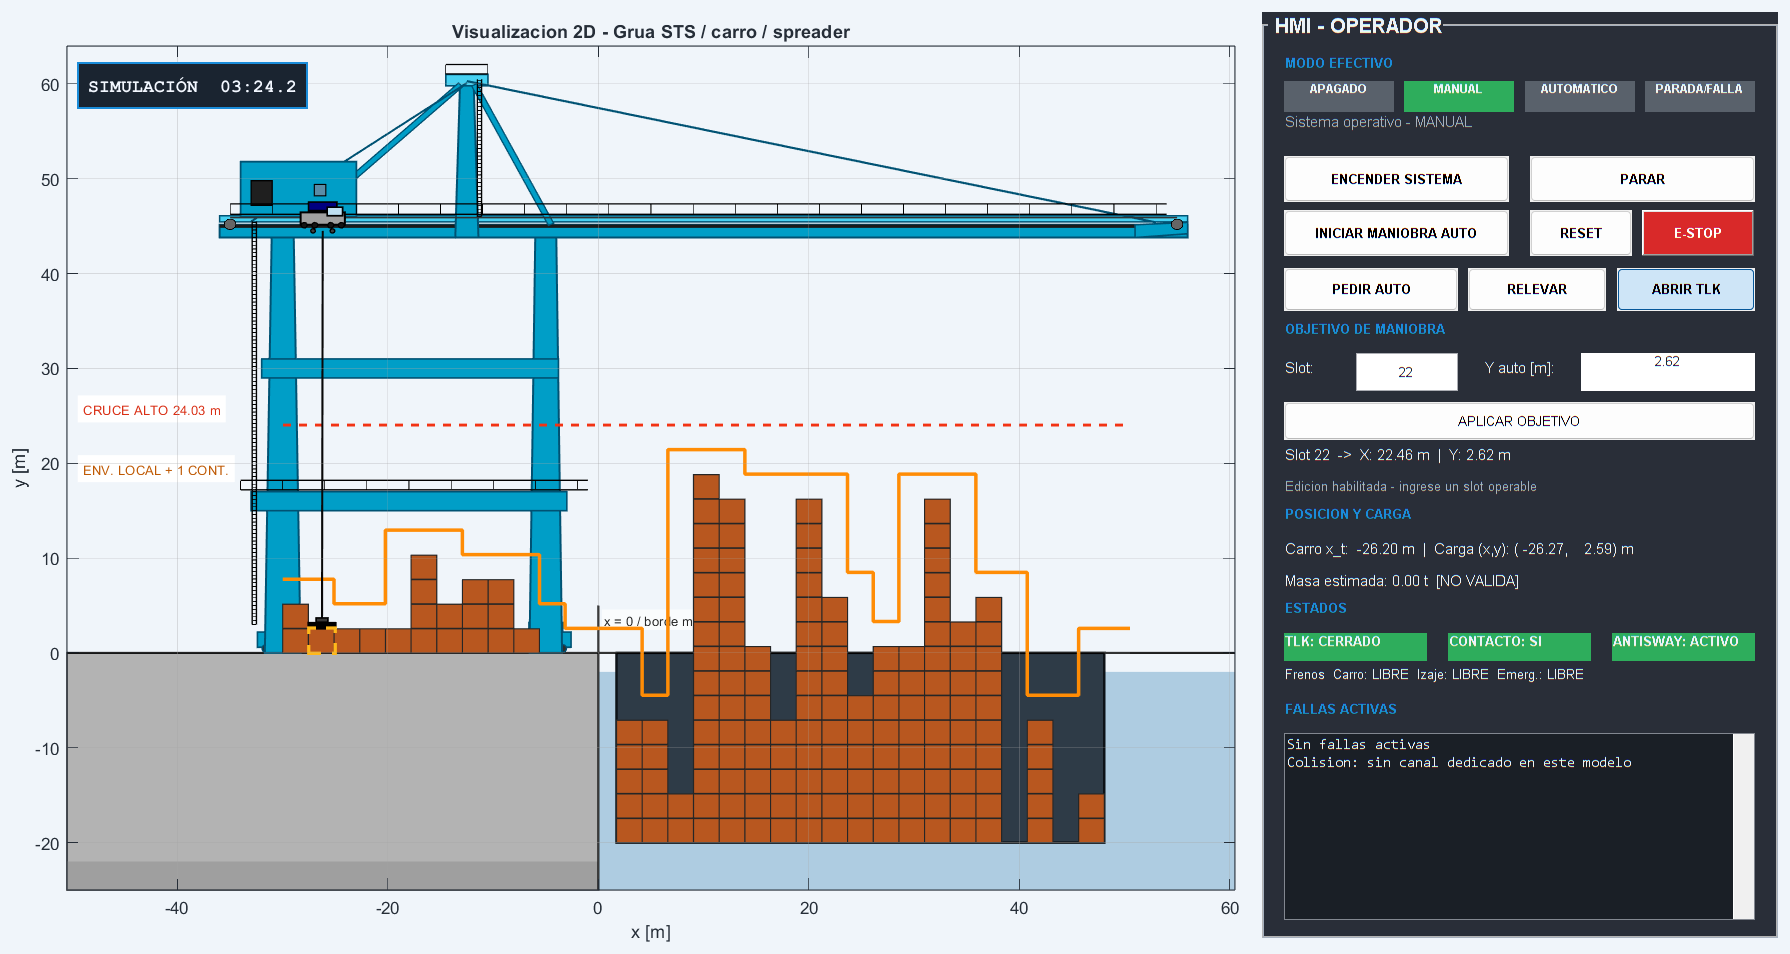
\includegraphics[width=15.0cm,height=6.05cm,keepaspectratio,trim=7.00bp 7.00bp 7.00bp 7.00bp,clip]{imagenes/r_038.png}}\par\note{Mostrar mandos manuales, selección de objetivo y solicitud de modos. La HMI sirve para operar y observar la simulación; los videos se reproducirán desde archivos.}
\end{frame}
\section{CODESYS y Motion Controller}
\begin{frame}[plain,label=seccion7]
\setbeamertemplate{frametitle}{}
\vfill
{\fontsize{25}{29}\selectfont\bfseries Implementación en CODESYS y Motion Controller\par}
\vspace{4mm}\textcolor{accent}{\rule{.75\linewidth}{1pt}}\par\vspace{3mm}
{\large Ejecución de la lógica y realización discreta de los reguladores.\par}\vfill
\note{Ubicar este bloque en el recorrido y anunciar su objetivo.}
\end{frame}
\begin{frame}[t,label=slide52]{Co-simulación de planta y autómatas}

\begin{center}\begin{tikzpicture}[node distance=14mm,every node/.style={font=\small},b/.style={draw=accent,text width=5cm,minimum height=25mm,align=center},a/.style={<->,thick}]
\node[b](sl){MATLAB / Simulink\\Planta, sensores, MC y HMI};\node[b,right=of sl](plc){CODESYS\\Supervisor y seguridad};\draw[a](sl)--node[above]{OPC UA}(plc);
\end{tikzpicture}\end{center}
\begin{itemize}\item Regulación a 1 ms; tarea PLC a 20 ms.
\item Referencias y permisos enviados a Simulink; mediciones enviadas al PLC.
\item Ensayos finales sincronizados por tramas de tiempo simulado.
\item Vigilancia del enlace independiente del avance de la maniobra.\end{itemize}

\note{Explicar por qué una tarea periódica y una simulación acelerada no quedan sincronizadas sólo por compartir una conexión OPC UA. El banco final coordina tramas.}
\end{frame}
\begin{frame}[t,label=slide53]{Implementaciones PLC: SFC manual y ST generado}
\begin{center}{\small\renewcommand{\arraystretch}{1.1}
\begin{tabular}{p{3cm}p{5.1cm}p{5.1cm}}\toprule
Aspecto & CODESYS manual & CODESYS automático\\\midrule
Secuencia & Pasos y transiciones SFC & Estados y transiciones en ST\\
Acciones & Programas ST consultan pasos activos & Bloques generados conservan memoria\\
Temporización & Acumuladores de 20 ms simulados & Contadores y planificador adaptados\\
Depuración & Paso activo y guardas & Estado interno y señales del FB\\
Planta & Simulink mediante OPC UA & Simulink mediante OPC UA\\\bottomrule
\end{tabular}}\end{center}\vfill
Ambas versiones ejecutan supervisor y seguridad en el PLC. La regulación y la planta siguen en Simulink.
\note{No confundir programación manual con conducción manual de la grúa. Ambas versiones combinan manual y automático, pero las estructuras internas no son idénticas.}
\end{frame}
\begin{frame}[t,label=slide54]{Aspectos críticos de la migración}
\begin{itemize}
\item Stateflow combina regiones paralelas, jerarquía y acciones de entrada, permanencia y salida.
\item SFC expresa la secuencia. ST reproduce cálculos, memorias e interbloqueos.
\item PLC Coder traduce la memoria de los charts a bloques funcionales ST.
\item La interfaz debe conservar tipos, dimensiones, inicialización y orden de ejecución.
\item Igualar los periodos exige revisar cuándo se evalúa cada transición.
\end{itemize}\vfill
{\small La comparación debe verificar las órdenes y las recuperaciones, además de la secuencia nominal.}
\note{La implementación manual de CODESYS anula permisos globales y de ambos ejes ante emergencias parciales, a diferencia del OR global de Stateflow. Los monitores paralelos reconocen eventos simultáneos de forma diferente.}
\end{frame}
\begin{frame}[t,label=slide55]{Temporizaciones: adaptar la base de ejecución}
\begin{center}
{\small\renewcommand{\arraystretch}{1.0}
\begin{tabular}{p{4.6cm}p{4.6cm}p{4.5cm}}\toprule
Código exportado & Ejecución sin ajustar & Adaptación aplicada\\\midrule
Base 1 ms; divisor 20 & 400 ms a tarea de 20 ms & Umbral 19 → 0\\
Base 1 ms; divisor 40 & 800 ms a tarea de 20 ms & Umbral 39 → 1\\
\bottomrule\end{tabular}}\end{center}
\begin{itemize}
\item Un divisor interno de 20 invocaciones sobre una tarea de 20 ms produce 400 ms.
\item El banco avanza un paso por trama de 20 ms simulados y mantiene una vigilancia independiente del enlace.
\end{itemize}
\note{Explicar el contador y su evaluación; el número de invocaciones cambia al ejecutar una exportación con base 1 ms en una tarea de 20 ms.}
\end{frame}
\begin{frame}[t,label=slide56]{Motion Controller de dos ejes}
\relax
\figurefooter{Tres funciones: estimadores, MC Carro y MC Izaje; ejecución a 1 ms.}
\vspace{-2mm}\makebox[\linewidth][c]{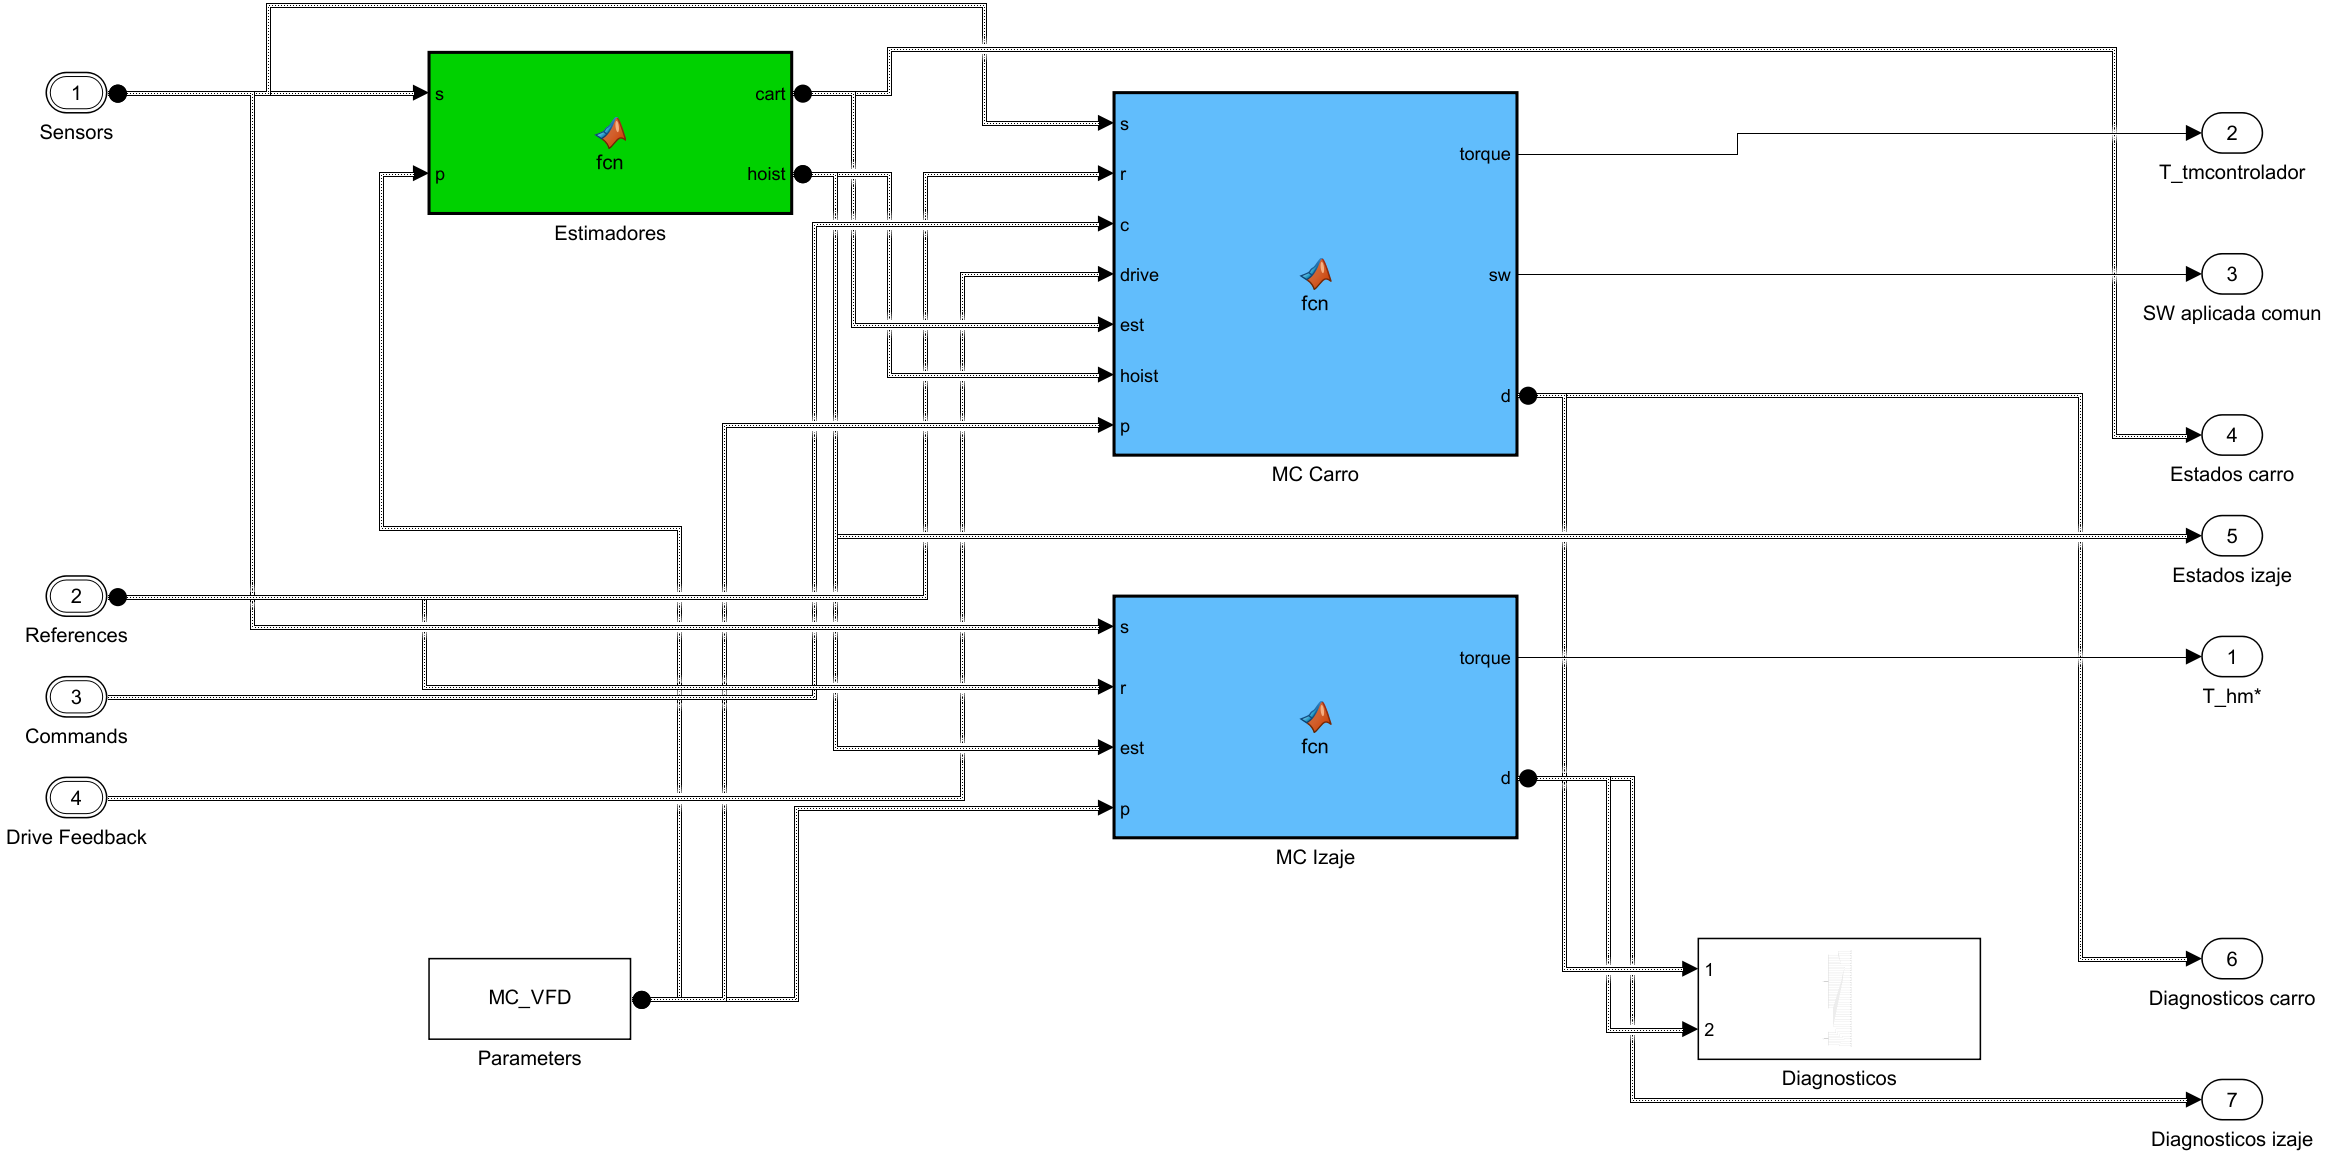
\includegraphics[width=15.0cm,height=6.05cm,keepaspectratio,trim=2.00bp 2.00bp 1.00bp 0.00bp,clip]{imagenes/r_060.png}}\par\note{El MC es una distribución funcional de software emulada en Simulink. No se seleccionó ni validó hardware industrial específico.}
\end{frame}
\begin{frame}[t,label=mcinterfaces]{MC: interfaces y orden de ejecución}
\begin{itemize}
\item \textbf{Entradas de medición:} encoders de motor, ángulo de carga y tensión del cable.
\item \textbf{Entradas del supervisor:} posición, velocidad y aceleración de ambos ejes, habilitaciones y órdenes de freno.
\item \textbf{Estimadores:} convierten coordenadas y actualizan velocidades antes de evaluar los reguladores.
\item \textbf{MC Carro / MC Izaje:} calculan torque solicitado y señales de diagnóstico cada 1 ms.
\item \textbf{Accionamientos:} aplican permisos, límites y dinámica de torque. El recorte retorna al anti-windup con 1 ms de demora.
\end{itemize}
\note{El MC es una unidad funcional emulada mediante tres MATLAB Function. Los estimadores separados evitan una dependencia artificial de las referencias. No implica una selección ni validación de hardware comercial.}
\end{frame}

\begin{frame}[t,label=slide57]{MC: estados y actualización de los estimadores}
\relax
\small Los estimadores continuos presentados antes de las pruebas se ejecutan con $T_s=1$ ms. Cada eje conserva sus estados y el encoder anterior.
\[\boldsymbol z=[\hat q\;\hat\omega]^T,\qquad u=\theta_m/i\]
\[\dot{\boldsymbol z}=A\boldsymbol z+Bu\]
\[A=\begin{bmatrix}-2\zeta_o\omega_o&1\\-\omega_o^2&0\end{bmatrix},\qquad
B=\begin{bmatrix}2\zeta_o\omega_o\\\omega_o^2\end{bmatrix}\]
\begin{itemize}
\item Coeficientes discretos calculados una vez en configuración.
\item Actualización mediante productos y sumas; sin derivar directamente muestras.
\item Posición convertida del encoder; velocidad obtenida de $\hat\omega$.
\end{itemize}
\note{Este bloque desarrolla la realización, no vuelve a introducir el estimador desde cero. Mantener el mismo nombre de los estados que en el bloque previo a pruebas. Referencias del supervisor retenidas entre actualizaciones de 20 ms. En la primera muestra se almacena el encoder y se conserva velocidad cero, conforme al código.}
\end{frame}
\begin{frame}[t,label=mcobservadores]{MC: actualización discreta de los observadores}
\[
\dot{\boldsymbol z}=A\boldsymbol z+Bu,\quad \boldsymbol z=[\hat q\;\hat\omega]^T,\quad u=\theta_m/i
\]
{\small
\[
A_d=(I-T_sA/2)^{-1}(I+T_sA/2),\qquad B_d=(I-T_sA/2)^{-1}T_sB/2
\]
\[
\boldsymbol z[n]=A_d\boldsymbol z[n-1]+B_d(u[n-1]+u[n])
\]
}
\begin{itemize}
\item Coeficientes calculados en configuración. Cada muestra ejecuta productos y sumas.
\item Estados y encoder anterior quedan en memoria persistente.
\item Inicialización coherente con velocidad cero. Polos discretos de módulo $0{,}960784<1$.
\end{itemize}
\note{Tustin con wn=40 rad/s y zeta=1. La posición se obtiene directamente del encoder, no del estado q. El estado w estima velocidad angular.}
\end{frame}
\begin{frame}[t,label=mccarro]{MC del carro: integración y anti-windup}
\relax\setlength{\parskip}{0pt}\setlength{\abovedisplayskip}{3pt}\setlength{\belowdisplayskip}{3pt}
\small\setlength{\abovedisplayskip}{3pt}\setlength{\belowdisplayskip}{3pt} $T_s=1$ ms. Los recortes de aceleración y torque de la muestra anterior corrigen el integrador.
\[K_{Ta}=\frac{r_{td}M_{EQt}}{i_t},\qquad
u_I[n]=e_v[n]+\frac{\Delta a[n-1]+\Delta T[n-1]/K_{Ta}}{K_{iv}T_{aw}}\]
\[I_v[n]=\operatorname{sat}_{I_{max}}\!\left(X[n]+\frac{T_s}{2}u_I[n]\right)\]
\[X[n+1]=\operatorname{sat}_{I_{max}}\!\left(I_v[n]+\frac{T_s}{2}u_I[n]\right)\]
\[I_{max}=a_{max}/K_{iv},\qquad T_{aw}=1\ \mathrm{s}\]
\begin{itemize}
\item Dos medios pasos Tustin: se limitan salida integral y memoria interna.
\item $\Delta a=a_c-a_u$; $\Delta T=T_{lim}-T_{in}$ antes de la dinámica del motor.
\item $X[n]$ y $\Delta a[n-1]$ permanecen entre muestras.
\end{itemize}
\note{Ecuaciones contrastadas con controlador_carro_mc_r2. No reemplazar los dos medios pasos limitados por una suma trapezoidal única: cambiaría salida y memoria al saturar. El torque recortado se entrega con demora de una muestra. La relación de anti-windup tiene Taw=1 s en el código. El regulador no recibe modo ni reset de eje: las autorizaciones se aplican fuera de este cálculo.}
\end{frame}
\begin{frame}[t,label=mccarrotorque]{MC del carro: cascada y salida de torque}
\relax
\small
\[e_x[n]=x_{ref}[n]-\hat x_t[n],\qquad \hat v_t[n]=r_{td}\hat\omega_{td}[n]\]
\[v_c[n]=\operatorname{sat}_{v_{max}}\!\left(v_{base}[n]+K_xe_x[n]\right)\]
\[e_v[n]=v_c[n]-\hat v_t[n]\]
\[a_u[n]=a_{ref}[n]+K_{pv}e_v[n]+K_{iv}I_v[n]\]
\[a_c[n]=\operatorname{sat}_{a_{max}}(a_u[n])\]
\[\boxed{T_{tm}^*[n]=\frac{r_{td}}{i_t}\left(M_{EQt}a_c[n]+b_{EQt}\hat v_t[n]-2F_w[n]\sin\theta_l[n]\right)}\]
\figcaption{$v_{base}$ es la entrada común de velocidad, que reúne referencia y correcciones. La salida es torque solicitado; permisos y capacidad del accionamiento se aplican a continuación.}
\note{Mantener v_base como frontera de entrada del regulador para posponer la definición de swTransfer, según acuerdo con el usuario. No se modifica ni se elimina esa señal del código. La ecuación final reproduce el cálculo de torque del MC: aceleración, rozamiento y fuerza pendular. La forma matemática se mantiene alineada con la diapositiva inicial de cascada; aquí Iv se obtiene de la realización discreta con anti-windup.}
\end{frame}
\begin{frame}[t,label=mcizaje]{MC Izaje: doble integración y torque}
\[
v_{l,ref}=-v_{h,ref},\quad a_{l,ref}=-a_{h,ref},\quad e_h=v_{l,ref}-\widehat{\dot l_h}
\]
{\small
\[
z_1[n]=z_1[n-1]+\frac{T_s}{2}(e_h[n-1]+e_h[n])
\]
\[
z_2[n]=z_2[n-1]+\frac{T_s}{2}(z_1[n-1]+z_1[n])
\]
\[
T_h^*=K_{hd}e_h+K_{hp}z_1+K_{hi}z_2
-\frac{r_{hd}}{i_h}(M_{EQh}a_{l,ref}+b_{EQh}v_{l,ref})+\frac{r_{hd}}{i_h}F_w
\]
}
\small El código conserva integrales, signos y condiciones iniciales. El supervisor sigue resolviendo frenos, pesaje y transferencia de carga.
\note{La realización ensayada no introduce un anti-windup nuevo en izaje. z1 equivale al error de longitud sólo con inicialización coherente. Fw es tensión medida en la convención del modelo.}
\end{frame}



\begin{frame}[t,label=slide58]{Prueba bloques–MC: equivalencia numérica}
\begin{center}
{\small\renewcommand{\arraystretch}{1.0}
\begin{tabular}{lr}\toprule
Diferencia máxima en ciclo cerrado & Resultado\\\midrule
Posición horizontal & 0,0851 mm\\
Altura & 0,6776 mm\\
Ángulo & 0,0001453°\\
Torque carro & 0,0442 Nm\\
Torque izaje & 29,396 Nm\\
Tiempos de fase & Sin diferencia registrada\\
\bottomrule\end{tabular}}\end{center}
137 señales comparadas; duración: 381,398 s en bloques y 381,399 s en MC.
\note{Las diferencias corresponden a dos realizaciones numéricas en ciclo cerrado. La equivalencia también reproduce el efecto de la anticipación limitada durante la parada.}
\end{frame}
\begin{frame}[t,label=slide100]{Prueba bloques–MC: comparación de señales}
\relax
\figurefooter{Diferencias en ciclo cerrado con la misma ley de anticipación limitada.}
\vspace{-2mm}\makebox[\linewidth][c]{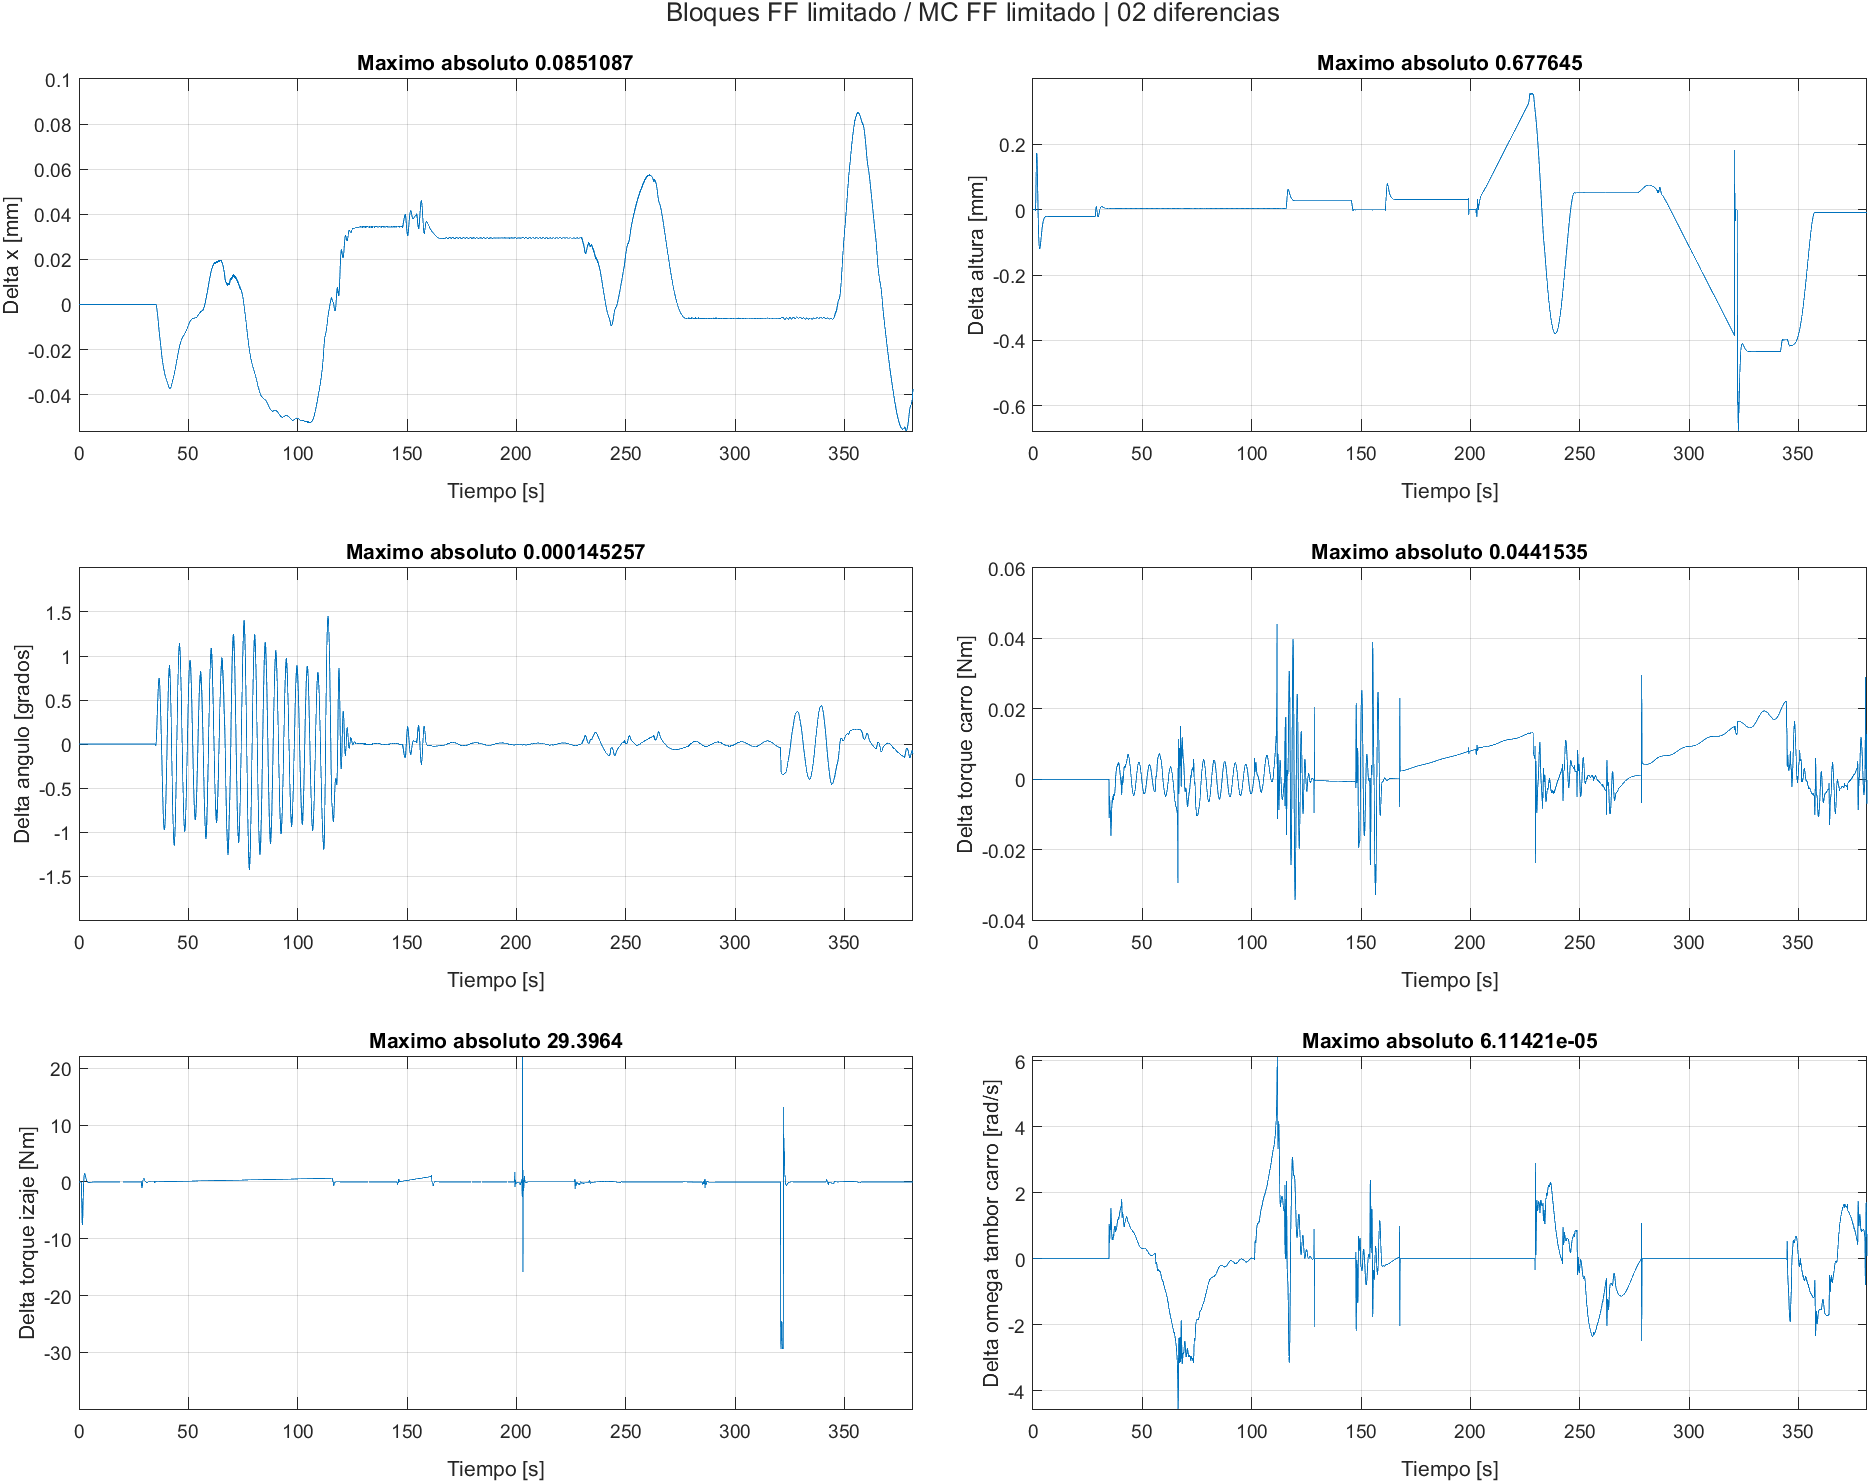
\includegraphics[width=15.0cm,height=6.05cm,keepaspectratio,trim=0.00bp 0.00bp 0.00bp 0.00bp,clip]{imagenes/r_061.png}}\par\note{La escala pequeña de las diferencias permite verificar la realización discreta.}
\end{frame}
\section{Pruebas completas MIL y SIL}
\begin{frame}[plain,label=seccion8]
\setbeamertemplate{frametitle}{}
\vfill
{\fontsize{25}{29}\selectfont\bfseries Validación completa: MIL y SIL\par}
\vspace{4mm}\textcolor{accent}{\rule{.75\linewidth}{1pt}}\par\vspace{3mm}
{\large Evaluación de la maniobra con planta, supervisor y control integrados.\par}\vfill
\note{Ubicar este bloque en el recorrido y anunciar su objetivo.}
\end{frame}
\begin{frame}[t,label=slide59]{Qué se verifica en cada banco}
\begin{center}
{\small\renewcommand{\arraystretch}{1.0}
\begin{tabular}{p{3.6cm}p{5.0cm}p{4.9cm}}\toprule
Prueba & Escenario & Objetivo\\\midrule
Completa MIL & 6 → 23; vacío → 32; 32 → 1 & Integración en Simulink\\
Medio ciclo SIL & 2 → 22, perfil precargado & SFC / ST y aporte anti-sway\\
Completa SIL & 6 → 23; vacío → 32; 32 → 1 & Integración con PLC\\
Productividad MIL & 2 → 22 → 2; retorno a 25 m & Requisito de ciclo cerrado\\
\bottomrule\end{tabular}}\end{center}
Cada tiempo se interpreta con sus fronteras, operador y condiciones de ensayo.
\note{Esta tabla evita extrapolar un resultado entre escenarios. La prueba completa comprueba funcionamiento; la productividad requiere además un retorno vacío al inicio.}
\end{frame}
\begin{frame}[t,label=slide60]{Prueba completa MIL: escena y transferencias}
\begin{center}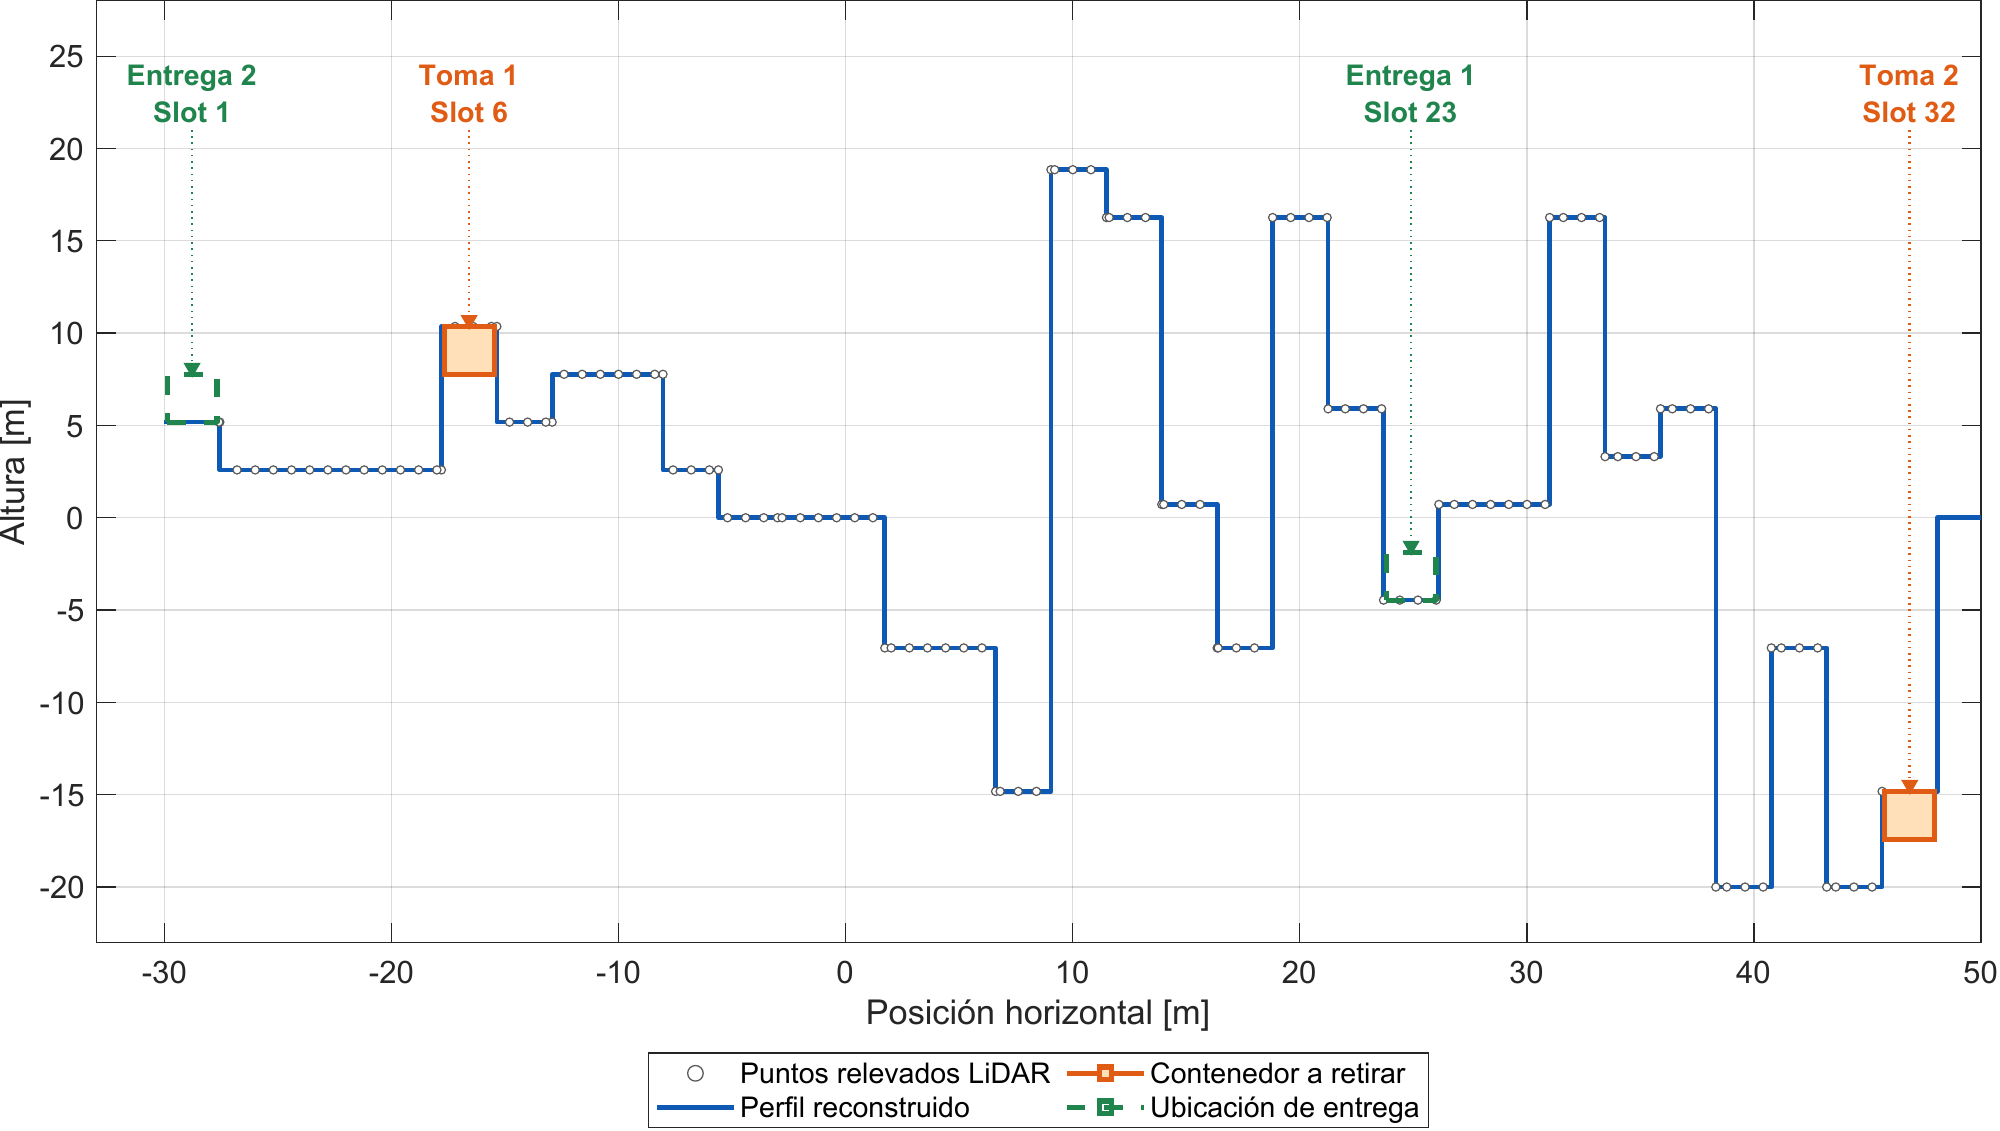
\includegraphics[width=.98\linewidth,height=5.55cm,keepaspectratio]{imagenes/r_063.png}\end{center}\vspace{-1mm}\figcaption{Barrido real; dos tomas y dos entregas en sentidos opuestos.}
\note{Describir 6→23, reposicionamiento vacío al32 y 32→1. Se actualiza el perfil en cada toma y entrega; no hay retorno vacío final.}
\end{frame}
\begin{frame}[t,label=slide61]{Prueba completa MIL: movimiento del carro}
\relax
\figurefooter{Posición, velocidad y aceleración reconstruidas desde el accionamiento.}
\vspace{-2mm}\makebox[\linewidth][c]{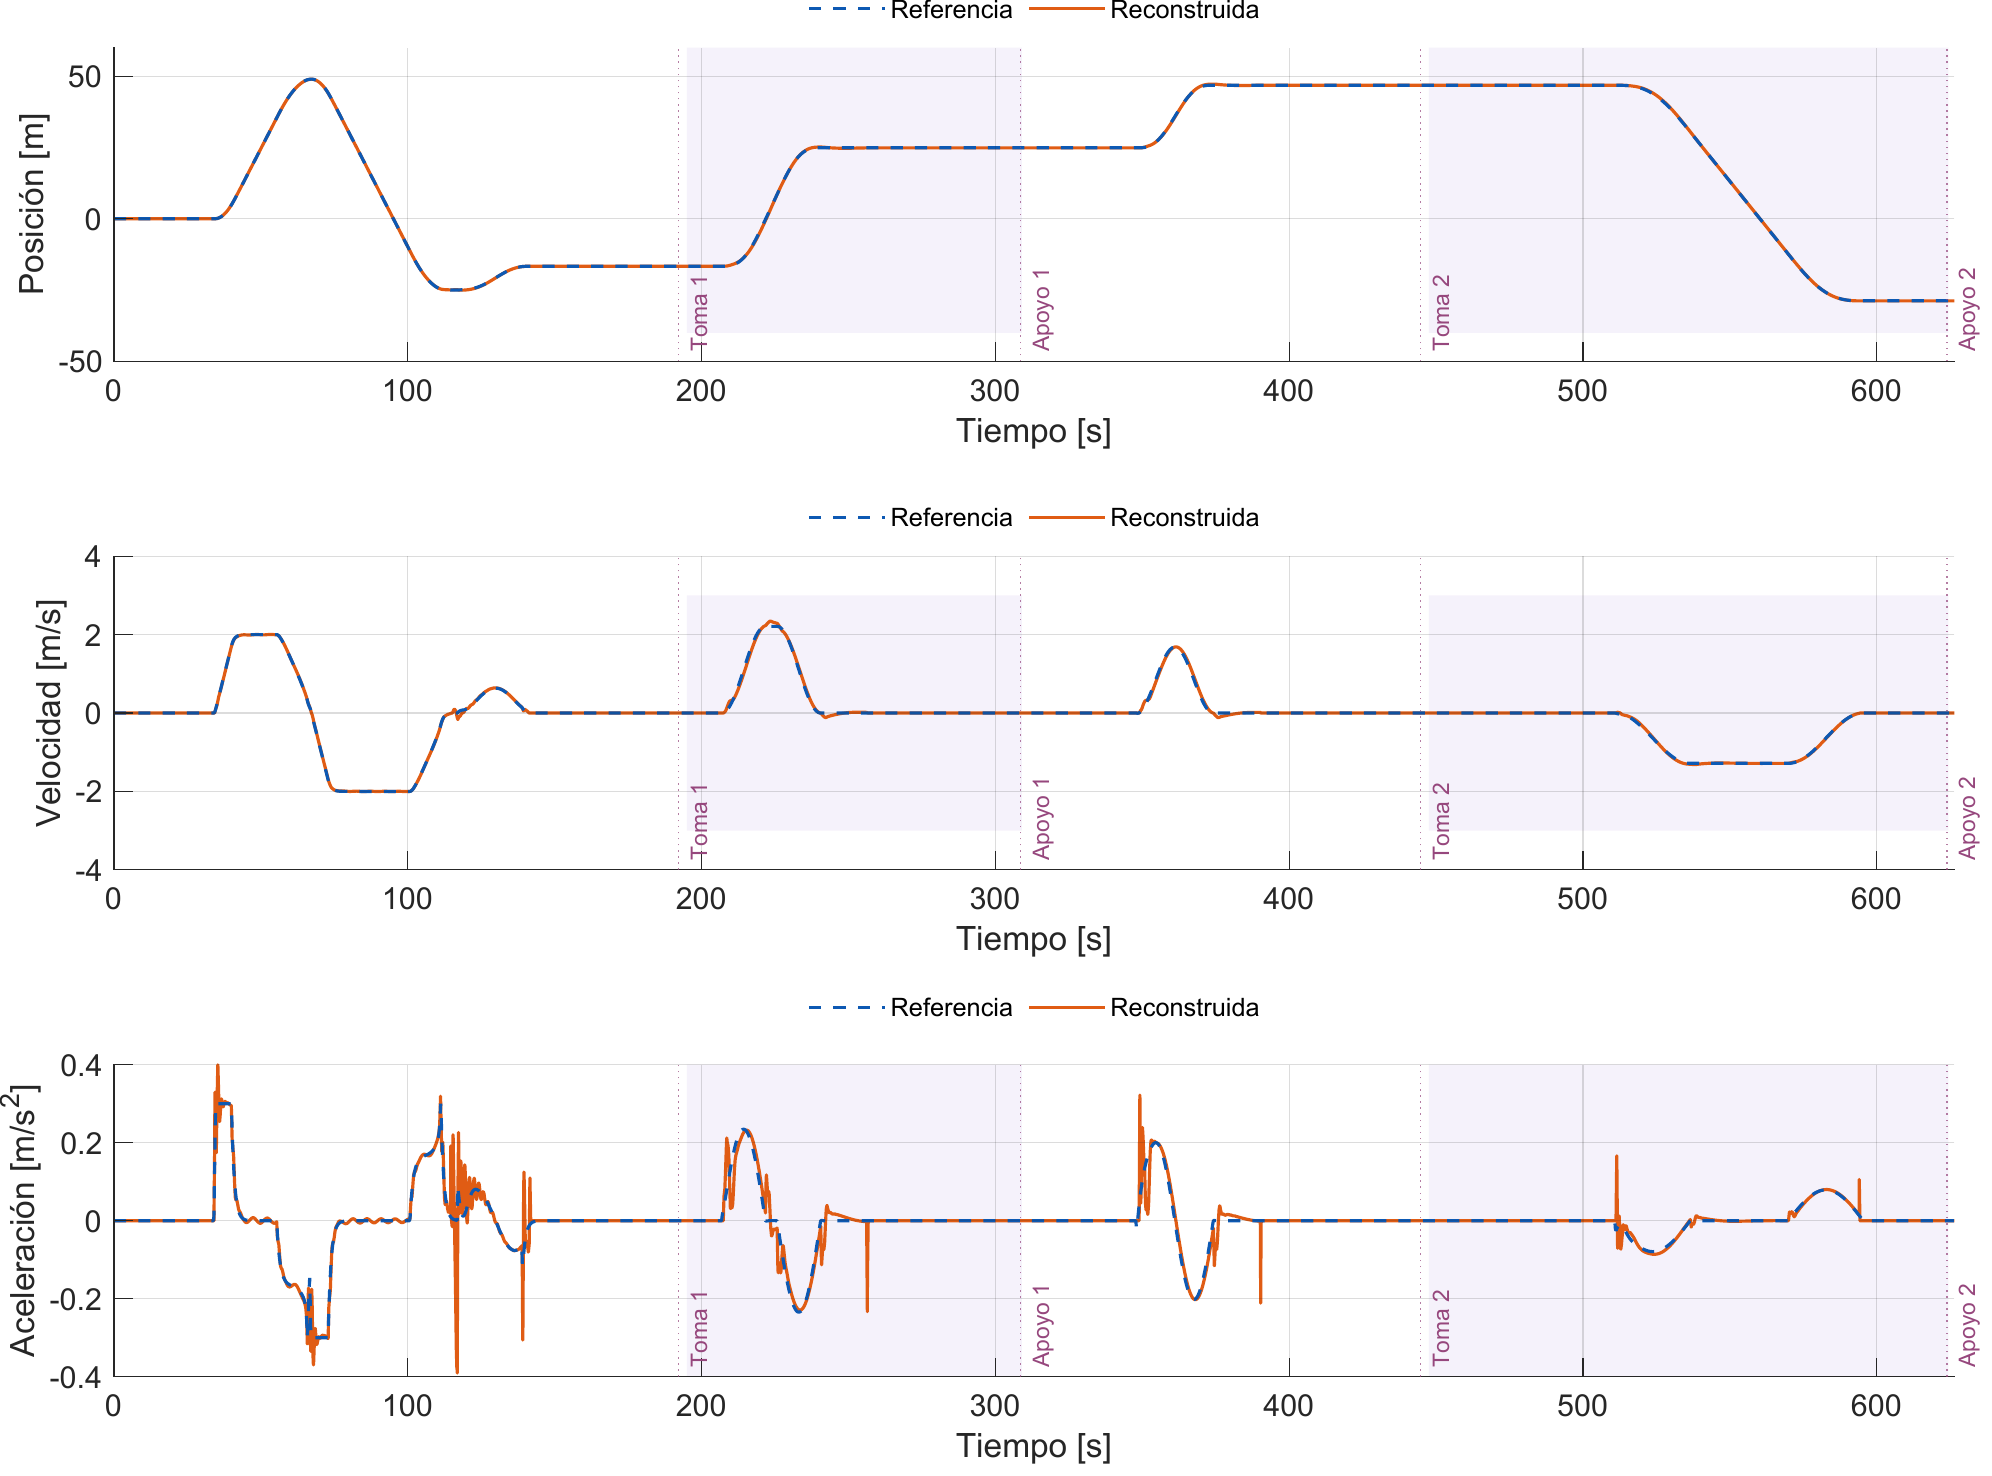
\includegraphics[width=15.0cm,height=6.05cm,keepaspectratio,trim=0.00bp 7.00bp 7.00bp 0.00bp,clip]{imagenes/r_065.png}}\par\note{Las franjas muestran las transferencias cargadas. Leer referencias y medidas; la aceleración reconstruida no es la aceleración física del carro.}
\end{frame}
\begin{frame}[t,label=slide62]{Prueba completa MIL: movimiento de izaje}
\relax
\figurefooter{Altura inferida del accionamiento y sus derivadas frente a referencias.}
\vspace{-2mm}\makebox[\linewidth][c]{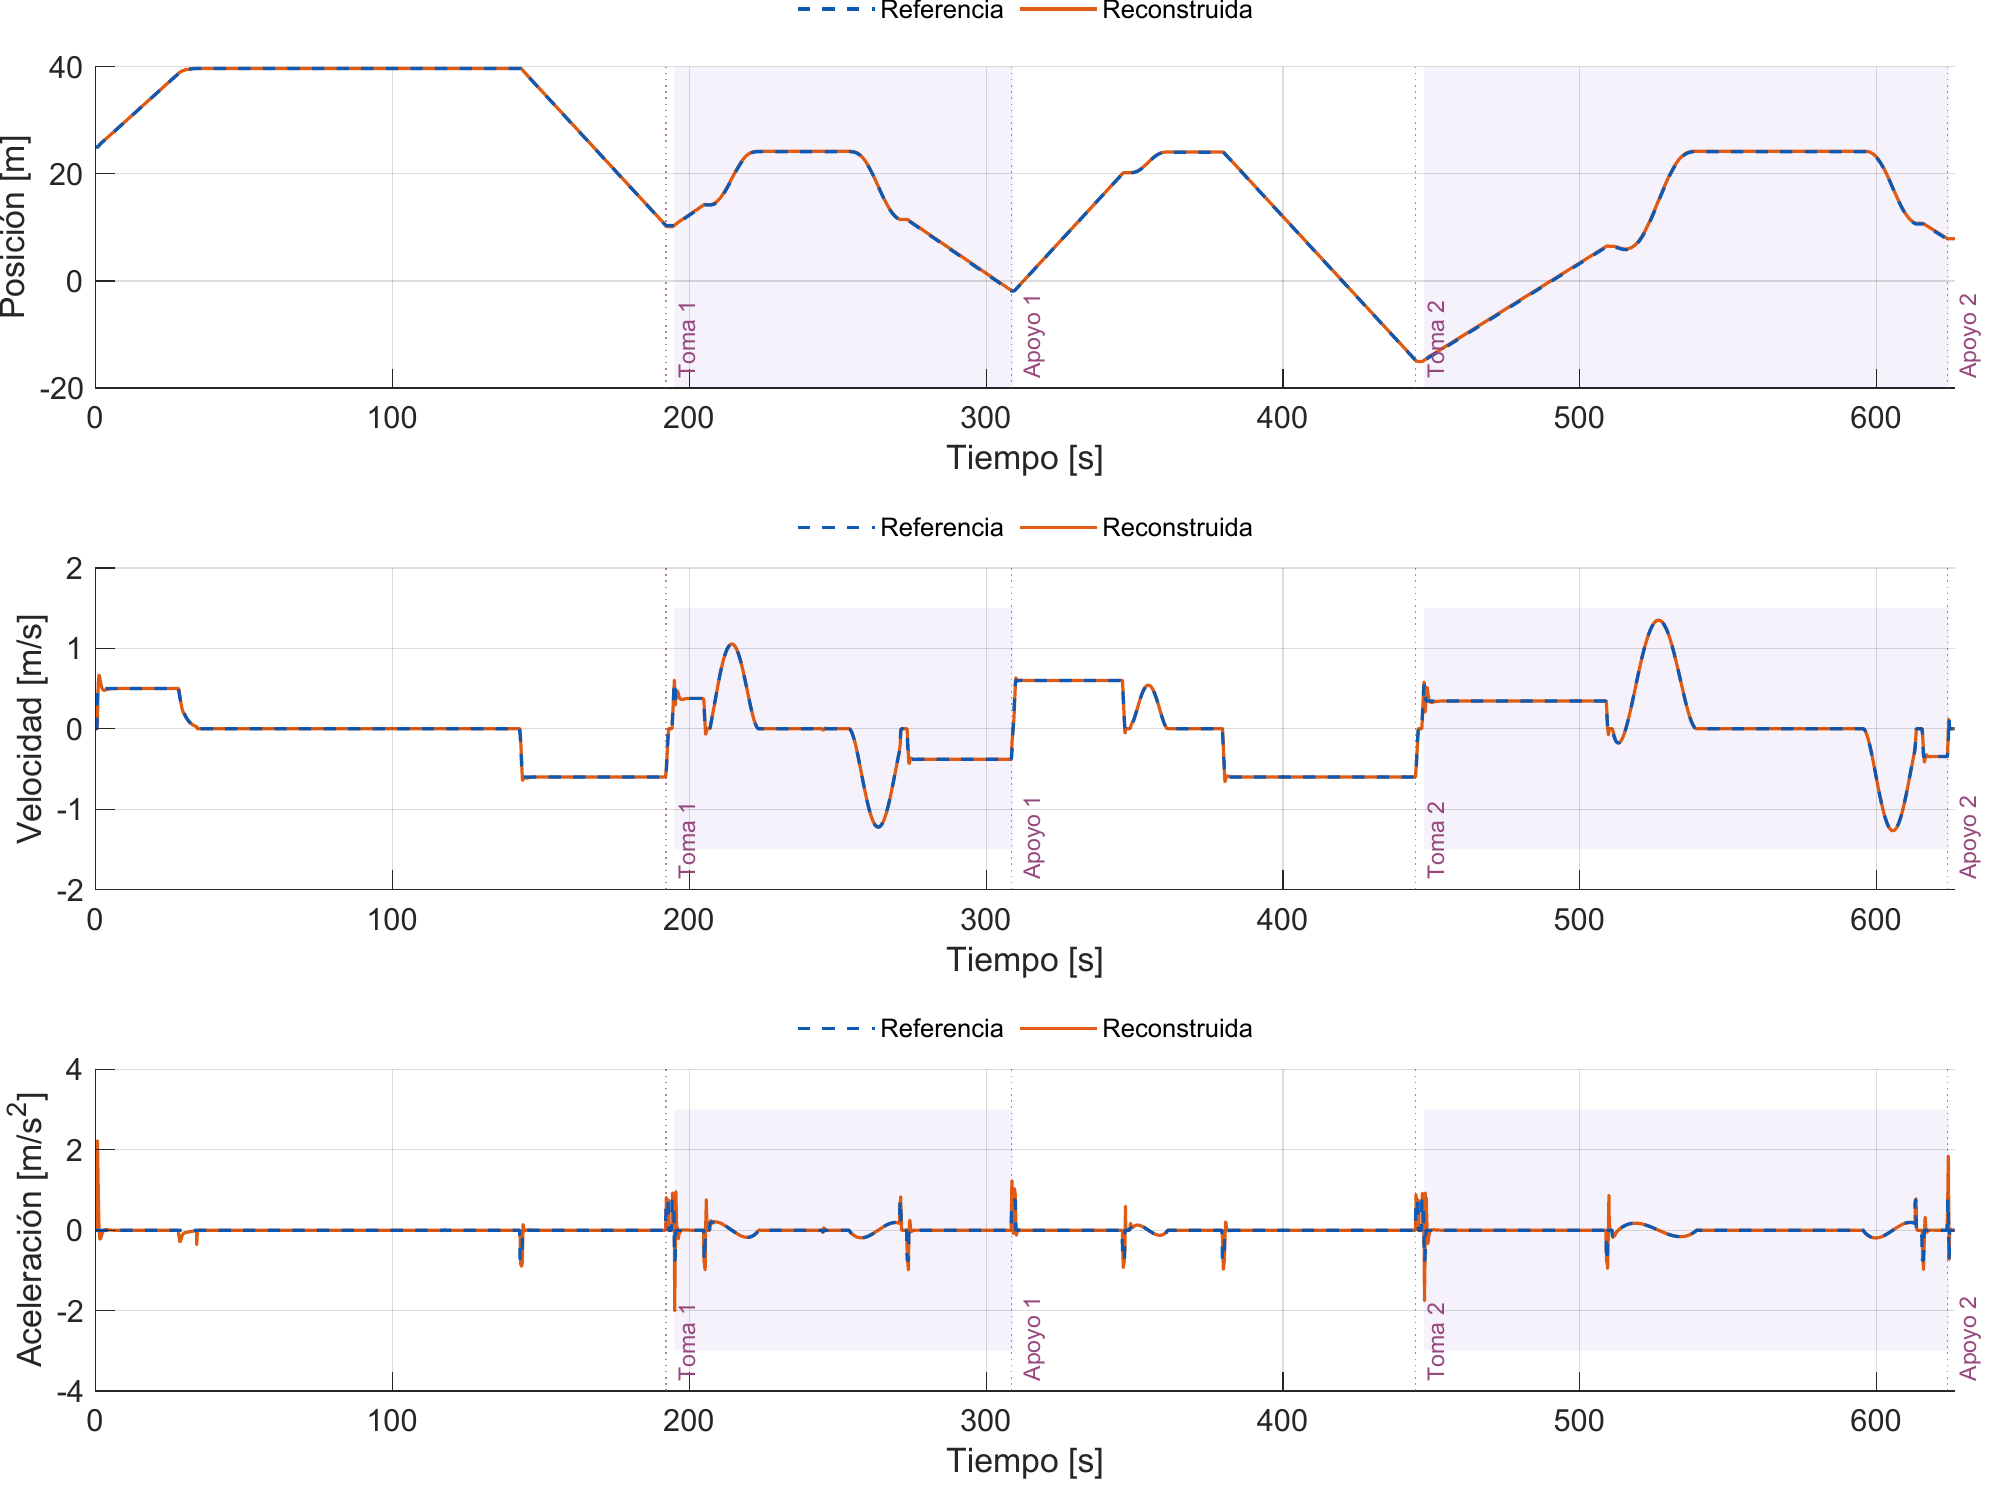
\includegraphics[width=15.0cm,height=6.05cm,keepaspectratio,trim=0.00bp 7.00bp 7.00bp 0.00bp,clip]{imagenes/r_066.png}}\par\note{Relacionar los niveles con barrido, toma y entrega. Los impactos de la carga física no deben leerse a partir de esta aceleración de accionamiento.}
\end{frame}
\begin{frame}[t,label=slide63]{Prueba completa MIL: balanceo}
\relax
\figurefooter{El barrido y las maniobras posteriores se presentan con escalas distintas.}
\vspace{-2mm}\makebox[\linewidth][c]{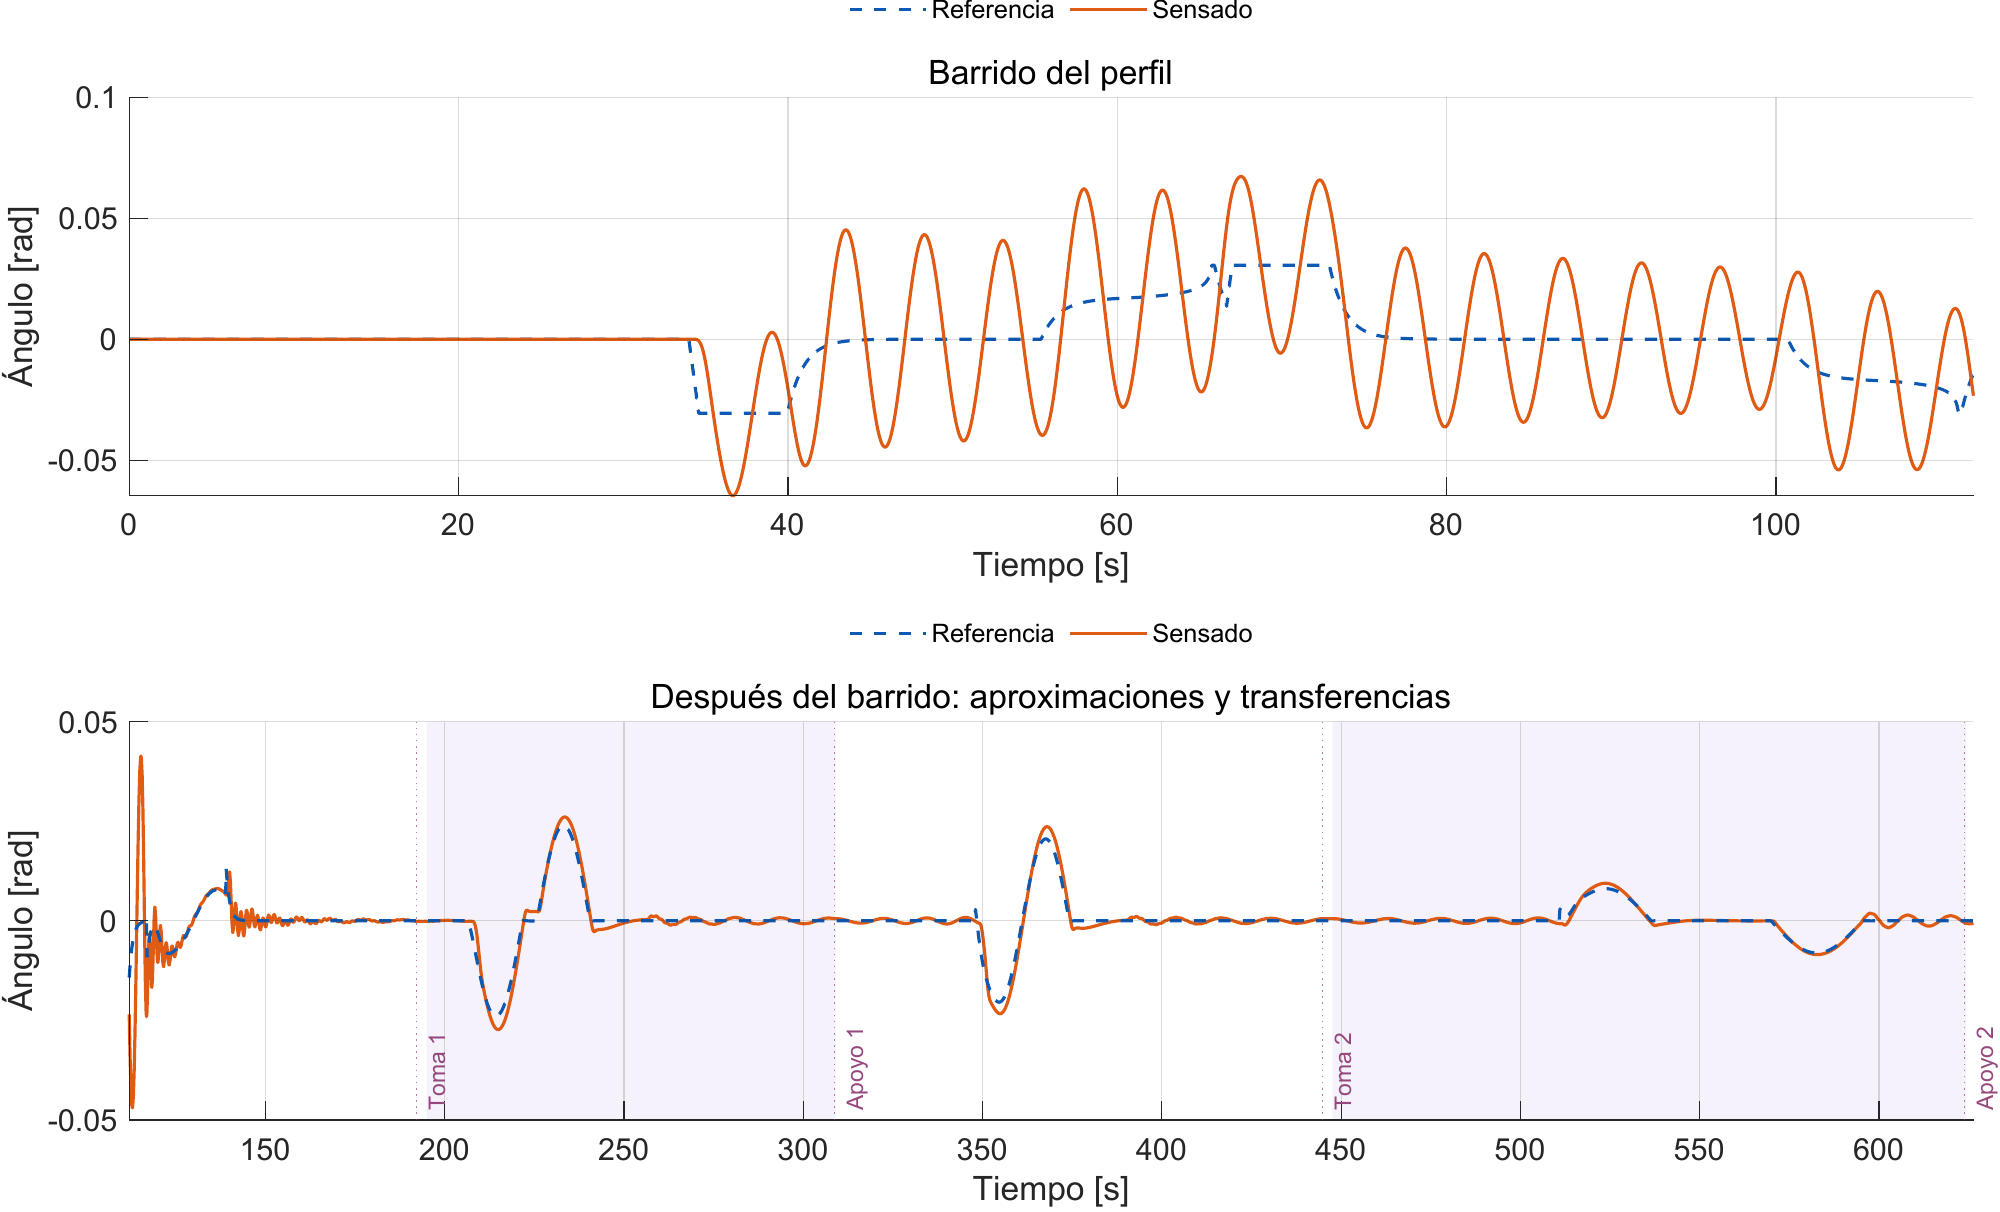
\includegraphics[width=15.0cm,height=6.05cm,keepaspectratio,trim=0.00bp 0.00bp 0.00bp 0.00bp,clip]{imagenes/r_067.png}}\par\note{Mostrar la evolución angular y la referencia durante cada traslado. Maximos en AUTO: 0,0273 y 0,0094 rad; las maniobras manuales tienen condiciones distintas.}
\end{frame}
\begin{frame}[t,label=slide64]{Prueba completa MIL: resumen}
\begin{center}
{\small\renewcommand{\arraystretch}{1.0}
\begin{tabular}{lr}\toprule
Etapa & Duración [s]\\\midrule
Primera toma → entrega en barco & 114,04\\
AUTO cargado hacia barco & 63,96\\
Entrega → segunda toma & 138,56\\
Segunda toma → entrega en muelle & 176,76\\
AUTO cargado hacia muelle & 101,92\\
\bottomrule\end{tabular}}\end{center}
\begin{itemize}
\item Parada normal a 626,36 s; dos tomas y dos entregas físicas.
\item Balance correcto del perfil y conjunto vacío al final.
\item Sin emergencias ni fallas de seguimiento desde START.
\item Torque máximo: 1,073 kN m en carro y 15,294 kN m en izaje.
\end{itemize}
\note{Las filas AUTO están contenidas en las transferencias; no se suman nuevamente. Los tiempos no son un ciclo simple comparable con 120 s.}
\end{frame}
\begin{frame}[t,label=slide65]{Medio ciclo SIL: condiciones comunes}
\begin{itemize}
\item Slot 2 → 22: 48,80 m; inicio en x = −26,34 m y altura 25 m.
\item Contenedor: 36 863 kg; conjunto cargado: 51 863 kg.
\item Perfil físico de 33 alturas, precargado; máximo 18,85 m.
\item Misma planta, MC, ganancias y operador para SFC y ST.
\item Tercera prueba: SFC manual con anti-sway desactivado.
\end{itemize}
\note{Explicar que se parte con perfil válido y sin barrido. El banco sincroniza las tramas a tiempo simulado; se preservan los tiempos originales de cada corrida.}
\end{frame}
\begin{frame}[t,label=slide66]{Medio ciclo SIL: seguimiento y eventos SFC/ST}
\relax
\figurefooter{Cada ejecución conserva sus referencias y tiempos.}
\begin{columns}[T,onlytextwidth]
\column{.68\textwidth}
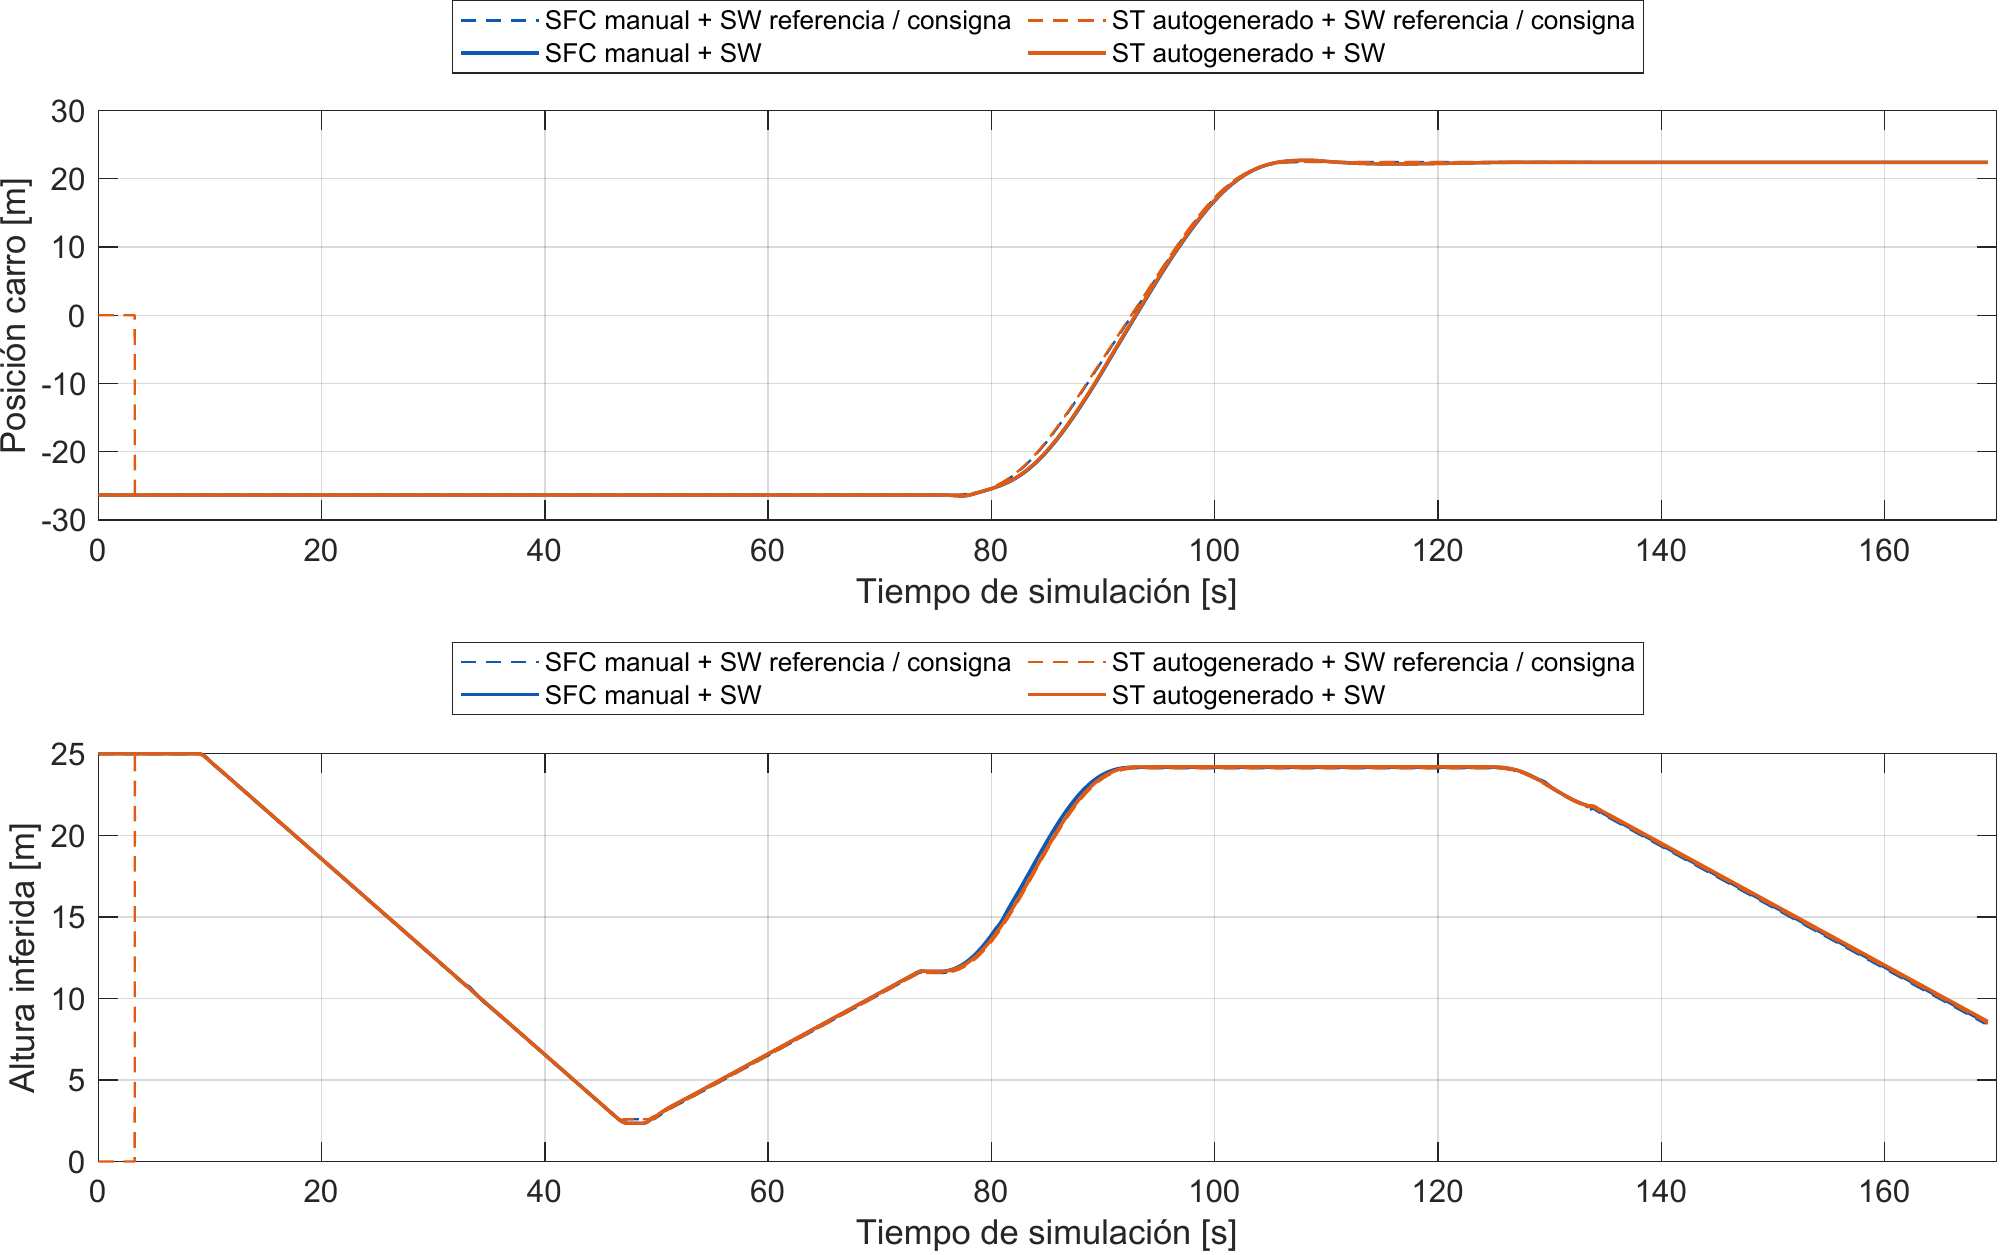
\includegraphics[width=\linewidth,height=5.8cm,keepaspectratio]{imagenes/r_086.png}\par

\column{.30\textwidth}\vspace{5mm}
\fontsize{8}{9.6}\selectfont
\begin{tabular}{lrr}\toprule
Evento & SFC [s] & ST [s]\\\midrule
START & 3,24 & 3,24\\
Toma & 49,56 & 49,52\\
Entrada AUTO & 75,44 & 75,40\\
Llegada $x$ & 105,84 & 105,76\\
Manual destino & 133,32 & 133,56\\
Apoyo destino & 168,92 & 169,24\\\bottomrule
\end{tabular}\par\vspace{4mm}
\figcaption{Ambas implementaciones alcanzaron el apoyo y permitieron actuar sobre los twistlocks.}
\end{columns}
\note{Las curvas se superponen en buena parte del recorrido. No desplazar curvas para hacer coincidir eventos; mostrar la semejanza y los pequeños desfasajes. Concluir equivalencia funcional en el escenario ensayado, sin afirmar identidad de todas las guardas de seguridad. Los registros mostrados terminan en parada o apoyo según corrida.}
\end{frame}
\begin{frame}[t,label=slide68]{Medio ciclo SIL: balanceo con y sin anti-sway}
\relax
\figurefooter{Con y sin anti-sway; umbrales angulares de habilitación del descenso.}
\vspace{-2mm}\makebox[\linewidth][c]{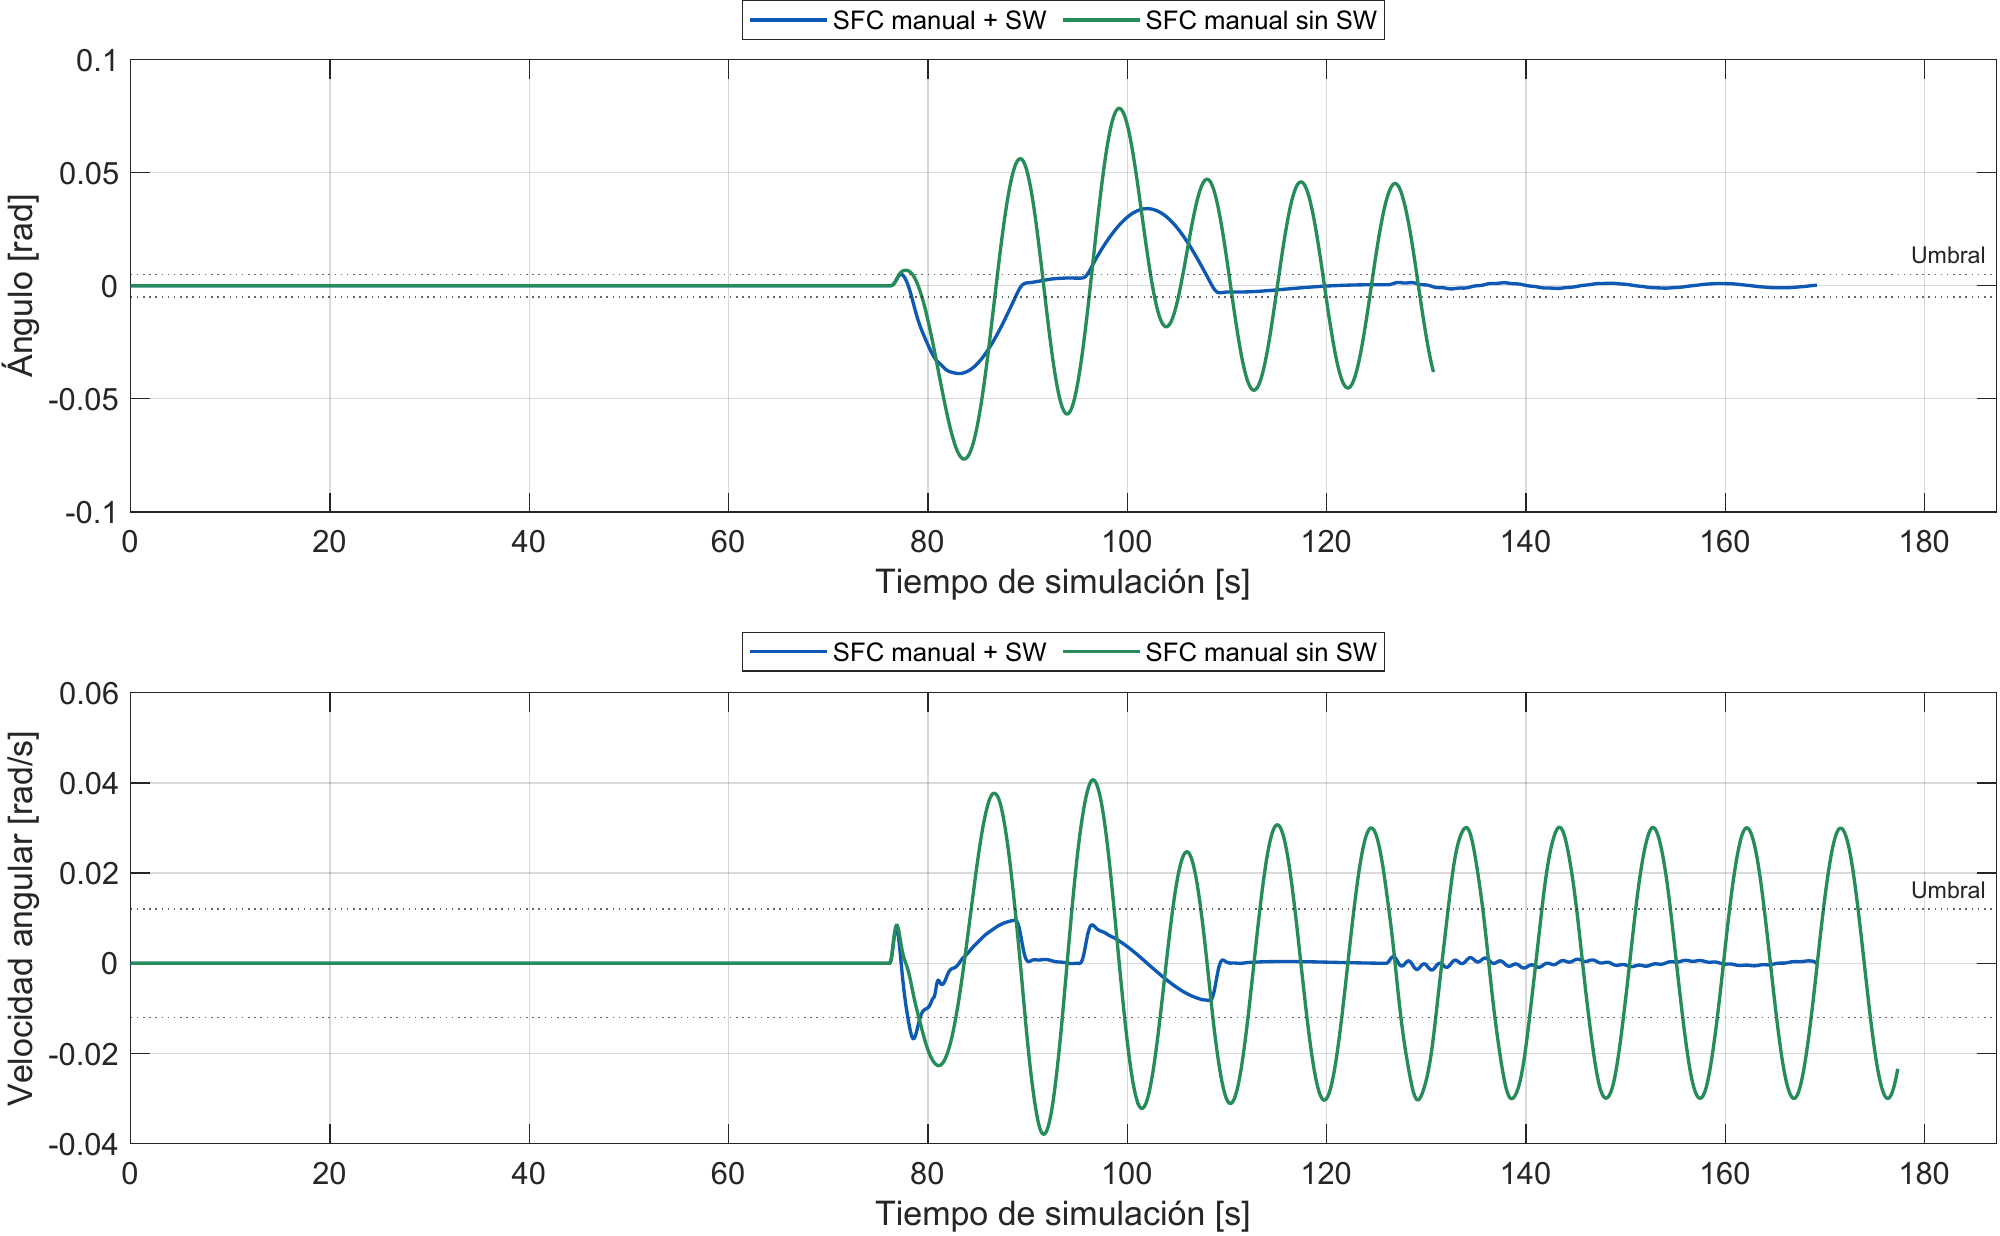
\includegraphics[width=15.0cm,height=6.05cm,keepaspectratio,trim=0.00bp 0.00bp 0.00bp 0.00bp,clip]{imagenes/r_092.png}}\par\note{Sin corrección llega el carro pero persiste el balanceo. La prueba termina a 187,20 s con el contenedor suspendido y sin entrega.}
\end{frame}
\begin{frame}[t,label=comparacionantisway]{Medio ciclo SIL: resultado de activar el anti-sway}
\begin{center}\small
\begin{tabular}{lrr}\toprule
Ventana común 120--130,72 s & Con anti-sway & Sin anti-sway\\\midrule
Ángulo RMS [$^\circ$] & 0,0395 & 1,789\\
Ángulo máximo [$^\circ$] & 0,0826 & 2,590\\
Velocidad angular RMS [$^\circ$/s] & 0,0330 & 1,244\\\bottomrule
\end{tabular}\end{center}
\begin{itemize}
\item Con anti-sway se satisfacen las guardas de balanceo y continúa el descenso hacia la entrega.
\item Sin anti-sway el carro llega, pero queda inhibido el descenso. El ensayo termina a 187,20 s con la carga suspendida.
\item La reducción angular RMS es 97,8\,\% en esta ventana y configuración.
\end{itemize}
\note{Conversión radianes a grados de las métricas del informe. Misma planta, MC, ganancias y operador. No convertir este porcentaje en una mejora universal de todos los ciclos.}
\end{frame}

\begin{frame}[t,label=slide70]{Prueba completa SIL: seguimiento horizontal}
\relax
\figurefooter{Autómatas SFC manuales; barrido y dos transferencias; sincronización de tramas de 20 ms.}
\vspace{-2mm}\makebox[\linewidth][c]{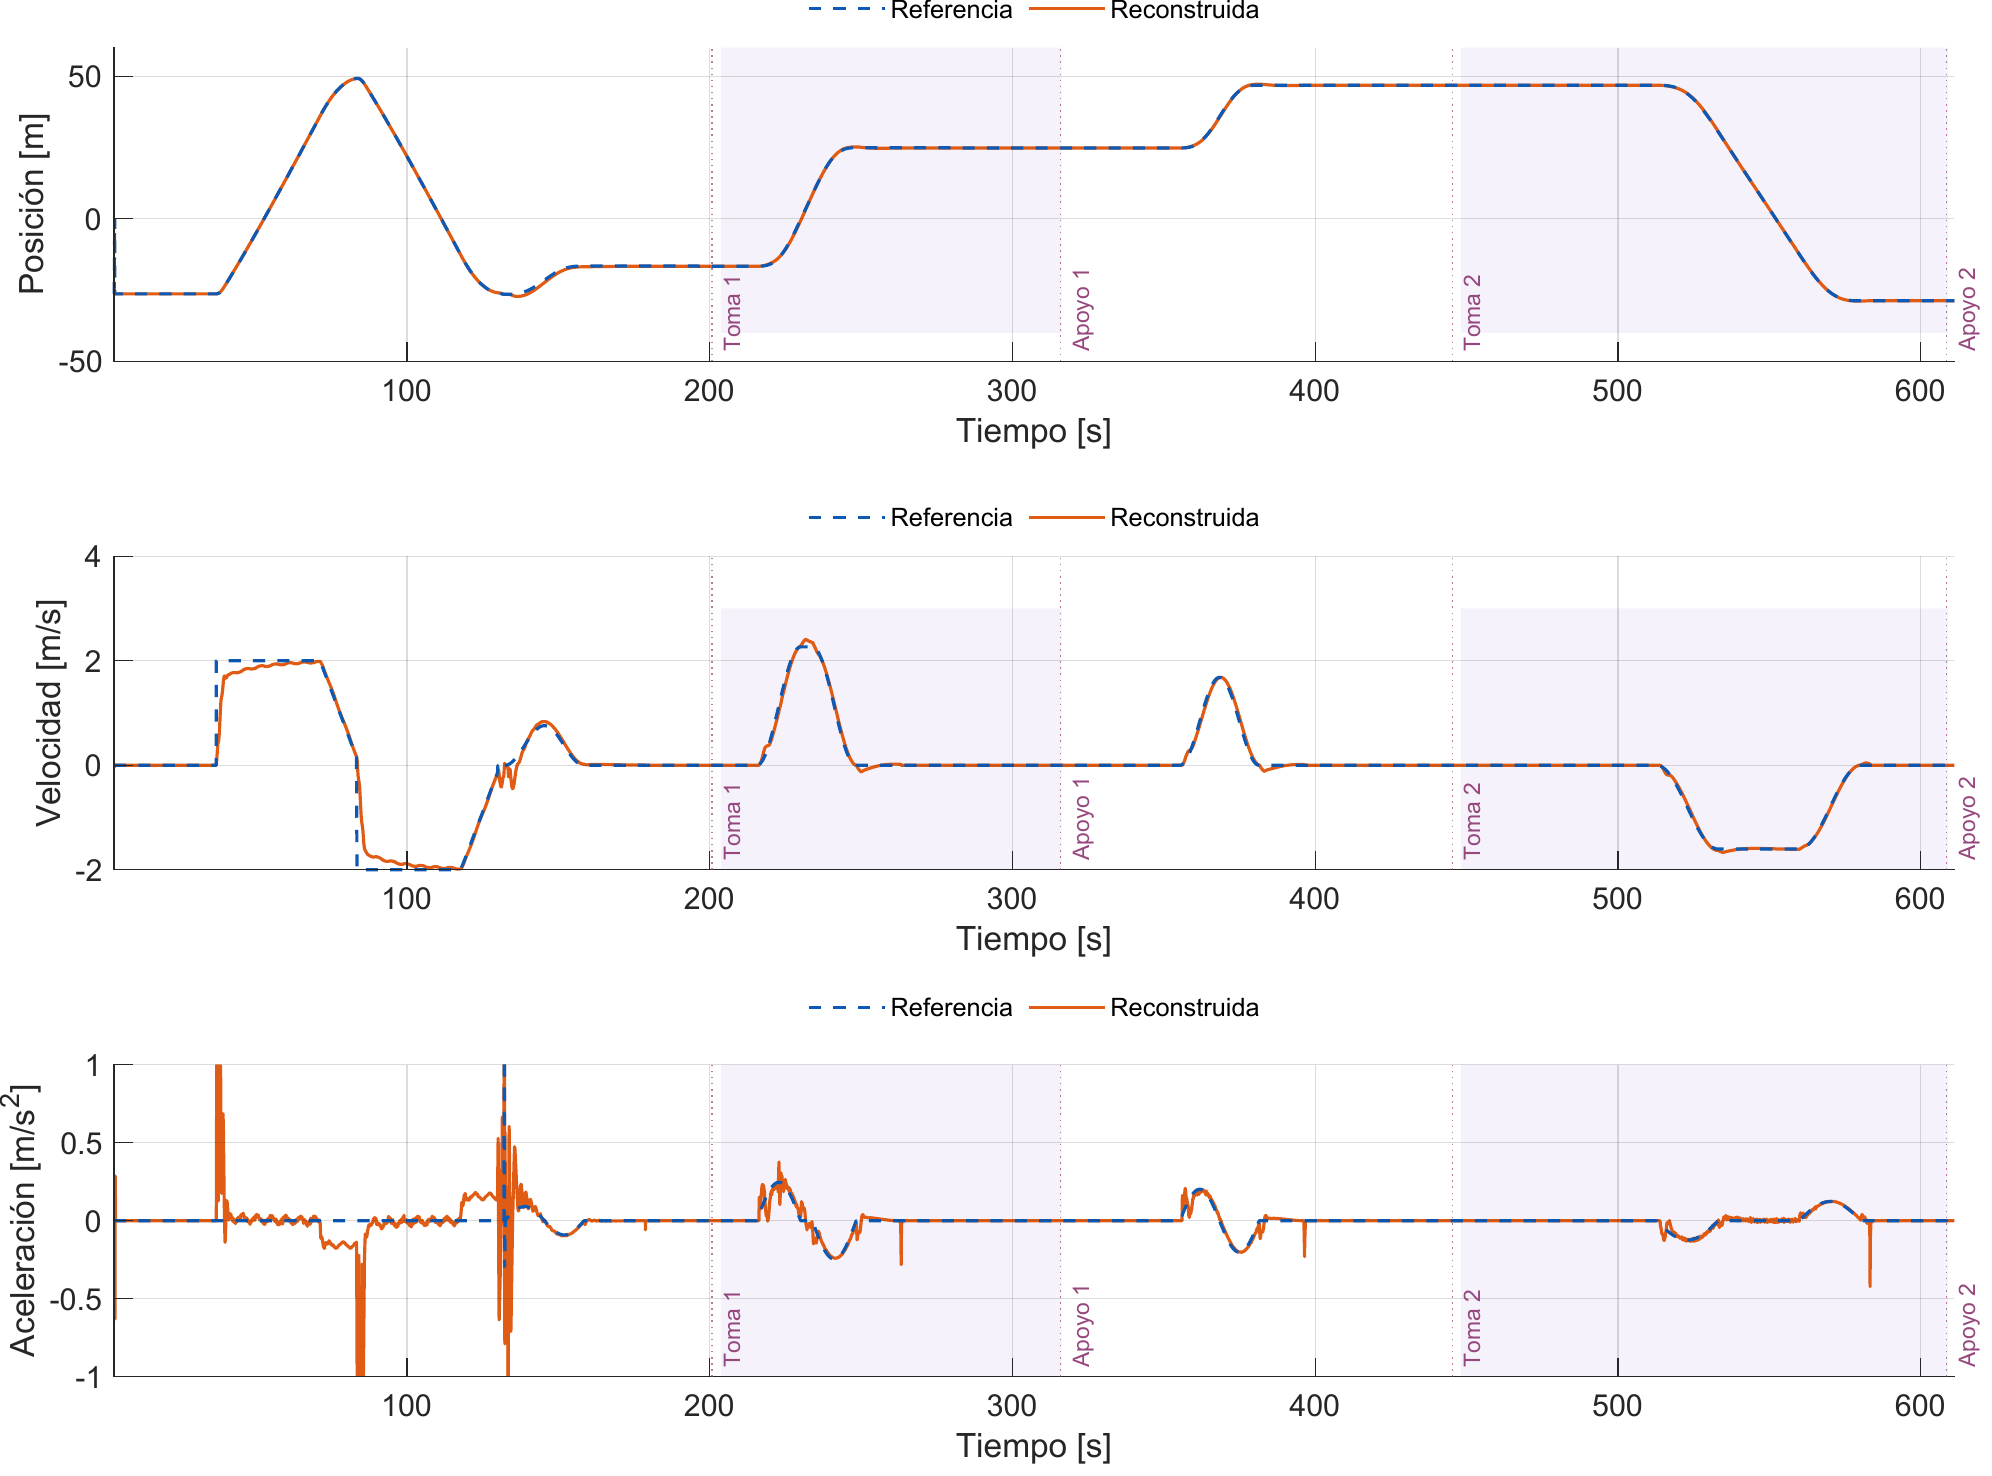
\includegraphics[width=15.0cm,height=6.05cm,keepaspectratio,trim=0.00bp 7.00bp 7.00bp 0.00bp,clip]{imagenes/r_074.png}}\par\note{El banco utiliza OPC UA con SignAndEncrypt. Explicar que la telemetría del operador registra eventos cada 40 ms; la tasa de tarea es20 ms.}
\end{frame}
\begin{frame}[t,label=slide71]{Prueba completa SIL: izaje}
\relax
\figurefooter{Magnitudes reconstruidas del accionamiento; aceleración mostrada entre ±1 m/s$^2$.}
\vspace{-2mm}\makebox[\linewidth][c]{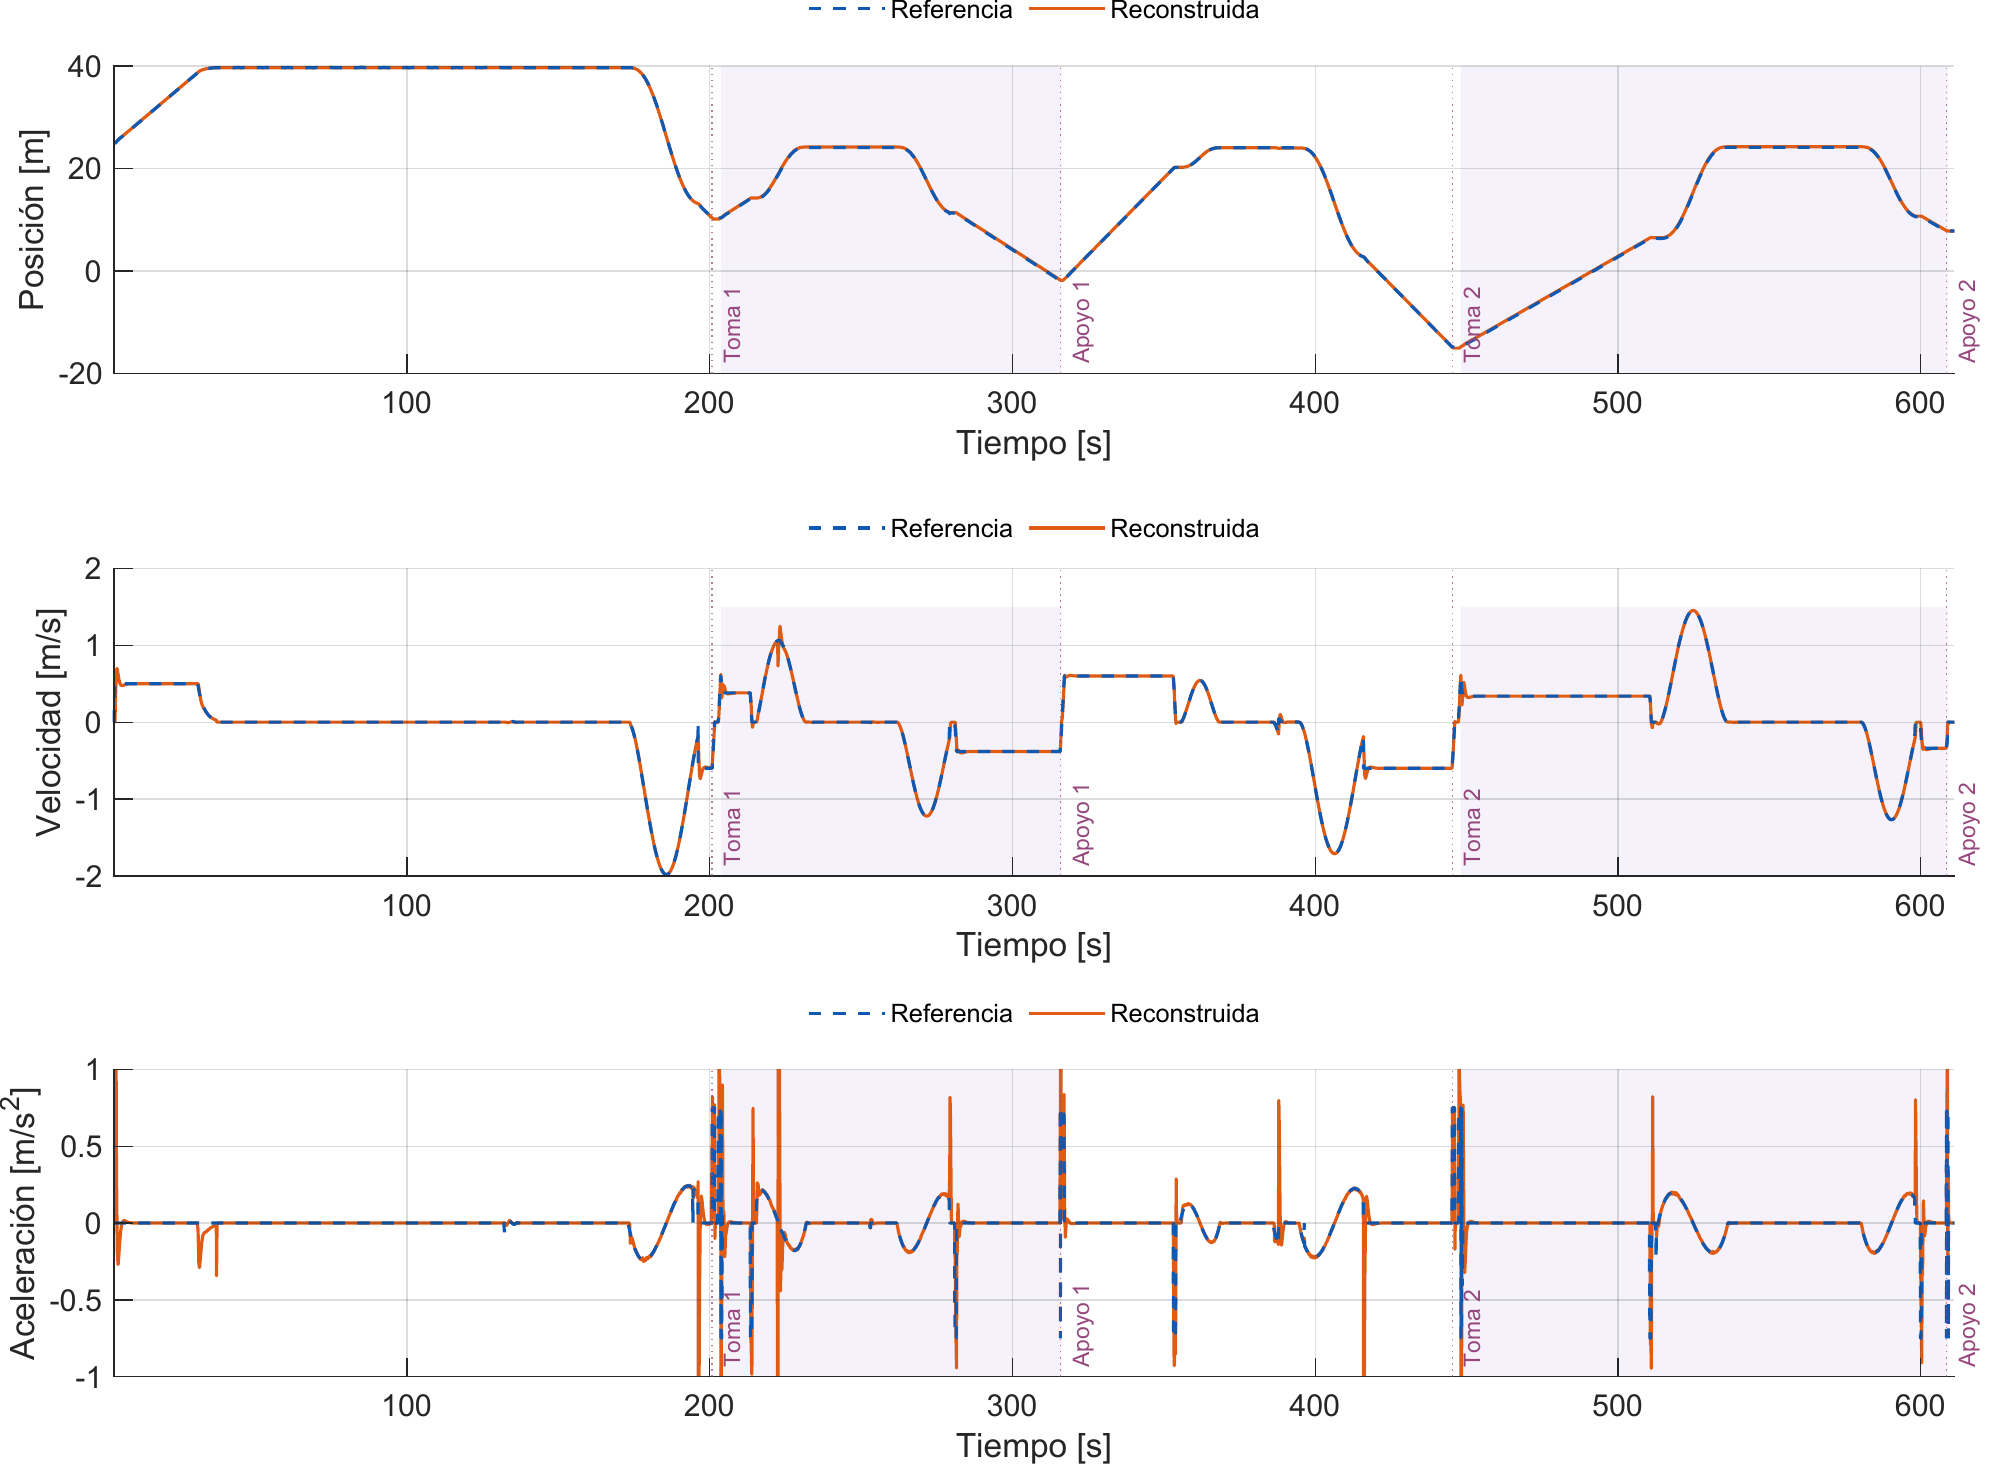
\includegraphics[width=15.0cm,height=6.05cm,keepaspectratio,trim=0.00bp 7.00bp 7.00bp 0.00bp,clip]{imagenes/r_075.png}}\par\note{Advertir al explicar la gráfica que la escala recorta picos: no representa ausencia de transitorios. El contacto físico vertical genera otros picos, de naturaleza diferente.}
\end{frame}
\begin{frame}[t,label=slide72]{Prueba completa SIL: balanceo y esfuerzo}
\relax
\figurefooter{Ángulo medido y de referencia; escalas separadas para barrido y maniobras.}
\vspace{-2mm}\makebox[\linewidth][c]{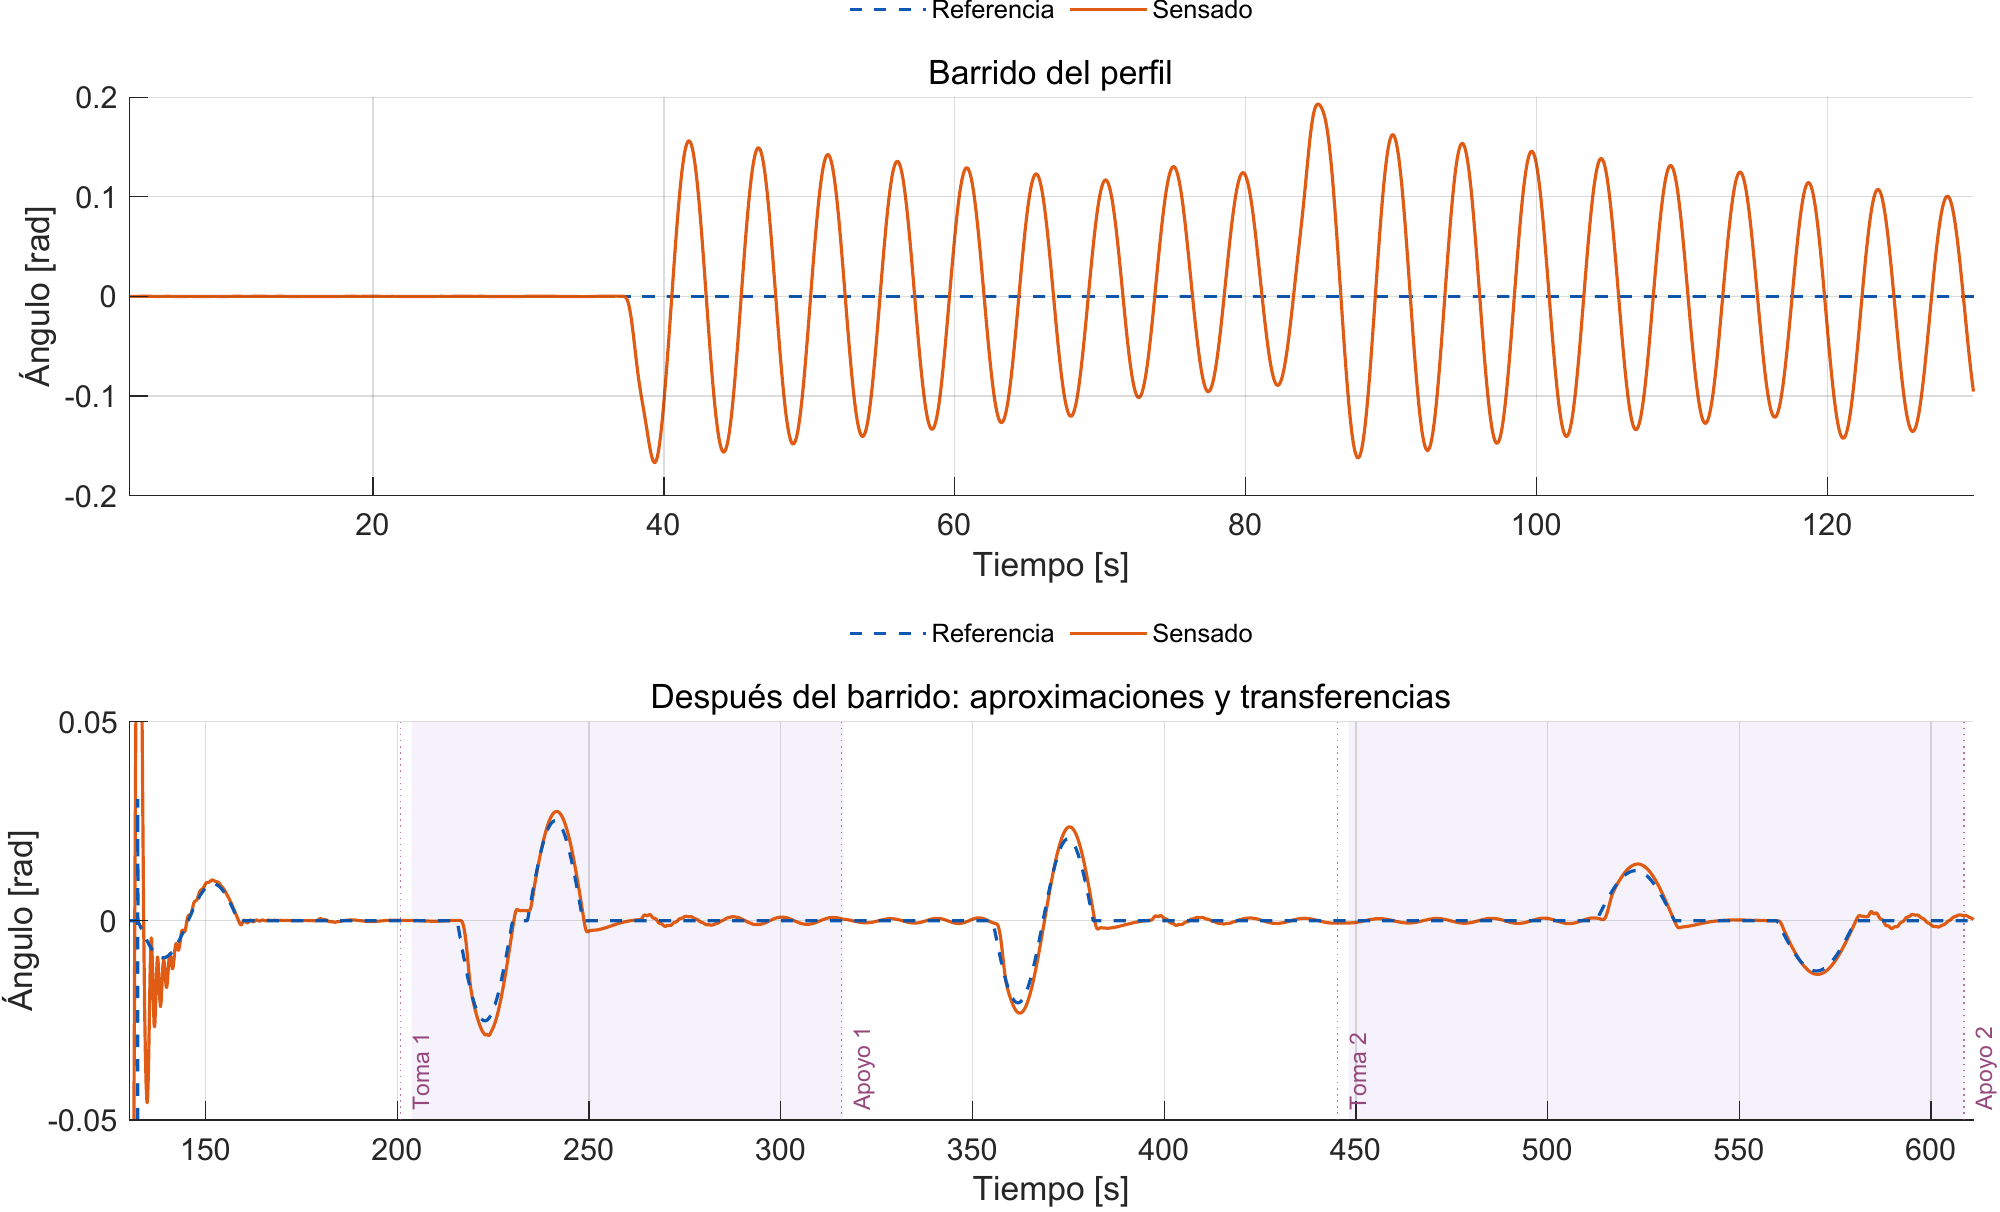
\includegraphics[width=15.0cm,height=6.05cm,keepaspectratio,trim=0.00bp 0.00bp 0.00bp 0.00bp,clip]{imagenes/r_076.png}}\par\note{Maximos AUTO: 0,02877 y 0,01425 rad. Los torques máximos fueron1,699 y15,212kNm; si se pregunta mostrar gráfica de torques en respaldo.}
\end{frame}
\begin{frame}[t,label=slide73]{Prueba completa SIL: resultados}
\begin{center}
{\small\renewcommand{\arraystretch}{1.0}
\begin{tabular}{lr}\toprule
Etapa & Duración [s]\\\midrule
Primera toma → entrega en barco & 112,56\\
AUTO cargado hacia barco & 63,28\\
Entrega → segunda toma & 131,88\\
Segunda toma → entrega en muelle & 160,92\\
AUTO cargado hacia muelle & 85,08\\
\bottomrule\end{tabular}}\end{center}
\begin{itemize}
\item Dos tomas y entregas; masa y perfiles finales coherentes.
\item Parada normal a 611,08 s; sin retorno vacío final.
\item Sin fallas ni emergencias desde START.
\item Los tiempos MIL/SIL no comparan directamente productividad.
\end{itemize}
\note{El desempeño temporal depende de operador, recorrido y sincronización. La primera transferencia de112,56s no incluye el regreso al origen; evitar usar3600/112,56como productividad del ciclo.}
\end{frame}
\section{Estimación y mejora de productividad}
\begin{frame}[plain,label=seccion9]
\setbeamertemplate{frametitle}{}
\vfill
{\fontsize{25}{29}\selectfont\bfseries Productividad y optimización\par}
\vspace{4mm}\textcolor{accent}{\rule{.75\linewidth}{1pt}}\par\vspace{3mm}
{\large Tiempo de ciclo, ajuste de la trayectoria y verificación de resultados.\par}\vfill
\note{Ubicar este bloque en el recorrido y anunciar su objetivo.}
\end{frame}
\begin{frame}[t,label=slide74]{Definir un ciclo para evaluar productividad}
\begin{itemize}
\item Inicio: spreader vacío sobre slot 2, x = −26,34 m, altura 25 m.
\item Perfil conocido; mismo contenedor de 36 863 kg.
\item Descenso, toma, pesaje, traslado al slot 22 y entrega.
\item Retorno vacío al slot 2 y a la altura inicial.
\item Cronometraje: desde inicio del descenso hasta confirmar reposo.
\end{itemize}\[
P=\frac{3600}{T_{ciclo}},\qquad P_{req}=30\ \mathrm{h^{-1}}\Rightarrow T_{req}=120\ \mathrm{s}
\]

\note{Introducir un único escenario, evaluar primero el MC FF y recién después plantear la mejora. El barrido inicial y las demoras logísticas quedan fuera de este ensayo.}
\end{frame}
\begin{frame}[t,label=slide75]{Condición de regreso y cierre del ciclo}
\begin{center}
{\small\renewcommand{\arraystretch}{1.0}
\begin{tabular}{p{4.5cm}p{9.1cm}}\toprule
Variable & Criterio de confirmación\\\midrule
Conjunto suspendido & Spreader vacío\\
Posición horizontal & Error $\leq0,08$ m\\
Altura & $25\pm0,10$ m\\
Velocidades & $|v_x|<0,06$; $|v_y|<0,08$ m/s\\
Balanceo & $|\theta|\leq0,5^\circ$; $|\omega|\leq0,05$ rad/s\\
Permanencia & 0,20 s\\
\bottomrule\end{tabular}}\end{center}

\note{La condición de cierre se mantiene en la repetición ajustada. Es fundamental que el regreso no sea solamente llegar a la coordenada horizontal.}
\end{frame}
\begin{frame}[t,label=slide76]{Prueba de ciclo cerrado inicial: Motion Controller FF}
\[
T_0=219{,}92-2{,}00=217{,}92\ \mathrm{s}
\]
\[
P_0=\frac{3600}{217{,}92}=16{,}52\ \mathrm{contenedores/h}
\]
\begin{itemize}
\item Configuración FF de las pruebas previas.
\item Mandos manuales y esperas de 2 s antes de solicitar AUTO.
\item El ciclo excede el objetivo en 97,92 s.
\end{itemize}\vspace{2mm}\textcolor{accent}{\textbf{Se requiere reducir el tiempo inicial al menos un 44,93 \%.}}
\note{No anticipar la configuración corregida antes de establecer la necesidad. El resultado es problemático aunque las transferencias funcionales anteriores hayan sido exitosas.}
\end{frame}
\begin{frame}[t,label=slide77]{Prueba de ciclo cerrado inicial: tiempos por etapa}
\begin{center}
{\small\renewcommand{\arraystretch}{1.0}
\begin{tabular}{lr}\toprule
Etapa & Tiempo [s]\\\midrule
Descenso vacío hasta contacto & 37,72\\
Cierre de twistlocks & 1,04\\
Extracción, pesaje y solicitud AUTO & 23,88\\
AUTO cargado hasta solicitud MANUAL & 55,76\\
Manual, descenso y entrega & 30,72\\
Extracción vacía y solicitud AUTO & 22,00\\
AUTO vacío hasta regreso & 46,52\\
Confirmación de reposo & 0,28\\
\bottomrule\end{tabular}}\end{center}
\textbf{Traslados automáticos:} 102,28 s. \quad\textbf{Resto de maniobras:} 115,64 s.
\note{La tabla contiene ocho etapas consecutivas y suma217,92s. La limitación afecta tanto transporte como toma, extracción y entrega; no se corrige sólo con una ganancia.}
\end{frame}
\begin{frame}[t,label=slide78]{Prueba de ciclo cerrado inicial: video HMI}
\begin{center}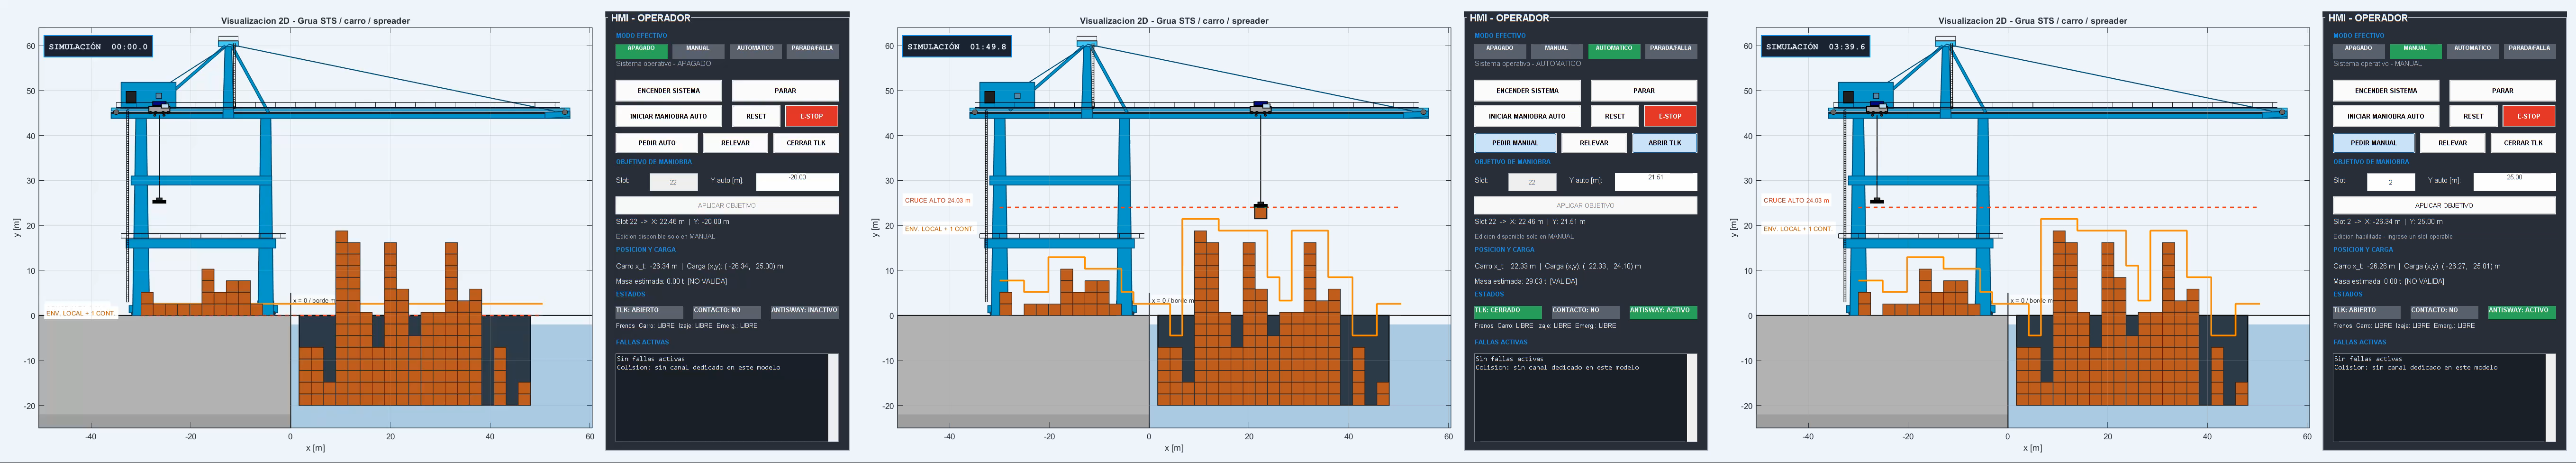
\includegraphics[width=.98\linewidth,height=4.6cm,keepaspectratio]{imagenes/video_inicial.png}\end{center}\begin{center}\href{run:videos/productividad_inicial_5x.mp4}{\textcolor{accent}{\textbf{Abrir video · reproducción 5× · 44 s}}}\end{center}
\note{Reproducir el video inicial y señalar las detenciones y etapas manuales. Abrir desde la carpeta videos si el visor PDF bloquea enlaces locales. La aceleración del video no altera el tiempo de simulación medido.}
\end{frame}
\begin{frame}[t,label=slide79]{Metodología de ajuste}
\begin{itemize}
\item 1. Revisar maniobras manuales y continuidad entre modos.
\item 2. Revisar márgenes geométricos y condiciones de supervisión.
\item 3. Ampliar límites y corregir casos del generador de trayectorias.
\item 4. Ajustar ganancias del carro y contribuciones anti-sway.
\item 5. Repetir el mismo ciclo y verificar entrega, perfil y regreso.
\end{itemize}
\note{La arquitectura regulatoria y el frenado conservan su estructura. Los resultados corresponden al conjunto de ajustes; no constituyen un barrido factorial para atribuir ahorros individuales.}
\end{frame}
\begin{frame}[t,label=slide80]{Operación manual y pesaje}
\begin{itemize}
\item Mayor velocidad manual con carga y en vacío; aproximación de unos 0,20 m/s.
\item Despegue lento de 0,15 m nominales para pesar.
\item Estabilidad de 0,25 s y promedio válido de 0,50 s.
\item Sin contacto ni cable flojo; $|v_y|<0,03$ m/s y $|a_y|<0,05$ m/s².
\item Solicitud de AUTO durante ascenso, cerca de 1 m/s, con referencias sincronizadas.
\end{itemize}
\note{Justificar que se evita parar antes de AUTO sin eliminar el pesaje estable. Se aplica también a la extracción vacía; el cambio de modo debe partir del estado medido.}
\end{frame}
\begin{frame}[t,label=slide81]{Geometría, llegada y vigilancia de seguimiento}
\begin{center}
{\small\renewcommand{\arraystretch}{1.0}
\begin{tabular}{lrr}\toprule
Parámetro & Inicial & Ajustado\\\midrule
Margen local sobre perfil [m] & 2,59 & 1,00\\
Umbral de ángulo & 0,005 rad & 0,5°\\
Umbral de velocidad angular [rad/s] & 0,012 & 0,050\\
Error horizontal vigilado [m] & 2,50 & 4,00\\
\bottomrule\end{tabular}}\end{center}
La trayectoria se vuelve a verificar sobre la huella completa de la carga.
\note{Los umbrales angulares son condiciones de llegada, no límites globales de balanceo durante todo el traslado. La vigilancia de seguimiento más amplia debe mencionarse explícitamente.}
\end{frame}
\begin{frame}[t,label=slide82]{Límites del generador y sintonía del carro}
\begin{columns}[T,onlytextwidth]
\column{0.49\textwidth}\begin{center}
{\small\renewcommand{\arraystretch}{1.0}
\begin{tabular}{lrr}\toprule
Generador & Inicial & Ajustado\\\midrule
$v_{x,max}$ [m/s] & 2,50 & 4,00\\
$a_{x,max}$ [m/s²] & 0,30 & 0,45\\
$a_{y,max}$ [m/s²] & 0,25 & 0,45\\
$j_x$ [m/s³] & 0,50 & 0,50\\
$j_y$ [m/s³] & 0,10 & 0,10\\
\bottomrule\end{tabular}}\end{center}

\column{0.47\textwidth}\begin{center}
{\small\renewcommand{\arraystretch}{1.0}
\begin{tabular}{lrr}\toprule
Ganancia & Inicial & Ajustado\\\midrule
$K_x$ & 0,20 & 0,25\\
$K_p$ & 2,40 & 3,20\\
$K_i$ & 0,20 & 0,267\\
Factor FB & 1,00 & 0,305\\
Factor FF & 1,00 & 0,340\\
\bottomrule\end{tabular}}\end{center}

\end{columns}\vspace{3mm}Se conservan jerk, velocidad de izaje en vacío de 3 m/s y regulación de izaje.\par $I_{max}=0,80/K_i=2,99625$ m; ganancias constantes durante el frenado.
\note{Además se corrigió la rampa horizontal que no alcanza velocidad máxima y se afinó la búsqueda de duración vertical. El límite por masa y potencia permanece; no cambia la arquitectura regulatoria.}
\end{frame}
\begin{frame}[t,label=slide83]{Prueba de ciclo ajustado: posiciones y velocidades}
\relax
\figurefooter{Tiempo referido al inicio del ciclo; altura física del spreader y velocidad de izaje del accionamiento.}
\vspace{-2mm}\makebox[\linewidth][c]{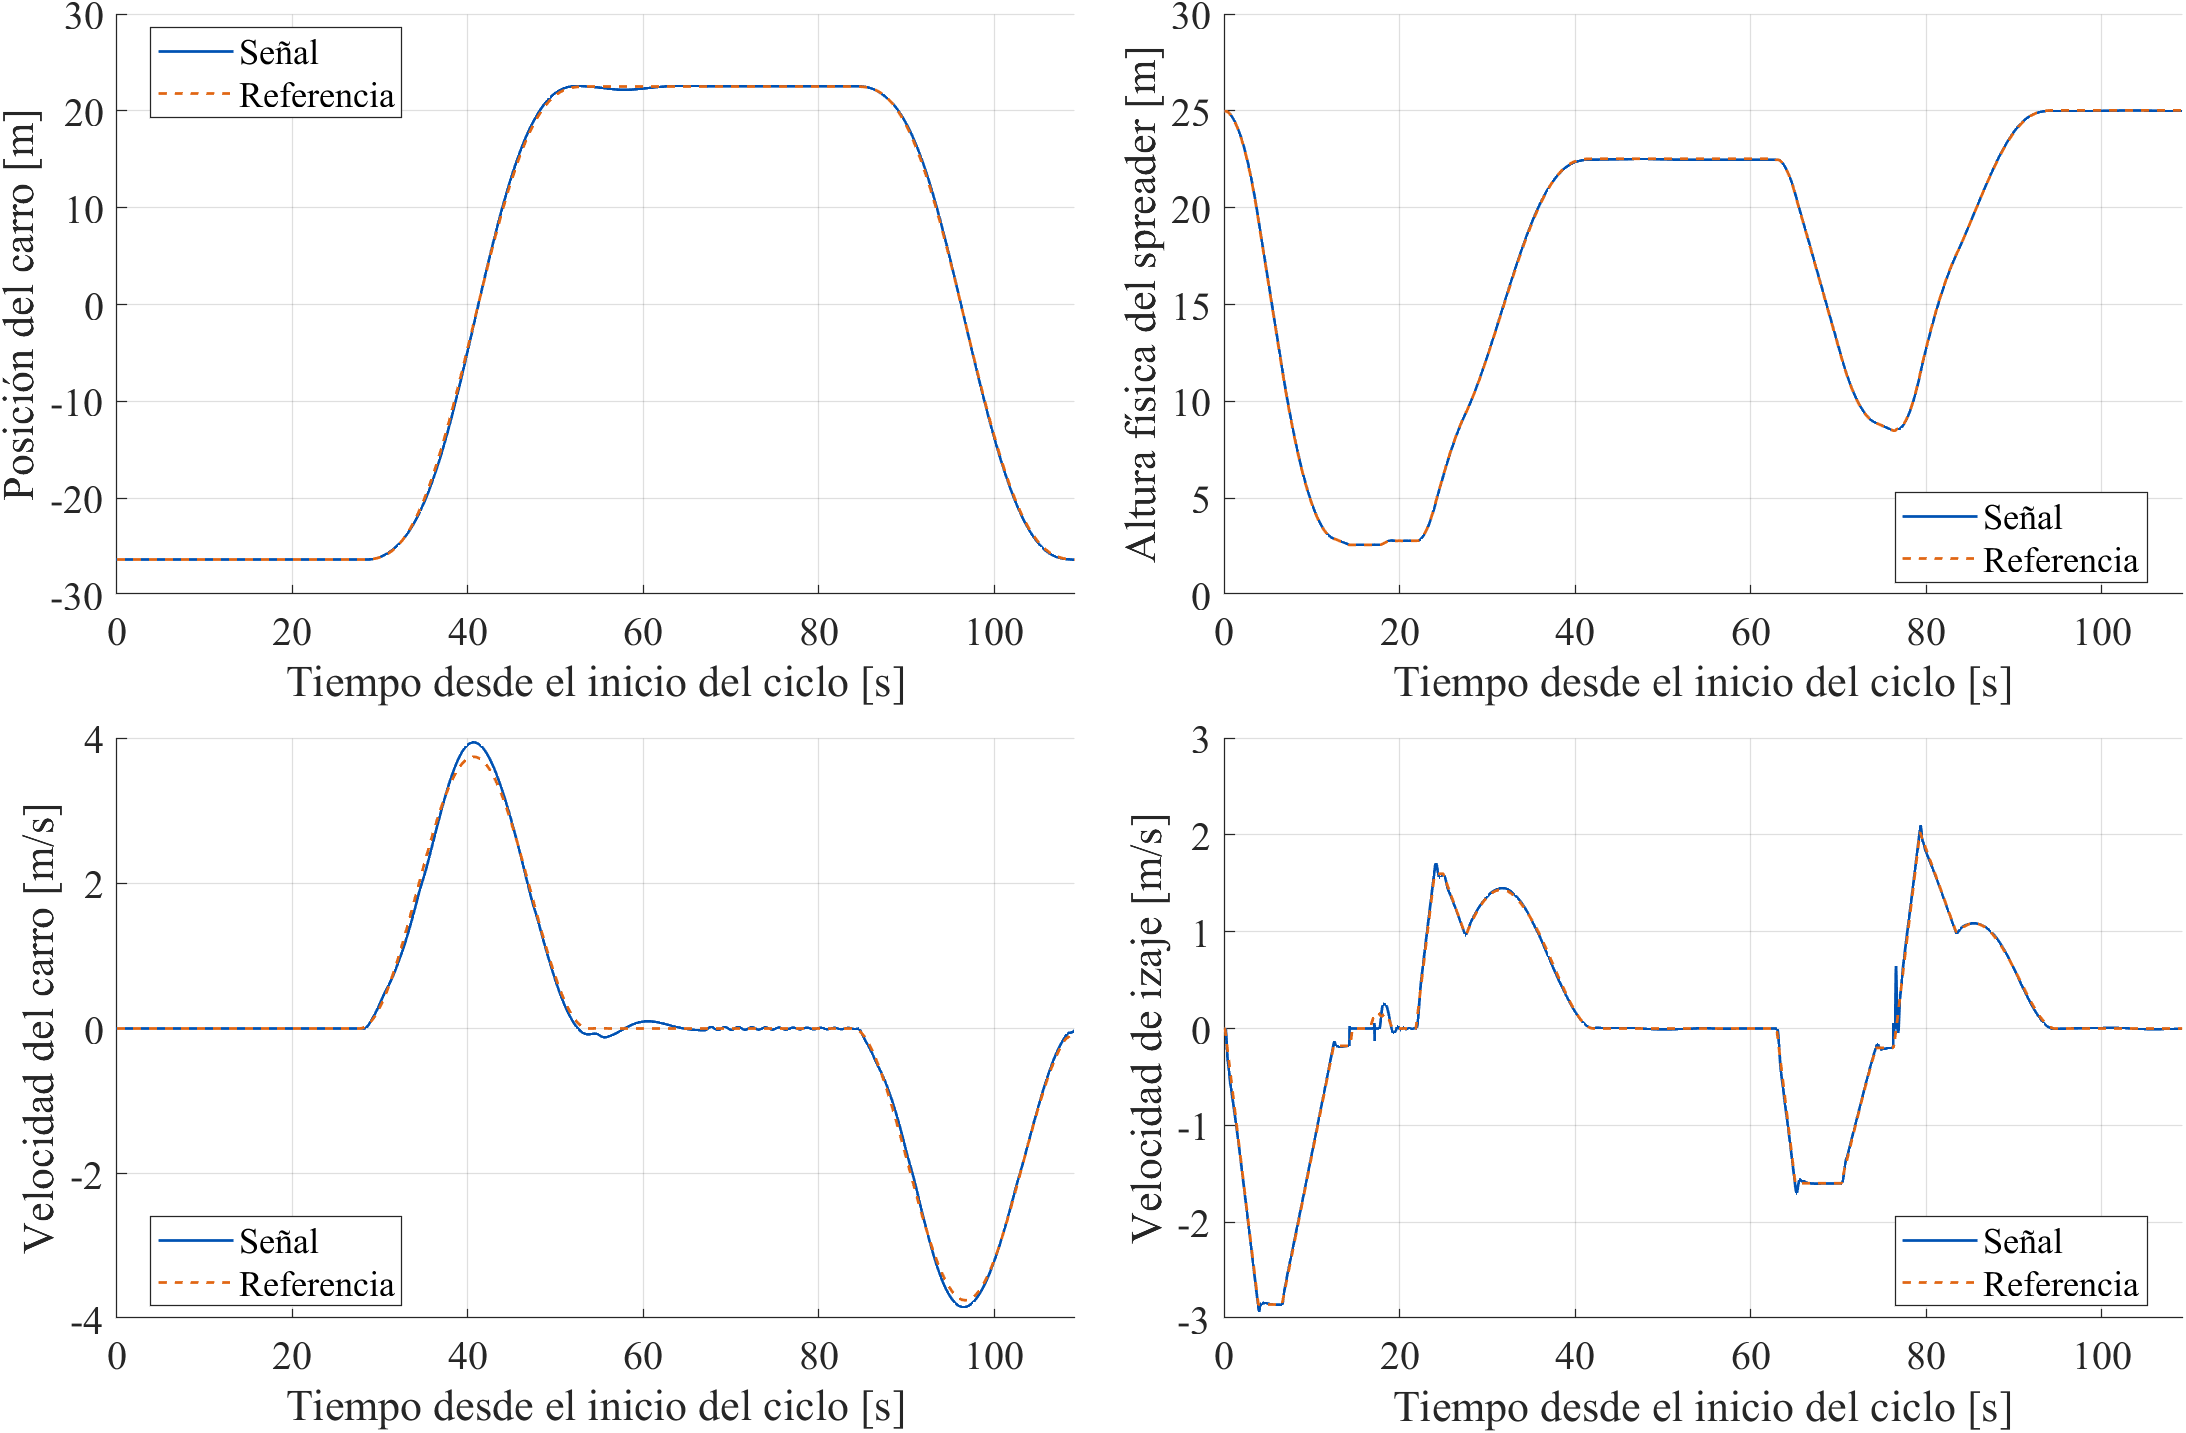
\includegraphics[width=15.0cm,height=6.05cm,keepaspectratio,trim=0.00bp 0.00bp 0.00bp 0.00bp,clip]{imagenes/r_082.png}}\par\note{Mostrar continuidad al iniciar AUTO y retorno combinado en x y altura. La confirmación de regreso ocurre a111,16 absoluto,109,16desdeinicio.}
\end{frame}
\begin{frame}[t,label=slide84]{Prueba de ciclo ajustado: recorrido y perfil}
\relax
\figurefooter{Traslado cargado y retorno vacío sobre perfiles actualizados.}
\vspace{-2mm}\makebox[\linewidth][c]{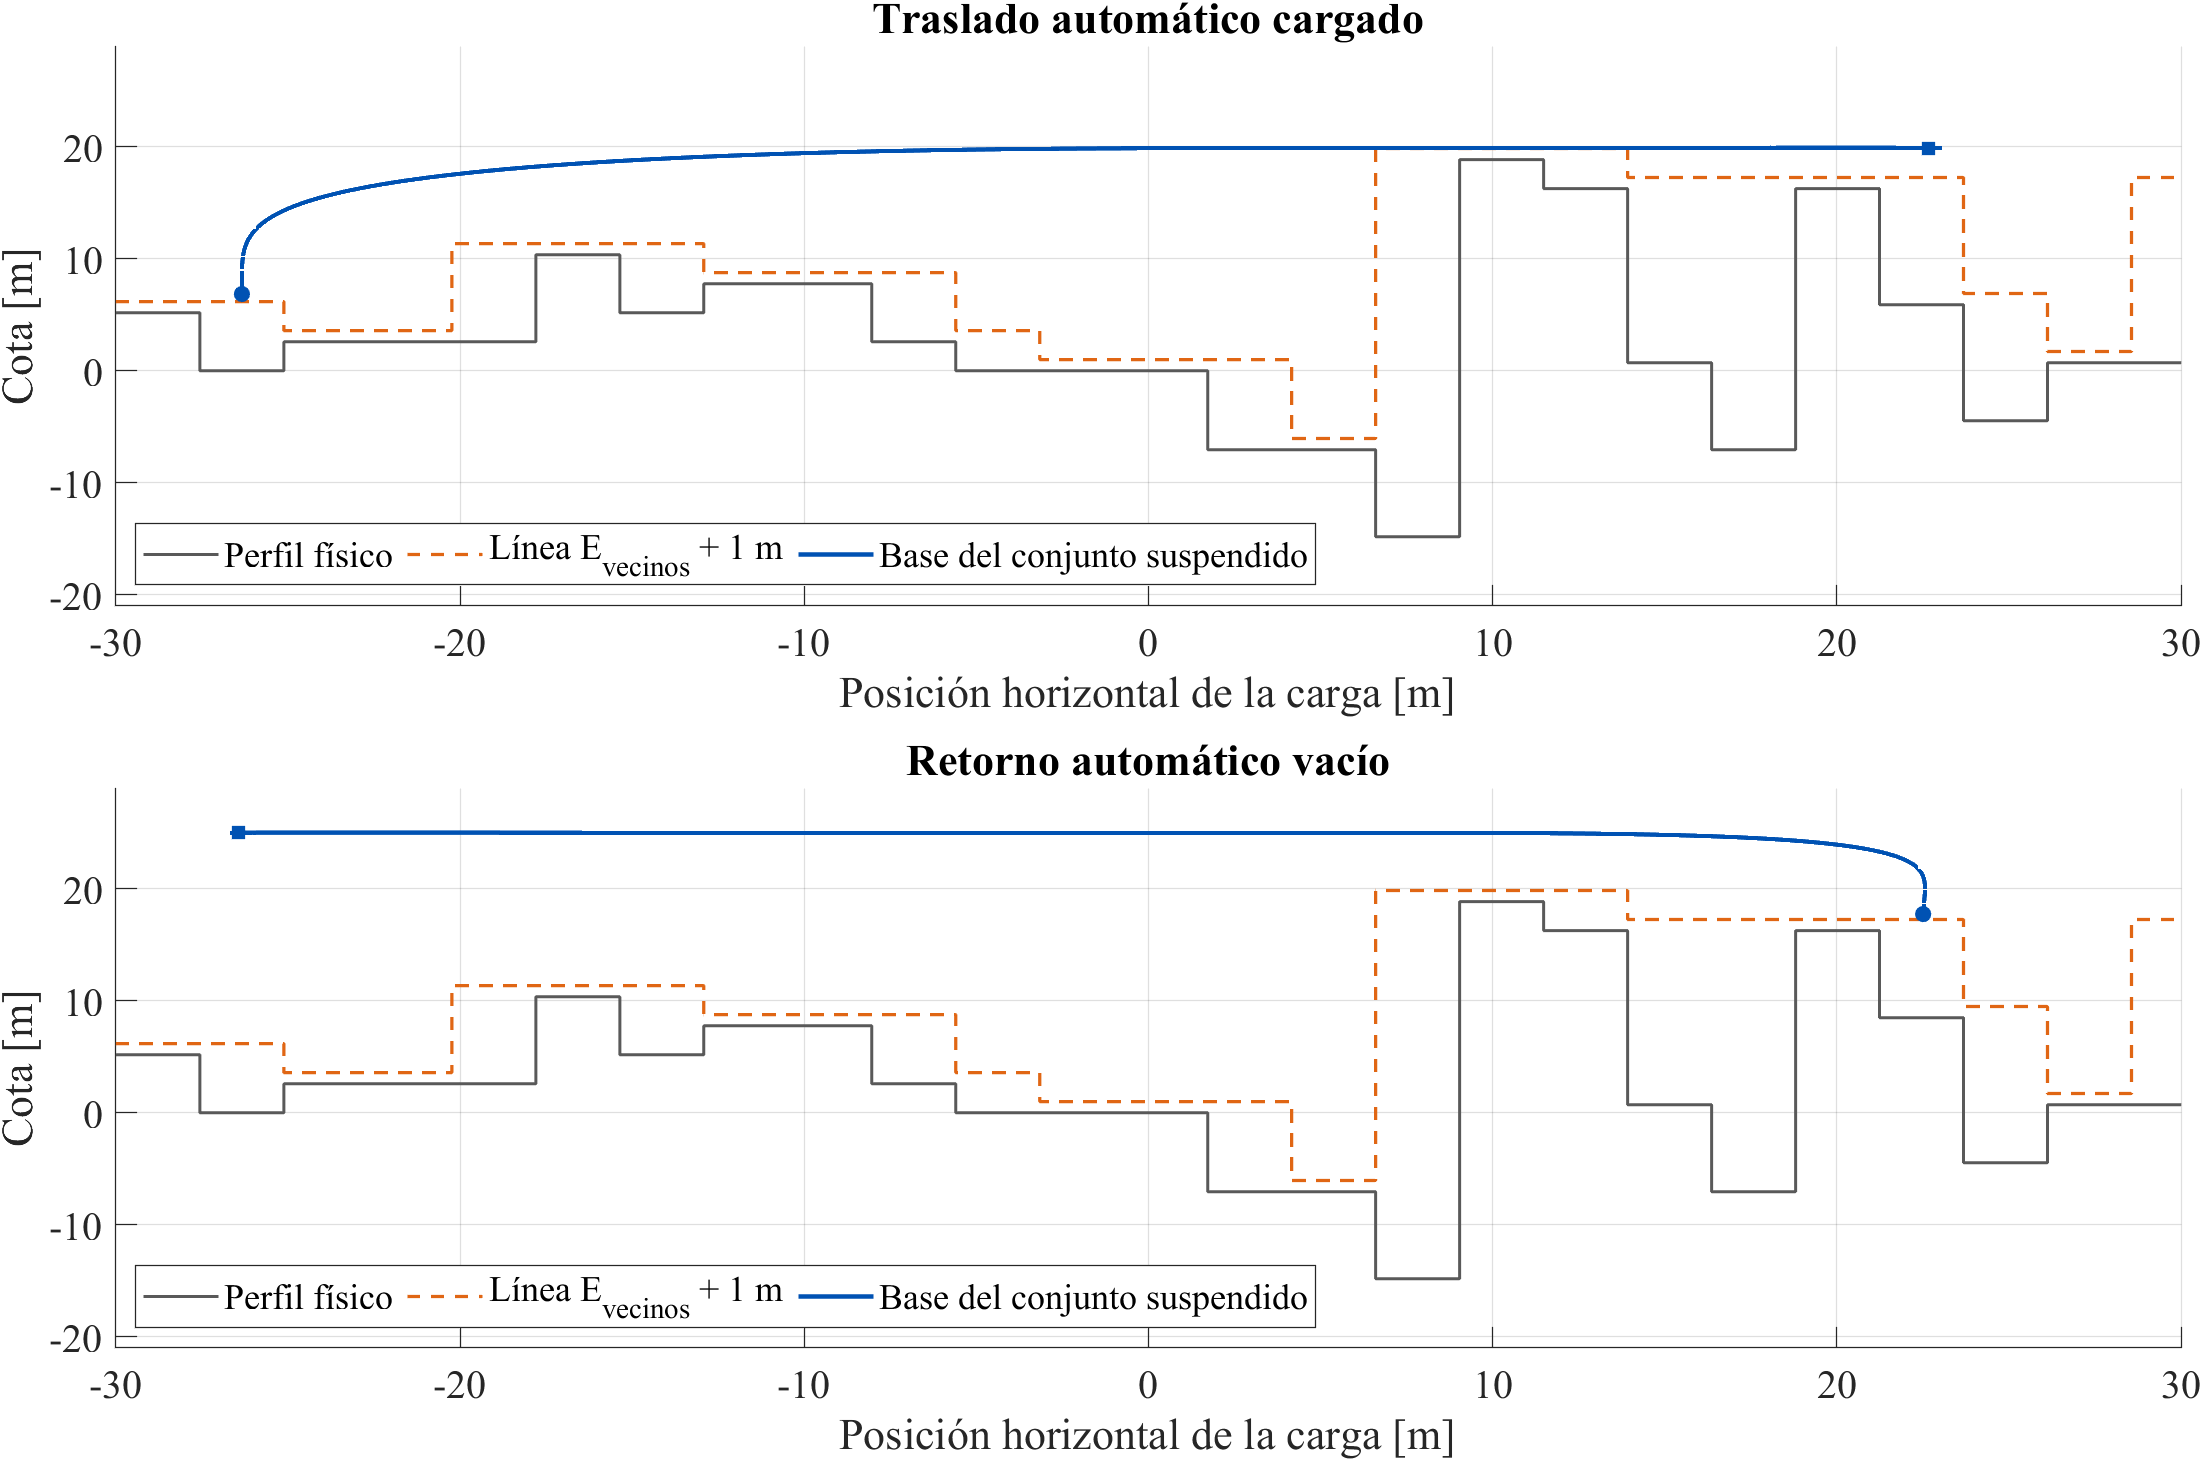
\includegraphics[width=15.0cm,height=6.05cm,keepaspectratio,trim=0.00bp 0.00bp 0.00bp 0.00bp,clip]{imagenes/r_083.png}}\par\note{La base cargada se obtiene restando Hc a la altura física. Margen mínimo bajo toda la huella enAUTO:0,0417m cargado y0,4816m vacío. Indicar que se verifica el caso simulado.}
\end{frame}
\begin{frame}[t,label=slide85]{Prueba de ciclo ajustado: balanceo y llegada}
\begin{center}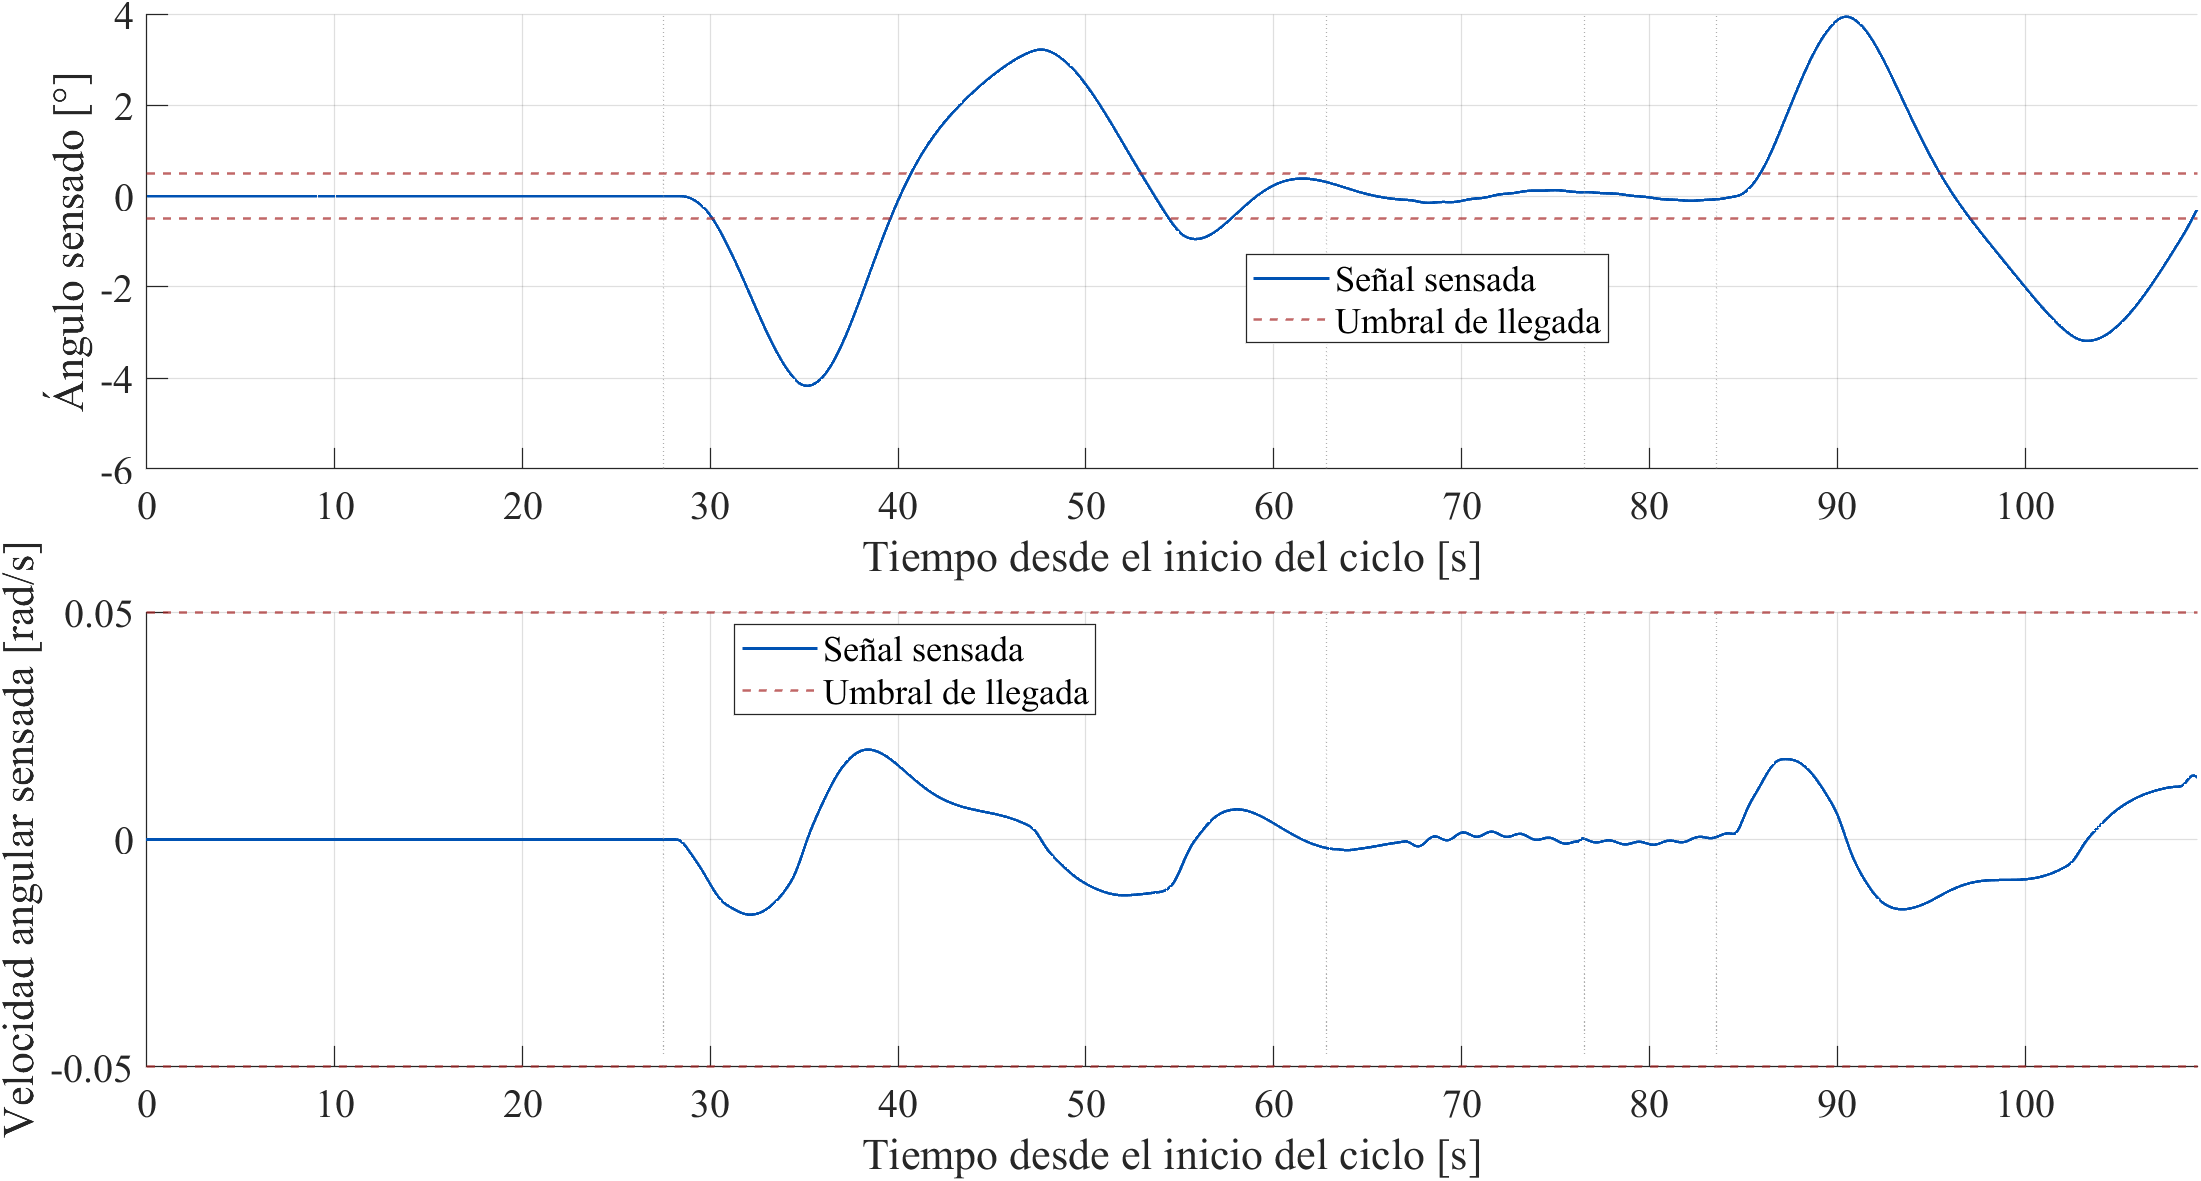
\includegraphics[width=.98\linewidth,height=5.55cm,keepaspectratio]{imagenes/r_084.png}\end{center}\vspace{-1mm}\figcaption{Los umbrales dibujados se verifican en llegada junto con posición y velocidad horizontal.}
\note{No presentar los umbrales como una banda que deba cumplirse durante todo el transporte. Las líneas verticales identifican solicitudes de modos, entrega y retorno.}
\end{frame}
\begin{frame}[t,label=slide86]{Prueba de ciclo cerrado: comparación por etapa}
\begin{center}
{\small\renewcommand{\arraystretch}{1.0}
\begin{tabular}{lrr}\toprule
Etapa & Inicial [s] & Ajustado [s]\\\midrule
Descenso vacío & 37,72 & 14,32\\
Twistlocks & 1,04 & 1,04\\
Extracción y pesaje & 23,88 & 12,16\\
AUTO cargado & 55,76 & 35,28\\
Manual y entrega & 30,72 & 13,72\\
Extracción vacía & 22,00 & 7,04\\
AUTO vacío & 46,52 & 25,36\\
Reposo final & 0,28 & 0,24\\
\textbf{Total} & \textbf{217,92} & \textbf{109,16}\\
\bottomrule\end{tabular}}\end{center}
Ahorro conjunto: 108,76 s (49,91 \%).
\note{Las fronteras de etapa son las mismas que en el cálculo inicial. Resaltar que los ahorros se distribuyen entre operación y traslados, sin atribuir toda la mejora al PI.}
\end{frame}
\begin{frame}[t,label=slide87]{Prueba de ciclo ajustado: productividad estimada}
\[
T_1=111{,}16-2{,}00=109{,}16\ \mathrm{s}
\]
\[
\boxed{P_1=\frac{3600}{109{,}16}=32{,}98\ \mathrm{contenedores/h}}
\]
\begin{itemize}
\item Margen temporal respecto del objetivo: 10,84 s.
\item Entrega y cambios de perfil verificados; retorno vacío a altura 24,9886 m.
\item Cumplimiento para el recorrido, masa y condiciones evaluados.
\item Otros recorridos y demoras logísticas requieren evaluación adicional.
\end{itemize}
\note{Diferenciar productividad estimada del cicloMIL de productividad portuaria sostenida. La sintonía ajustada no queda validada en los dos traslados del ensayo completo anterior.}
\end{frame}
\begin{frame}[t,label=slide88]{Prueba de ciclo ajustado: video HMI}
\begin{center}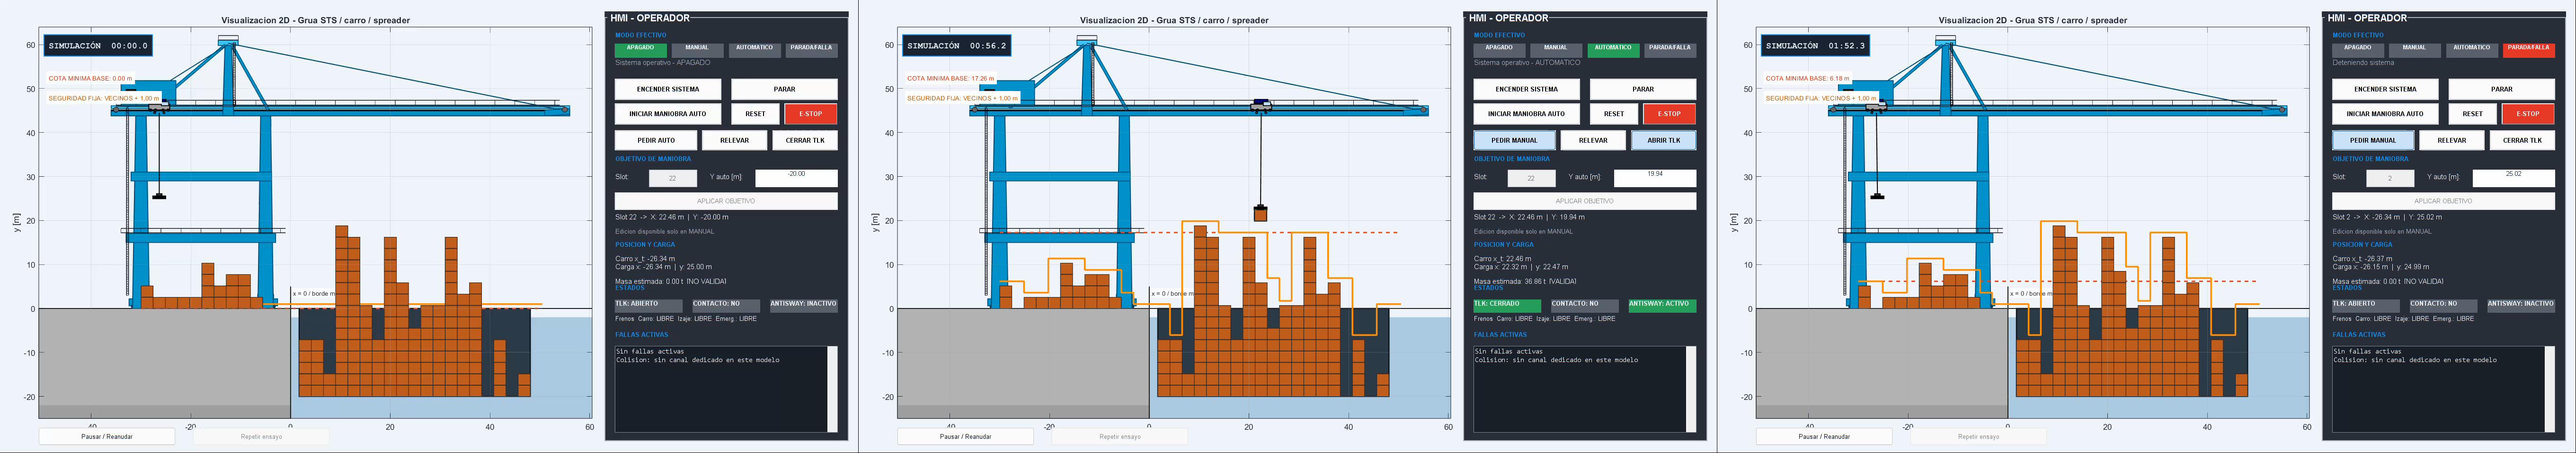
\includegraphics[width=.98\linewidth,height=4.6cm,keepaspectratio]{imagenes/video_ajustado.png}\end{center}\begin{center}\href{run:videos/productividad_ajustado_5x.mp4}{\textcolor{accent}{\textbf{Abrir video · reproducción 5× · 23 s}}}\end{center}
\note{Reproducir y relacionar la continuidad entre modos con las trayectorias recién mostradas. El tiempo de reproducción es22,6s y el video contiene112,8sdesimulación.}
\end{frame}
\section{Conclusiones}
\begin{frame}[plain,label=seccion10]
\setbeamertemplate{frametitle}{}
\vfill
{\fontsize{25}{29}\selectfont\bfseries Conclusiones y trabajos futuros\par}
\vspace{4mm}\textcolor{accent}{\rule{.75\linewidth}{1pt}}\par\vspace{3mm}
{\large Resultados del proyecto y próximos desarrollos.\par}\vfill
\note{Ubicar este bloque en el recorrido y anunciar su objetivo.}
\end{frame}
\begin{frame}[t,label=slide89]{Resultados principales del proyecto}
\begin{itemize}
\item Sistema jerárquico integrado con planta no lineal, regulación y secuencias.
\item Control de balanceo que permite cumplir las condiciones de llegada.
\item Diagnóstico mecánico y corrección de la excitación en la parada manual.
\item Migración a CODESYS y realización equivalente de la regulación en MC.
\item Pruebas completas MIL y SIL; ciclo ajustado de 109,16 s.
\end{itemize}
\note{Retomar los objetivos iniciales con resultados concretos. No repetir todas las métricas: elegir0,627m/s²,97,8\%y32,98cont/hsegúneltiempo.}
\end{frame}

\begin{frame}[t,label=trabajosfuturos]{Trabajos futuros}
\relax
\begin{itemize}
\item \textbf{Completar situaciones de seguridad pendientes:} fallas simultáneas y arranque con finales de carrera activos.
\item \textbf{Ampliar la evaluación de productividad:} otras masas, recorridos y perfiles, mediante pruebas completas.
\item \textbf{Optimizar la trayectoria coordinada:} iniciar antes el descenso cuando la geometría y la seguridad lo permitan, aumentando el solapamiento entre ejes.
\item \textbf{Evaluar otras estrategias de control:} LQR, MPC y controles no lineales; comparar seguimiento, balanceo, esfuerzo y cumplimiento de restricciones.
\end{itemize}
\note{La optimización busca reducir el tiempo de ciclo mediante mayor simultaneidad entre traslado y descenso, respetando obstáculos y condiciones de llegada. El generador ya coordina ejes: se propone refinar el inicio de descenso, no introducir por primera vez coordinación. Comparar estrategias con las mismas maniobras y restricciones. Se retiraron los trabajos de watchdog, ruido e incertidumbre, y validación de hardware acordados con el usuario.}
\end{frame}

\begin{frame}[t,label=slide91]{Preguntas}
\vfill\textcolor{accent}{\Large Automatización y Control de una Grúa Portuaria STS}\par\vspace{5mm}Matías Escobar · Martín Herrera\par\vfill
\note{Abrir el coloquio. Usar las diapositivas de respaldo para responder con ecuaciones, diagramas y gráficas adicionales.}
\end{frame}
\appendix\metroset{numbering=none,progressbar=none}
\section{Respaldo técnico}
\begin{frame}[t,label=pendulodeduccion]{Respaldo: deducción angular del carro y péndulo}
\relax
{\small
\[
\mathcal T=\frac{m_l}{2}\left[\dot x_t^2+\dot l^2+l^2\dot\theta_l^2
+2\dot x_t\dot l\sin\theta_l+2\dot x_tl\dot\theta_l\cos\theta_l\right]
\]
\[
\mathcal V=m_lg(45-l\cos\theta_l),\qquad
\frac{d}{dt}\frac{\partial(\mathcal T-\mathcal V)}{\partial\dot\theta_l}
-\frac{\partial(\mathcal T-\mathcal V)}{\partial\theta_l}=0
\]
\[
m_ll^2\ddot\theta_l+2m_ll\dot l\dot\theta_l
+m_ll\ddot x_t\cos\theta_l+m_lgl\sin\theta_l=0
\]
}
Dividir por $m_ll$ recupera la ecuación angular. El término radial de tensión no aporta par respecto del punto de suspensión.
\note{La masa se cancela en esta ecuación pendular ideal. El contacto puede agregar fuerza tangencial y el cambio de masa se trata como evento fuera de esta deducción.}
\end{frame}
\begin{frame}[t,label=slide92]{Respaldo: energías y ecuación pendular}
\[
\begin{aligned}x_l&=x_t+l\sin\theta_l,&y_l&=45-l\cos\theta_l,\\\dot x_l&=\dot x_t+\dot l\sin\theta_l+l\dot\theta_l\cos\theta_l,\\\dot y_l&=-\dot l\cos\theta_l+l\dot\theta_l\sin\theta_l.\end{aligned}
\]
\[
\mathcal T=\tfrac12m_l(\dot x_l^2+\dot y_l^2),\qquad \mathcal V=m_lg(45-l\cos\theta_l)
\]
\[
\frac{d}{dt}\frac{\partial(\mathcal T-\mathcal V)}{\partial\dot\theta_l}-\frac{\partial(\mathcal T-\mathcal V)}{\partial\theta_l}=0
\]
\[
l\ddot\theta_l+2\dot l\dot\theta_l+g\sin\theta_l=-\ddot x_t\cos\theta_l
\]

\note{Usar sólo si se pregunta por la derivación de Euler–Lagrange o por el acoplamiento del izaje con el balanceo.}
\end{frame}
\begin{frame}[t,label=slide93]{Respaldo: polinomio y ganancias del izaje}
\[
\alpha_h=\frac{i_h}{r_{hd}M_{EQh}},\quad \beta_h=\frac{b_{EQh}}{M_{EQh}}
\]
\[
P_h(s)=s^3+(\beta_h-\alpha_hK_{hd})s^2-\alpha_hK_{hp}s-\alpha_hK_{hi}
\]
\[
P_d(s)=s^3+n_h\omega_{posh}s^2+n_h\omega_{posh}^2s+\omega_{posh}^3
\]
La anticipación de la trayectoria no modifica el polinomio característico de la realimentación.
\note{Mostrar igualdad de coeficientes y el signo negativo que aparece al formular la dinámica en longitud.}
\end{frame}
\begin{frame}[t,label=slide94]{Respaldo: diagrama de operación}
\relax
\figurefooter{Vista de conjunto de la operación; las etapas se desglosan en el bloque comparativo.}
\vspace{-2mm}\makebox[\linewidth][c]{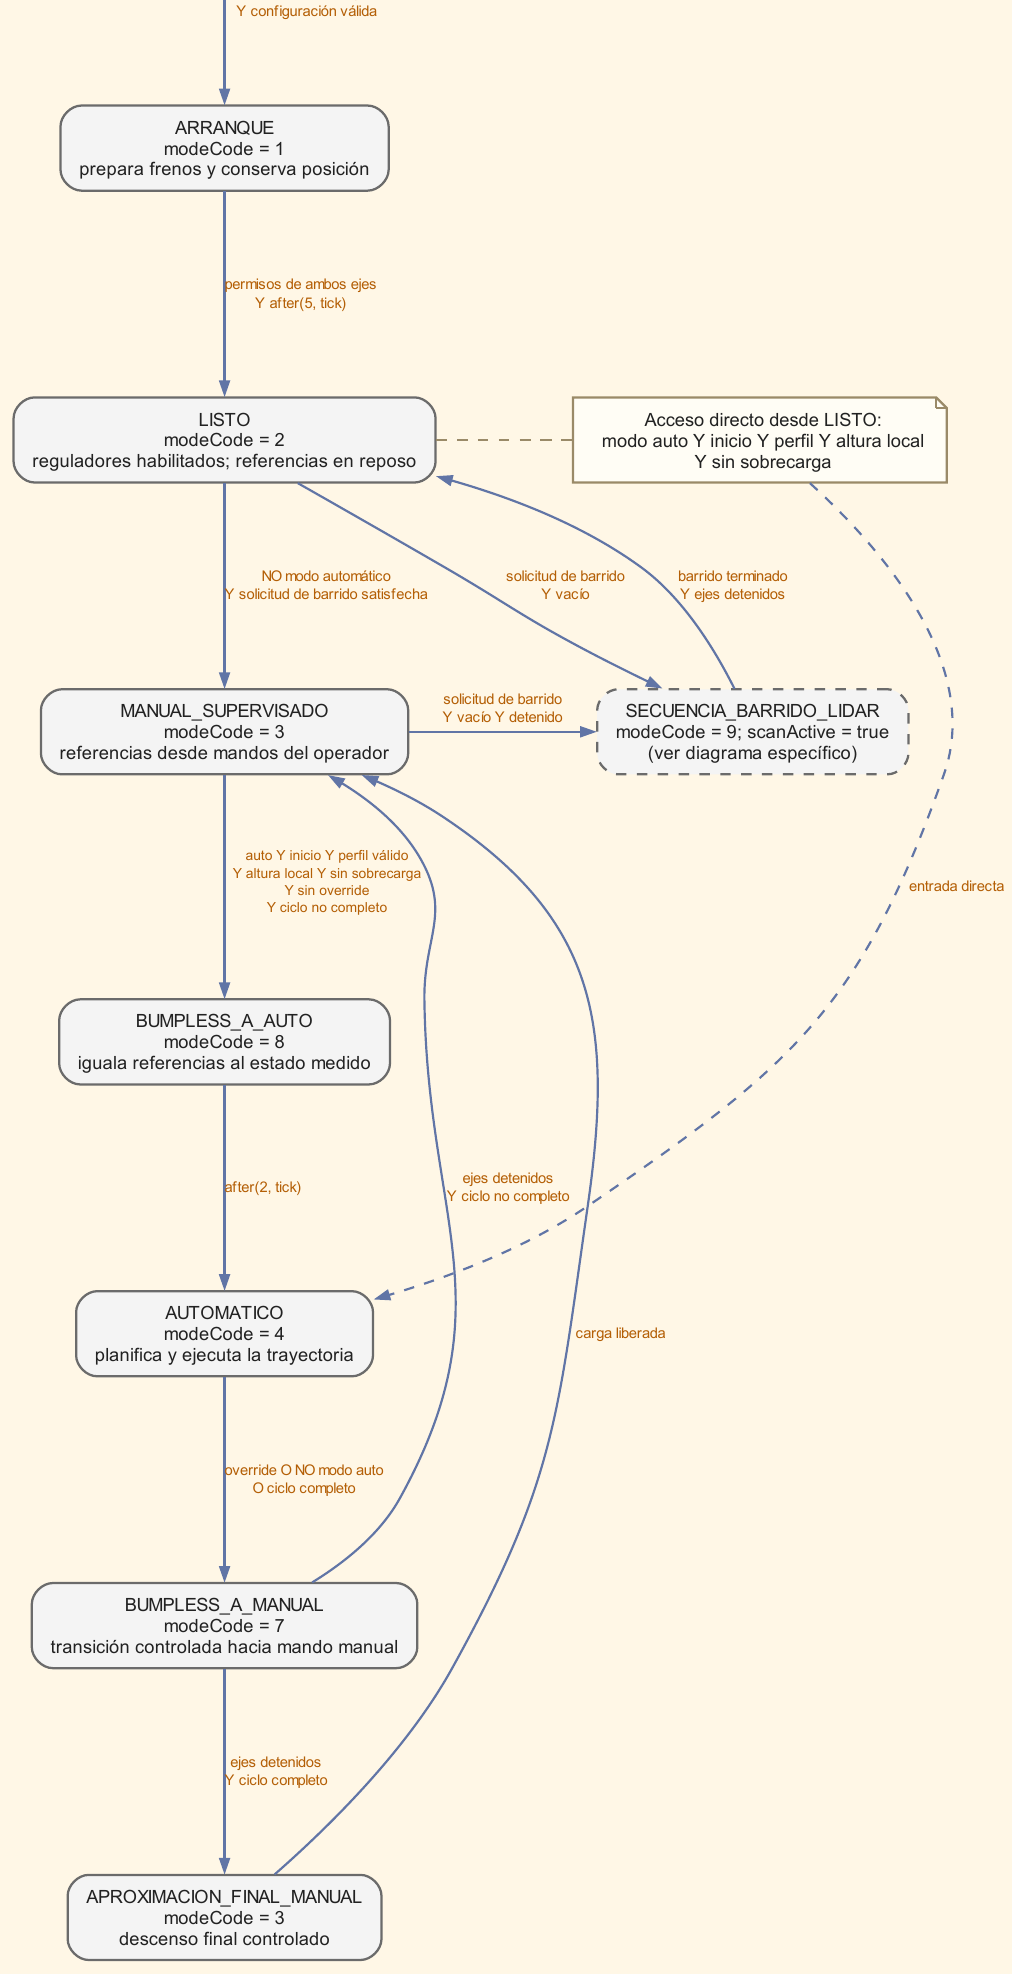
\includegraphics[width=15.0cm,height=6.35cm,keepaspectratio,trim=7.00bp 7.00bp 3.00bp 0.00bp,clip]{imagenes/r_027.png}}\par\note{Consultar las etapas desglosadas y sus guardas en el bloque comparativo.}
\end{frame}
\begin{frame}[t,label=slide95]{Respaldo: secuencia de carga y twistlocks}
\relax
\figurefooter{Máquina completa de toma, pesaje, entrega y retención.}
\vspace{-2mm}\makebox[\linewidth][c]{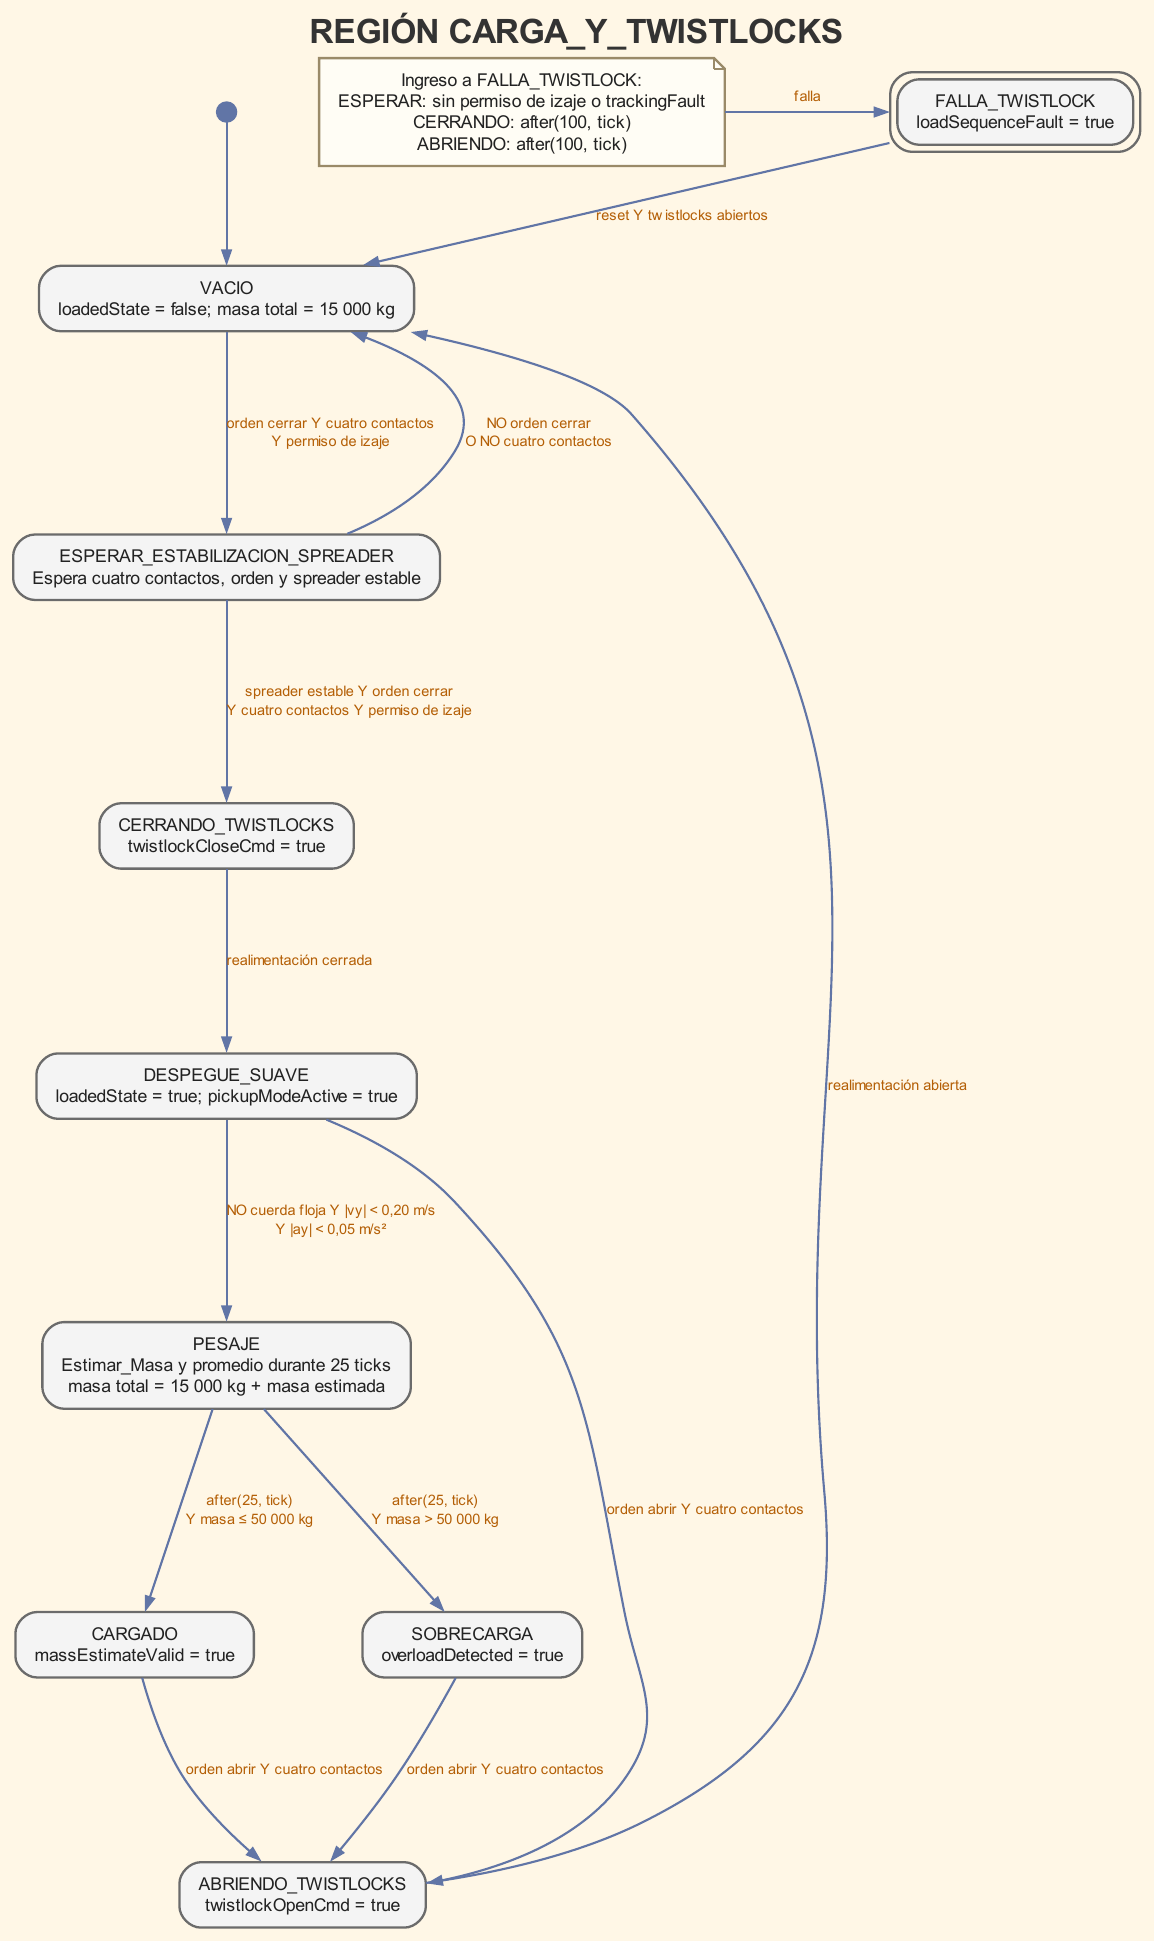
\includegraphics[width=15.0cm,height=6.35cm,keepaspectratio,trim=7.00bp 7.00bp 7.00bp 7.00bp,clip]{imagenes/r_031.png}}\par\note{Consultar ante preguntas sobre validación de masa, tiempos o bloqueo de twistlocks.}
\end{frame}
\begin{frame}[t,label=slide96]{Respaldo: secuencias de frenos}
\relax
\figurefooter{Máquinas paralelas de carro e izaje.}
\vspace{-2mm}\makebox[\linewidth][c]{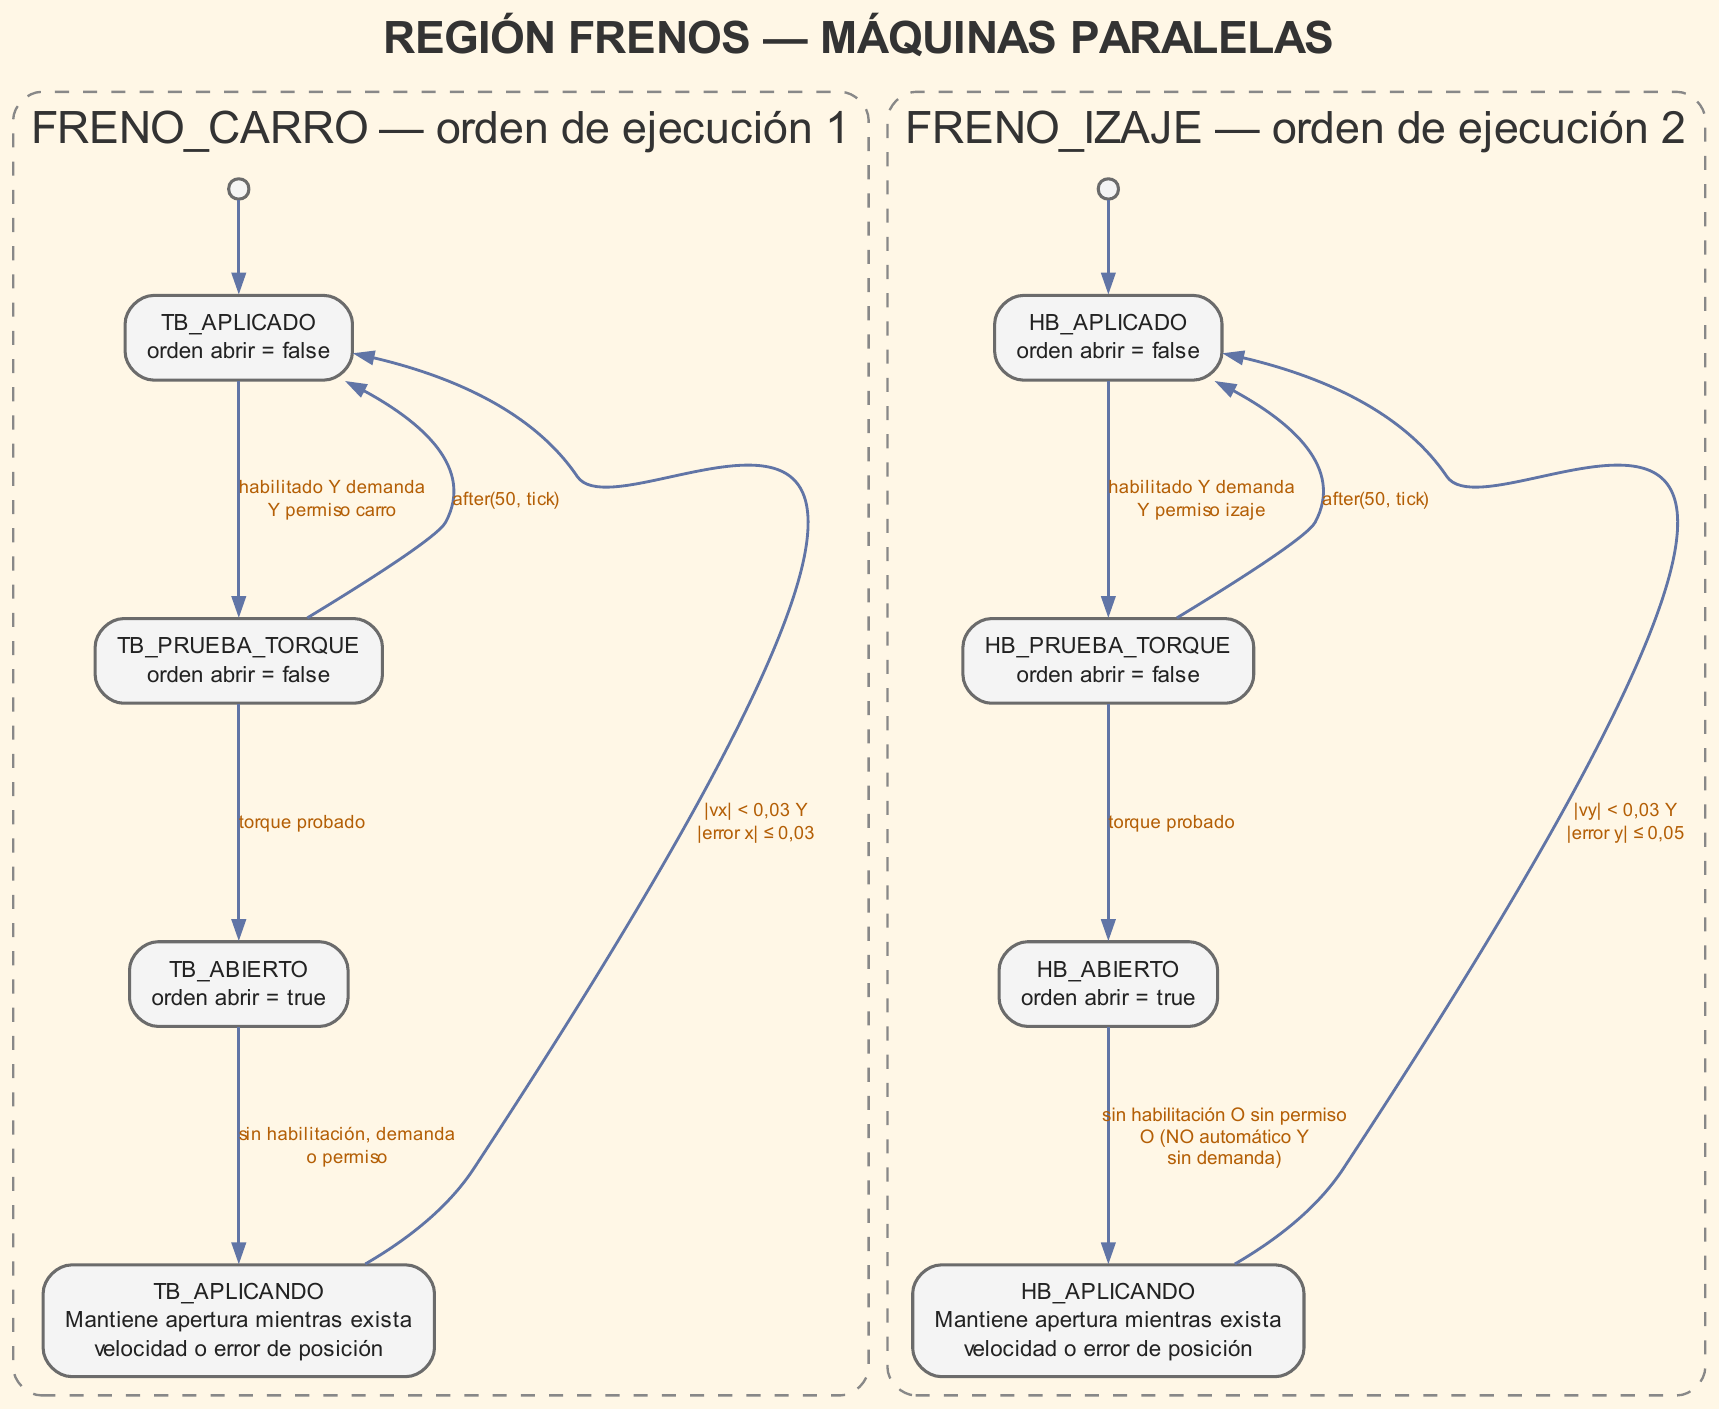
\includegraphics[width=15.0cm,height=6.35cm,keepaspectratio,trim=7.00bp 7.00bp 7.00bp 7.00bp,clip]{imagenes/r_032.png}}\par\note{Explicar el orden habilitación–torque–liberación y la verificación de respuesta.}
\end{frame}
\begin{frame}[t,label=slide97]{Respaldo: emergencias y rearme}
\relax
\figurefooter{Stateflow: prioridades, autorizaciones de freno y recuperación enclavada.}
\vspace{-2mm}\makebox[\linewidth][c]{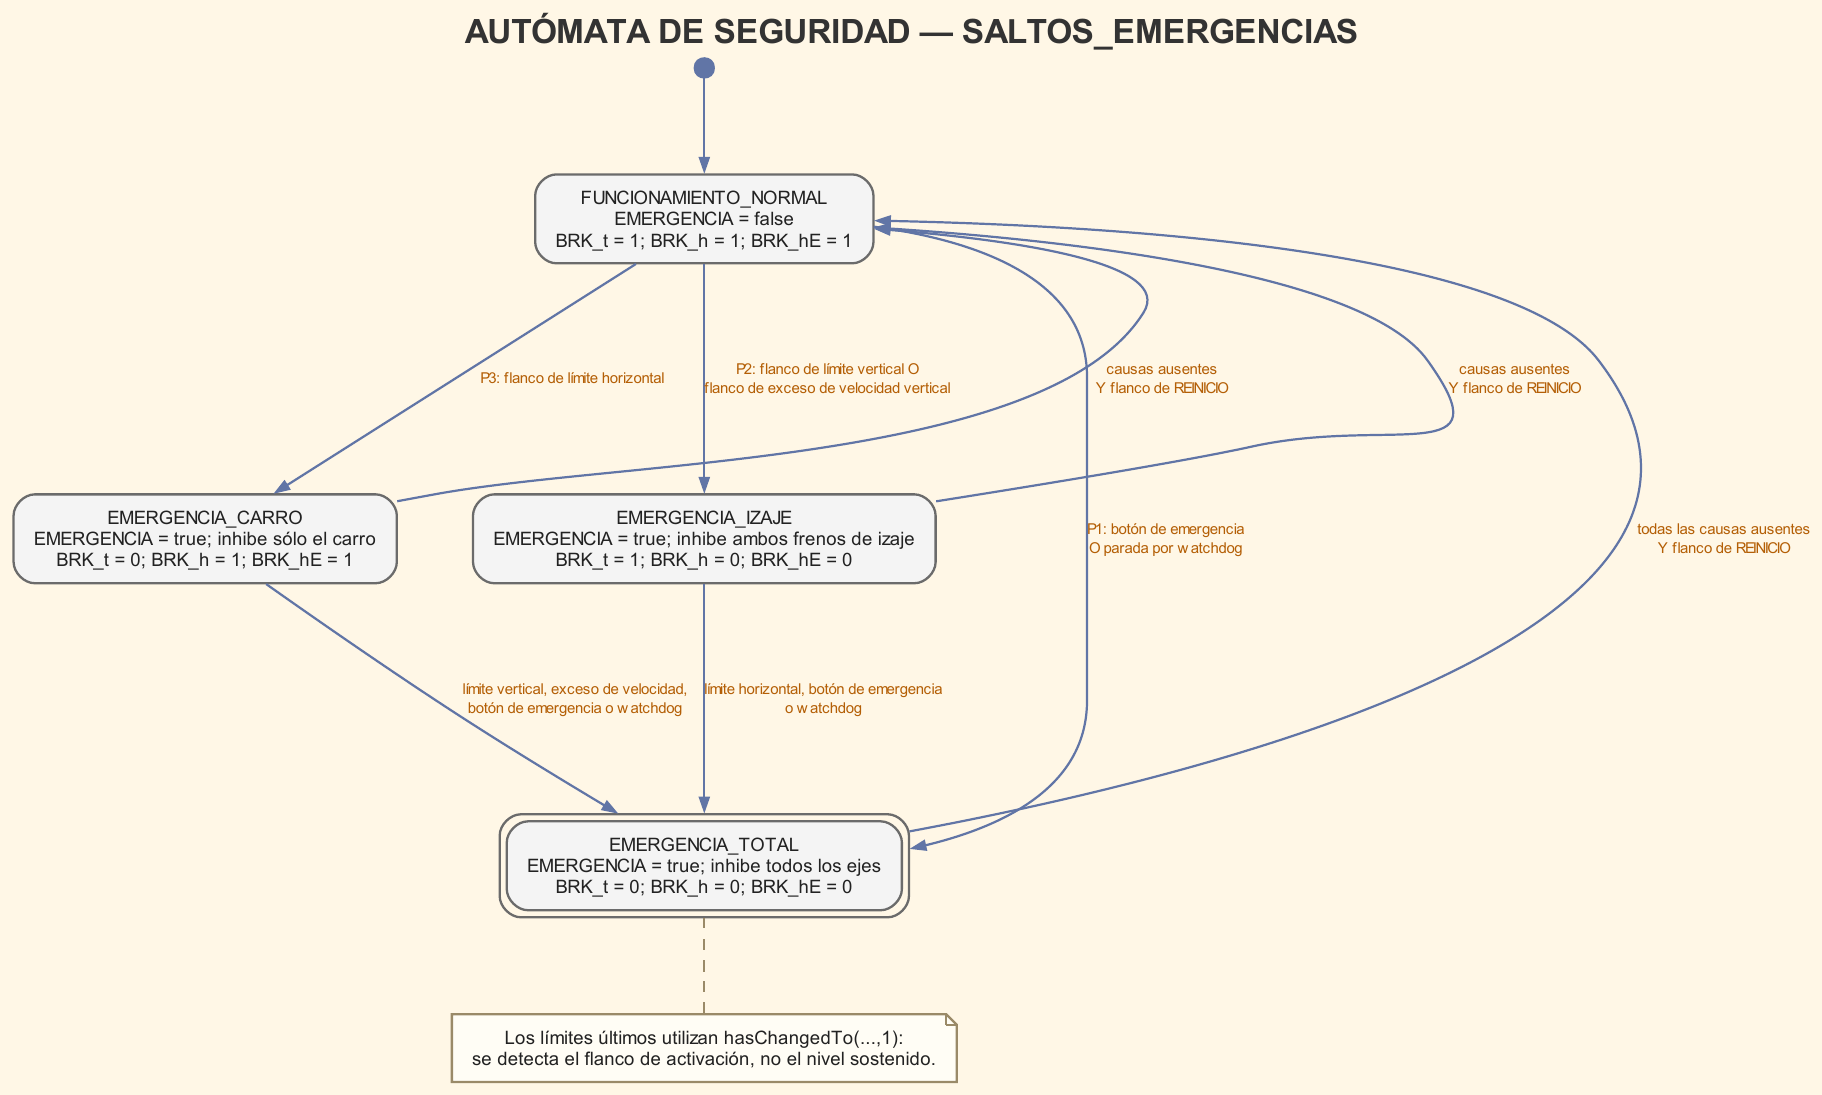
\includegraphics[width=15.0cm,height=6.35cm,keepaspectratio,trim=7.00bp 7.00bp 7.00bp 7.00bp,clip]{imagenes/r_035.png}}\par\note{Consultar para explicar el defecto de eventos simultáneos y la evaluación por flancos.}
\end{frame}
\begin{frame}[t,label=slide98]{Respaldo: SFC de operación en CODESYS}
\relax
\figurefooter{Implementación manual: pasos, acciones y guardas exportadas.}
\vspace{-2mm}\makebox[\linewidth][c]{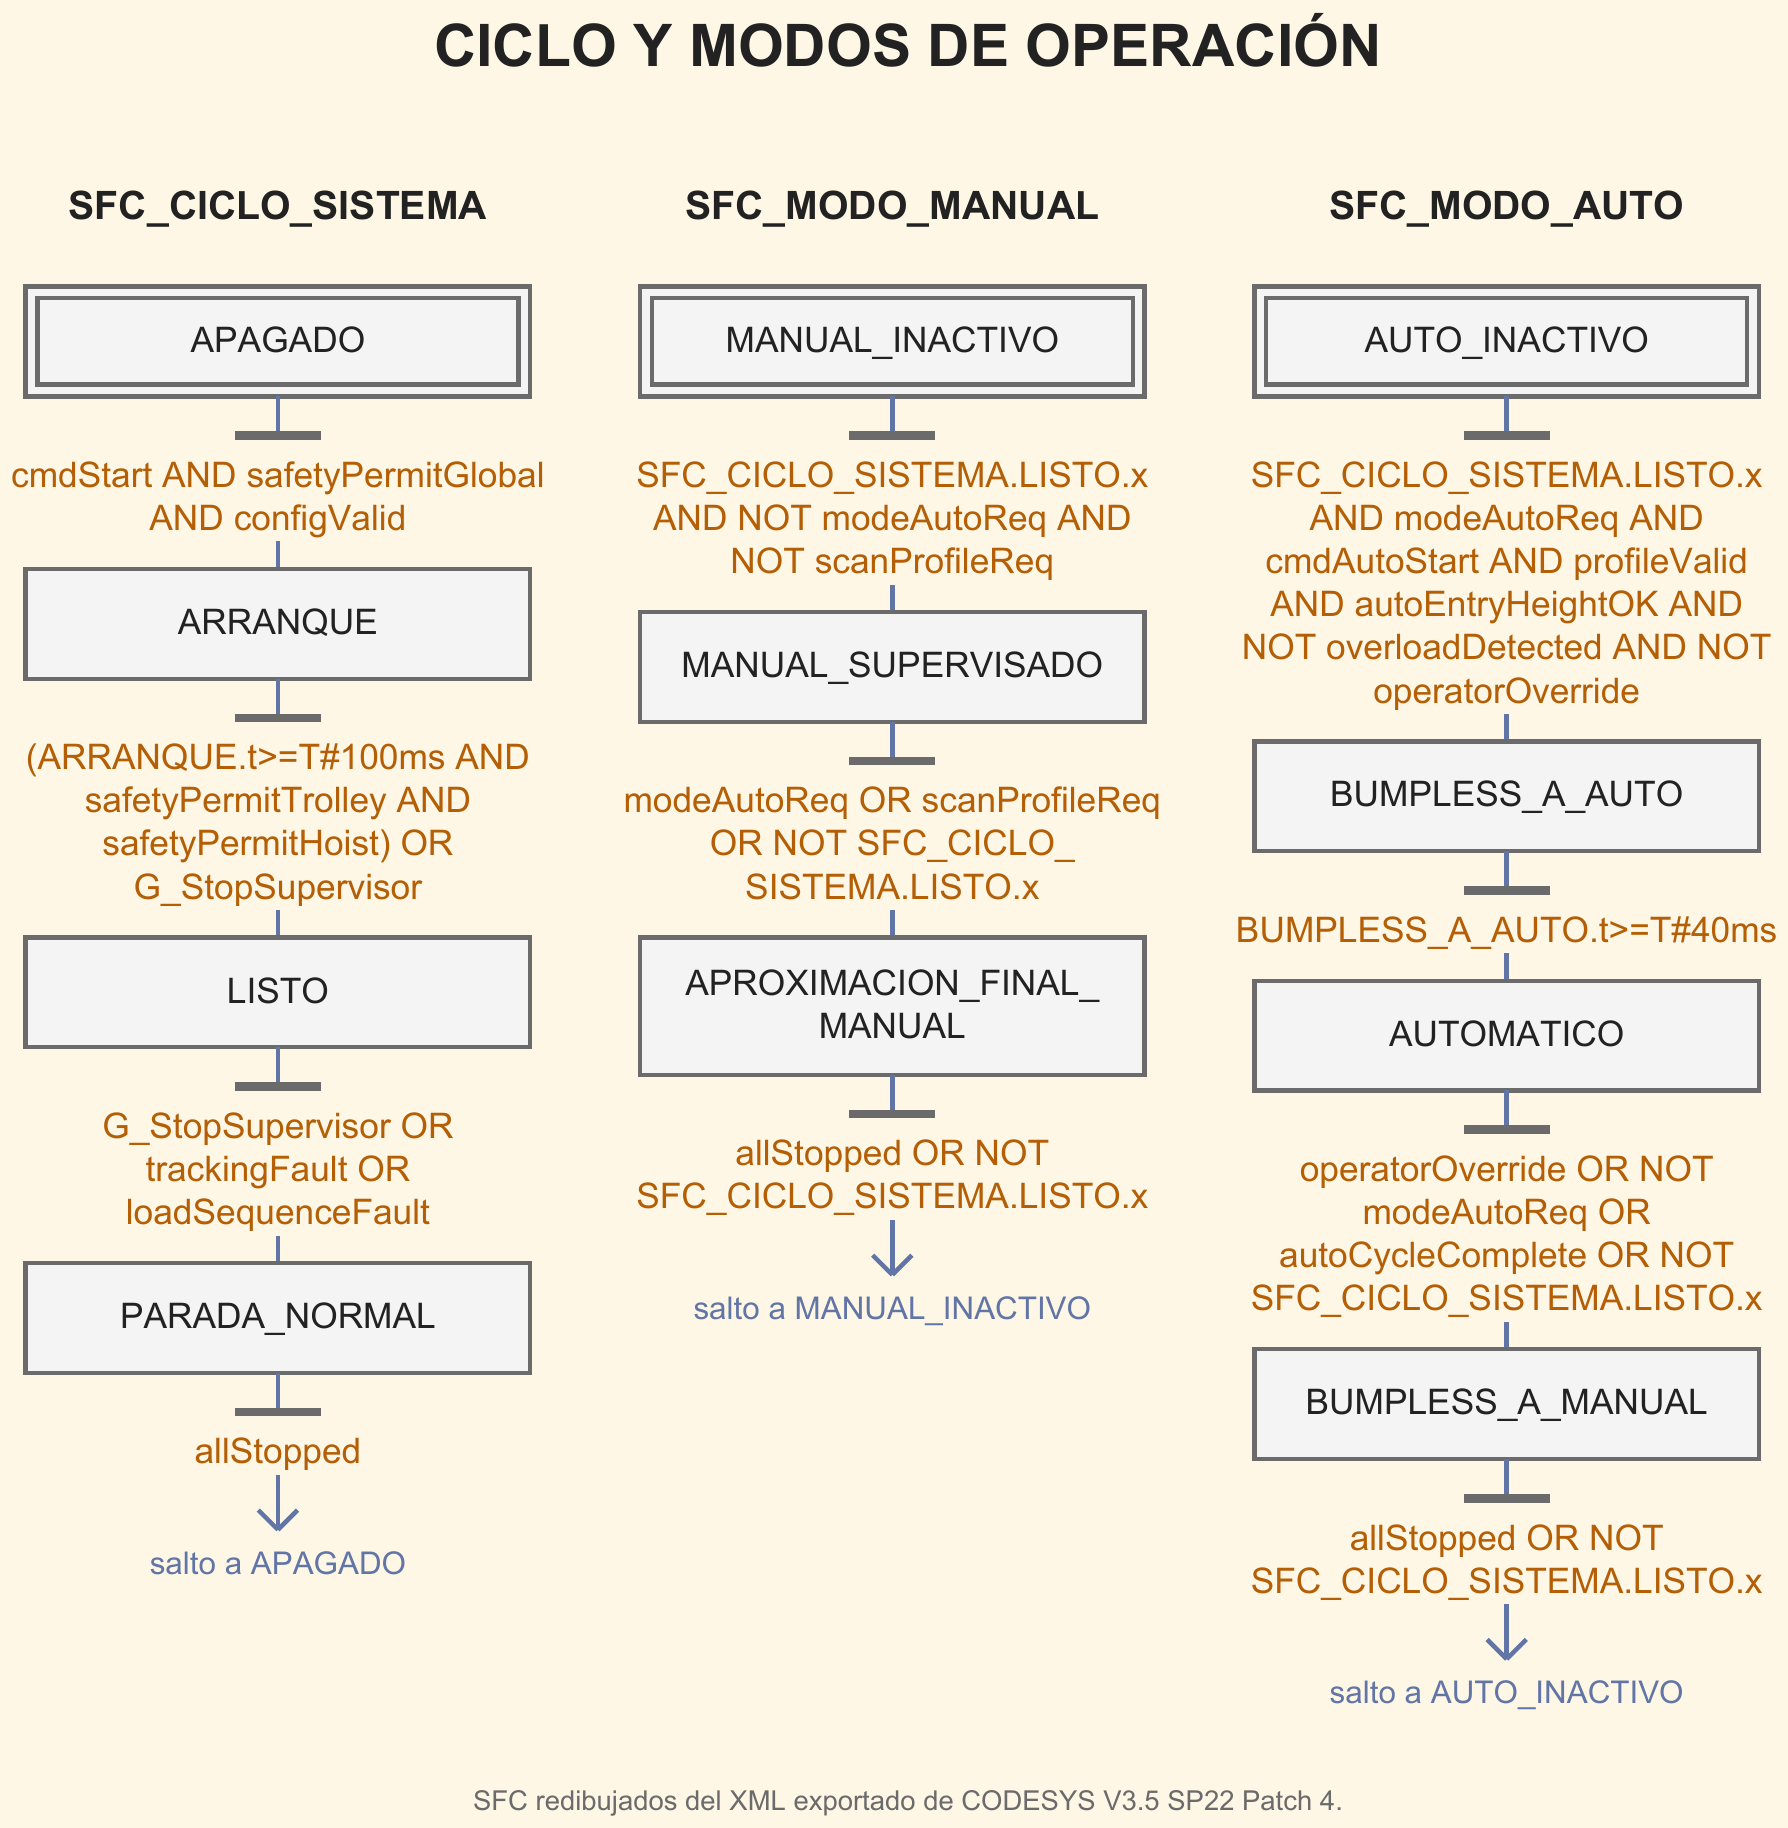
\includegraphics[width=15.0cm,height=6.35cm,keepaspectratio,trim=7.00bp 7.00bp 7.00bp 7.00bp,clip]{imagenes/r_051.png}}\par\note{Contrastar con Stateflow sin afirmar equivalencia formal de todas las transiciones.}
\end{frame}
\begin{frame}[t,label=slide99]{Respaldo: bajada de 8 m}
\relax
\figurefooter{Ensayo aislado con carga y spreader vacío.}
\vspace{-2mm}\makebox[\linewidth][c]{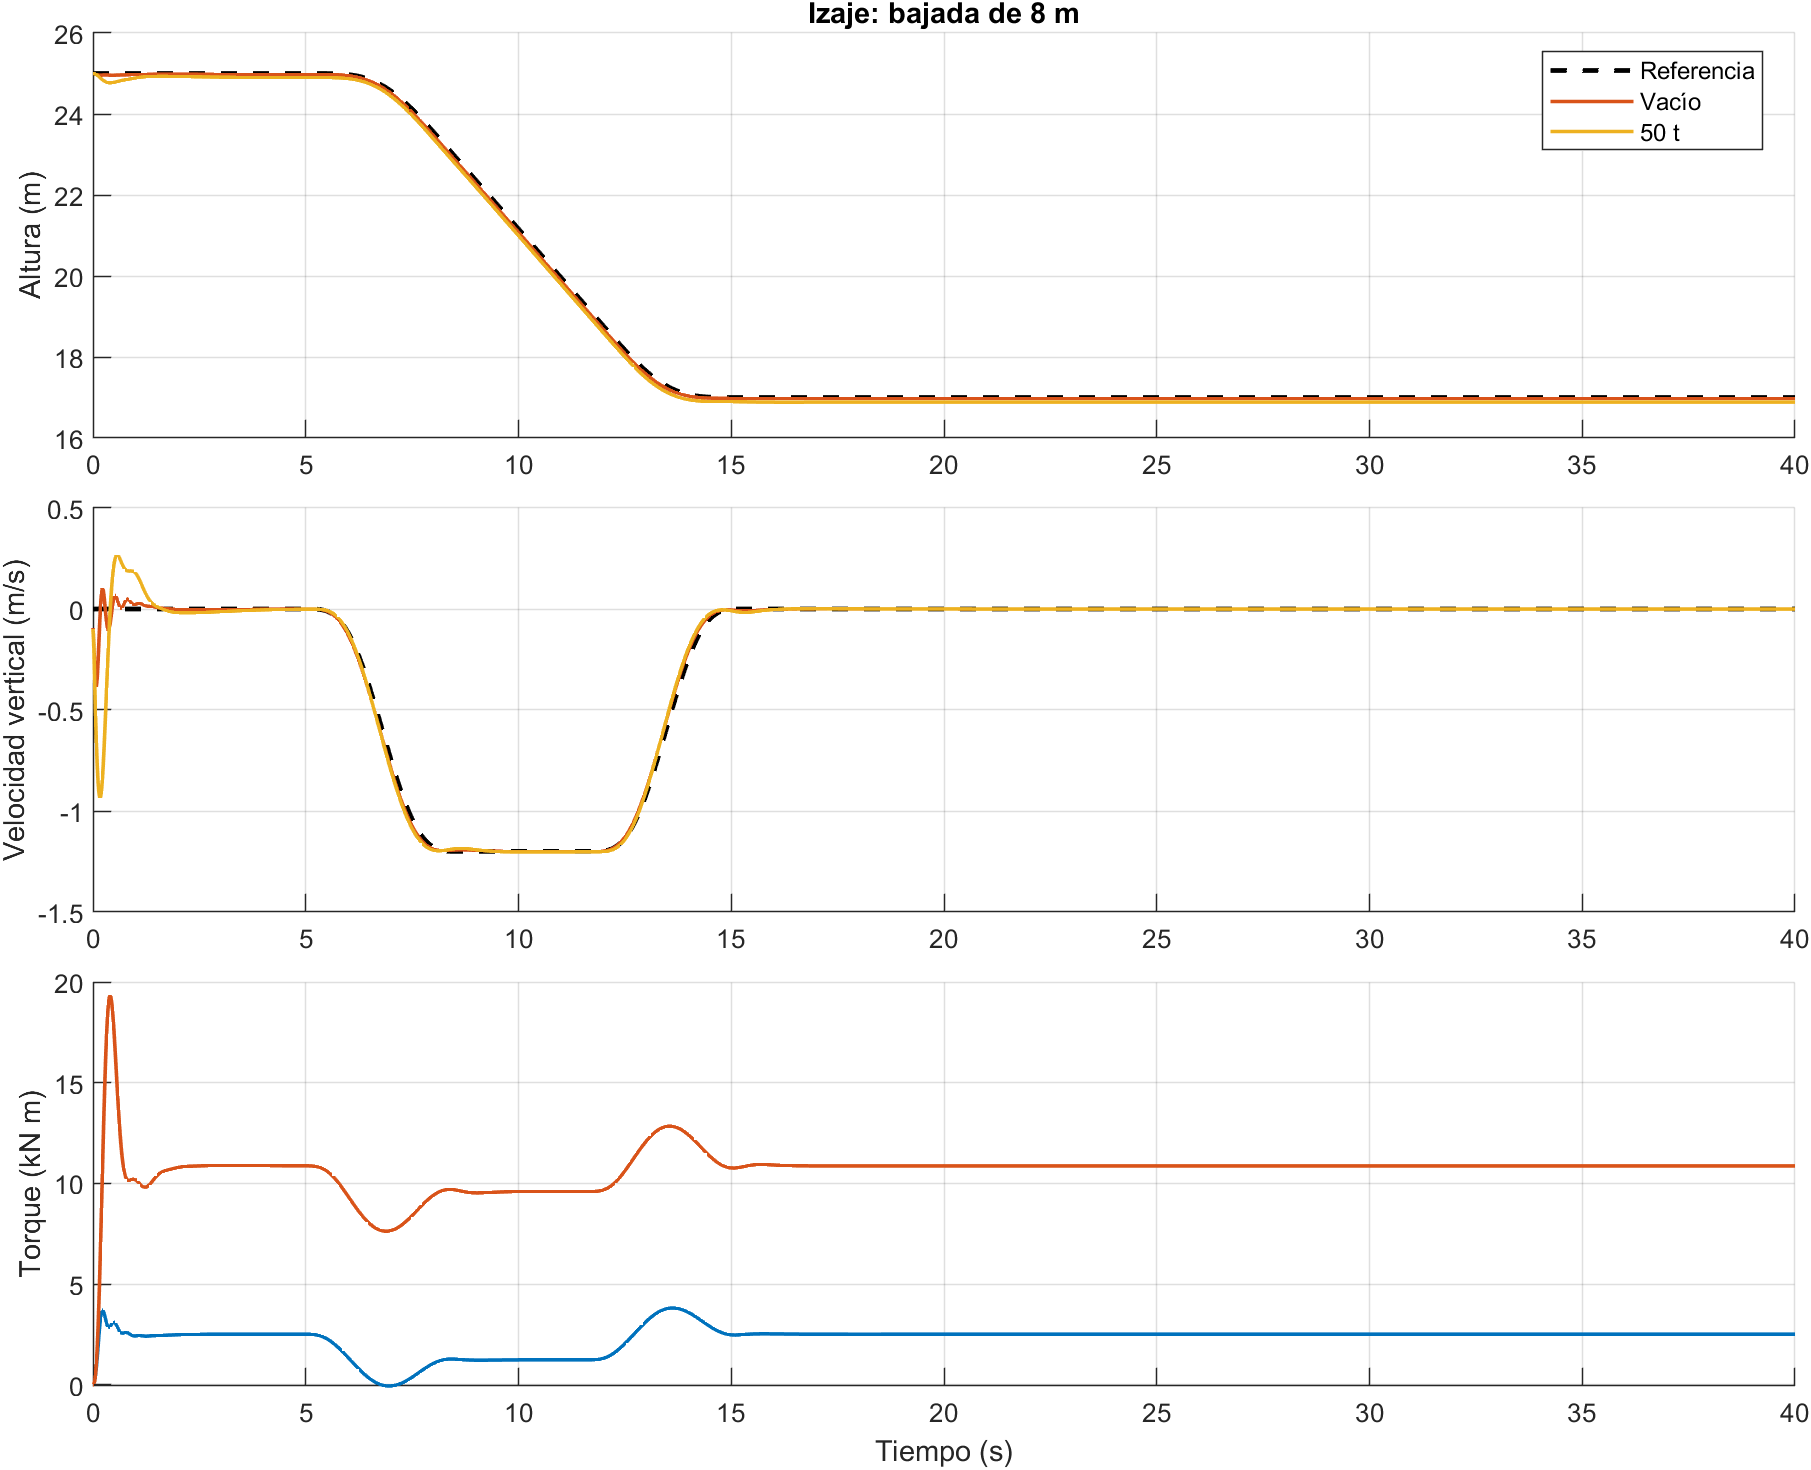
\includegraphics[width=15.0cm,height=6.35cm,keepaspectratio,trim=0.00bp 0.00bp 0.00bp 0.00bp,clip]{imagenes/r_040.png}}\par\note{Complementar los resultados de seguimiento vertical.}
\end{frame}
\begin{frame}[t,label=slide101]{Respaldo: torques de la prueba completa MIL}
\relax
\figurefooter{Consigna antes y después del limitador, y torque físico aplicado.}
\vspace{-2mm}\makebox[\linewidth][c]{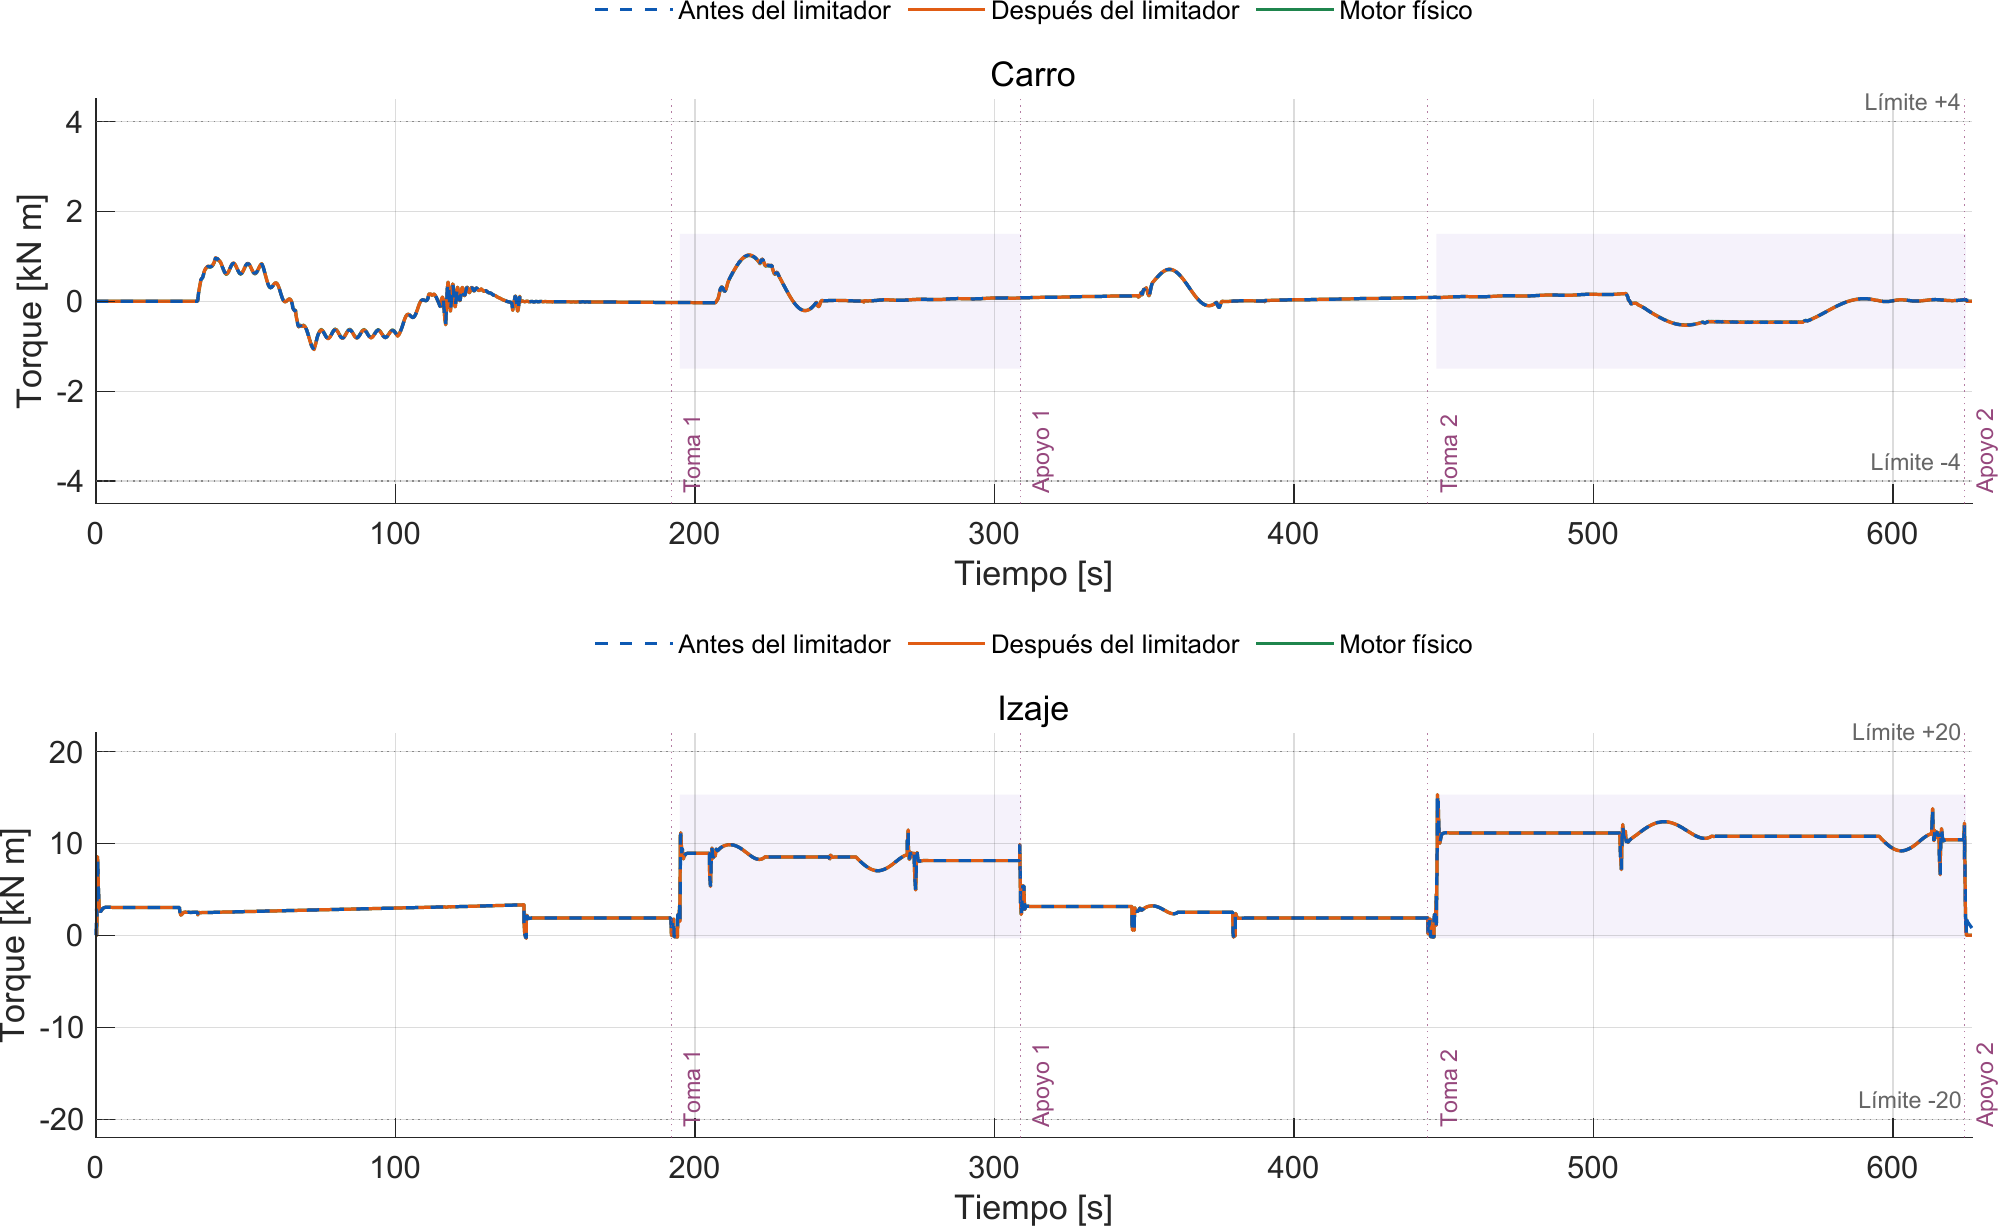
\includegraphics[width=15.0cm,height=6.35cm,keepaspectratio,trim=0.00bp 0.00bp 0.00bp 0.00bp,clip]{imagenes/r_071.png}}\par\note{Distinguir limitación de torque y respuesta dinámica del modulador.}
\end{frame}
\begin{frame}[t,label=slide102]{Respaldo: torques de la prueba completa SIL}
\relax
\figurefooter{Registros desde START; límites nominales de ambos ejes.}
\vspace{-2mm}\makebox[\linewidth][c]{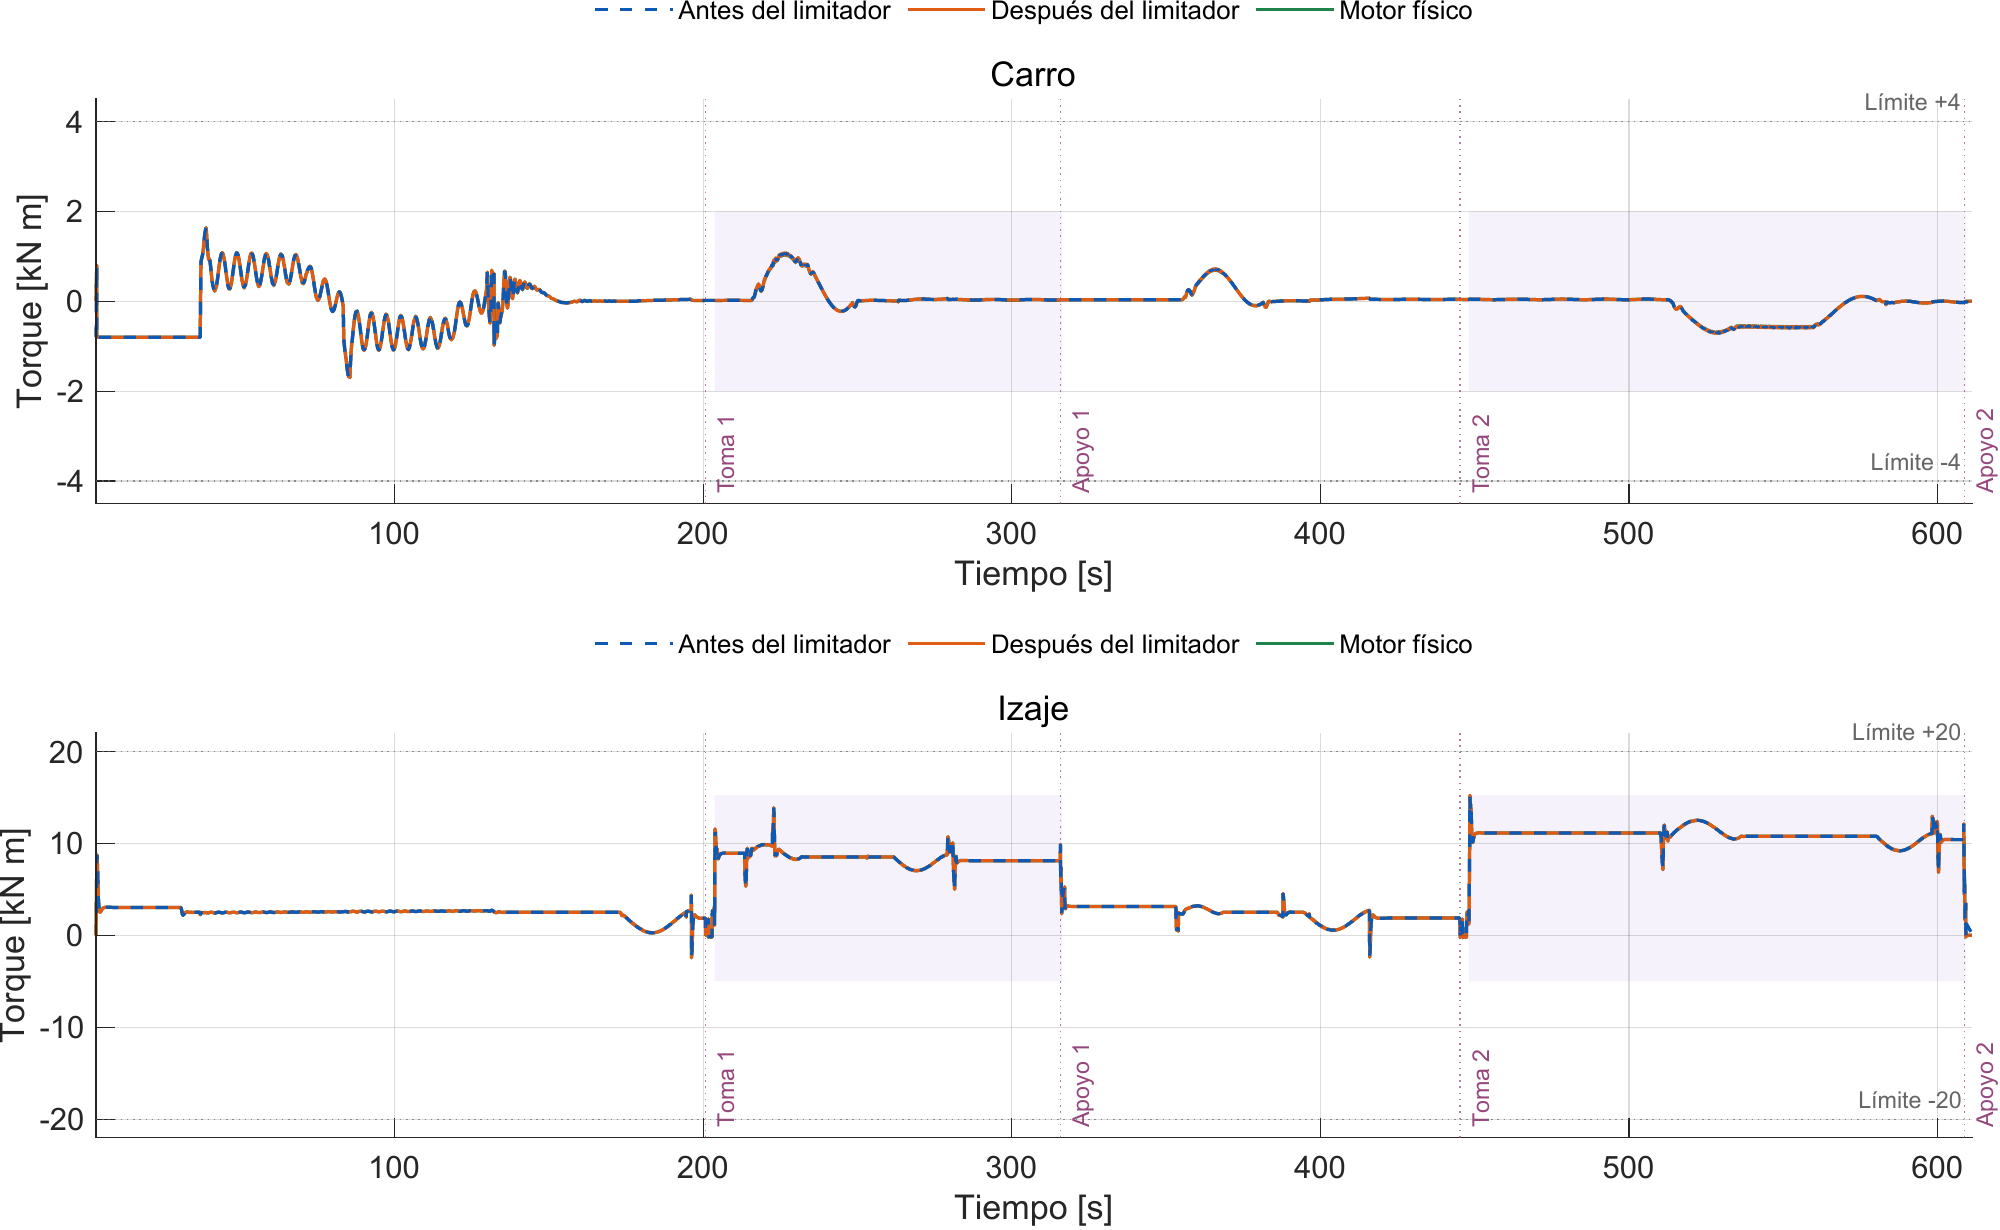
\includegraphics[width=15.0cm,height=6.35cm,keepaspectratio,trim=0.00bp 0.00bp 0.00bp 0.00bp,clip]{imagenes/r_080.png}}\par\note{Máximos1,699y15,212kNm. El torque físico no sirve por sísolo para identificar recorte.}
\end{frame}
\begin{frame}[t,label=slide103]{Respaldo: sin anti-sway, llegada sin entrega}
\relax
\figurefooter{Con y sin corrección: posiciones y referencias originales.}
\vspace{-2mm}\makebox[\linewidth][c]{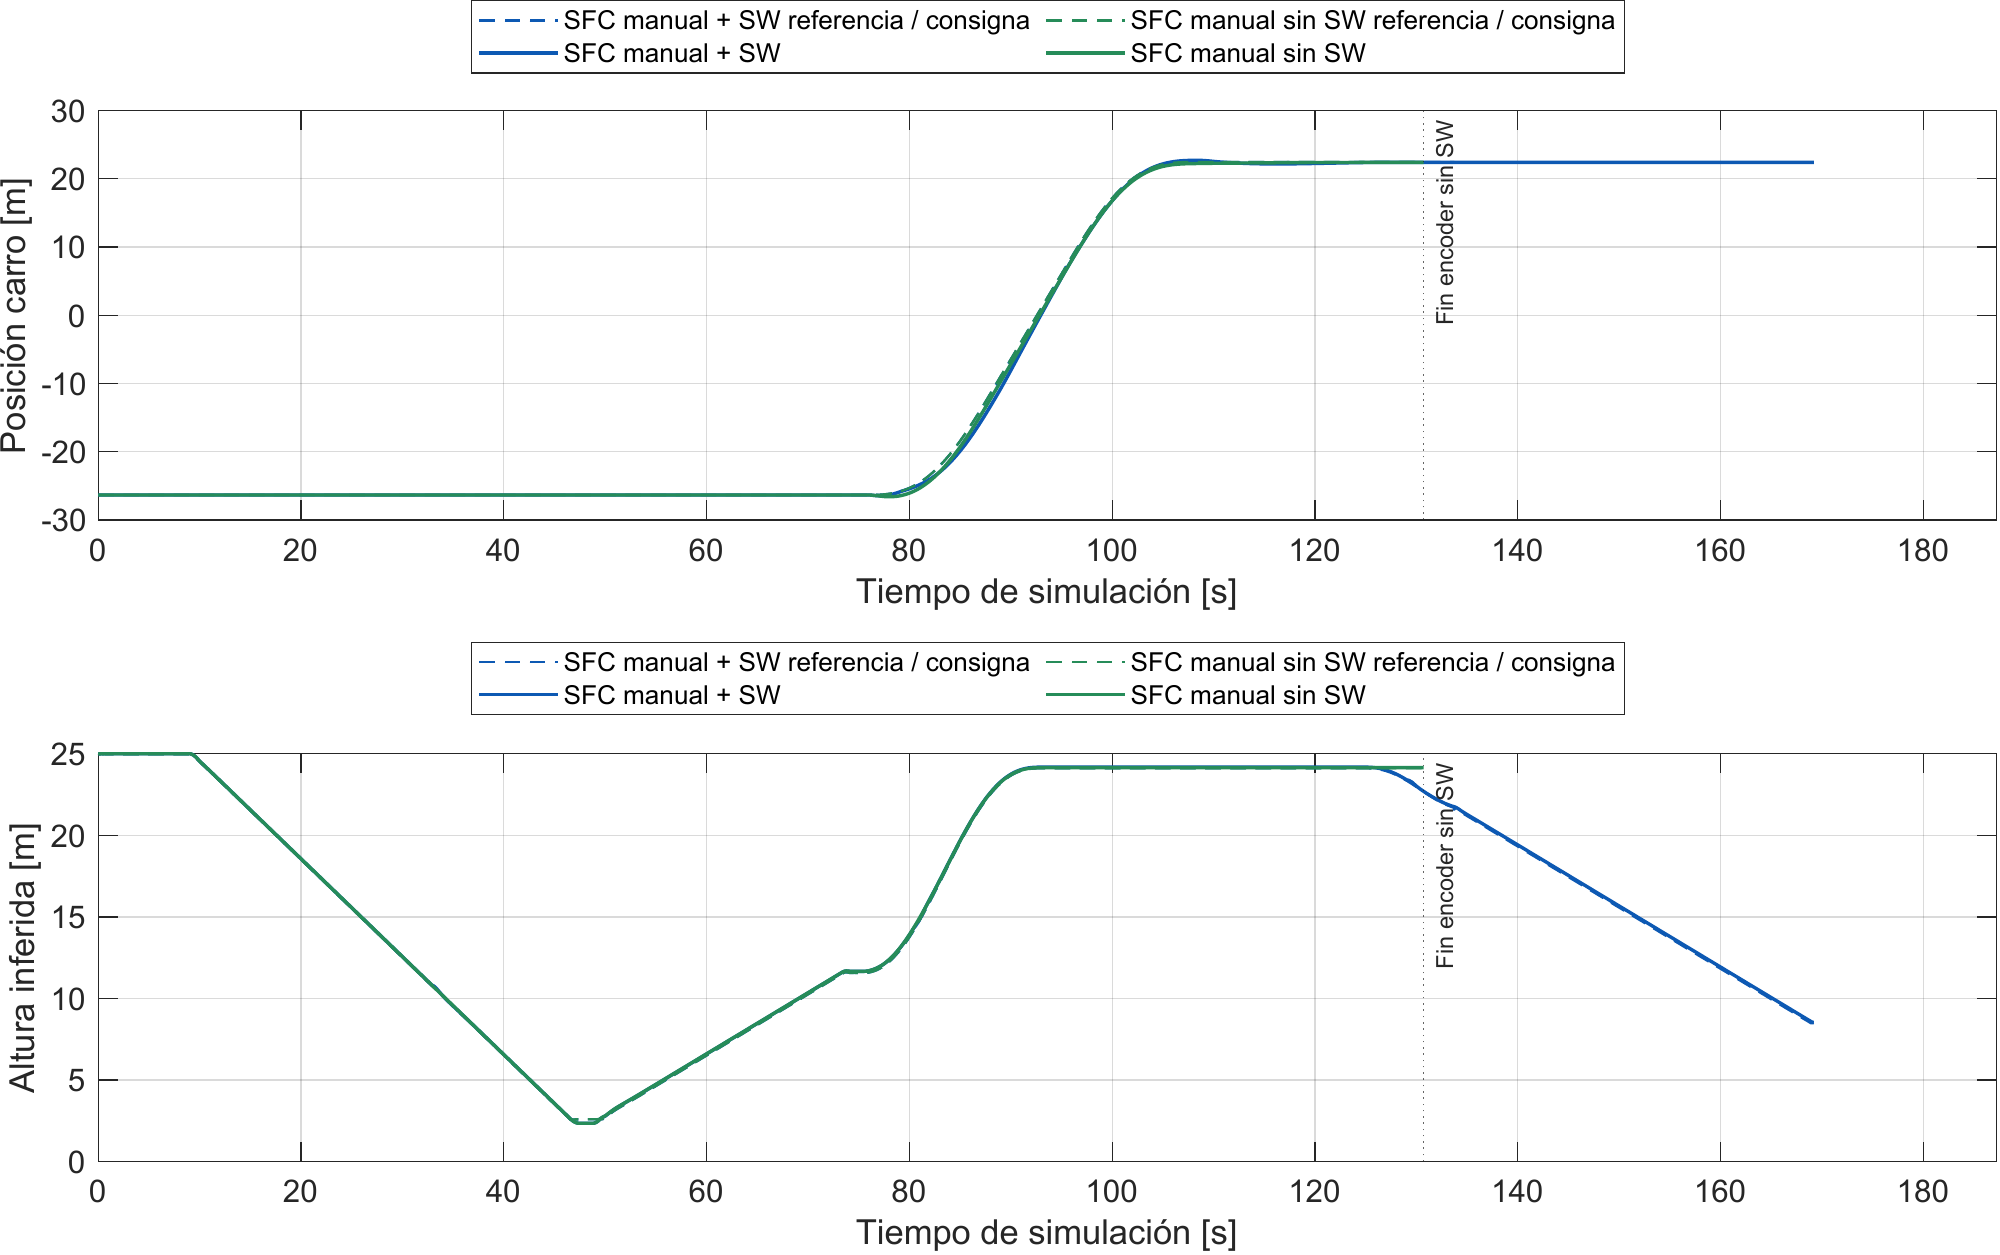
\includegraphics[width=15.0cm,height=6.35cm,keepaspectratio,trim=0.00bp 0.00bp 0.00bp 0.00bp,clip]{imagenes/r_093.png}}\par\note{Mostrar que el carro llega al destino pero la secuencia no continúa hacia la entrega.}
\end{frame}
\begin{frame}[t,label=slide104]{Respaldo: métricas y escalas de aceleración}
\begin{center}
{\small\renewcommand{\arraystretch}{1.0}
\begin{tabular}{p{5.1cm}p{8.4cm}}\toprule
Magnitud & Interpretación\\\midrule
Aceleración de referencia & Solicitada por el generador\\
Mando de aceleración & Suma del PI y anticipación, limitada\\
Aceleración de accionamiento & Reconstruida desde encoder / observador\\
Aceleración física del carro & Respuesta de la transmisión flexible\\
Aceleración física de carga & Incluye contactos y cable elástico\\
\bottomrule\end{tabular}}\end{center}
Las escalas de algunas gráficas del informe recortan transitorios; consultar los máximos documentados.
\note{MIL: pico vertical físico149,77m/s²encontacto. CODESYS:144,628m/s²físico; aceleración reconstruida5,938m/s²fuera del rango ±1 de la figura. Estos fenómenos son diferentes.}
\end{frame}
\begin{frame}[t,label=slide105]{Respaldo: configuración y fuentes de evidencia}
\begin{itemize}
\item Documentación final: ecuaciones, implementación y pruebas.
\item Documentación de pruebas completas MIL y SIL.
\item Pruebas de medio ciclo CODESYS del 08/10: comparación SFC/ST y sin anti-sway.
\item \texttt{PROD\_FINAL}: ciclos \texttt{MC\_prod\_DESAP} y \texttt{MC\_prod\_APROB} del 10/10.
\item Videos HMI acelerados 5×; se conservan sus metadatos.
\end{itemize}\vspace{4mm}\footnotesize Las imágenes de esta presentación se trazan en \texttt{fuentes\_figuras.json}.
\note{No agregar resultados de las corridas incompletas de prueba completa con el ajuste productivo. }
\end{frame}
\end{document}
